\documentclass[a4paper,debug,notitlepage,nobib]{tufte-book}

%%%%%%%%%%%%%
%Compilation options
%%%%%%%%%%%%%
%\newif\ifNotMonojetTTBarOnly

\usepackage[autokw=all]{svn-multi}[2015/05/12]
\svnidlong
{$HeadURL$}
{$LastChangedDate$}
{$LastChangedRevision$}
{$LastChangedBy$}
\svnid{$Id$}
\usepackage{graphicx}
\usepackage[svgnames]{xcolor}
\usepackage{hyperref}
\usepackage{lineno}
\usepackage{epstopdf}
% \usepackage{appendix}
\usepackage{xspace} %for single top
\usepackage{longtable} %for ttbar 
\usepackage{slashed}
\usepackage{amsfonts}
\usepackage{amsmath,amssymb}
\usepackage{slashed}
\usepackage{feynmp}
% begin feynman diagram setup
\usepackage{feynmp-auto}
% before setting default graphics include widths, save the default to properly scale feynman diagrams with their labels
\makeatletter
\let\ginnatwidth\Gin@nat@width
\let\ginnatheight\Gin@nat@height
\makeatother
\setkeys{Gin}{width=\linewidth,totalheight=\textheight,keepaspectratio}
%if you don't use the feynmandiagram environment for feynmf/mp figures, and you've changed the Gin keys above, then you need to manually adjust the unit length for feynman diagrams to get ratio of tex labels to graphics right. \unitlength = 1.21mm for tufte \linewidth and \textheight
\DeclareGraphicsRule{*}{mps}{*}{}
\newenvironment{feynmandiagram}[1][]{\setkeys{Gin}{width=\ginnatwidth,totalheight=\ginnatheight}\begin{fmffile}{#1}
\begin{fmfgraph*}(100,70)\fmfpen{thick}}{\end{fmfgraph*}\end{fmffile}\setkeys{Gin}{width=\linewidth,totalheight=\textheight,keepaspectratio}}
% end feynman diagram setup
\usepackage{subfig}
\DeclareGraphicsRule{*}{mps}{*}{}

\setkeys{Gin}{width=\linewidth,totalheight=\textheight,keepaspectratio}
\usepackage{mathtools} % extended mathematics
\usepackage{booktabs} % book-quality tables
\usepackage{units}    % non-stacked fractions and better unit spacing
\usepackage{multicol} % multiple column layout facilities
\usepackage{fancyvrb} % extended verbatim environments
\usepackage{fancyhdr}
\usepackage{refcount}
\usepackage{calc}
\usepackage{lastpage}
\usepackage{natbib} % for \citep
% create a dummy file (shell command "touch moderntex") to turn on some features that don't work on lxplus
\IfFileExists{moderntex}{
  \usepackage[protrusion=true,expansion=true,tracking=true,kerning=true,spacing=true]{microtype}
}{}
\fvset{fontsize=\normalsize} % default font size for fancy-verbatim environments

% Prints an asterisk that takes up no horizontal space.
% Useful in tabular environments.
\newcommand{\hangstar}{\makebox[0pt][l]{*}}
\newcommand{\openepigraph}[2]{%
  %\sffamily\fontsize{14}{16}\selectfont
  \begin{fullwidth}
  \sffamily\large
  \begin{doublespace}
  \noindent\allcaps{#1}\\% epigraph
  \noindent\allcaps{#2}% author
  \end{doublespace}
  \end{fullwidth}
}
\newcommand{\blankpage}{\newpage\hbox{}\thispagestyle{empty}\newpage}
\newcommand{\svnfooter}{Last Changed Rev: \svnfilerev}
\makeatletter
\title{ATLAS+CMS Dark Matter Forum Recommendations} 
\author{ATLAS+CMS Dark Matter Forum}
\date{\today}
\usepackage{titling}

%FIXME: interaction with front/backmatter?
%This is to make tufte append an Appendix in front of an appendix title, 
%even though Tufte himself might not have liked appendices?
%Taken from: https://groups.google.com/forum/#!topic/tufte-latex/oEWGA6624-Y
% \makeatletter% since we're using commands with @ in their name
\let\origappendix\appendix% save a copy of the original meaning of \appendix
\renewcommand{\appendix}{%
  \origappendix% do all the original \appendix stuff
  \titlecontents{chapter}%
    [0em] % distance from left margin
    {\vspace{1.5\baselineskip}\begin{fullwidth}\LARGE\rmfamily\itshape} % above (global formatting of entry)
    {\hspace*{0em}\appendixname~\thecontentslabel: } % before w/label (label = ``2'')
    {\hspace*{0em}} % before w/o label
    {\rmfamily\upshape\qquad\thecontentspage} % filler + page (leaders and page num)
    [\end{fullwidth}] % after
  \titleformat{\chapter}%
    [display]% shape
    {\relax\ifthenelse{\NOT\boolean{@tufte@symmetric}}{\begin{fullwidth}}{}}% format applied to label+text
    {\itshape\huge Appendix~\thechapter}% label
    {0pt}% horizontal separation between label and title body
    {\huge\rmfamily\itshape}% before the title body
    [\ifthenelse{\NOT\boolean{@tufte@symmetric}}{\end{fullwidth}}{}]% after the title body
  \setcounter{tocdepth}{1}
  \setcounter{secnumdepth}{1}
  %
  % Add any other special appendix-related code here.
  %
}
\makeatother% restore the special meaning of @
%restore the title


\linenumbers


%%%%%%%%%%%%%%%%%%%
%%%%%%%%%%%%%%%%%%%
%%%%%%%%%%%%%%%%%%%
%Symbols for Monojet section
\newcommand{\bra}[1]{\langle #1|}
\newcommand{\ket}[1]{|#1\rangle}
\newcommand{\MET}{\slashed{E}_T}
\newcommand{\mMed}{M_{\rm{med}}}
\newcommand{\gDM}{\ensuremath{g_{\rm{DM}}}\xspace}
\newcommand{\gq}{\ensuremath{g_{\rm q}}\xspace}
\newcommand{\ifb}{\rm{fb}^{-1}}
\newcommand{\mdm}{\ensuremath{m_{\rm{DM}}}\xspace}
\newcommand{\mmed}{\ensuremath{m_{\rm{med}}}\xspace}
\newcommand{\gdm}{\ensuremath{g_{\rm{DM}}}\xspace}
%%%%%%%%%%%%%%%%%%%
%%%%%%%%%%%%%%%%%%%
%%%%%%%%%%%%%%%%%%%
%Symbols for TTBar section
\def\invfb   {\ensuremath{\mbox{\,fb}^{-1}}\xspace}
\newcommand{\mev}{\ensuremath{\mathrm{\,Me\kern -0.1em V}}\xspace}
\newcommand{\mevc}{\ensuremath{{\mathrm{\,Me\kern -0.1em V\!/}c}}\xspace}
\newcommand{\mevcc}{\ensuremath{{\mathrm{\,Me\kern -0.1em V\!/}c^2}}\xspace}
\newcommand{\gev}{\ensuremath{\mathrm{\,Ge\kern -0.1em V}}\xspace}
\newcommand{\gevc}{\ensuremath{{\mathrm{\,Ge\kern -0.1em V\!/}c}}\xspace}
\newcommand{\gevcnospace}{\ensuremath{{\mathrm{\,Ge\kern -0.1em V\!/}c}}}
\newcommand{\gevcc}{\ensuremath{{\mathrm{\,Ge\kern -0.1em V\!/}c^2}}\xspace}
\newcommand{\bea}{\begin{eqnarray}}
\newcommand{\eea}{\end{eqnarray}}

\def\beq{\begin{equation}}
\def\eeq{\end{equation}}
\def\bea{\begin{eqnarray}}
\def\eea{\end{eqnarray}}

\newcommand{\gsim}{ \mathop{}_{\textstyle \sim}^{\textstyle >} }
\newcommand{\lsim}{ \mathop{}_{\textstyle \sim}^{\textstyle <} }
\newcommand{\ev}{{\rm eV}}
\newcommand{\kms}{{\rm km/s}}
\newcommand{\kev}{{\rm keV}}
\newcommand{\Mev}{{\rm MeV}}

\def\missET {\slashed{E}_T}
\def \bm#1{\mbox{\boldmath$#1$\unboldmath}} 
\def \myeq#1{(\ref{#1})}

%TODO: make sure all symbols are consistent...
%%%%%%%%%%%%%%%%%%%
%%%%%%%%%%%%%%%%%%%
%%%%%%%%%%%%%%%%%%%
%Symbols for monotop
\newcommand{\DMParticle}{\ensuremath{\chi}}
\newcommand{\be}{\begin{equation}}
\newcommand{\ee}{\end{equation}}
\newcommand\bpm{\begin{pmatrix}}
	\newcommand\epm{\end{pmatrix}}
\def\bsp#1\esp{\begin{split}#1\end{split}}
\renewcommand{\d}{{\rm d}} 
\newcommand{\etc}{{\it etc.}}
\newcommand{\ie}{{\it i.e.}}
\newcommand{\eg}{{\it e.g.}}
\newcommand{\lag}{{\cal L}} 
\newcommand{\gmu}{\gamma^\mu}
\newcommand{\feynrules}{{\sc FeynRules}}
\newcommand{\madgraph}{{\sc MadGraph}}
\newcommand{\madevent}{{\sc MadEvent}}
\newcommand{\madanalysis}{{\sc MadAnalysis}}
\newcommand{\fewz}{{\sc Fewz}}
\newcommand{\hathor}{{\sc Hathor}}
\newcommand{\pythia}{{\sc Pythia}}
\newcommand{\tauola}{{\sc Tauola}}
\newcommand{\delphes}{{\sc Delphes}}
\newcommand{\fastjet}{{\sc FastJet}}
\newcommand{\SUtwoUone}{\ensuremath{\mathrm{SU}(2)_{L} \times \mathrm{U}(1)_{Y}}\xspace}
\newcommand{\SUtwo}{\ensuremath{\mathrm{SU}(2)_{L}}\xspace}
\newcommand{\Lagr}{\ensuremath{\mathcal{L}}\xspace}
\newcommand{\fmet}{\ensuremath{f_{\mathrm{met}}}\xspace}
\newcommand{\met}{MET\xspace}
\newcommand{\ares}{\ensuremath{a_{\mathrm{res}}}\xspace}
\newcommand{\anonres}{\ensuremath{a_{\mathrm{non-res}}}\xspace}
\newcommand{\Xnew}{\ensuremath{X_{\mathrm{new}}}\xspace}
\newcommand{\BR}[2]{\ensuremath{\mathrm{BR}({#1} \to {#2})}\xspace}
\newcommand{\ssll}{\ensuremath{\ell^{+}\ell^{+}}\xspace}
\newcommand{\ttbarV}{\ensuremath{\ttbar V}\xspace}
\def\mfmet{\ensuremath{m(f_{\mathrm{met}})}}
\def\mvmet{\ensuremath{m(v_{\mathrm{met}})}}
\def\vmet{\ensuremath{v_{\mathrm{met}}}}
\def\fmet{\ensuremath{f_{\mathrm{met}}}}


\begin{document}

\morefloats
\setcounter{secnumdepth}{3} % turn on section numbering, for now (3=subsubsection)

% the title page and front matter

\thispagestyle{empty}% suppress header for this page
% title
%\frontmatter
{\noindent Version 0.1 DRAFT}
\topskip0pt
\vspace*{\fill}
\begin{fullwidth}
\sffamily
{
  \huge
  \smallcaps
  \@title
}\\
\vspace{4\baselineskip}
{\Large 
\noindent
\input contributors.tex
}\\
\vspace{4\baselineskip}
\noindent
\@date\\
\vspace{\baselineskip}
\end{fullwidth}
\vspace*{\fill}


\pagebreak

%\ifNotMonojetTTBarOnly
\chapter{Introduction}
\label{sec:Introduction}
\svnidlong
{$HeadURL$}
{$LastChangedDate$}
{$LastChangedRevision$}
{$LastChangedBy$}
\svnid{$Id$}

Many theories of physics beyond the Standard Model predict the existence
of a stable, neutral, weakly-interacting and massive particle that is
a putative dark matter candidate.   In the following, we refer to such
matter as dark matter, even though the observation of such matter at a collider
could only establish that it is neutral, weakly-interactive, massive and stable
on the distance-scales of 10's of meters.
Dark matter has not yet been observed in particle physics experiments, and
there is not yet any evidence for non-gravitational interactions
between dark matter and Standard Model particles.  If such
interactions exist, dark matter particles could be produced
at the LHC. Since dark matter particles of themselves do not produce signals
in the LHC
detectors, one way to observe them is when they are produced in association
with a visible SM particle X(=$g, q, \gamma, Z, W$, or $h$).
%% so simple pair-production of dark matter particles, for example,
%% would
%% not be visible.
%% However, there are different mechanisms by which a
%% could be produced in association with dark matter.
Such reactions, which are
observed as particles or jets recoiling against an invisible state, are
called ``mono-X'' or \MET{}+X reactions.
This type of reaction includes the production of a Higgs boson that
decays to pairs of dark matter particles.


Early Run-1 searches for \MET{}+X signatures at ATLAS and CMS employed
a basis of operators in 
effective field theories (EFTs) \cite{Goodman:2010yf,Goodman:2010ku} to
calculate the possible signals.
\Todo{Check these references here}
These particular EFTs assume that production of dark matter takes place through
a contact interaction involving a quark-antiquark pair or two gluons and
two dark matter particles.  In this case,
the missing
energy distribution of the signal is determined
by the mass of the dark
matter particles and the Lorentz structure of the interaction. Only the
overall production rate is a free parameter to be constrained or measured.
Both experiments studied a variety
of EFTs with different spin structures. Provided that the contact
interaction approximation holds, these EFTs can also provide a
straightforward way to compare the results from different collider
searches with non-collider searches for dark matter.  


The interpretation of some Run-1 LHC data as limits on contact interactions
provided results that were outside the range of applicability of the EFT
description, requiring some thought on how to handle this situation \cite{Bai:2010hh,Kopp:2011eu,Fox:2011fx,Fox:2011pm,Shoemaker:2011vi,Busoni:2013lha}.
Some ``simplified models'' \cite{Alwall:2008ag,Goodman:2011jq,Alves:2011wf}
of dark matter production
were constructed with particles and interactions beyond the SM ones.
These models can be used consistently at LHC energies,
and make some different predictions than the EFTs.
Many proposals for such models have emerged (see, for example
Refs. \cite{An:2012va,An:2012ue,Tait:2013,Buchmueller:2013dya,Bai:2013iqa,Bai:2014osa,An:2013xka,Yavin:14092893,Malik:2014ggr,Harris:2014hga,Buckley:2014fba,Haisch:2015ioa}). 
All of them introduce a new particle -- a mediator -- that allows
interactions between SM and DM particles.
In the limit of large mediator mass, these simplified models map onto
EFT operators.
%% that a contact
%% interaction is often not the correct description for the signals to
%% which the LHC is sensitive.
%Limits from the LHC on particles that are
%QCD singlets and do not decay to hard leptons are relatively
%weak (see, for example, limits on dijet resonances for weakly-coupled
%theories).
%Such particles can mediate reactions that produce dark matter
%particles.
If the mass of the mediator is light, the kinematics of the
dark matter production can differ substantially from that due to a contact
interaction, modifying limits and possibly requiring new search strategies.
Appropriate simplified models can be used both to
interpret mono-X searches and to guide the design of complementary
searches for additional signatures.

At the end of 2014, ATLAS and CMS organized a forum, the ATLAS-CMS Dark
Matter Forum, to form a consensus on the use of simplified models
and EFTs for Run-2 with the participation of experts on
theories of dark matter. This is the final report of that forum.

One of the guiding principles of this report is to channel the efforts
of the ATLAS and CMS Collaboration towards a minimal set of dark
matter models that should influence the design of the early Run-2
searches. At the same time, a thorough survey of realistic collider
signals of dark matter is a crucial input to the overall design of the
search program.

The goal of this report is such a survey, though confined within some
broad assumptions and focused on benchmarks for kinematically-distinct
signals which are most urgently needed. As far as time and resources
have allowed, the assumptions have been carefully motivated by
theoretical consensus and comparisons of simulations. But, to achieve a
true consensus in only a few months before the start of Run-2, it was
important to narrow the scope and timescale to the following:

\begin{enumerate}
\item The forum should propose a prioritized, compact set of benchmark
  simplified models that should be agreed upon by both collaborations for
  Run-2 searches. The values for the scan on the parameters of the models for which
  experimental results are provided should be specified, to facilitate theory reinterpretation 
  beyond the necessary model-independent limits that 
  should be provided by all LHC Dark Matter searches. 
\item The forum should standardize the event generator implementation
  of the simplified models and harmonize other common technical
  details as far as practical. It
  would be desirable to have a common choice of LO/NLO, ME-parton
  shower matching and merging, factorization and renormalization
  scales for each of the simplified models. This will also lead to a
  common set of theory uncertainties, which will facilitate the
  comparison of results between the two collaborations.
\item The forum could also discuss how to apply the
  EFT formalism and present the results of EFT
  interpretations.
\item The forum should prepare a report summarizing these items,
  suitable both as a reference for the internal ATLAS and CMS
  audiences and as an explanation for theory and non-collider
  readers. This report represents the views of the participants of the
  forum.
\end{enumerate}

\section{Grounding Assumptions}

We assume that interactions exist between Standard Model hadrons
and whatever constitutes cosmological dark matter. If this
is not the case, then proton collisions will not produce dark matter
particles, and dark matter will not scatter off nuclei in direct
detection experiments.

The Dark Matter itself is assumed to be a single particle, a Dirac
fermion WIMP, stable on collider timescales and non-interacting with
the detector.  
The former assumption is reductionistic.
The rich
particle content of the Standard Model is circumstantial evidence that
the dark matter sector, which constitutes five times as much of the
mass of the universe, may be more complex than a single particle or a
single interaction. But, as was often the case in the discoveries of
the SM, here only one mediator and one search channel might play a
dominant role in the opening stages of an LHC discovery. The latter
assumption focuses our work on early LHC searches, where small
kinematic differences between models will not matter in a discovery
scenario, and with the imminent re-start of the LHC our report relies
heavily on a large body of existing theoretical work which made this
assumption. Different types of dark matter particles will typically
give similar results.
Some exceptions exist:  the choice of Dirac fermions forbids some
processes that are allowed for Majorana fermions.
Aside from this, the cases
of Dirac or Majorana fermions or scalars produces only minor changes
in the kinematic distributions of the visible particle, especially
when considering cut-and-count\sidenote{Cut-and-count refers to an analysis
that applies a certain event selection and checks the inclusive number of events which pass.   This is to be constrasted with a shape analysis that compares the distribution of events.} analysis. Thus the choice of Dirac
fermion dark matter is deemed sufficient for the benchmarks aiding the
design of the upcoming Run-2 searches. Nevertheless, a more complete
set of models will certainly be required upon a discovery; see
e.g.~\cite{Cotta:2012nj,Haisch:2013fla,Crivellin:2015wva} for some
studies of observables that may distinguish amongst these models.

The weakness of the dark matter--visible matter interactions is explained
by assuming a mediating force or particle that indirectly connects the
two.  In the EFT approach, the mass scale of the mediator is assumed
to be large compared to the typical momentum involved in the production
of dark matter.   Since EFTs have been established for some time,
we focus on 
simplified models that allow the exploration of scenarios where the
mediating scale is not so large.
%because the EFT approach, viable for the
%other types of dark matter searches, breaks down at the LHC. Another
%way of viewing this problem is that any BSM model of dark matter
%requires at least two particles: a dark matter candidate and a
%mediator of the interaction between the dark matter and the Standard
%Model.
One strength of collider experiments lies in the ability to
study the mediator, not just the DM. A discovery of an
anomalous \MET signature
at the LHC would not uniquely imply discovery of dark matter, while at
the same time discovery of an anomalous and annually-modulated signal
in a direct-detection experiment would leave unanswered many questions
about the nature of the interaction. The these two approaches, and
other types of non-collider searches, provide complementary ways to
approach the problem, and it is in this spirit that our focus is on
the mediator. We systematically explore the basic possibilities for
mediators of various possible spins and couplings.
All models are assumed to produce a signature with pairs of dark matter particles.
Though more varied and
interesting possibilities are added to the literature almost daily,
these basic building blocks account for much of the physics studied at
hadron colliders in the past three decades.


We also assume that Minimal Flavor Violation (MFV) \cite{Chivukula:1987py,Hall:1990ac,Buras:2000dm,D'Ambrosio:2002ex} applies to the
recommended models. This means that the flavor structure of the
couplings between dark matter and ordinary particles follows the same
structure as the Standard Model. This choice is simple, since no
additional theory of flavor is required, beyond what is already
present in the SM, and it provides a mechanism to ensure that the
models do not violate flavor constraints.  As a consequence, spin-0
resonances must have couplings to fermions proportional to the SM Higgs couplings. Flavor-safe models can still be constructed beyond the MFV
assumption, for example ~\cite{Agrawal:2014aoa}, and deserve further study.
%cite Dolan:2014ska? Also DM@LHC report, if out in time. 

In the parameter scan for the recommended models, we make the
assumption of a minimal decay width for the particles mediating the
interaction between SM and DM.  This means that only decays
strictly necessary for the self-consistency of the model (e.g.  to DM
and to quarks) are accounted for in the definition of the mediator
width. We forbid any further decays to other invisible particles of
the Dark Sector that may increase the width or produce striking, visible signatures. Studies within the Forum
show that, for cut-and-count analyses, the kinematic distributions of
many models and therefore the sensitivity of the search do not depend
significantly on the mediator width, as long as the width remains smaller
than the mass of the particle.


The particle content of the models chosen as benchmarks is limited to
one single kind of DM whose self-interactions are not relevant for LHC
phenomenology, and to one type of SM/DM interaction at a time. These
assumptions only add a limited number of new particles to the
SM. These simplified models, independently explored by different
experimental analyses, can be used as starting points to build more
complete theories. Even though this factorized picture does not always
lead to full theories and leaves out details that are necessary for
the self-consistency of single models (e.g. the mass generation for
mediator particles), it is a starting point to prepare a set of
distinct but complementary collider searches for Dark Matter, as
it leads to benchmarks that are easily comparable across channels.

Contact interaction operators (EFTs) are also part of this report, 
to be considered whenever neither a simplified model completion 
nor other simplified models 
yielding similar kinematic distributions are available. 
This is the case for dimension 5-7 operators with direct 
Dark Matter-electroweak boson couplings. 
Model-independent results should be emphasized 
in the signal regions that are unique to these models, 
and results should be considered with the necessary caution due to EFT 
validity issues covered in the last chapter in this report. 
Results from these models may nevertheless help validate the 
contact interaction limit of new simplified models developed to complete 
these specific operators. 

The first chapter of the report is dedicated to simplified
models with radiation of a hard object either from the initial state
or from the mediator. These models produce primarily monojet signatures, 
but are recommended for all \MET{}+X searches.
Details of the implementation of these models in
Monte Carlo generators are provided in
Appendix \ref{app:MonojetLikeModels_Appendix}.
%Chapter~\ref{subsec:DMHFModels} describes the specific details of the general models
%for final states including heavy flavor quarks, leaving the implementation
%details to appendix~\ref{app:TTBar_Xsecs}.  
Chapter~\ref{subsec:EWSpecificModels} contains the benchmark model
recommendations and choices for final states specifically containing an electroweak 
boson ($W/Z/\gamma/H$). In this case, both
simplified models leading to mono-boson signatures
and contact interaction operators wherever simplified models are not available are considered. 
The final chapter is devoted to the treatment of the validity of benchmark
models from contact interaction operators.
The technical implementation and further models that can be studied
beyond early searches are in appendix~\ref{app:EWSpecificModels_Appendix}. 
Appendix~\ref{app:Presentation_Of_Experimental_Results} contains the necessary elements that
should be included in the results of experimental searches to allow for further reinterpretation. 
%The Appendices also collect information about the implementation of the
%models in event generator tools, as well as tables of expected cross sections.
%%This could be saved for monotop
%Appendix~\ref{app:ExtraModels} contains a series of models that produce interesting \MET{}+X signatures. 
%These models are not specifically recommended by the Forum as they
% deviate from the general assumptions made in this introduction. 
%They have however been used in previous ATLAS and CMS analyses and discussed thoroughly within the Forum. 
%They are therefore worth considering for early Run-2 searches, since they lead to unique signatures 
%that are not produced by any other of the recommended models. 
%\fi



%\fi

%\ifNotMonojetTTBarOnly
\chapter{Overall choices for simplified models}
\label{sec:SimplifiedModelsIntro} 
\svnidlong
{$HeadURL$}
{$LastChangedDate$}
{$LastChangedRevision$}
{$LastChangedBy$}
\svnid{$Id$}

Dark matter has not yet been seen in particle physics experiments, and
there is no evidence for non-gravitational interactions between dark
matter and Standard Model particles.  If such interactions exist,
pairs of dark matter particles could be produced at the LHC, leading
to so-called 'mono--X' signatures.

Run 1 searches for 'mono--X' signatures at ATLAS and CMS employed an
effective field theory \cite{Goodman:2010ku} to quantify the reach of
the analyses and to allow comparison with direct dark matter detection
experiments. There were several reasons for this.  First, the
presentation is model independent.  Secondly, the approach is
economical, requiring only a few simulated datasets.  Finally, at the
time, there was no catalogue of alternative interpretations of the
data. The downside of the EFT approach is that many of the implicit
limitations were not widely understood.

From the Run 1 results, it has become clear \cite{Busoni:2013lha} that
a contact interaction is often not the correct description for such
signals. The LHC is exploring a regime where the mediating process may
play a more interesting role, leading to missing energy signals that
can be kinematically distinct from those predicted by the EFT, as well
as qualitatively different signatures requiring new search
strategies. While the EFT integrates out the degrees of freedom of the
(heavy) intermediate particle, concrete ``simplified models'' with
low-mass mediators \cite{Alves:2011wf} can describe this richer
phenomenology. Such models can be used both to interpret mono-­X
searches and to guide the design of complementary searches for
additional signatures. Many proposals for such models began to emerge;
see for example
Refs. \cite{Tait:2013,Buchmueller:2013dya,Yavin:14092893,Malik:2014ggr,Harris:2014hga,Buckley:2014fba}.

To form a consensus on the simplified models most appropriate to use,
at the end of 2014 ATLAS and CMS organized a forum, the ATLAS-­CMS
Dark Matter Forum, whereby all interested experimenters from both
collaborations would discuss a minimal common set of Run-2 dark matter
interpretations with the participation of experts on theories of dark
matter. This is the final report of that forum.

To achieve a true consenus with only a few months before Run 2 would
bein, it was important to narrow the scope and timescale of this
forum. These were the goals:

\begin{enumerate}
\item A prioritized, small set of benchmark simplified models should
  be agreed upon by both collaborations for Run-2 searches.
\item The matrix element implementation of the simplified models
  should be standardized, and other common technical details (order of
  the calculation, showering) harmonized as much as practical. It
  would be desirable to have a common choice of LO/NLO, ME-­parton
  shower matching and merging, factorization and renormalization
  scales for each of the simplified models. This will also lead to a
  single set of theory uncertainties, which will be easier to deal
  with when comparing results from the two collaborations.
\item The forum could also discuss the conditions under which the EFT
  interpretation may still be desirable.
\item The forum should prepare a report summarising these items,
  suitable both as a reference for the internal ATLAS and CMS
  audiences and as an explanation for theory and non-collider
  readers. This report represents the views of the participants of the
  forum.
\end{enumerate}

%CD: I don't like this paragraph. 

There has indeed arisen a consensus on a handful of simple models
of dark matter production that have a hope of mapping into a more
complete theory.  This document describes them.  Also, in some cases,
there is no good alternative to using EFT.  Even in the case of simplified
models, we recommend showing the EFT limit.

%%CD: I don't really like the following paragraphs either. I'll be pickier tomorrow. 

One of the guiding principles of this report is to channel the efforts
of the ATLAS and CMS Collaboration towards obtaining experimental
results, rather than on providing elaborate interpretations and
re-interpretations of these results. At the same time, a thorough
survey of realistic collider signals of dark matter is a crucial input
to the design of such searches.

The goal of this report is such a survey, though confined within some
broad assumptions and focused on benchmarks for kinematically-distinct
signals which are most urgently needed for the early Run-2 mono-X searches. As
far as time and resources have allowed, the assumptions have been
carefully motivated by theoretical consensus and comparisons of simulation.

The first choice made for the Run-2 benchmarks is on the nature of the
Dark Matter itself: it is assumed to be a particle, stable on collider
timescales and non-interacting with the detector, and a Dirac fermion.
The latter is a practical choice, given that the Forum relied upon a large body of theoretical work which made the same assumption. Many of the conclusions in this
report should also apply to MET signals of Majorana fermion DM or
scalar DM with some minor modification to account for their different
angular distributions, especially when considering cut-and-count
analysis. Thus the choice of Dirac fermion dark matter is deemed
sufficient for the benchmarks aiding the design of the upcoming Run-2
searches. Nevertheless, a more complete set of models will certainly
be required upon a discovery; see e.g.~\cite{Crivellin:2015wva} for an
example of an observable that may distinguish the spin of the DM
particle.

We also assume that Minimal Flavor Violation (MFV) applies 
to the recommended models. This means that 
the flavor structure of the couplings between dark matter and ordinary particles
follow the CKM matrix. This choice is both natural, as there is no required 
additional theory of flavor beyond what is already present in the SM, and 
and useful to find benchmarks that are not already ruled out by flavor constraints. 
As a consequence, spin-0 resonances exchanged in the s-channel 
must have Yukawa coupings to SM fermions. Flavor-safe models can still 
be constructed beyond the MFV assumption~\ref{Agrawal:2014aoa},
but their phenomenology is left for future studies. 
%cite Dolan:2014ska? Also DM@LHC report, if out in time. 

In the parameter scan for the recommended models, we make the assumption
of minimal width for the particles mediating the interaction between SM and DM. 
This means that only the decays that are strictly necessary for the self-consistency of the model (e.g.
to DM and to quarks) are accounted for in the definition of the mediator width. In turn,
this forbids any further decays to other invisible particles of the Dark Sector that may increase
the width option. However,  studies within the Forum show that, 
for cut and count analyses, the kinematic distributions of many models and therefore the sensitivity of the search
do not depend significantly on the mediator width up to extreme values.  

The particle content of the models chosen as benchmarks is limited to one single kind of DM
whose self-interactions are not relevant for LHC phenomenology, and to one type of 
SM/DM interaction at a time. These assumptions only add a limited number of new particles
to the SM. These simplified models, independently sought by different experimental analyses,
can be used as starting points to build more complete theories. Even though 
this factorized picture does not always lead to full theories and leaves out details that are necessary
for the self-consistency of single models (e.g. the mass generation for mediator particles), 
it is a starting point to prepare a set of distinct but yet complementary collider searches for Dark Matter, 
as it leads to benchmarks that are easily comparable across channels. 

%\fi

\chapter{Recommended models for all MET+X analyses}
\label{subsec:MonojetLikeModels}
\svnidlong
{$HeadURL$}
{$LastChangedDate$}
{$LastChangedRevision$}
{$LastChangedBy$}
\svnid{$Id$}


% preamble

In this Chapter we review 
models that yield $X$+\MET{} signatures,
where $X$ is a QCD parton or $\gamma, W, Z$ or $h$.

The primary simplified models  for Dirac fermion DM endorsed by this Forum are detailed in this Chapter, 
comprising \spinzero and \spinone mediators. Section~\ref{sec:monojet_V} covers the
\schannel exchange of a vector mediator~\footnote{Colored vector mediators 
can be exchanged in the \tchannel, but there are no examples in literature so far.}, 
while we consider both \schannel and \tchannel exchange for scalar mediators in
Section~\ref{sec:monojet_scalar} and~\ref{sec:monojet_t_channel} respectively. 
\Spintwo mediators are briefly mentioned in Section~\ref{sec:spintwo}.
While these models are general and cover a broad set of signatures,
the discussion and studies are focused on the monojet final state. 
Details on final states with EW boson radiation and with heavy flavor quarks 
from diagrams arising within these models are also discussed in this Chapter.
%In the following paragraphs we present the peculiarities of these models that arise in the case of
%boson radiation, and present some examples of the relevant distributions for these final states.

The simplified model where a vector mediator is exchanged in the \schannel 
is known to NLO accuracy in the case of DM pair production in association to one parton~\cite{Haisch:2013ata}. 
All other models are currently known to leading order. Appendix~\ref{app:MonojetLikeModels_Appendix}
details the recommended implementation of these models that
have been used for the studies in this Chapter. A summary of the recommendation of the generation of this model
is provided in Table~%\ref{tab:summaryModels} % hardwire, because we don't use real caption on that table.
6.1.

%%%%%%%%%%%%%%%
%%%%%%%%%%%%%%%
%%%%%%%%%%%%%%%
% V/A SIMPLIFIED MODELS%
%%%%%%%%%%%%%%%
%%%%%%%%%%%%%%%
%%%%%%%%%%%%%%%

\section{Vector and axial vector mediator, \schannel exchange}
\label{sec:monojet_V}

A simple extension of the Standard Model (SM) is an
additional $U(1)$ gauge symmetry, where a dark matter (DM)
candidate particle has charges only under this new group.
Assuming that some SM particles are also charged under
this group, a new gauge boson can mediate interactions
between the SM and DM.   

%Lagrangian
We consider the case of a DM particle \chiDM of mass \mdm that is a Dirac fermion and where the production 
proceeds via the exchange of a \spinone mediator of mass \mMed in
the \schannel, illustrated in Fig.~\ref{fig:OP}.

\begin{figure}[h!]
\centering
  \unitlength=0.005\textwidth
  \vspace{0.5\baselineskip}
  \begin{feynmandiagram}[modelVmonojetParameters]
    \fmfleft{i1,i2}
    \fmfright{o1,o2}
    \fmftop{isr}
    \fmfbottom{pisr}
    % \fmf{dashes,tension=0.6,label={$\substack{{\Large V,,A}\\(m_{med},,\Gamma_{min,,med})}$}}{v1,v2}
    \fmf{wiggly,tension=0.6,label={\Large $V,,A(\mMed)$}}{v1,v2}
    \fmf{fermion}{o2,v2,o1}
    \fmf{fermion}{i2,visr,v1}
    \fmf{plain}{v1,pvisr,i1}
    \fmf{fermion,tension=0}{v1,i1}
    \fmfdot{v1,v2}
    \fmflabel{\Large ${g_q}$}{v1}
    \fmflabel{\Large ${g_{DM}}$}{v2}
    \fmflabel{\Large ${\bar{q}}$}{i1}
    \fmflabel{\Large ${q}$}{i2}
    \fmflabel{\Large ${\bar{\chiDM}(\mDM)}$}{o1}
    \fmflabel{\Large ${\chiDM(\mDM)}$}{o2}
    \fmf{gluon,tension=0}{visr,isr}
    \fmf{phantom,tension=0}{pvisr,pisr}
    \fmflabel{\Large ${g}$}{isr}
  \end{feynmandiagram}
%\caption[][\baselineskip]{Representative Feynman
\caption{Representative Feynman
diagram showing the pair production of dark matter particles in association with a parton from the initial state via a vector or axial-vector mediator.
The cross section and kinematics depend upon
the mediator and dark matter masses, and the mediator couplings to dark matter and quarks respectively: ($\mMed ,\, \mDM ,\, \gDM ,\, \gq)$. }
\label{fig:OP}
\setfloatalignment{t}
  \vspace{0.5\baselineskip}
\end{figure}

We consider two models with vector and axial-vector couplings
between the \spinone mediator $\Zprime$ and SM and DM fields, with
the corresponding interaction Lagrangians:

\begin{align}
\label{eq:AV} 
\mathcal{L}_{\mathrm{vector}} &= \gq \sum_{q={u,d,s,c,b,t}}  \Zprime_{\mu} \bar{q}\gamma^{\mu}q + \gDM \Zprime_{\mu} \bar{\chiDM}\gamma^{\mu}\chiDM \\
\mathcal{L}_{\rm{axial-vector}} &= \gq \sum_{q={u,d,s,c,b,t}}  \Zprime_{\mu} \bar{q}\gamma^{\mu}\gamma^5q + \gDM \Zprime_{\mu} \bar{\chiDM}\gamma^{\mu}\gamma^5\chiDM.
\end{align}
The coupling \gq is assumed to be universal to all quarks.
%It is also possible to consider other models in which mixed vector and axial-vector couplings are considered, 
%for instance the couplings to the quarks are axial-vector whereas those to DM are vector. We recommend the models with
%pure vector couplings or pure axial-vector couplings.
%\Todo{Studies have been performed to see if the case of a mixed coupling can be simply extracted from the other models by some reweighting procedure to take account of the difference in cross section. This would assume that the difference between the pure and mixed couplings case does not affect the kinematics of the event. Note, though, that in the mediator rest frame, the angular distribution of the DM relative to the mediator direction of motion has the form: $1+z^2+2*C*z$ ($z=\cos\theta$), with the second term only present in the mixed case. This may lead to acceptance differences.}
%Definition of minimal width
As mentioned in the Introduction, when no additional visible or invisible decays contribute to the width of the mediator, 
the minimal width is fixed by the choices of couplings \gq and \gDM. The effect of larger 
widths is discussed in Section~\ref{paragraph:nonminimalwidth}. 
For the vector and axial-vector models, the minimal width is:

\begin{align}
\label{eq:monojet_min}
\Gamma^{\textrm{V}}_\textrm{min} &= 
\frac{\gDM^2 \mMed}{12\pi}\left(1+\frac{2 \mDM^2}{\mMed^2} \right)\beta_{DM} \theta(\mMed-2\mDM)\\\nonumber
 &+ \sum_q \frac{3 \gq^2 \mMed}{12\pi}\left(1+\frac{2 m_q^2}{\mMed^2} \right)\beta_q \theta(\mMed-2m_q),\\
\Gamma_{\textrm{min}}^{\rm{A}}&=\frac{\gDM^2 \mMed}{12\pi} \beta_{DM}^{3/2} \theta(\mMed-2\mDM)\\\nonumber
   &+ \sum_q \frac{3 \gq^2 \mMed}{12\pi}\beta_q^{3/2} \theta(\mMed-2m_q)\;.
\end{align}
$\theta(x)$ denotes the Heaviside step function, and
$\beta_f=\sqrt{1-\frac{4 m_f^2}{\mMed^2}}$ is the velocity of the
fermion $f$ with mass $m_f$  in the mediator rest frame.
Note the color factor 3 in the quark terms.
Figure\,\ref{fig:monojet_width_V} shows the minimal width as a function of mediator mass for both vector and axial-vector mediators assuming
$\gq=\gDM=1$. With this choice of the couplings, the dominant contribution to the minimal width comes from the quarks, due 
to the combined quark number and color factor enhancement. %CD: before was:"and the large number of them."
We specifically assume that the vector mediator does not couple to leptons.  If such a coupling were present, it would have a minor effect in increasing the mediator width, but it would also bring in constraints from measurements of the Drell-Yan process that would unnecessarily restrict the model space.

\begin{figure}
\centering
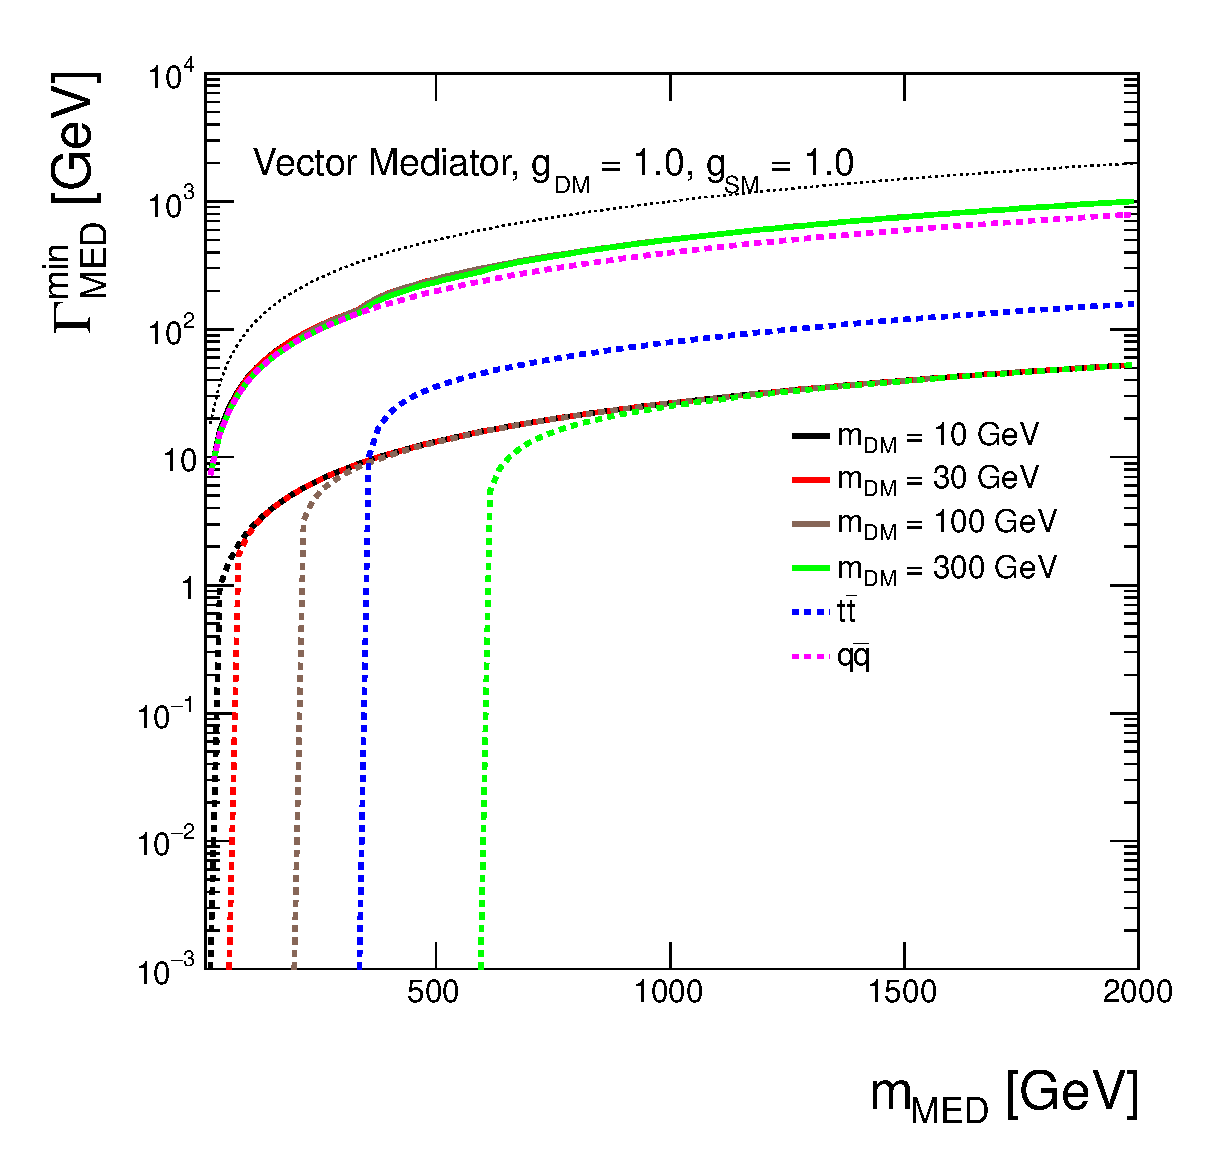
\includegraphics[width=0.95\textwidth]{figures/monojet/width_V.eps}
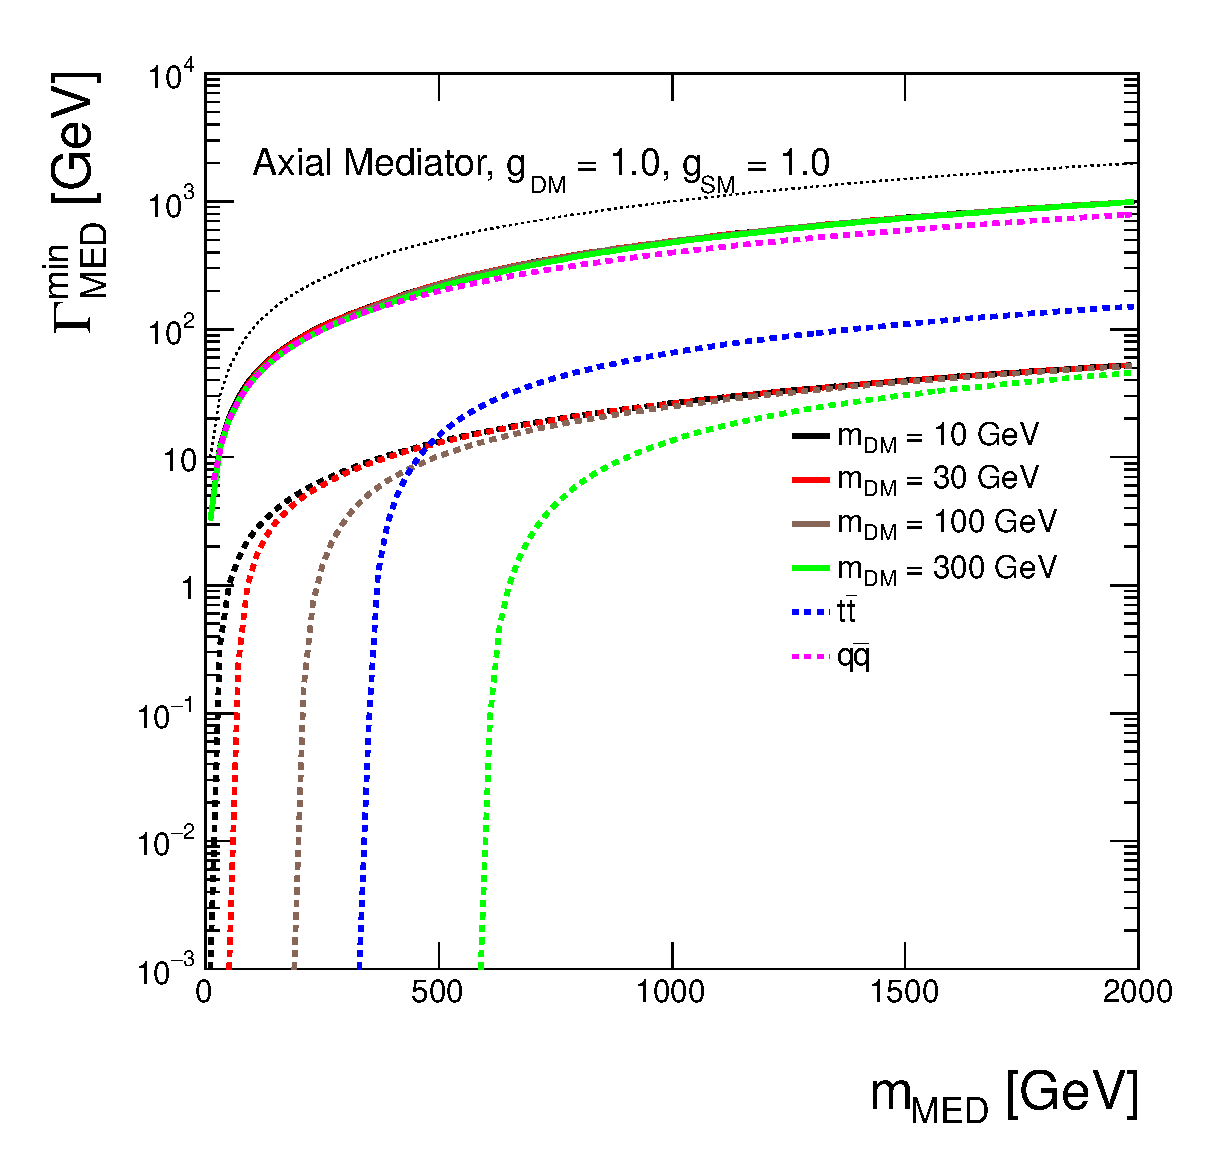
\includegraphics[width=0.95\textwidth]{figures/monojet/width_A.eps}
\caption{Minimal width as a function of mediator mass for vector and axial-vector mediator assuming couplings of 1. The total width is shown as solid lines for Dark Matter masses of 10~\gev, 30~\gev, 100~\gev and 300~\gev in black, red, brown and green, respectively. The individual contributions from Dark Matter are indicated by dotted lines with the same colors. The contribution from all quarks but top is shown as magenta dotted line and the contribution from top quarks only is illustrated by the dotted blue line. The dotted black line shows the extreme case $\Gamma_{\rm{min}}=\mMed$.}
\label{fig:monojet_width_V}
\end{figure}

Therefore, the minimal set of parameters under consideration for these two models is
\bea
\left\{ \mDM,~\mMed,~\gq, ~ \gDM\right\} \,.
\eea
See~\cite{Buchmueller:2014yoa} for a thorough discussion of these models.
 
%The two simplified models described here have four free parameters: mediator mass $\mMed$, Dark Matter mass $\mDM$, coupling of the mediator to quarks $\gq$ and coupling of the mediator to Dark Matter $\gDM$,


%%% new section by DS
\subsection{Spin structure of the couplings}
\label{sec:monojet_spin}

In this section, the differences between the vector and axial-vector models are described.
Furthermore, it is possible to consider other models in which mixed vector and axial-vector couplings are considered, for instance the couplings to the quarks are axial-vector whereas those to DM are vector. Such comparisons are also presented.

The samples with pure vector and pure axial-vector couplings are compared for $\mMed=100$~\gev and different Dark Matter masses in Fig.\,\ref{fig:monojet_VAmodels}. %The minimal width between the samples with the same Dark Matter and mediator masses differ only at the percent level.
No differences in the shape of the \MET distributions are observed between the samples with coincident masses. 
%\Todo{Do we want to propose to generate one model only and refer to the cross section tables in HEPData repository for the other?}
In the case of the on-shell Dark Matter pair production where $2\mDM\ll\mMed$, the cross sections of the pure vector and pure axial-vector models are similar. With increasing Dark Matter mass towards the $2\mDM=\mMed$ transition and beyond into the off-shell production regime, the relative difference between the cross sections of the two samples is increasing, with the vector samples having larger cross sections. 
%TODO \Todo{This can be understood in the eikonal approximation since the A terms have an additional $v^2$ in front.}

\begin{figure*}
\centering
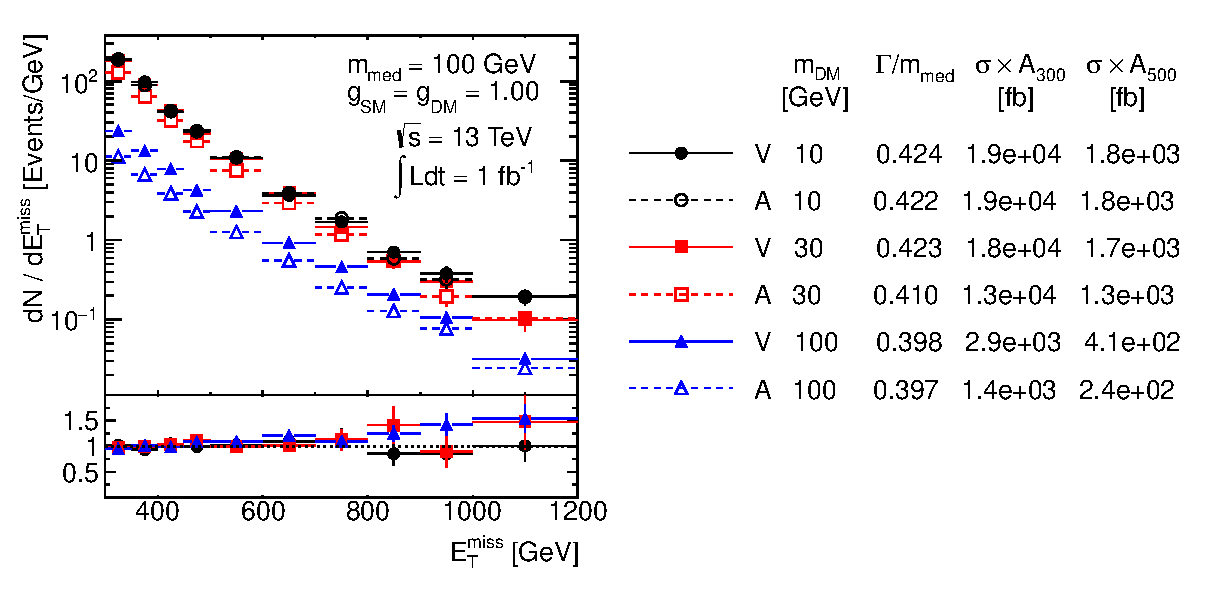
\includegraphics[width=0.95\textwidth]{figures/monojet/compareModels_VA_100.eps}
\caption[][-28pt]{Comparison of the pure vector and pure axial-vector couplings. The $\MET$ distribution is shown for the samples generated with $\mMed=100$~\gev and different Dark Matter masses. Ratios of the normalized distributions are shown for between the samples with coincident masses. $A_{300}$ and $A_{500}$ in the table denote the acceptance of the $\MET>300$~\gev and $\MET>500$~\gev cut, respectively.}
\label{fig:monojet_VAmodels}
\end{figure*}

Figure\,\ref{fig:monojet_scan_VA_mMed1000} shows the samples generated with pure and mixed couplings for $\mDM=100$~\gev and $\mMed=1\,\tev$, i.e. where the Dark Matter pair is produced on-shell. The mediator width between the pure vector and pure axial-vector couplings differ only by 2\% in this case, and $<10\%$ agreement between the cross sections is found. The mediator widths for the samples with the same type coupling to quarks agree at better than 1\% since the width is dominated by the quark contribution, as expected from
Eq.\,\ref{eq:monojet_min}.
%In the mediator rest frame, the angular distribution of the DM relative to the mediator direction of motion has the form $1+z^2+2*C*z$, where $z=\cos\theta$, with the second term only present in the mixed case, which may lead to acceptance differences.
No significant differences between the samples with same type Dark Matter coupling are seen, given the statistical precision of the generated samples. This is expected since the mediator is produced on-shell, and the details of the invisible decay are unimportant in cut-and-count searches.

For the off-shell Dark Matter pair production, shown in Fig.\,\ref{fig:monojet_scan_VA_mMed100} for $\mDM=100$~\gev and $\mMed=100$~\gev,
there is approximately a factor 2 difference
between the cross-sections of the samples with pure couplings is observed. As in the previous case, the samples with the same type coupling to Dark Matter are similar both in terms of cross sections and \MET shape. Since the contribution to the mediator width from Dark Matter is closed in this case, only the quark couplings define the width. Only couplings to light quarks are opened in the case of $\mMed=100$~\gev for which the differences between the partial widths of vector and axial-vector couplings are marginal. This explains the similar minimal widths for all four samples stated in Fig.\,\ref{fig:monojet_scan_VA_mMed100}.

In general, the coupling to quarks is not expected to play an important role as it is only needed to produce the mediator which is confirmed by the observations above. For scalar and psuedoscalar mediators, the coupling to Dark Matter determines the form of the matrix element which explains the similarity of the samples with the same type Dark Matter couplings. 
Based on these arguments, we recommend to consider only the models with pure vector couplings or pure axial-vector couplings.

\begin{figure*}
\centering
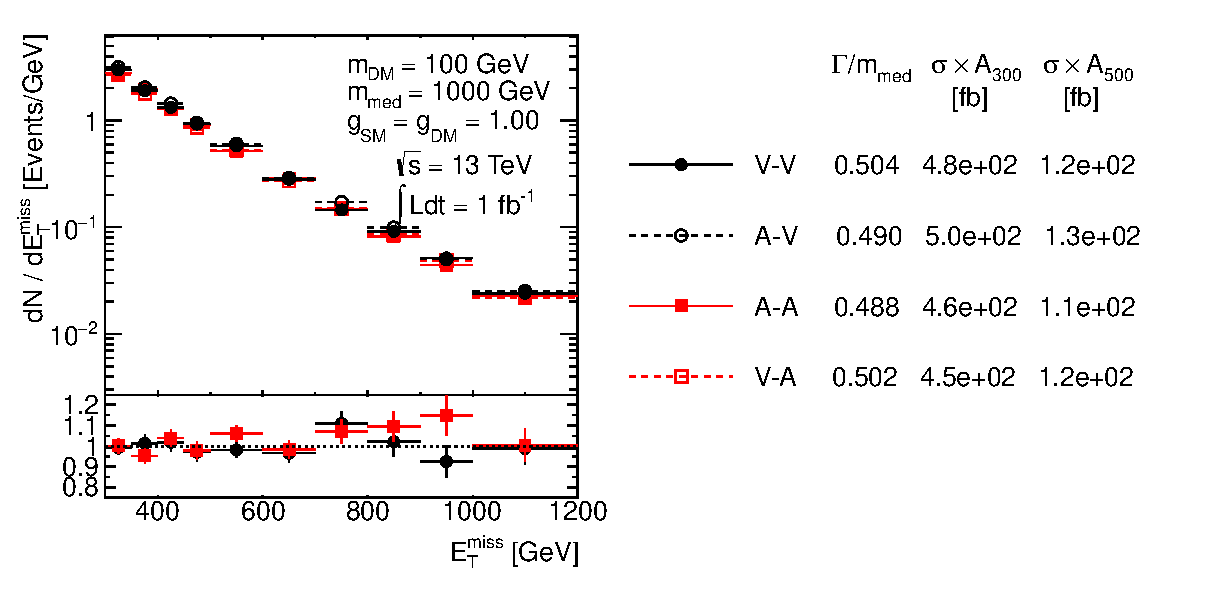
\includegraphics[width=0.95\textwidth]{figures/monojet/compareVA_100_1000.eps}
\caption[][-28pt]{Comparison of the pure vector, V-V, and pure axial-vector, A-A, couplings with mixed couplings, A-V and V-A where the first (second) letter indicates the Standard Model (Dark Sector) vertex. The $\MET$ distribution is shown for the samples generated with $\mDM=100$~\gev and $\mMed=1$~\tev. Ratios of the normalized distributions are shown for A-V over V-V and for V-A over A-A. $A_{300}$ and $A_{500}$ in the table denote the acceptance of the $\MET>300$~\gev and $\MET>500$~\gev cut, respectively.}
\label{fig:monojet_scan_VA_mMed1000}
\end{figure*}

\begin{figure*}
\centering
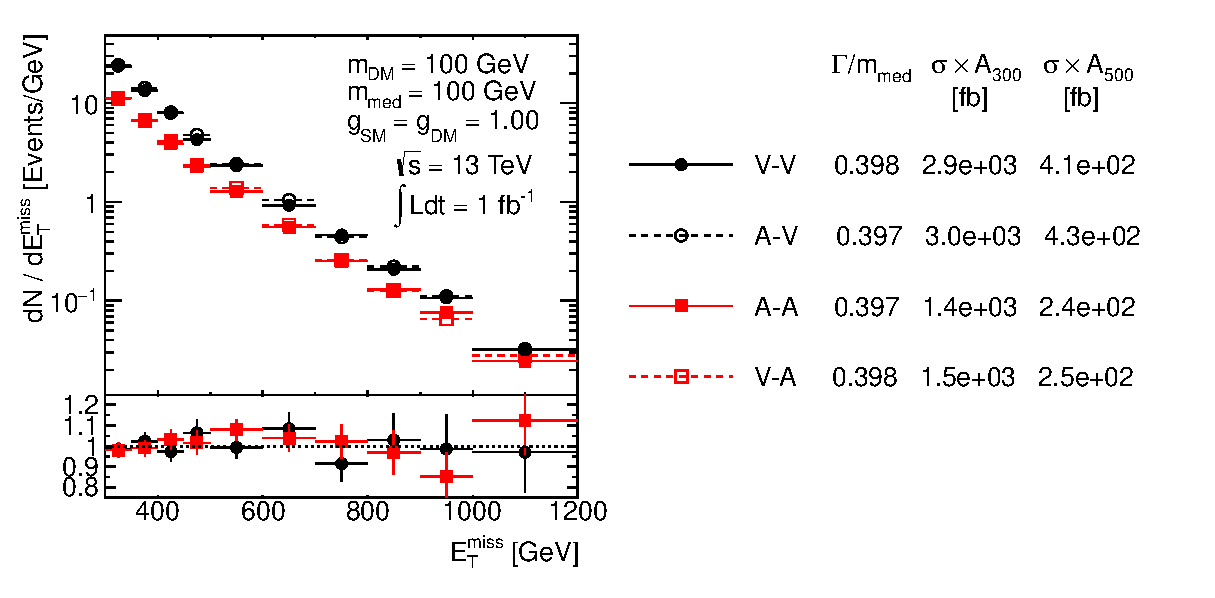
\includegraphics[width=0.95\textwidth]{figures/monojet/compareVA_100_100.eps}
\caption[][-28pt]{Comparison of the pure vector, V-V, and pure axial-vector, A-A, couplings with mixed couplings, A-V and V-A where the first (second) letter indicates the Standard Model (Dark Sector) vertex. The $\MET$ distribution is shown for the samples generated with $\mDM=100$~\gev and $\mMed=100$~\gev. Ratios of the normalized distributions are shown for A-V over V-V and for V-A over A-A. $A_{300}$ and $A_{500}$ in the table denote the acceptance of the $\MET>300$~\gev and $\MET>500$~\gev cut, respectively.}
\label{fig:monojet_scan_VA_mMed100}
\end{figure*}
%%% end of the new section by DS


\subsection{Parameter scan}
\label{sub:parameter_scan_monojet}

In order to determine an optimal choice of the parameter grid for the simulation of early Run-2 benchmark models, dependencies of the kinematic quantities and cross sections on the model parameters have been studied. The following paragraphs list the main observations from the scans over the parameters that support the final proposal for the benchmark signal grid.

\paragraph{Scan over the couplings}

To study the dependence of kinematic distributions on the coupling strength, samples were generated where a pair of $\mDM=10$~\gev Dark Matter particles is produced on-shell from the mediator of $\mMed=1$~\tev. 
Figure~\ref{fig:monojet_scan_V_g} compares the shapes of the \MET distribution for the different choices of the coupling strength. This is a generator-level prediction with no kinematic selections or detector simulation. Coupling values in the scan range 0.1--1.45, fixing $\gq=\gDM$, correspond to a rough estimate of the lower sensitivity of mono-jet analyses and a maximum coupling value such that $\Gamma_{\rm{min}} < \mMed$. We observe that the shapes of the \MET or jet \pT distributions do not depend on the couplings (and consequently the width) in the ranges considered. A large width of the mediator implies a broad integral over the contributing parton distributions, which might not be well approximated by the midpoint of this integral.  This study shows that the effect, in the \pT distribution of the observed gluon, is not important.

Based on similar findings for different choices of
\mMed and \mDM, we conclude that the shapes of
kinematic distributions are not altered
by coupling variations, neither for the on-shell Dark Matter production where $\mMed>2\mDM$,
nor for the off-shell Dark Matter production where $\mMed<2\mDM$. Only the production cross sections change.
Differences in kinematic distributions are expected only close to the transition region where both on-shell and off-shell decays occur.
%TODO clarify slide 9 and 10 in https://indico.cern.ch/event/389275/contribution/1/material/slides/0.pdf
%TODO check explicitly for V and A (generate corresponding samples)
\begin{figure*}
\centering
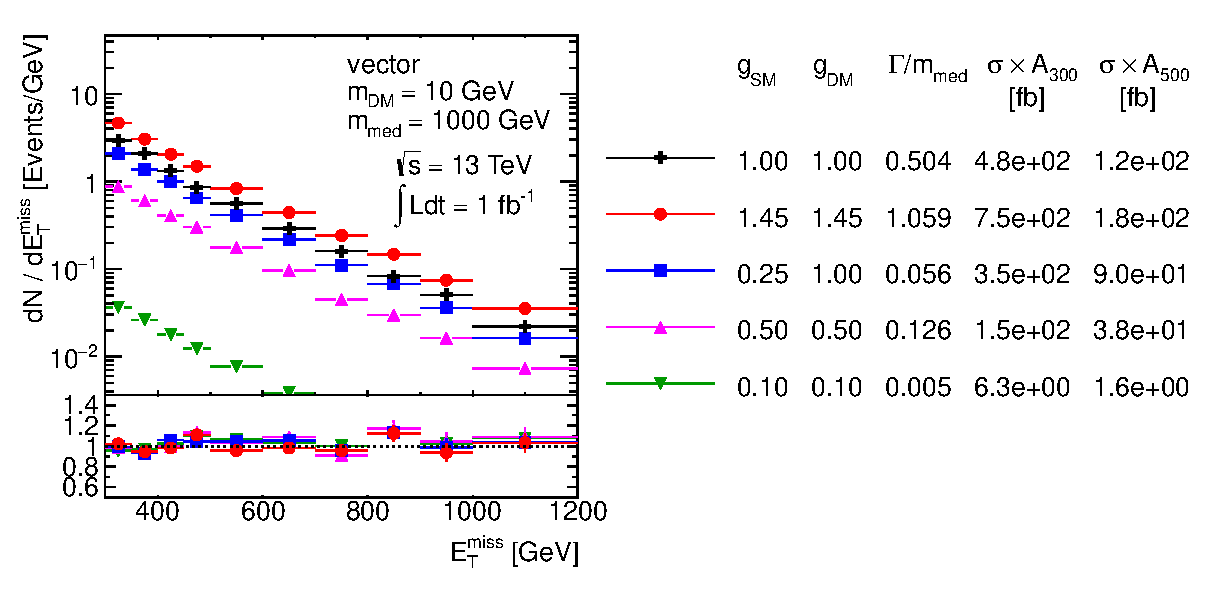
\includegraphics[width=0.95\textwidth]{figures/monojet/scan_g_V_10_1000.eps}
\caption[][-28pt]{Scan over couplings. The $\MET$ distribution is compared for the vector mediator models using the parameters as indicated. Ratios of the normalized distributions with respect to the first one are shown. $A_{300}$ and $A_{500}$ in the table denote the acceptance of the $\MET>300$~\gev and $\MET>500$~\gev cut, respectively.}
\label{fig:monojet_scan_V_g}
\end{figure*}

%When small coupling strengths are combined with extremely heavy mediators, one must take particular care to integrate over all values of the dark matter pair invariant mass, down to the lowest values for which the \MET satisfies threshold requirements. See the Appendix \ref{sec:monojet_implementation} page \pageref{thought:heavynarrowmediators} for details.

Special care needs to be taken when coupling strengths are combined with extremely heavy mediators.
Figure\,\ref{fig:monojet_narrow} suggests a change in the shape of the
\MET distribution for a $\mMed=5$~\tev mediator
once $\Gamma_{\rm{min}}/\mMed$ is of the order of a percent or lower.
Such heavy mediators, although inacessible by the LHC data, are interesting since they provide a good approximation for benchmark EFT models.
The observed difference among the simplified models in the plot arises from the fact that the region of low invariant masses of the Dark Matter pair, $m_{\bar{\chiDM}\chiDM}$, is suppressed due to narrow Breit-Wigner peak that only probes a narrow window of parton distribution functions. For wider mediators, the low mass region is significantly enhanced by parton distribution functions at low Bjorken $x$, as illustrated in Fig.\,\ref{fig:monojet_mchichi}(a).
This explains why the sample with the narrowest mediator in Fig.\,\ref{fig:monojet_narrow} is heavily suppressed in terms of production cross section and also gives different \MET shape.
%In general, for such extreme parameter choices the EFT model should give the correct answer.
Furthermore, Fig.\,\ref{fig:monojet_narrow} compares the vector model with 5~\tev mediator to the D5 EFT sample and reveals that the simplified models with larger mediator widths (e.g. for couplings of 1 where $\Gamma_{\rm{min}}/\mMed\sim0.5$) are the ones resembling the kinematics of contact interactions. This is because the production in the EFT model is always off-shell, i.e. no peak in the $m_{\bar{\chiDM}\chiDM}$ distribution is present.
In case of narrow width mediators, e.g. $\Gamma_{\rm{min}}/\mMed\sim0.05$, even larger mediator masses need to be chosen in order to significantly suppress the peak in the $m_{\bar{\chiDM}\chiDM}$ distribution and reproduce the kinematic shapes of an EFT model. Figure\,\ref{fig:monojet_mchichi}(b) verifies that the choice of 10~\tev mediator mass is sufficient to achieve that.


%\Todo{Refer to results of ongoing study in Section 6.}
%CD: commented out, we have to ask for having 7 TeV mediators
% In case the simplified model calculation does not reproduce the EFT result, the phase space generation of the simplified model has to be carefully examined in order to understand the cause of the problem. Fortunately, this is a rather academic discussion as such extreme corners of the parameter space are not going to be considered for presentation of Run-2 results.

%Uli: as fabio says, increasing bwcutoff might improve things in the case you are considering
%
%for a mediator with mass M = 7~\tev and width Gamma = 36~\gev, i think the correct way to do this calculation is to work in an EFT; this should give you the correct result
%
%in fact, if your simplified model calculation does not reproduce the EFT result for such extreme parameter choices, you have to carefully look at the phase-space generation of the simplified model calculation (as you did). at the end you probably have to tailor the phase-space generator of \madgraph, \powheg, etc. to get it right; this will be non-trivial since phase-space generation is an art! furthermore, one has to do this process 
%by process and the difficulties will increase from mono-jet to ttbar + \MET, etc. 

%\begin{figure}
%\centering
%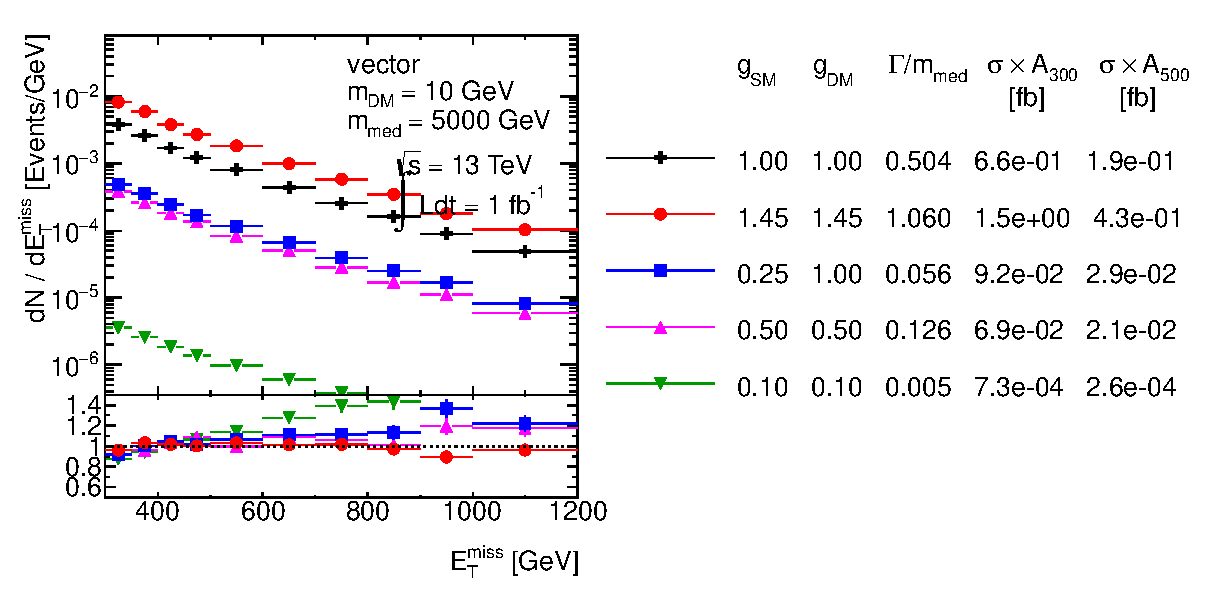
\includegraphics[width=0.95\textwidth]{figures/monojet/scan_g_V_10_5000.eps}
%\caption{Scan over couplings. The $\MET$ distribution is compared for the vector mediator models using the parameters as indicated. Ratios of the normalized distributions with respect to the first one are shown. $A_{300}$ and $A_{500}$ in the table denote the acceptance of the $\MET>300$~\gev and $\MET>500$~\gev cut, respectively.}
%\label{fig:monojet_narrow}
%\end{figure}

\begin{figure*}
\centering
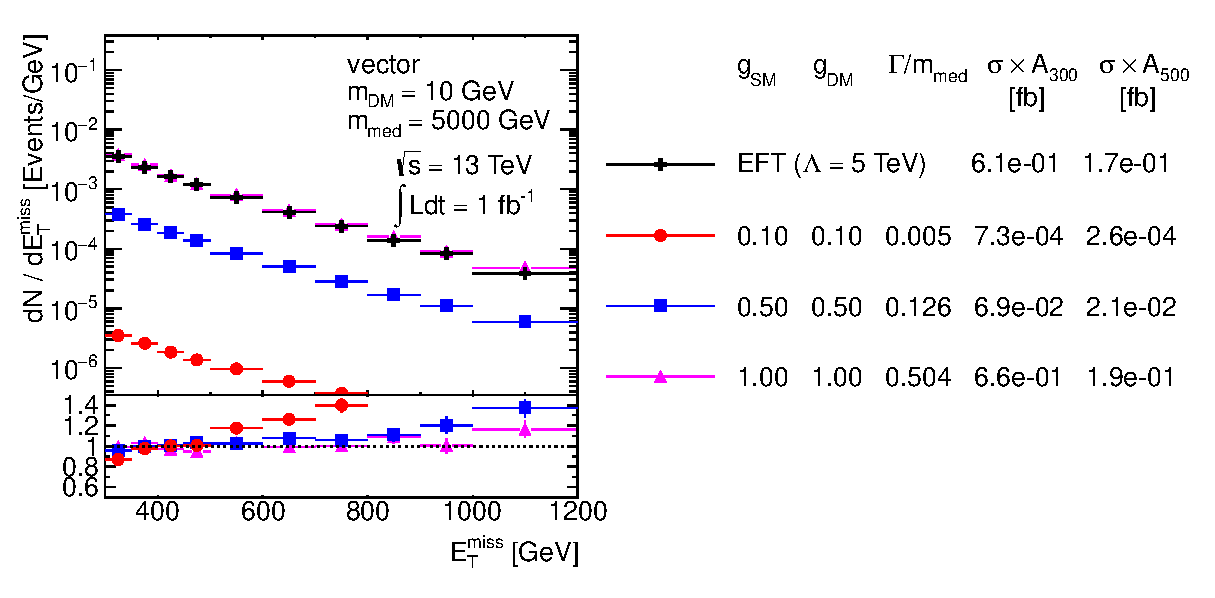
\includegraphics[width=0.95\textwidth]{figures/monojet/scan_g_EFT_10_5000.eps}
\caption[][-28pt]{Comparison of the $\MET$ distributions from the D5 EFT sample and the vector models with 5~\tev heavy mediator of various widths. Ratios of the normalized distributions with respect to the first one are shown. $A_{300}$ and $A_{500}$ in the table denote the acceptance of the $\MET>300$~\gev and $\MET>500$~\gev cut, respectively.}
\label{fig:monojet_narrow}
\end{figure*}

\begin{figure}
\centering
\subfloat[]{
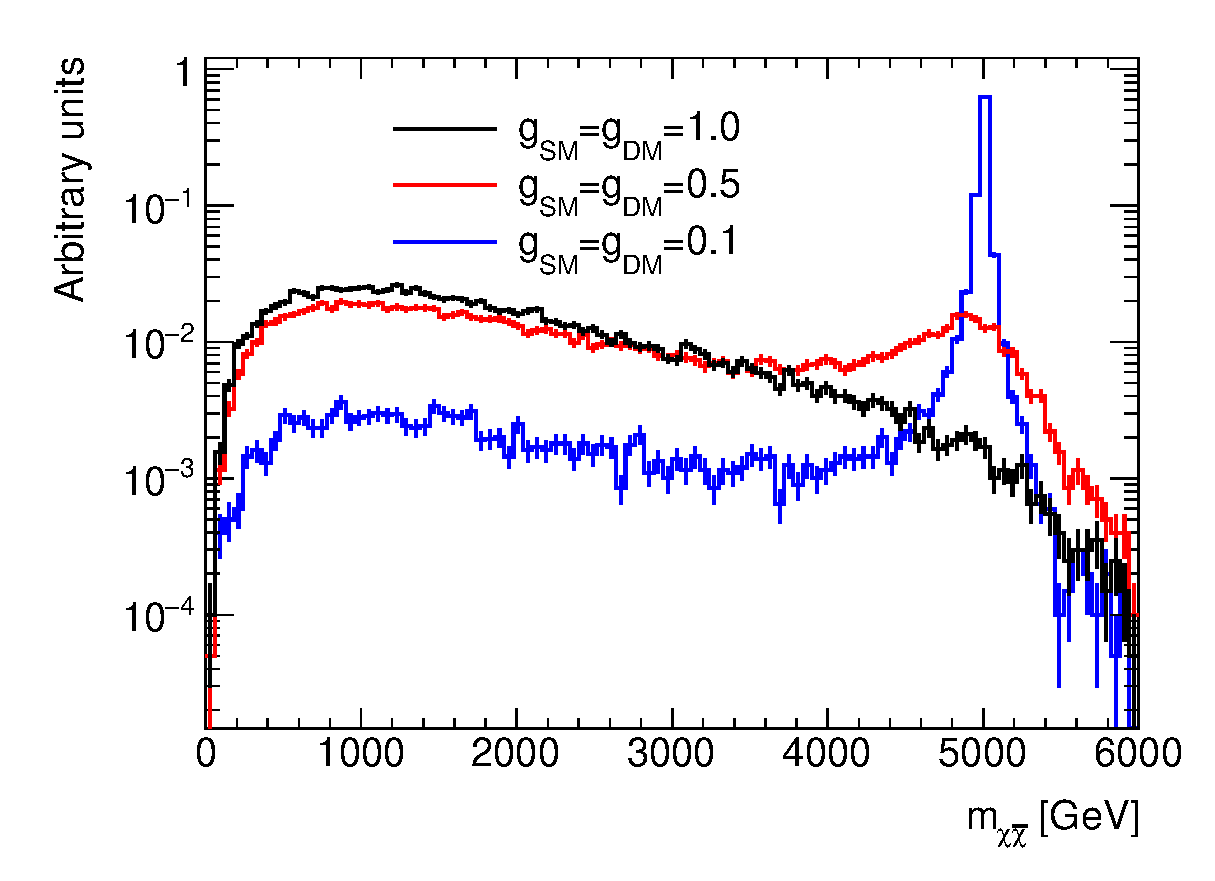
\includegraphics[width=0.8\textwidth]{figures/monojet/mxx.eps}% width = 0.73 => regular textwidth of figure environment. figure* used to avoid overlapping captions.
\label{fig:monojet_mchichi_a}}
\hfill
\subfloat[]{
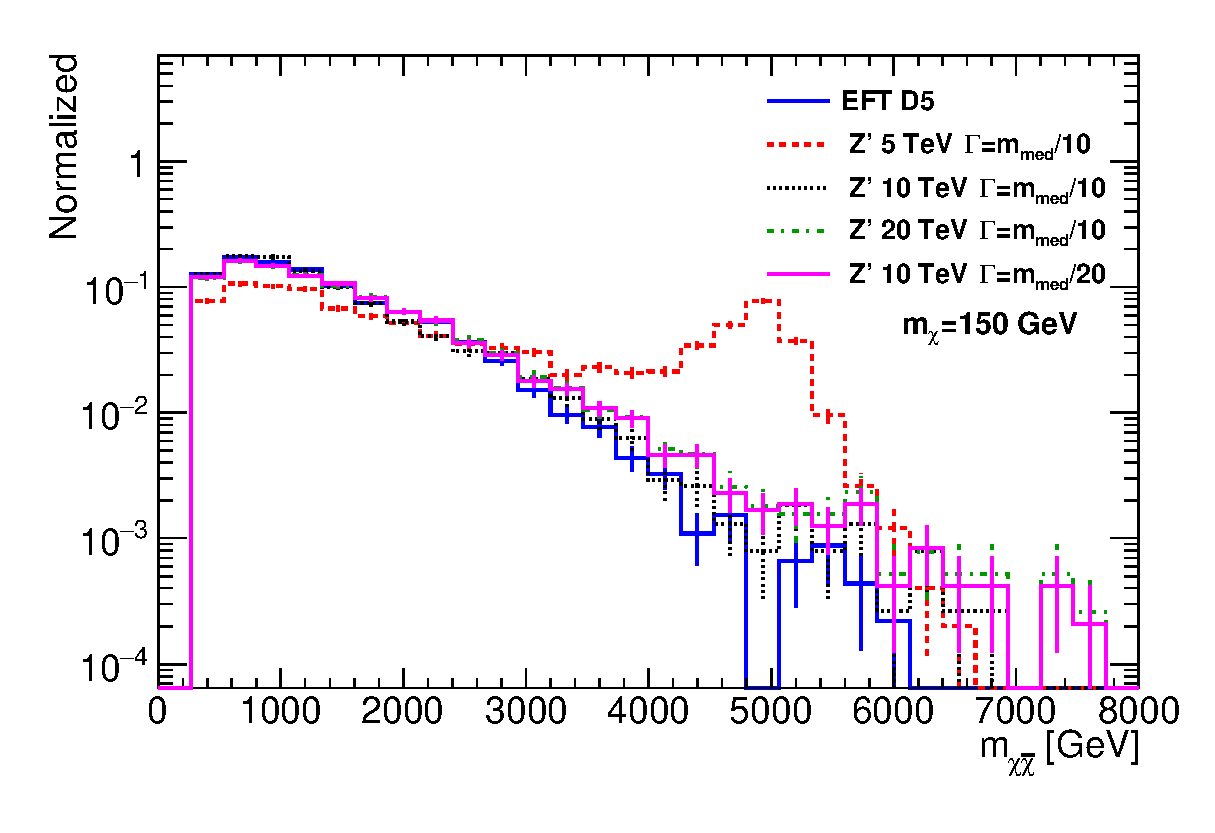
\includegraphics[width=0.8\textwidth]{figures/EFT/TruthShat3_compEFTvsZprime_DM150_narrow_new.eps}
\label{fig:monojet_mchichi_b}}
\caption[][14pt]{Invariant mass of the Dark Matter pair in the vector mediator samples with $\mDM=10$~\gev, $\mMed=5$~\tev and different coupling strengths (a).
Similar comparison is shown for the samples with different mediator masses considering $\Gamma_{\rm{min}}/\mMed=0.05$ and $0.1$ (b).
An EFT sample is also displayed in the latter case. The distributions are normalised to unit area.}
\label{fig:monojet_mchichi}
\end{figure}


Since kinematic distributions are robust to
changes in the specific values of coupling as long as heavy narrow mediators are generated correctly (see Appendix~\ref{thought:heavynarrowmediators} for discussion), 
the choice of $\gq=\gDM$ is reasonable 
to reduce the parameter space to be scanned. 
There are no complications associated
with small couplings, but, also, the early part of Run~2 will not be
sensitive to them.  The range of couplings we recommend limit the
calculated width of the mediator to be near or below \mMed.

For direct mediator searches, such as $q\bar q\to Z^\prime \to q\bar q$, asymmetric couplings ($\gq \ne \gDM$)
might also be considered. A scan in \gDM vs \gq can then be performed for a fixed mediator mass. Such searches
%such as those for
%dijet resonances,
may restrict \gq to a greater degree than
\gDM.

\paragraph{Scan over \mDM}

For a fixed mediator mass \mMed and couplings, the Dark Matter mass falls into three regimes:
\begin{itemize}
\item[On-shell:] When $\Mmed \gg 2 \mDM$, most mediators are produced on-shell. The hardness of the ISR is set by \Mmed, and the kinematic distributions do not strongly depend on \mDM. This is illustrated in Fig.~\ref{fig:monojet_scan_V_mDM1000} for an example of \mMed=1~\tev 10~\gev $<\mDM<$ 300~\gev. The cross section decreases as the \mDM approaches $\mMed/2$. A coarse binning along $\mDM$ is sufficient.
\item[Threshold:] When $\Mmed \approx 2\mDM$, the production is resonantly enhanced, and both the cross section and kinematic distributions change more rapidly as a function of the two masses, and finer binning is needed in order to capture the changes.
\item[Off-shell:] When $\Mmed \ll 2 \mDM$, the Dark Matter pair is produced off-shell. The mediator propagator gives an explicit suppression of $(\Mmed/Q)^4$ that suppresses hard ISR. The $\mDM=1$~\tev case, shown in Fig.~\ref{fig:monojet_scan_V_mDM1000}, and Figure\,\ref{fig:monojet_scan_V_mDM100} demonstrates that the \MET spectrum hardens with increasing \mDM, accompanied by the gradual decrease of the cross section. Due to the significant cross section suppression, it is not necessary to fully populate the parameter space. Imminent LHC searches are not expected to be sensitive to these signals.
\end{itemize}

\begin{figure*}
\centering
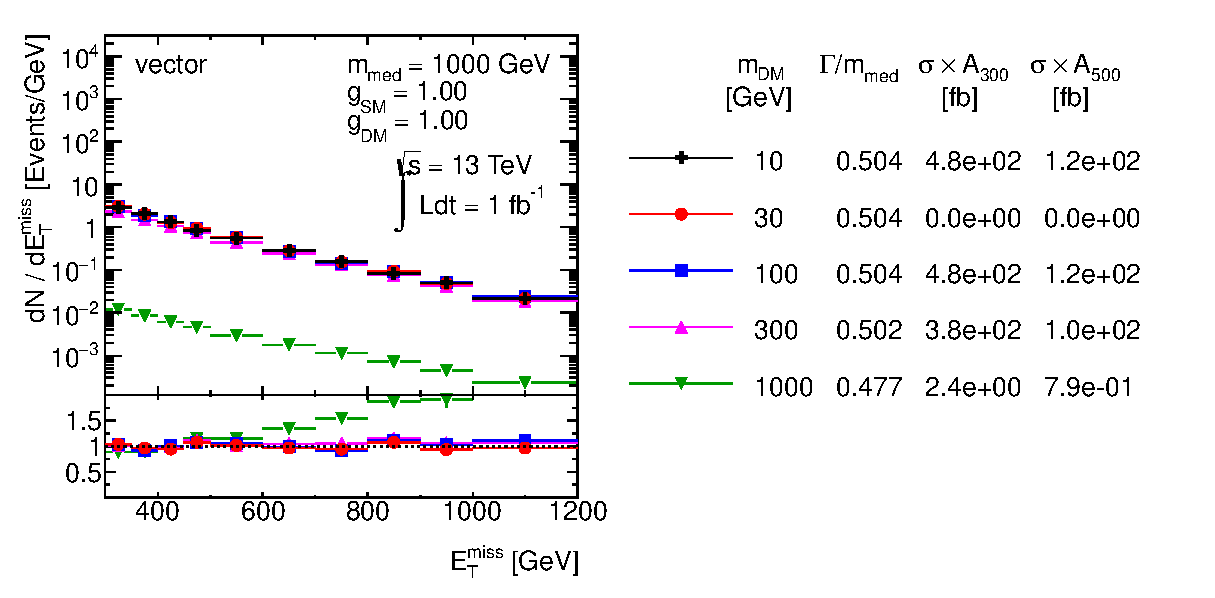
\includegraphics[width=0.95\textwidth]{figures/monojet/scan_mDM_V_1000.eps}
\vspace{4\baselineskip}
\caption[][-84pt]{Scan over Dark Matter mass. The $\MET$ distribution is compared for the vector mediator models using the parameters as indicated. Ratios of the normalized distributions with respect to the first one are shown. $A_{300}$ and $A_{500}$ in the table denote the acceptance of the $\MET>300$~\gev and $\MET>500$~\gev cut, respectively.}
\label{fig:monojet_scan_V_mDM1000}
\end{figure*}

\begin{figure*}
\centering
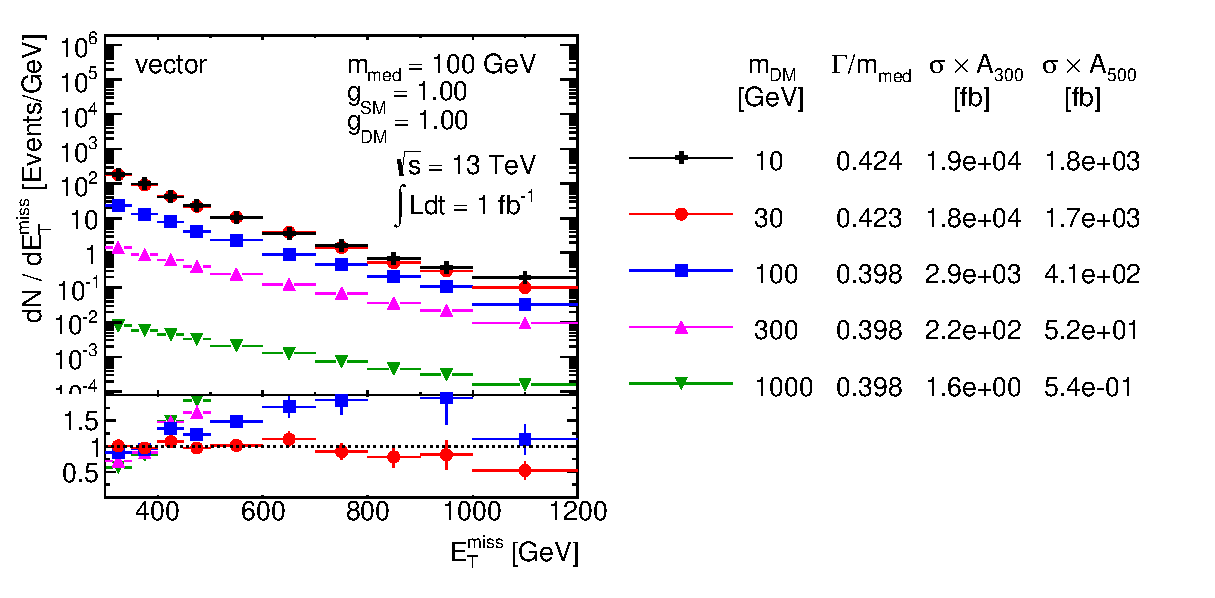
\includegraphics[width=0.95\textwidth]{figures/monojet/scan_mDM_V_100.eps}
\vspace{4\baselineskip}
\caption[][-84pt]{Scan over Dark Matter mass. The $\MET$ distribution is compared for the vector mediator models using the parameters as indicated. Ratios of the normalized distributions with respect to the first one are shown. $A_{300}$ and $A_{500}$ in the table denote the acceptance of the $\MET>300$~\gev and $\MET>500$~\gev cut, respectively.}
\label{fig:monojet_scan_V_mDM100}
\end{figure*}

\paragraph{Scan over the mediator mass}

Changing the mediator mass for fixed Dark Matter mass and couplings leads to significant differences in cross section and shapes of the kinematic variables for on-shell production, as shown in Fig.\,\ref{fig:monojet_scan_V_mMed10}. As expected, higher mediator masses lead to harder $\MET$ spectra.
On the other hand, the $\MET$ shapes are similar in the off-shell Dark Matter production regime.  This
is illustrated in Fig.\,\ref{fig:monojet_scan_V_mMed1000}. Therefore, a coarse binning in \mMed is sufficient in the off-shell regime.

\begin{figure*}
\centering
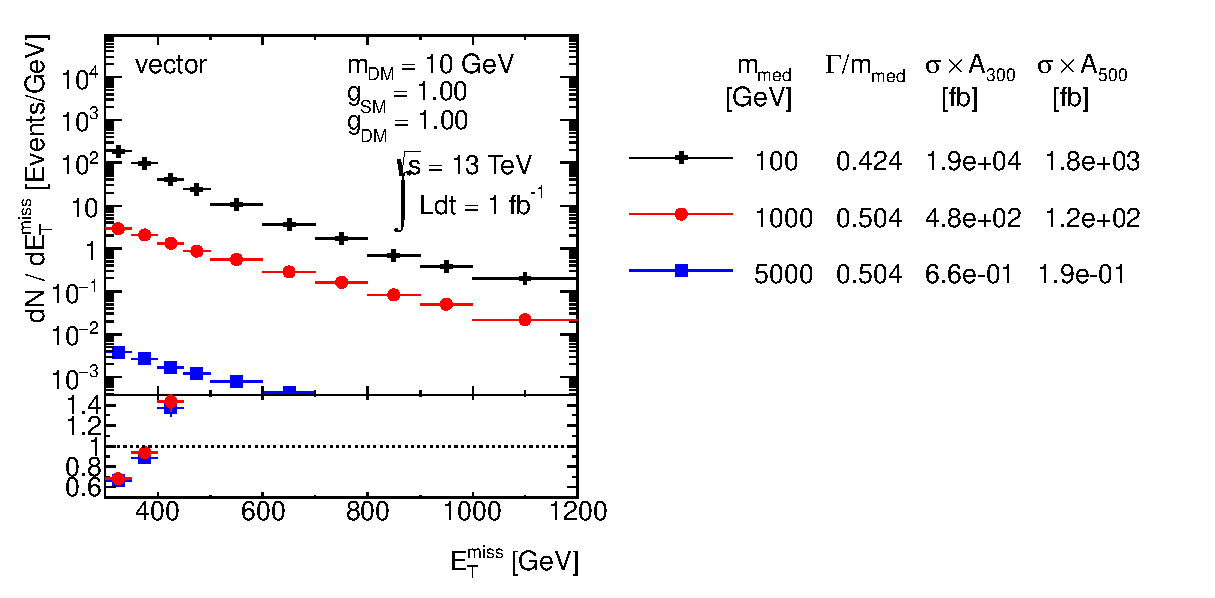
\includegraphics[width=0.95\textwidth]{figures/monojet/scan_mMed_V_10.eps}
\vspace{4\baselineskip}
\caption[][-84pt]{Scan over mediator mass. The $\MET$ distribution is compared for the vector mediator models using the parameters as indicated. Ratios of the normalized distributions with respect to the first one are shown. $A_{300}$ and $A_{500}$ in the table denote the acceptance of the $\MET>300$~\gev and $\MET>500$~\gev cut, respectively.}
\label{fig:monojet_scan_V_mMed10}
\end{figure*}

\begin{figure*}
\centering
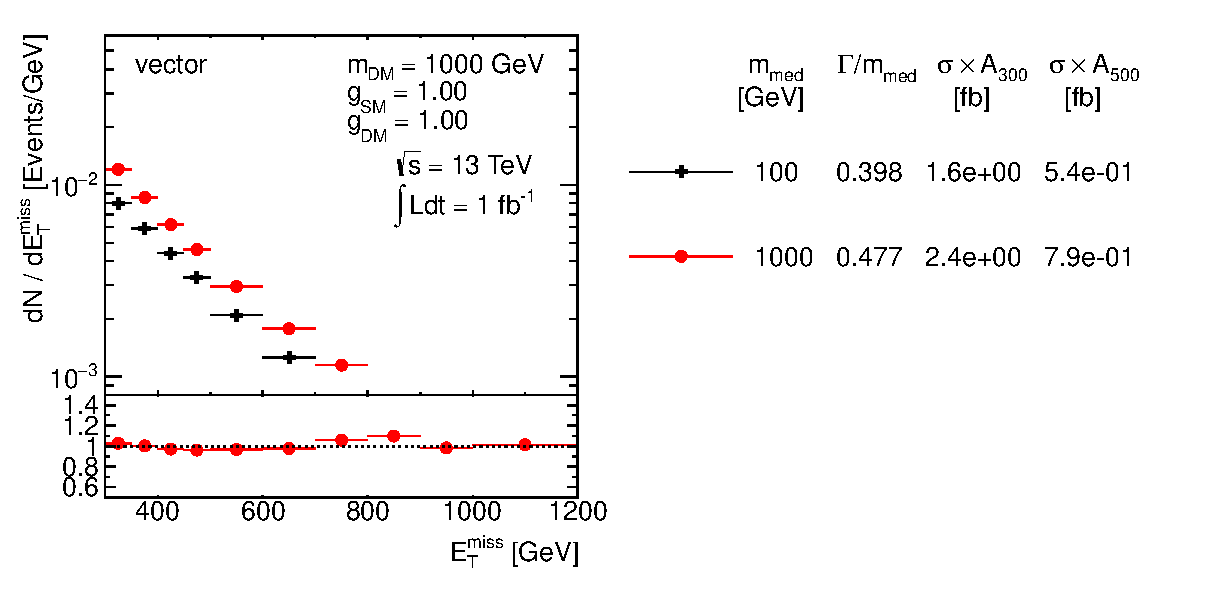
\includegraphics[width=0.95\textwidth]{figures/monojet/scan_mMed_V_1000.eps}
\caption[][-28pt]{Scan over mediator mass. The $\MET$ distribution is compared for the vector mediator models using the parameters as indicated. Ratios of the normalized distributions with respect to the first one are shown. $A_{300}$ and $A_{500}$ in the table denote the acceptance of the $\MET>300$~\gev and $\MET>500$~\gev cut, respectively.}
\label{fig:monojet_scan_V_mMed1000}
\end{figure*}

\paragraph{Proposed parameter grid}

The final step in proposing a parameter grid is to evaluate the sensitivity
of Run-2 LHC data with respect to rate and/or kinematics.
%In order to motivate the highest mediator mass grid point, the expected sensitivity of Run-2 LHC data needs to be taken into account.
The parameter scan focuses on two important regions, the light mediator region and  the heavy mediator limit to reproduce the EFT limit, 
and takes into account the projected sensitivities for the mono-jet analysis.

Considering simplified models also allows to discuss constraints from different search channels. In the case of the \schannel exchange, the results from the mono-jet final states, where the mediator decays to a DM pair, one can also take into account dijet constraints on the processes where the mediator decays back to Standard Model particles. The importance of the dijet results depend on the magnitude of the coupling $\gq$. We recommend to keep the two channels rather independent by choosing $\gq=0.25$ and $\gDM=1$, based on the findings given in Ref.\,\cite{Chala:2015ama}. Furthermore, it is also important to mention this choice leads to $\Gamma_{\rm{min}}/\mMed \lsim 0.06$. Note that the usual choice of $\gq=\gDM=1$ used in literature leads to $\Gamma_{\rm{min}}/\mMed \sim 0.5$, which makes the applicability of the narrow with approximation questionable.

Projected sensitivities for a 14~\tev\, mono-jet analysis are available from ATLAS~\cite{ATL-PHYS-PUB-2014-007}. The expected upper limit at 95\% confidence level on the product of cross section, acceptance and efficiency, $\sigma\times A\times\epsilon$, in the final Run-1 ATLAS mono-jet analysis\,\cite{Aad:2015zva} is 51\,fb and 7.2\,fb  for $\MET>300$~\gev and $\MET>500$~\gev, respectively. ATLAS estimates a factor of two increase in sensitivity with the 2015 data. Given that cross section for $V+$jets processes increases by roughly a factor 2 %\Todo{Can we get more precise number and a citation? Is this in Sarah's V+jets paper?} 
when going from $\sqrt{s}=8$~\tev to 13~\tev, similar fiducial cross section limits can be expected with the first Run-2 data as from the final Run-1 analysis.
The generator level cross section times the acceptance at $\MET>500$~\gev for the model with couplings $\gq=0.25$ and $\gDM=1$, a light Dark Matter particle of
\mDM=10~\gev and a \mMed=1~\tev vector mediator is at the order of 100\,fb, i.e. the early Run-2 mono-jet analysis is going to be sensitive to heavier mediators than this. The value of $\sigma\times A$ at $\MET>500$~\gev for 5~\tev vector mediator is at the order of 0.1\,fb, therefore this model lies beyond the reach of the LHC in the early Run 2. However, models with high enough mediators are still useful to reproduce the EFT result.

Following these arguments, \mMed grid points are chosen, roughly equidistant in a logarithmic scale: 10~\gev, 20~\gev, 50~\gev,  100~\gev, 200~\gev, 300~\gev, 500~\gev, 1000~\gev and 2000~\gev. In the threshold regime $\mMed=2\mDM$, the $\mDM$ grid points are taken at approximately $\mMed/2$, namely: 10~\gev, 50~\gev, 150~\gev, 500~\gev and 1000~\gev. Points on the on-shell diagonal are always chosen to be 5~\gev away from the threshold, to avoid numerical instabilities in the event generation. 
The detailed studies of the impact of the parameter changes on the cross section and kinematic distributions presented earlier in this section support removing some of the grid points and relying on interpolation. The optimized grids proposed for the vector and axial-vector mediators are given in Table.\,\ref{tab:mDMmMedScan_VA}.
% containing 36
%29 
%mass points each. 
One point at very high mediator mass (10~\tev) is added for each of the DM masses scanned, to aid the reinterpretation of results in terms of contact interaction operators (EFTs), as discussed in Section~\ref{sec:RecommendationEFTResults}. 

% \begin{figure}
% \centering
% 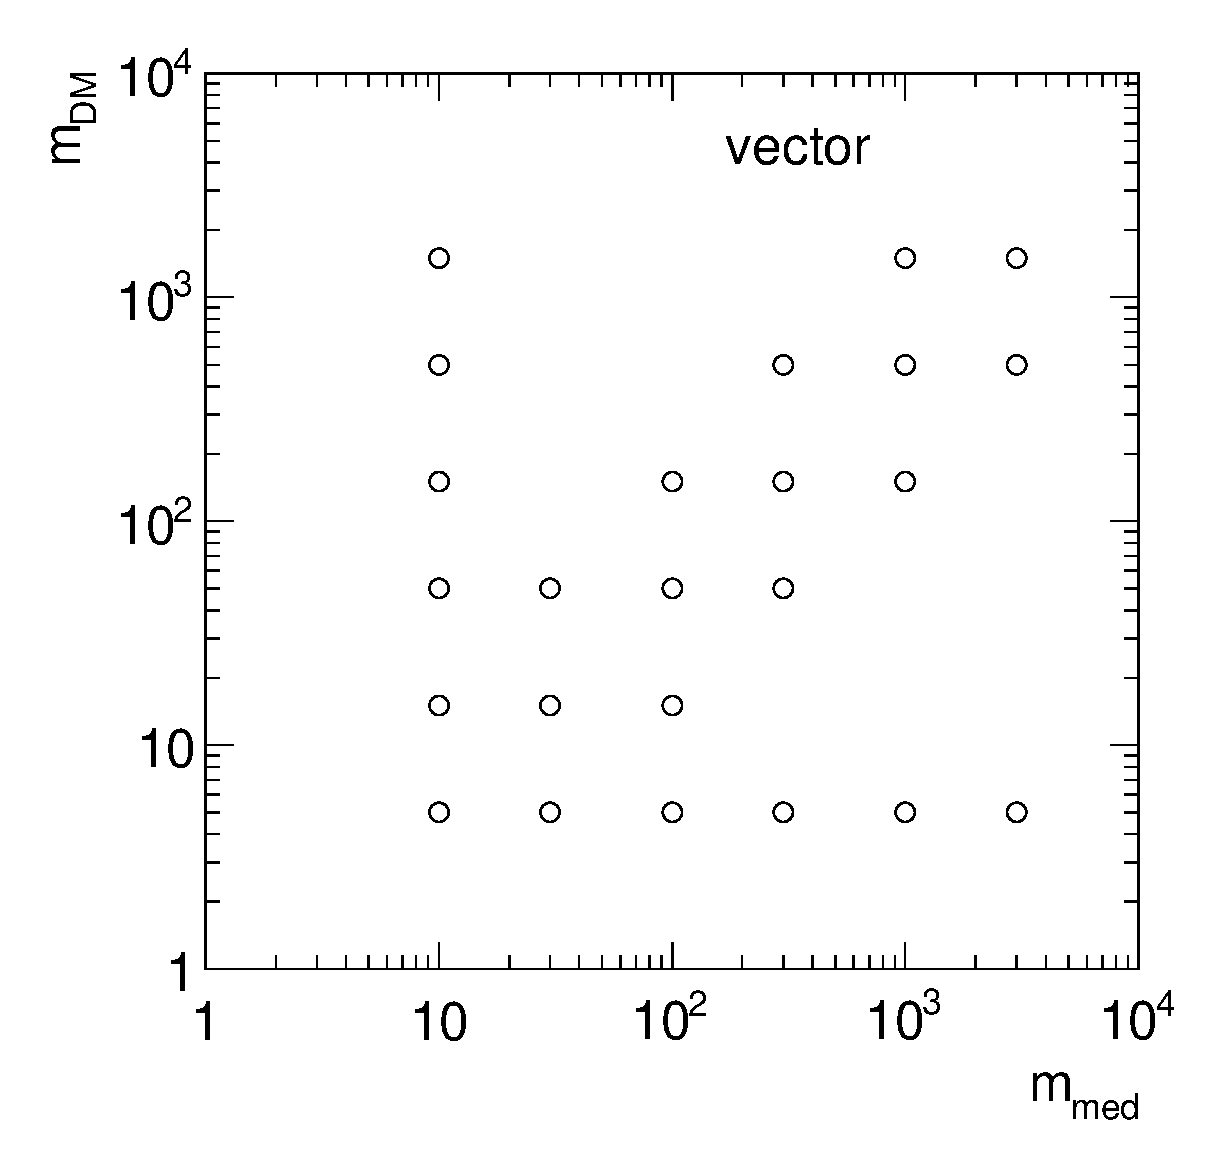
\includegraphics[width=0.95\textwidth]{figures/monojet/grid_V.eps}
% 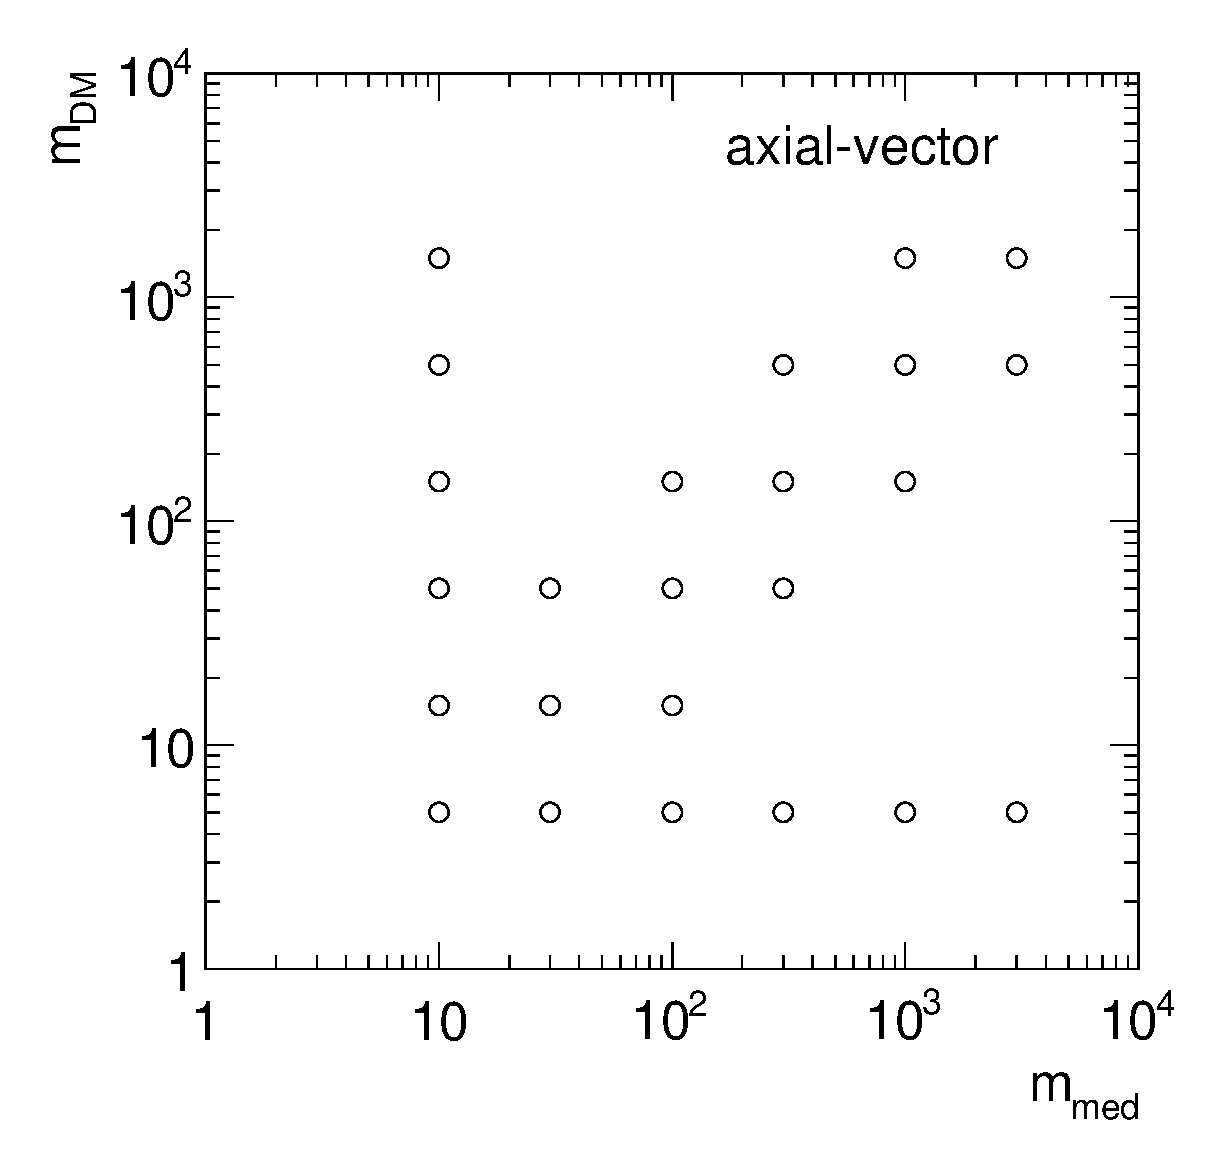
\includegraphics[width=0.95\textwidth]{figures/monojet/grid_A.eps}
% \caption{Proposed parameter grid for vector and axial-vector mediator in the $\mMed$--$\mDM$ plane.}
% \label{fig:monojet_grid_V}
% \end{figure}

\begin{table}[!h]
\centering
\resizebox{\textwidth}{!}{
\begin{tabular}{| l |r r r r r r r r r r|}
\hline
\multicolumn{1}{|c|}{\mDM/\gev} & \multicolumn{10}{c|}{\mmed/\gev} \\
\hline
 1             &         10  & 20 & 50 & 100 & 200 & 300 & 500 &         1000  &                 2000   &         10000  \\
 10   	       &         10  & 15 & 50 & 100 &     &     &     &               &                        &     10000      \\
 50            &   10  & 
& 50 &  95 & 200 & 300 &     &               &                        &    10000       \\
 150           &         10  &    &    &     & 200 & 295 & 500 &    1000    &                  &     10000      \\
 500           &         10  &    &    &     &     &     & 500 &          995  &                 2000   &     10000      \\
 1000          &         10  &    &    &     &     &     &     &         1000  &                 1995   &         10000  \\
\hline
\end{tabular}
}
\caption{Simplified model benchmarks for \schannel simplified models (\spinone mediators 
decaying to Dirac DM fermions in the V and A case, taking the minimum width for \gq = 0.25 and \gDM = 1)}.
% Points in \textbf{bold} are only generated for the vector/axial vector cases, while points in 
% \textit{italics} are generated for the monojet analysis 
% but not for the search including heavy quarks. This table corresponds to 29 points for monojet vector/axial vector models,
% 26 points for monojet scalar/pseudoscalar models and 24 points for $t \bar{t}$+\MET scalar/pseudoscalar models.}

\label{tab:mDMmMedScan_VA}
% \end{sidewaystable}
\end{table}

The presentation of the results in the $\gq$--$\gDM$ plane for fixed masses benefits from cross section scaling and is discussed in Section\,\ref{sec:monojet_scaling}.

%% It is difficult to visualize a four dimensional scan.
%% However, it is convenient to study the parameter dependence,
%% and present results, in two projections:
%% (a) the $\mMed$--$\mDM$ plane for a particular choice of the couplings, and\\
%% (b) the $\gq$--$\gDM$ plane for a particular choice of the masses.

%% %discuss expected sensitivity (cite PUB note) when motivating mDM and mMed range
%% %motivate the mass point for the coupilng scan

%% We choose to display the results in the $\mMed$--$\mDM$ plane for the choice of the couplings $\gq=\gDM=1$. 

\subsection{Additional considerations for $V$+\MET{} signatures}
\label{sec:bosonrad}
\svnidlong
{$HeadURL: $}
{$LastChangedDate: $}
{$LastChangedRevision: $}
{$LastChangedBy: $}
\svnid{$Id: $}   

All models detailed in this Section are applicable to signatures where 
 a photon, a W boson, a Z boson or a Higgs boson
 is radiated from the initial state partons instead of a gluon. 
The experimental signature is identified as \textit{V+\MET} and it
has been studied in Refs.~\cite{}.

\Todo{Add experimental citations.}
\Todo{Add link to section describing EW bosons from a blob. CD: why here?}

Monojet searches are generally more sensitive
with respect to final states including bosons, due to the much
larger rates of signal events featuring quark or gluon radiation with
respect to radiation of bosons~\cite{Zhou:2013fla},
in combination with the low branching ratios if leptons from
boson decays are required in the final state.
The rates for the Higgs boson radiation is too low for these models
to be considered a viable benchmark~\cite{Carpenter:2013xra}.
However, the presence of photons,
leptons from W and Z decays,
and W or Z bosons decaying hadronically
allow backgrounds to be rejected more effectively,
making Z/gamma/W+\MET searches
still worth comparing with searches in the jet+\MET final state.

%\Todo{Additional motivations exist for this final state from SUSY searches.}
%TODO: Linda is writing sentence to make this stronger. 

% The three commonly chosen EFT benchmarks for Dirac dark matter that are
% kinematically distinct for what concerns the observables used in
% \MET+X searches~\footnote{[CD: we would need a plot here, or a reference to
% monojet section where this is shown]} and span a wide range of \MET spectrum in
% the boson+\MET searches are, in the notation of ~\cite{Goodman:2010ku},
% the D1 (scalar SM/WIMP interaction), D5 (vector-vector interaction) and D9
% (tensor interaction) operator.

In the case of a spin-1 mediator,
an example Feynman diagram for these processes can be constructed by taking
Fig.~\ref{fig:OP} and replacing the gluon with $\gamma,W$ or $Z$.
The interest for searches with W bosons in the final state
has been elevated by the increased cross section
for certain choices of couplings for a spin-1 mediator~\cite{Bai:2012xg}.
Run-1 searches have considered three sample cases for the product of
up and down quark couplings to the mediator, denoted as $\xi$:
\begin{itemize}
 \item[$\xi=0$:] Mediator couples to up-type or down-type quarks, but not both;
 \item[$\xi=1$:] Mediator couples to up-type and down-type quarks with same strength;
 \item[$\xi=-1$:] Mediator couples to up-type and down-type quarks with same strength, but opposite sign.
\end{itemize}
The $\xi=-1$ case leads to a large increase in the cross-section of the process,
and modifies the spectrum of missing transverse energy or
transverse mass used for the searches. The sensitivity of the W+\MET search for
this benchmark in this case surpasses that of the jet+\MET search.
However, as shown in Ref.~\cite{Bell:2015sza}, the cross-section increase is due
to the production of longitudinally polarized W bosons,
in violation of electroweak gauge symmetries. Unless further
particles are introduced (in a fashion similar
to the Higgs boson in the Standard Model), choosing a value of $\xi=-1$
for this simplified model will lead to a manifest violation of unitarity at LHC energies.
The simplified model with a vector mediator exchanged in the \schannel model
can still be considered as a benchmark for searches with a W boson if $\xi=1$.
We leave the study of further models with cross-section enhancements due
to different couplings to up and down quarks for studies beyond the early LHC searches
covered in this document.
An example of such model is the case of both DM and SM Higgs charged under a new $U(1)'$ symmetry,
with a  small mass mixing between the SM Z-boson and the new \Zprime-boson.
This leads
to different effective DM couplings to $u_L$ and $d_L$, proportional to
their coupling to the Z boson, detailed in Appendix~\ref{app:EWSpecificModels_Appendix}.


%The scan in the parameters that characterize this simplified model for EW boson + \MET
%searches follow what is
%already detailed in Section~\ref{subsec:MonojetLikeModels}.


% CD: I tend to like this list so I'll leave it here in hope of recycling it
% \begin{itemize}
%  \item the mass of the DM particle ($m_{DM}$);
%  \item the mediator mass ($m_{Med}$);
%  \item the mediator width ($\Gamma_{Med}$);
%  \item the couplings between the DM and the mediator (\gdm),
%  and between the mediator and the initial state quarks ($g_{SM}$);
%  \item the chirality of the couplings between DM and mediator,
%  and between mediator and initial state quarks (vector-vector, axial-vector, axial-axial, vector-axial).
% \end{itemize}

As in the case of the jet+\MET models, the width does not have a significant
impact on the kinematic distributions relevant for those searches. An example
of the particle-level analysis acceptance using the
generator-level cuts from Ref.~\cite{Aad:2014tda}
for the photon+\MET analysis, but raising the photon $p_T$ cut
to 150~\gev, is shown in Figure~\ref{fig:DMV_EW_gamma_acceptance},
comparing a width that is set to $\Gamma=M_{med}/3$ to the
minimal width (the ratio between the two widths
ranges from 1.05 to 1.5 with increasing mediator masses).

%% Redone as a table.
% mmed : minW
% 10  : 3.5
% 50 : 21.3
% 100 : 42.4
% 300 : 127.3
% 600 : 300.1
% 1000 : 503
% 3000 : 1512
% 6000 : 3024
\begin{table}[!h]
\begin{tabular}{| l |r r r r|}\hline
\multicolumn{5}{|c|}{Acceptance ratio for $\Gamma=\Gamma_{\rm min}$ vs
$\Gamma=\mMed/3$} \\ \hline 
\multicolumn{1}{|c|}{ } & \multicolumn{4}{c|}{\mdm/GeV}\\
\hline 
{\mMed/GeV}      & 10     & 50    & 200   & 400  \\ \hline
50   & 0.96   & 0.99  &       & 0.95 \\  
100  & 0.97   &       &       &      \\
300  & 1.00   & 1.02  &       &      \\
600  &        &       & 0.96  &      \\
1000 & 1.01   & 1.02  & 1.03  &      \\
3000 & 1.02   & 1.03  &       & 1.01 \\
\hline
\end{tabular}
    \caption{Analysis acceptance ratios for the photon+\MET analysis when varying the mediator width, in the
    case of a vector mediator exchanged in the $s-$channel}%This plot will come from Marie-Helene
    \label{fig:DMV_EW_gamma_acceptance}
\end{table}

%% \begin{figure}
%%     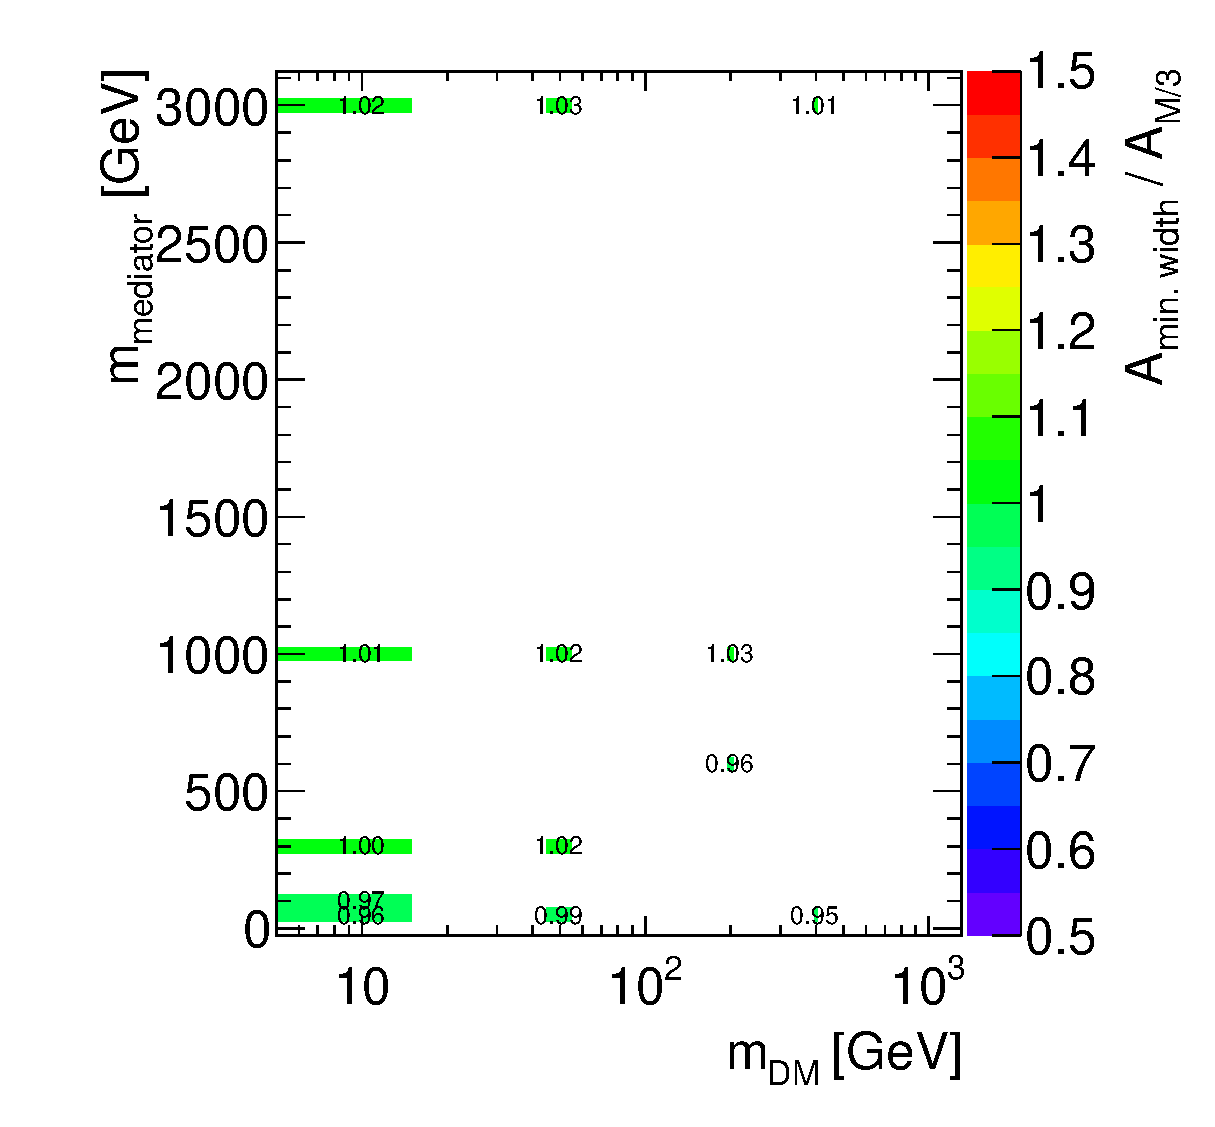
\includegraphics[width=0.7\textwidth]{figures/EW/acceptance_minwidth_vs_mo3_gamma}
%%     \caption{Analysis acceptance for the photon+\MET analysis when varying the mediator width, in the
%%     case of a vector mediator exchanged in the $s-$channel}%This plot will come from Marie-Helene
%%     \label{fig:DMV_EW_gamma_acceptance}
%% \end{figure}

Examples of relevant kinematic distributions for selected benchmark points are
shown in Fig.~\ref{fig:DMV_EW_kinematics_SVMed}. 
leading-order cross-sections for the chosen 
benchmark points are shown in Appendix~\ref{app:EWSpecificModels_Appendix}.

\begin{figure}[h!]
\centering  
\subfloat[Missing transverse momentum distribution for the photon+\MET final state, for 
different mediator mass choices, for \mdm=10~\gev.\label{fig:DMV_EW_gamma_MET_SVMed}]{%
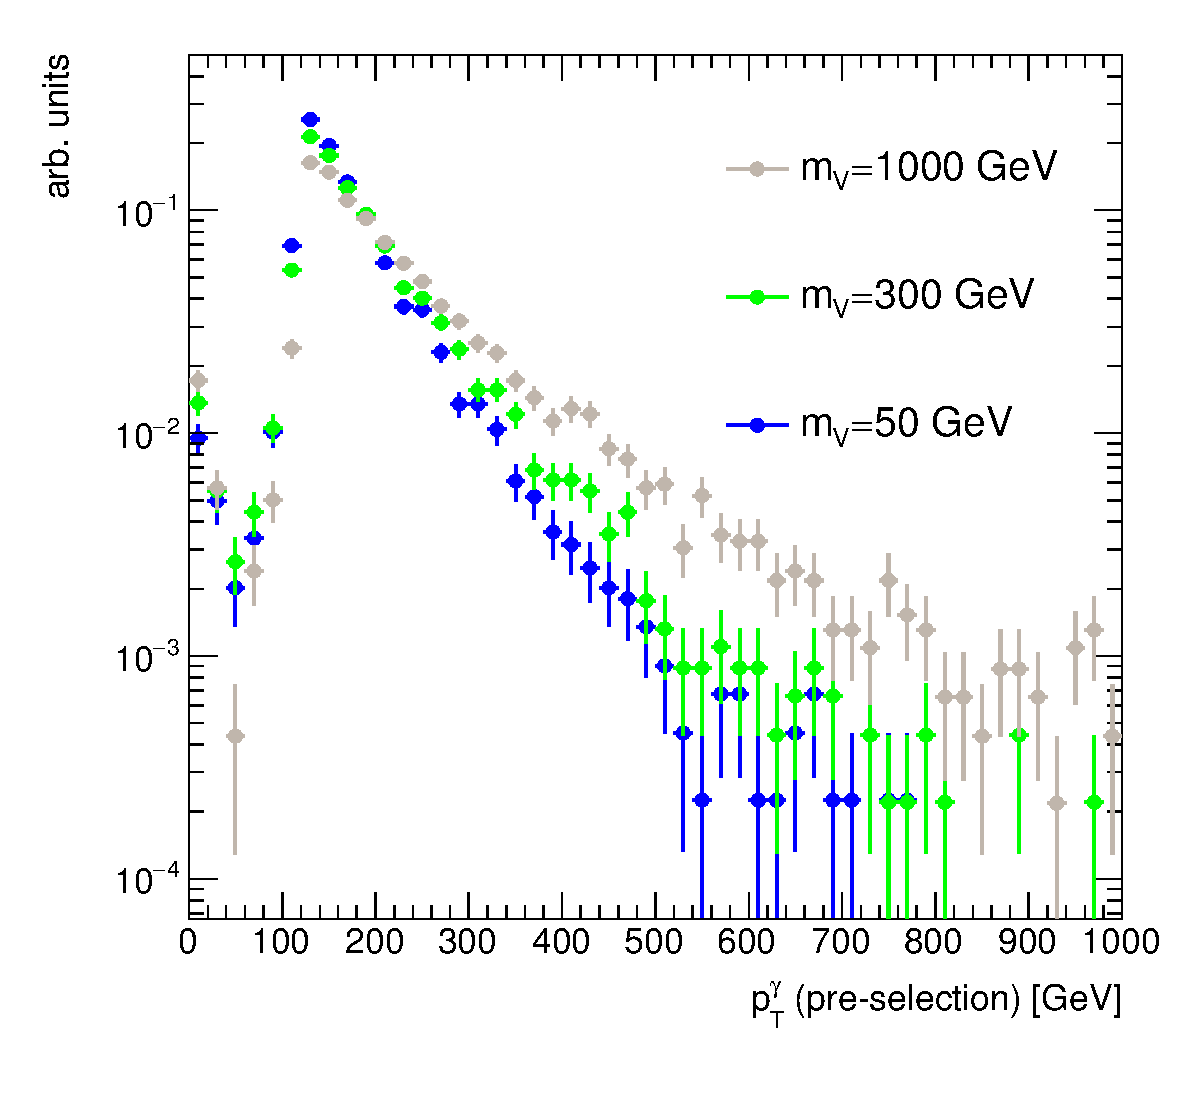
\includegraphics[width=0.45\textwidth]{figures/EW/ptGamma_filter120GeV_dmV_dm10GeV}
}%TODO: add this + equivalent plot of \MET to appendix
\hfill
\subfloat[Leading photon transverse momentum distribution for the photon+\MET final state, 
for different DM mass choices, with \mMed=1~\tev.\label{fig:DMV_EW_gamma_pT_SVMed}]{%
		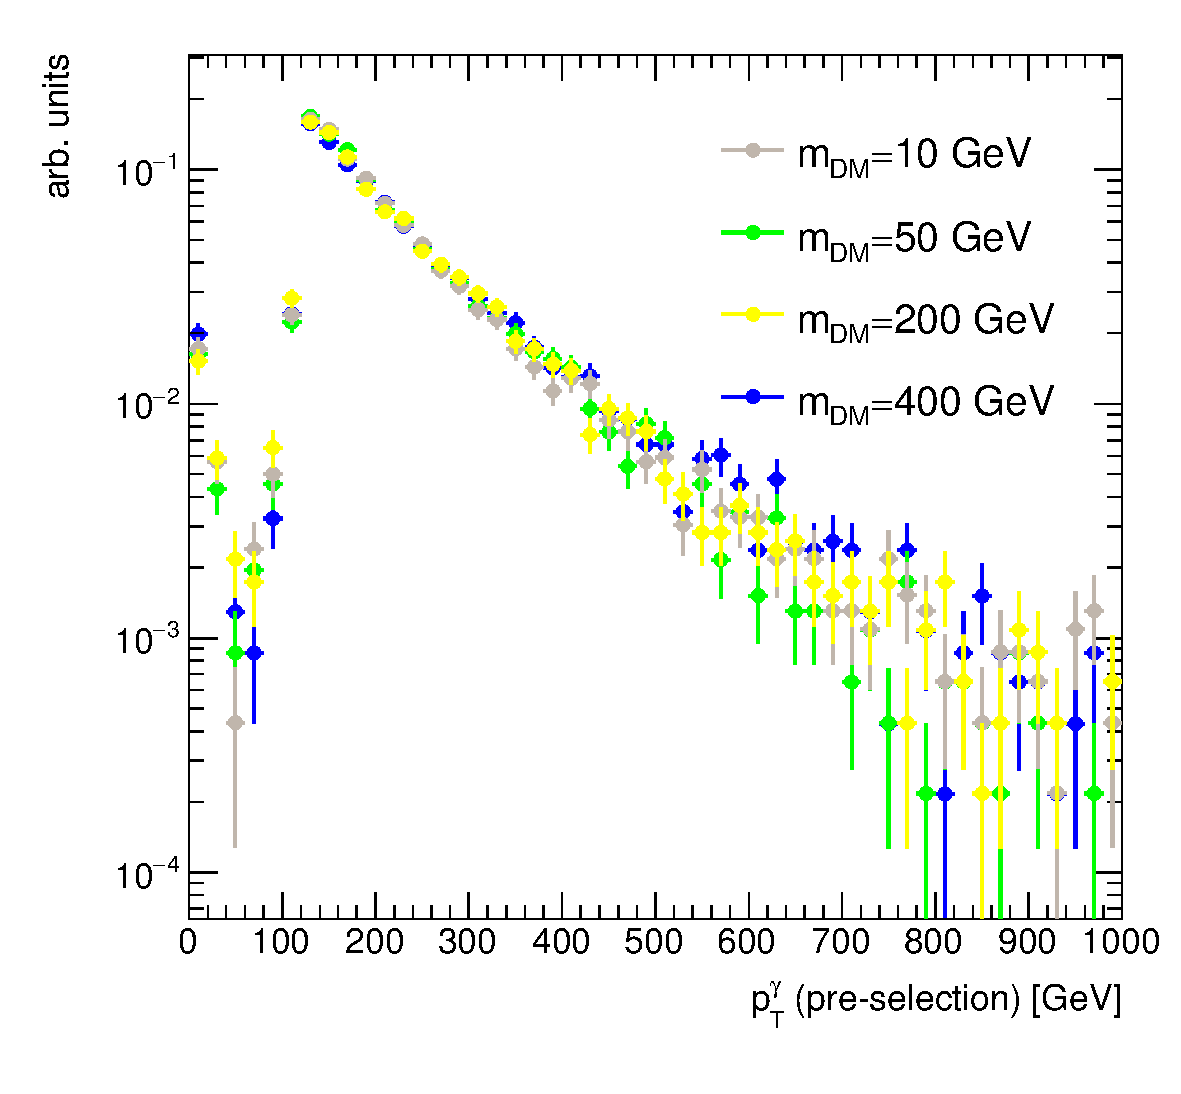
\includegraphics[width=0.45\textwidth]{figures/EW/ptGamma_filter120GeV_dmV_mV1000GeV}
}%TODO: add equivalent plot of \MET to appendix
\hfill
\subfloat[Missing transverse momentum distribution for the leptonic Z+\MET final state, 
for different mediator mass choices, for \mdm=15~\gev\label{fig:DMV_EW_Z_MET_SVMed}]{%
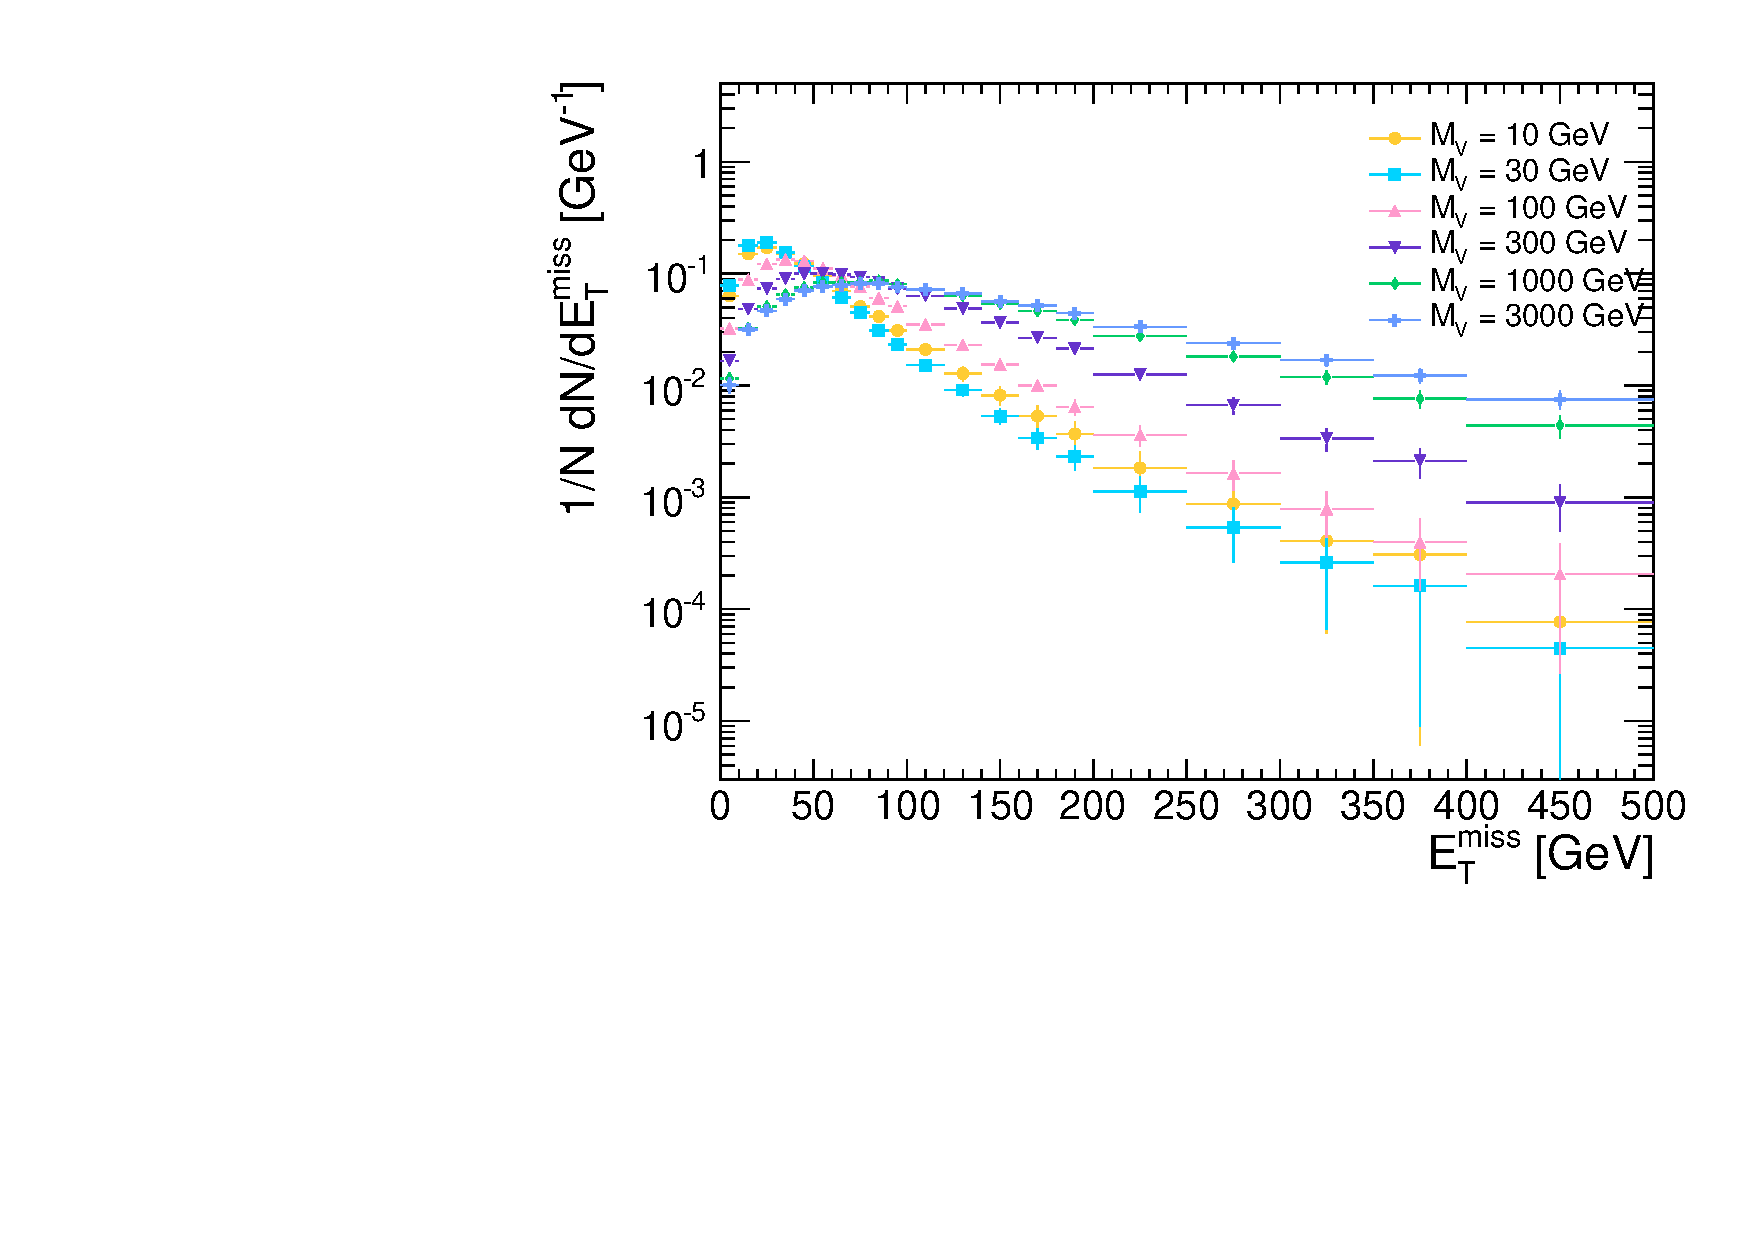
\includegraphics[width=0.45\textwidth]{figures/EW/pt_vv_Mx15}
}    
\hfill
\subfloat[Missing transverse momentum distribution for the hadronic W+\MET final state.\label{fig:DMV_EW_Whad_MET_SVMed}]{%
	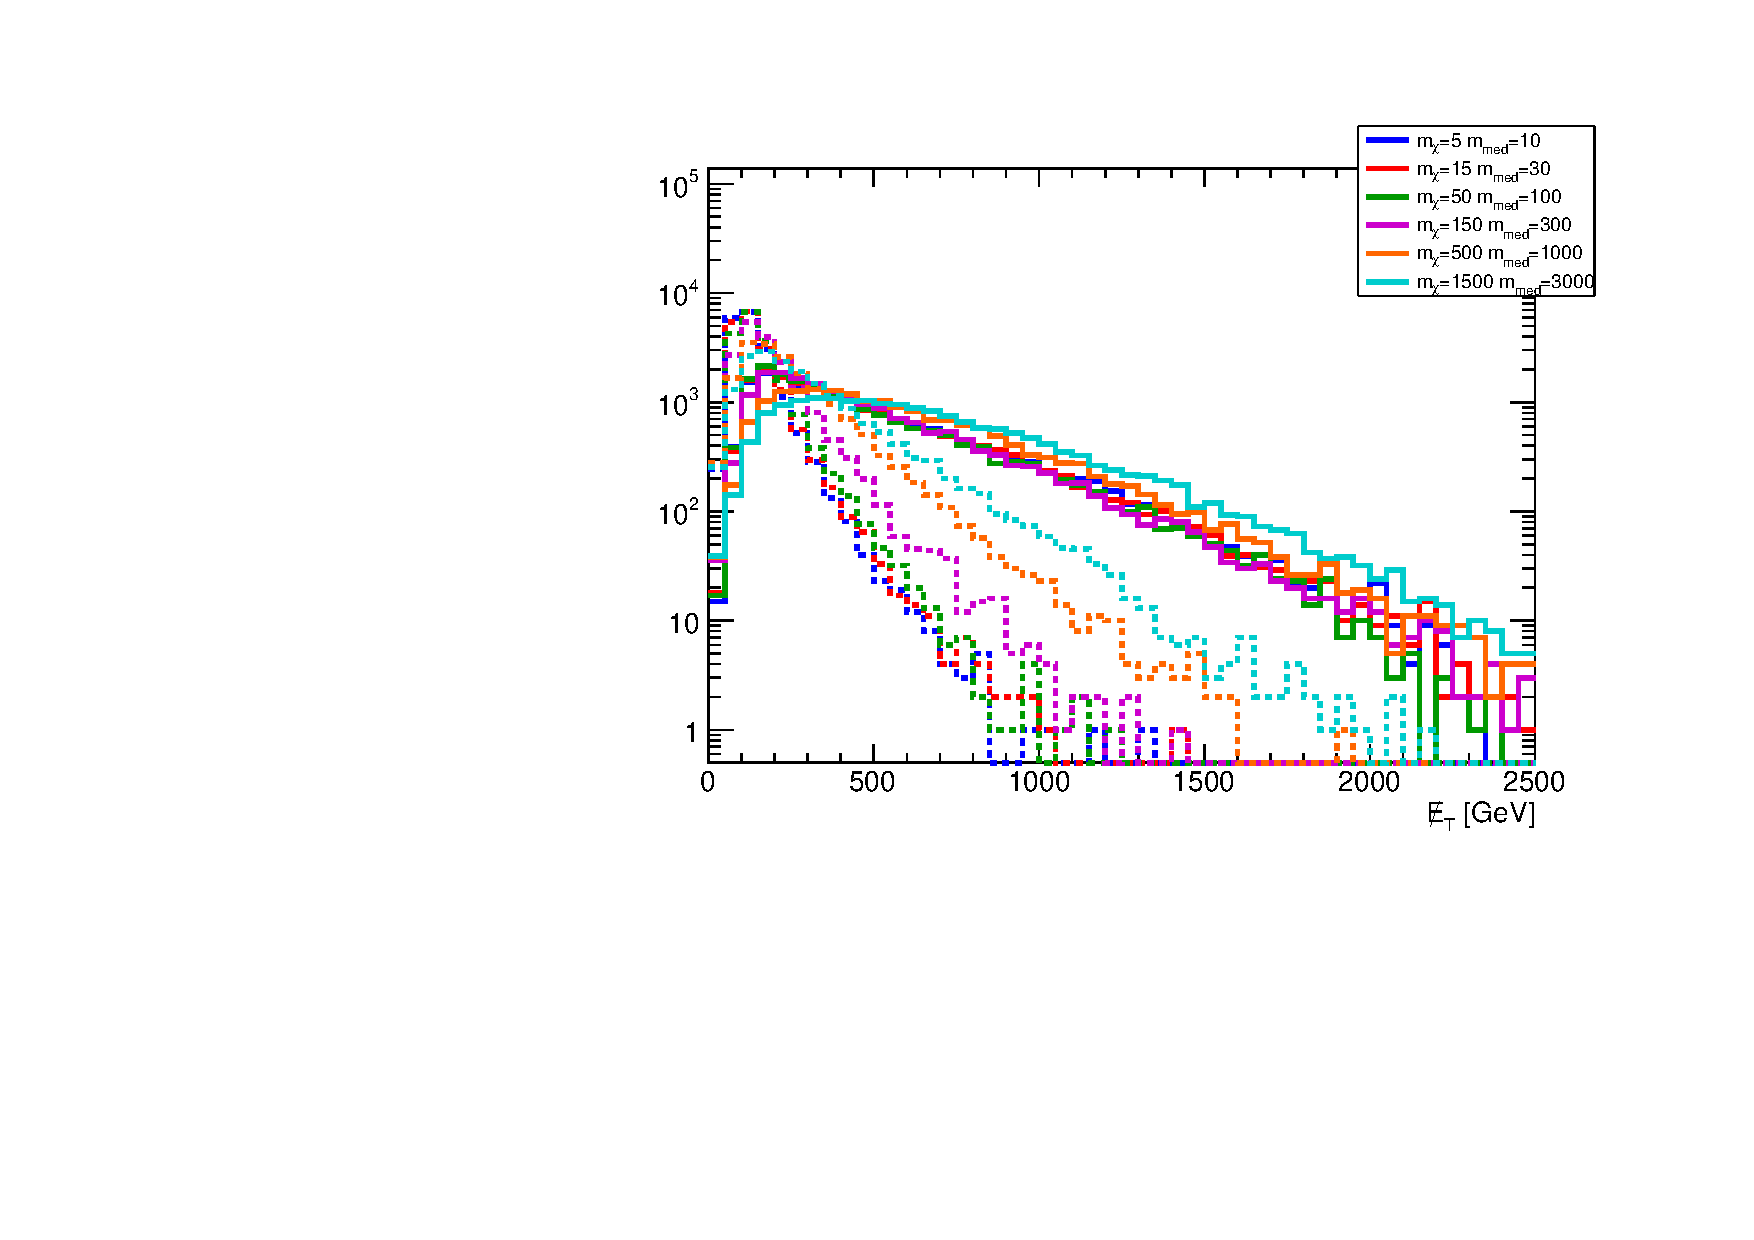
\includegraphics[width=0.5\textwidth]{figures/EW/monoWhad_Destructive/metPt}
}    
\caption{Kinematic distributions relevant for searches with W, Z and photons in the final state, 
for the simplified model
       with a vector mediator exchanged in the $s-$channel.}
\label{fig:DMV_EW_kinematics_SVMed}
\end{figure}

In addition, for the vector models considered, initial and final state radiation of a $Z'$ can occur which can appear as a narrow jet if it decays hadronically and may not be distinguishable from a QCD jet, thus accounting for some fraction of the monojet signal. The ISR and FSR of $Z'$ becomes more important at large values of the couplings~\cite{Bai:2015nfa}. 
%%%%%%%%%%%%%%%
%%%%%%%%%%%%%%%
%%%%%%%%%%%%%%%
% S/P SIMPLIFIED MODELS%
%%%%%%%%%%%%%%%
%%%%%%%%%%%%%%%
%%%%%%%%%%%%%%%

\section{Scalar and pseudoscalar mediator, \schannel exchange}
\label{sec:monojet_scalar}

\begin{figure}
\centering
\unitlength=0.005\linewidth
	\subfloat[\label{subfig:appendixmodelSmonojetTopTriangle}]	{
	\begin{feynmandiagram}[appendixmodelSmonojetTopTriangle]
		\fmfleft{i1,i2}
		\fmfright{o1,o2}
		\fmftop{isr}
		\fmfbottom{pisr}
		\fmfpolyn{empty}{v}{3}
		\fmf{fermion}{i2,v6}
		\fmf{phantom}{i1,pv1,v1}
		\fmf{gluon,tension=0}{i1,v1}
		\fmf{gluon}{v6,v3}
		\fmf{dashes,label={\LARGE $S,,P$}}{v2,v5}
		\fmf{fermion,tension=1.2}{o2,v5,o1}
		\fmfdot{v1,v6,v2,v3,v5}
		\fmffreeze
		\fmf{phantom}{pv1,pisr}
		\fmf{fermion}{v6,isr}
		\fmflabel{\LARGE ${g}$}{i1}
		\fmflabel{\LARGE ${q}$}{i2}
		\fmflabel{\LARGE ${q}$}{isr}
		\fmflabel{\LARGE $\bar\chi$}{o1}
		\fmflabel{\LARGE $\chi$}{o2}
	\end{feynmandiagram}
}
	\subfloat[\label{subfig:appendixmodelSmonojetTopBox}]	{
	\begin{feynmandiagram}[appendixmodelSmonojetTopBox]
		\fmfleft{i1,i2}
		\fmfright{o1,o2,hisr,isr}
		\fmfpolyn{empty}{v}{4}
		\fmf{gluon}{i2,v4}
		\fmf{gluon}{i1,v1}
		\fmf{dashes,label={\LARGE $S,,P$}}{v2,vwimp}
		\fmflabel{\LARGE ${g}$}{i1}
		\fmflabel{\LARGE ${g}$}{i2}
		\fmflabel{\LARGE ${g}$}{isr}
		\fmflabel{\LARGE $\bar\chi$}{o1}
		\fmflabel{\LARGE $\chi$}{o2}
		\fmf{fermion}{o2,vwimp,o1}
		\fmfdot{v1,v2,v3,v4,vwimp}
		\fmf{gluon}{v3,isr}
	\end{feynmandiagram}
}
\setfloatalignment{t}
\vspace{0.5\baselineskip}
	\caption
	{
		One-loop diagrams of processes exchanging a scalar ($S$) or pseudoscalar ($P$) mediator, leading to a mono-jet signature. 
	}
	\label{fig:feyn_prod_S}
\end{figure}

In this section, we consider a parallel situation to the vector and axial-vector mediators in the previous sections: a real scalar or a pseudoscalar where the associated scalar is decoupled at higher energies\sidenote{This assumption does not hold in a UV-complete model where the two components of the complex scalar mediator would be approximately degenerate.  The complex scalar case could be studied separately in the case of heavy flavor final states given the sufficiently different kinematics.}. This section is largely based on Refs.~\cite{Buckley:2014fba,Harris:2014hga} which contain a thorough discussion of these models. 

Assuming MFV, \spinzero resonances behave in a similar fashion as the SM Higgs boson. Relative to the vector and axial-vector models discussed above, the scalar models are distinguished by the special consequences of the MFV assumption: the very narrow width of the mediator and its extreme sensitivity to which decays are kinematically available, and the loop-induced coupling to gluons. The interaction Lagrangians are

\begin{fullwidth}
  \begin{eqnarray} {\cal L}_{\phi} & = &
    % {\cal L}_{\rm SM}+i\bar{\chiDM} \slashed{\partial} \chiDM + \mDM \bar{\chiDM}\chiDM + \left| \partial_\mu \phi \right|^2+\frac{1}{2}m_\phi^2 \phi^2 + \nonumber \\
    % & &
          \gdm \phi \bar{\chiDM}\chiDM+ \frac{\phi}{\sqrt{2}} \sum_i \left(g_u y_i^u \bar{u}_i u_i+g_d y_i^d \bar{d}_i d_i+g_\ell y_i^\ell \bar{\ell}_i \ell_i\right)\, , \label{eq:scalarlag} \\
    {\cal L}_{a} & = &
    % {\cal L}_{\rm SM}+i\bar{\chiDM} \slashed{\partial} \chiDM + \mDM \bar{\chiDM}\chiDM + \left| \partial_\mu a \right|^2+\frac{1}{2}m_a^2 a^2 + \nonumber \\
    % & &
          i\gdm a \bar{\chiDM}\gamma_5\chiDM+ \frac{i a}{\sqrt{2}}\sum_i  \left(g_u y_i^u \bar{u}_i \gamma_5 u_i+g_d y_i^d \bar{d}_i \gamma_5 d_i+ \right. \nonumber \\
                                   & & \left. g_\ell y_i^\ell   \bar{\ell}_i \gamma_5 \ell_i\right) \,. \label{eq:pseudoscalarlag}
  \end{eqnarray}
\end{fullwidth}
where $\phi$ and $a$ are respectively the scalar and pseudoscalar mediators, and the Yukawa couplings $y_i^f$ are normalized to the Higgs vev as $y_i^f = \sqrt{2}m_i^f/v$.

The couplings to fermions are proportional to the SM Higgs couplings, yet one is still allowed to adjust an overall strength of the coupling to charged leptons and the relative couplings of $u$- and $d$-type quarks. As in the preceding sections, for the sake of simplicity and straightforward comparison, we reduce the couplings to the SM fermions to a single universal parameter $\gq \equiv g_u = g_d = g_\ell$. Unlike the vector and axial-vector models, the scalar mediators are allowed to couple to leptons.\sidenote{This contribution plays no role for most of the parameter space considered. The choice to allow lepton couplings follows Refs.~\cite{Buckley:2014fba,Harris:2014hga}.}


The relative discovery and exclusion power of each search can be compared in this framework.
However, we again emphasize the importance of searching the
full set of allowed channels in case violations of these simplifying assumptions
lead to significant modifications of the decay rates that
unexpectedly favor different
channels than the mix obtained under our assumptions. The coupling $\gdm$ parameterizes the entire dependence on the structure between the mediator and the dark sector.

%The most general Lagrangians including new scalars or pseudoscalars will have a potential containing interactions with the SM Higgs field $h$. 
 %If there is no indication otherwise the easiest assumptions is always the most scientific to chose (also listening to some phenomenologists this seems not always to be the case ;-) )  

Given these simplifications, the minimal set of parameters under consideration is
 \bea
  \left\{ \mDM,~ m_{\phi/a} = \mMed,~ \gdm,~ \gq \right\} \,.
 \eea
Fig.~\ref{fig:feyn_prod_S} shows the one-loop diagrams producing a jet+X signature. 
The full calculation of the top loop is available at LO for DM pair production in association with one parton. 


%The simplest choice of couplings, known as Minimal Simplified Dark Matter model (MSDM) \textbf{[TODO: add references]}, is $g_u = g_d = g_\ell$, which is realized in singlet scalar extensions of the SM. 

% Despite our simplifying assumption, one should keep the more general possibility in mind, as even simple extensions of the mediating sector can result in $g_u \neq g_d \neq g_\ell$. A well-known realization of this would be the coupling of the pseudoscalar to up-type quarks (proportional to $m_u \cot\beta$) and down-type quarks and charged leptons (proportional to $m_{d/\ell}\tan\beta$) in two-Higgs doublet extensions of the SM. Here $\tan \beta$ denoting the ratio of vacuum expectation values of the two Higgs doublets. %The case $g_u \neq  g_d \neq g_\ell$ requires additional scalars with potentially large masses. 
% This possibility of non-equal couplings motivates searches in complementary channels which probe couplings to different flavors of quarks and leptons.

%Extending the SM Higgs sector to a two Higgs doublet model implies more complex couplings such as  $g_u = \cot \beta$ and $g_d = g_e = \tan \beta$ where $\tan \beta$ denotes the ratio of vacuum expectation values of the two Higgs doublets.  The case $g_u \neq  g_d \neq g_\ell$ requires more additional scalars with potentially large masses, and it is not covered here: for simplicity, we assume universal SM-mediator couplings $g_v = g_u = g_d = g_\ell$ in the remainder of this work. 


%The model assumes Dirac Dark Matter particles and is based on the minimal flavor violation (MFV), which motivates Higgs-like Yukawa couplings of the mediator to the Standard Model quarks. No other couplings, such as to leptons, are allowed in this model.
%The following two cases are considered:\\
%(a) scalar couplings to DM and SM,\\
%(b) pseudo-scalar couplings to DM and SM\\
%\noindent with the corresponding Lagrangians written as:
%\begin{align}
%\label{eq:SP} 
%\mathcal{L}_{\mathrm{scalar}} &= \gq \sum \frac{m_q}{v} (\bar{q}q) S + \gDM (\bar{\chiDM}\chiDM) S \\
%\mathcal{L}_{\mathrm{pseudo-scalar}} &= \gq \sum \frac{m_q}{v} (\bar{q}\gamma^5q) P + \gDM (\bar{\chiDM}\gamma^5\chiDM) P \\
%\end{align}
%where $v=246$~\gev denotes the Higgs vacuum expectation value.

The minimal mediator width is given by %Eq.\,\ref{eq:monojet_min},
\begin{fullwidth}
  \begin{equation} \label{eq:width}
    \begin{split}
      \Gamma_{\phi,a} = & \sum_f N_c \frac{y_f^2 \gq^2 m_{\phi,a}}{16
        \pi} \left(1-\frac{4 m_f^2}{m_{\phi,a}^2}\right)^{x/2}
      + \frac{\gdm^2 m_{\phi,a}}{8 \pi} \left(1-\frac{4 \mDM^2}{m_{\phi,a}^2}\right)^{x/2}\\
      & + \frac{\alpha_s^2 y_t^2 \gq^2 m_{\phi,a}^3}{32 \pi^3 v^2}
      \left| f_{\phi,a}\left(\tfrac{4m_t^2}{m_{\phi,a}^2}
        \right)\right|^2
    \end{split}
  \end{equation}
\end{fullwidth}
where $x=3$ for scalars and $x=1$ for pseudoscalars. The loop integrals are
\begin{fullwidth}
  \bea \label{eq:fphifa}
  f_\phi (\tau) &=& \tau \left [ 1+ (1-\tau) \arctan^2 \left ( \frac{1}{\sqrt{\tau-1}} \right ) \right ]  \,, \\
  f_a (\tau) &=& \tau \arctan^2 \left ( \frac{1}{\sqrt{\tau-1}}
  \right) \, 
  \eea
\end{fullwidth}
for $\tau < 1$, where $\tau = 4 m_{t}^2/m_{\phi,a}^2$, and, for $\tau > 1$, 
\begin{fullwidth}
  \bea \label{eq:fphifb}
  f_\phi (\tau) &=& \tau \left [ 1+ (1-\tau)\left(-\frac{1}{4}\left(\log\frac{1+\sqrt{1-\tau}}{1-\sqrt{1-\tau}}+i\pi\right)^2\right) \right ]  \,\,,\\
  f_a (\tau) &=& \tau
  \left(-\frac{1}{4}\left(\log\frac{1+\sqrt{1-\tau}}{1-\sqrt{1-\tau}}+i\pi\right)^2\right).
  \eea
\end{fullwidth}


% If this is in the DM@LHC write-up, it is unnecessary here.
% The first term in the width corresponds to the decay into SM fermions, and the sum runs over all kinematically available fermions, $N_c = 3$ for quarks. The second term is the decay into DM, assuming that is kinematically allowed. The factor of two between the decay into SM  fermions and into DM  is a result of our choice of normalization of the Yukawa couplings due to spin dependencies. The last term corresponds to decay into gluons.  Since we have assumed that $\gq = g_u = g_d = g_\ell$, we have included in the partial decay widths $\Gamma (\phi/a \to gg)$ only the contributions stemming from top loops, which provide the by far largest corrections given that $y_t \gg y_b$~etc. At the loop level the mediators can decay not only to gluons but also to pairs of photons and other final states if kinematical accessible. However the decay rates $\Gamma (\phi/a \to gg)$ are always larger than the other loop-induced partial widths, and in consequence the total decay widths $\Gamma_{\phi/a}$ are well approximated by the corresponding sum of the individual partial decay widths involving DM, fermion or gluon pairs. It should be noted that if  $m_{\phi/a} > 2m_t$ the total widths of $\phi/a$ will typically be dominated by the partial widths to top quarks.


%\begin{equation}
%\Gamma_{\rm{min}}^{S/P}=\Gamma_{\bar{\chiDM}\chiDM}^{S/P} + \sum_{q}\Gamma_{\bar{q}q}^{S/P} + \Gamma_{gg}^{S/P},
%\end{equation}
%with the following LO expressions for the partial widths:
%\begin{align}
%\Gamma_{\bar{\chiDM}\chiDM}^{\rm{S}}&=\frac{\gDM^2 \mMed}{8\pi}\beta_{DM}^{3/2} \theta(\mMed-2\mDM)\\
%\Gamma_{\bar{q}q}^{\rm{S}}&= \frac{3 \gq^2 \mMed}{8\pi}\frac{m_q^2}{v^2}\beta_q^{3/2} \theta(\mMed-2m_q)\\
%\Gamma_{gg}^{\rm{S}}&= \frac{\gq^2 \alpha_s^2}{2\pi^3 v^2 \mMed} \left| \sum_q m_q^2 F_{\rm{S}} \left( \frac{4m_q^2}{\mMed^2} \right) \right|^2\\
%\Gamma_{\bar{\chiDM}\chiDM}^{\rm{P}}&=\frac{\gDM^2 \mMed}{8\pi} \beta_{DM}\theta(\mMed-2\mDM)\\
%\Gamma_{\bar{q}q}^{\rm{P}}&= \frac{3 \gq^2 \mMed}{8\pi}\frac{m_q^2}{v^2}\beta_{q}\theta(\mMed-2m_q)\\
%\Gamma_{gg}^{\rm{P}}&= \frac{\gq^2 \alpha_s^2}{2\pi^3 v^2 \mMed} \left| \sum_q m_q^2 F_{\rm{P}} \left( \frac{4m_q^2}{\mMed^2} \right) \right|^2\;,
%\label{eq:GammaS}
%\end{align}
%with the form factors defined as
%\begin{align}
%F_{\rm{S}}(x)&= 1+(1-x)\arctan^2\left(\frac{1}{\sqrt{x-1}}\right)\\
%F_{\rm{P}}(x)&= \arctan^2\left(\frac{1}{\sqrt{x-1}}\right)\;.
%\end{align}

%%Start Matt Buckley's edits 
%\begin{equation} \label{eq:width}
%\begin{split}
%\Gamma_{\phi,a}  = & \sum_f N_c \frac{y_f^2 \gq^2 m_{\phi,a}}{16 \pi} \left(1-\frac{4 m_f^2}{m_{\phi,a}^2}\right)^{x/2}
%+ \frac{\gdm^2 m_{\phi,a}}{8 \pi} \left(1-\frac{4 \mDM^2}{m_{\phi,a}^2}\right)^{x/2}\\
%& + \frac{\alpha_s^2 y_t^2 \gq^2 m_{\phi,a}^3}{32 \pi^3 v^2} \left| f_{\phi,a}\left(\tfrac{4m_t^2}{m_{\phi,a}^2} \right)\right|^2
%\end{split}
%\end{equation}
%
%where $x=3$ for scalars and $x=1$ for pseudoscalars, and the loop integrals are
%
%\bea \label{eq:fphifa}
%f_\phi (\tau) = \tau \left [ 1+ (1-\tau) \arctan^2 \left ( \frac{1}{\sqrt{\tau-1}} \right ) \right ]  \,, \qquad 
%f_a (\tau) =  \tau \arctan^2 \left ( \frac{1}{\sqrt{\tau-1}} \right ) \,. 
%\eea
%
%The first term in each width corresponds to the decay into SM fermions (the sum runs over all kinematically available fermions, $N_c = 3$ for quarks and $N_c = 1$ for leptons). The second term is the decay into DM (assuming that this decay is kinematically allowed). The factor of two between the decay into SM  fermions and into DM  is a result of our choice of normalization of the Higgs vacuum expectation value and the Yukawa couplings.
%

%%BP: Is this the best way to express that? I'd add:... due to spin dependencies. 
%%MB: yes. I don't think it's a spin thing, it's just that we've defined v = 246, so the SM fermions get a $1/\sqrt{2}^2$ that DM doesn't.

%The last two terms correspond to decay into gluons.  Since we have assumed that $\gq = g_u = g_d = g_\ell$, we have included in the partial decay widths $\Gamma (\phi/a \to gg)$ only the contributions stemming from top loops, which provide the by far largest corrections given that $y_t \gg y_b$~etc. At the loop level the mediators can decay not only to gluons but also to pairs of photons and other final states if kinematical accessible. However the decay rates $\Gamma (\phi/a \to gg)$ are always larger than the other loop-induced partial widths, and in consequence the total decay widths $\Gamma_{\phi/a}$ are well approximated by the corresponding sum of the individual partial decay widths involving DM, fermion or gluon pairs. It should be noted that if  $m_{\phi/a} > 2m_t$ the total widths of $\phi/a$ will typically be dominated by the partial widths to top quarks.

%%%End Matt Buckley's edits

The minimal widths for scalar and pseudo-scalar mediators with $\gq=\gDM=1$ are shown in Fig.\,\ref{fig:monojet_width_S}, illustrating the effect of choosing
the SM Higgs-like Yukawa couplings for the SM fermions.
For the mediator mass above twice the top quark mass $m_t$, the minimal width receives the dominant contribution from the top quark. For lighter mediator masses, Dark Matter dominates as the couplings to lighter quarks are Yukawa suppressed.
%Note that the partial width coming from gluons through loops can be safely neglected\,\cite{Haisch:2015ioa}.


\begin{figure}
\centering
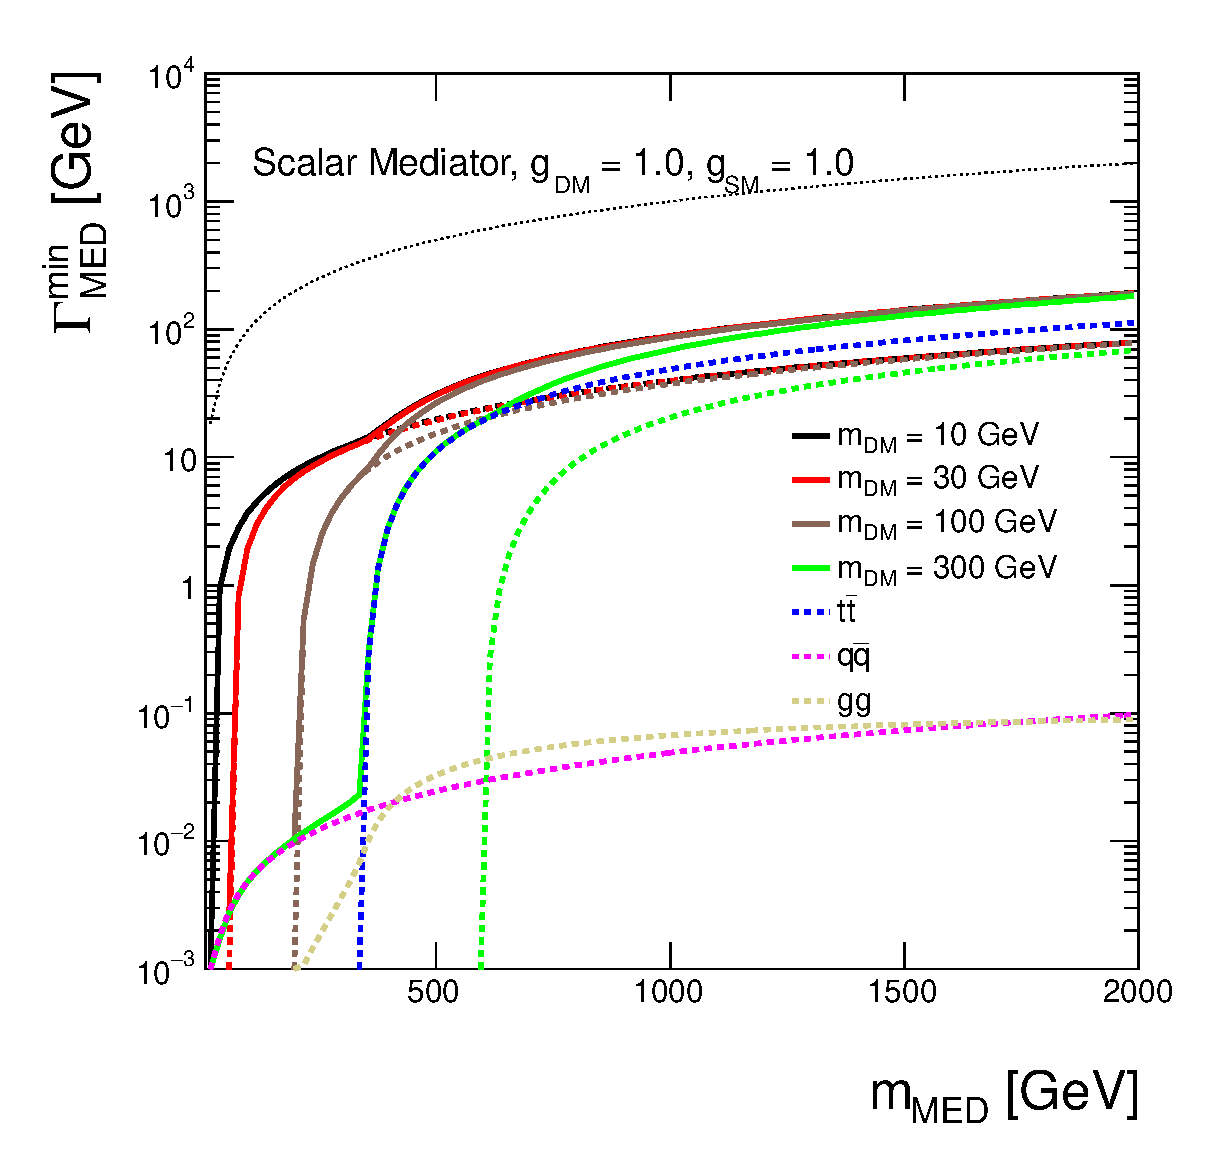
\includegraphics[width=0.95\textwidth]{figures/monojet/width_S.eps}
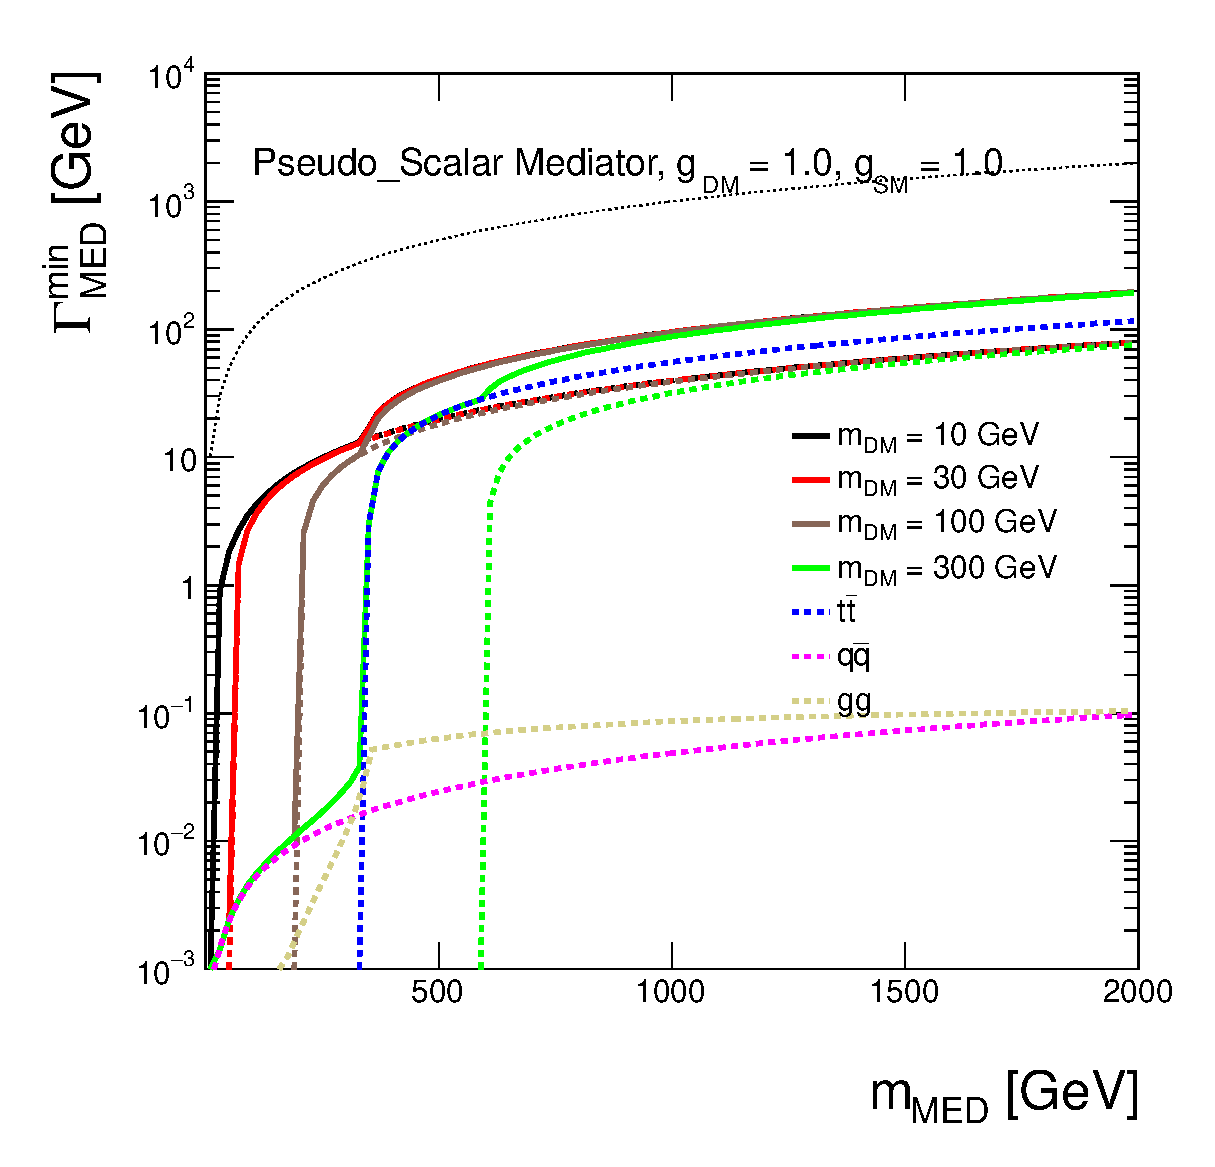
\includegraphics[width=0.95\textwidth]{figures/monojet/width_P.eps}
\caption{Minimal width as a function of mediator mass for scalar and pseudo-scalar mediator assuming couplings of 1. The total width is shown as solid lines for Dark Matter masses of \mDM=10~\gev, 30~\gev, 100~\gev and 300~\gev in black, red, brown and green, respectively. The individual contributions from Dark Matter are indicated by dotted lines with the same colors. The contribution from all quarks but top is shown as magenta dotted line and the contribution from top quarks only is illustrated by the dotted blue line. The dotted beige line shows the contribution from the coupling to gluons. The dotted black line shows the extreme case $\Gamma_{\rm{min}}=\mMed$.}
\label{fig:monojet_width_S}
\end{figure}

It can be seen in Fig.~\ref{fig:monojet_SPmodels} that the kinematics for the scalar and pseudoscalar models coincides when considering the diagrams in Fig.~\ref{fig:feyn_prod_S}. 
For this reason, we recommend to generate only one of the two models.
%, and report the cross-sections on HEPData 
%for the other one.
No preference is given between the two models as they have the
same kinematics, although it is worth noting that the pseudo-scalar model has been used for a Dark Matter interpretation of the DAMA signal 
and of the galactic center excess~\cite{Arina:2014yna}.
Like in the case of the vector and axial-vector models described in Section~\ref{sec:monojet_spin}, the differences between the cross sections for the scalar and pseudo-scalar samples with the same $\mDM$ and $\mMed$ are increasing with the Dark Matter mass for fixed mediator mass. The pseudo-scalar model gives larger cross sections. Also note the increasing differences between the minimal widths close to the $2\mDM=\mMed$ threshold.

\begin{figure*}
	\centering
	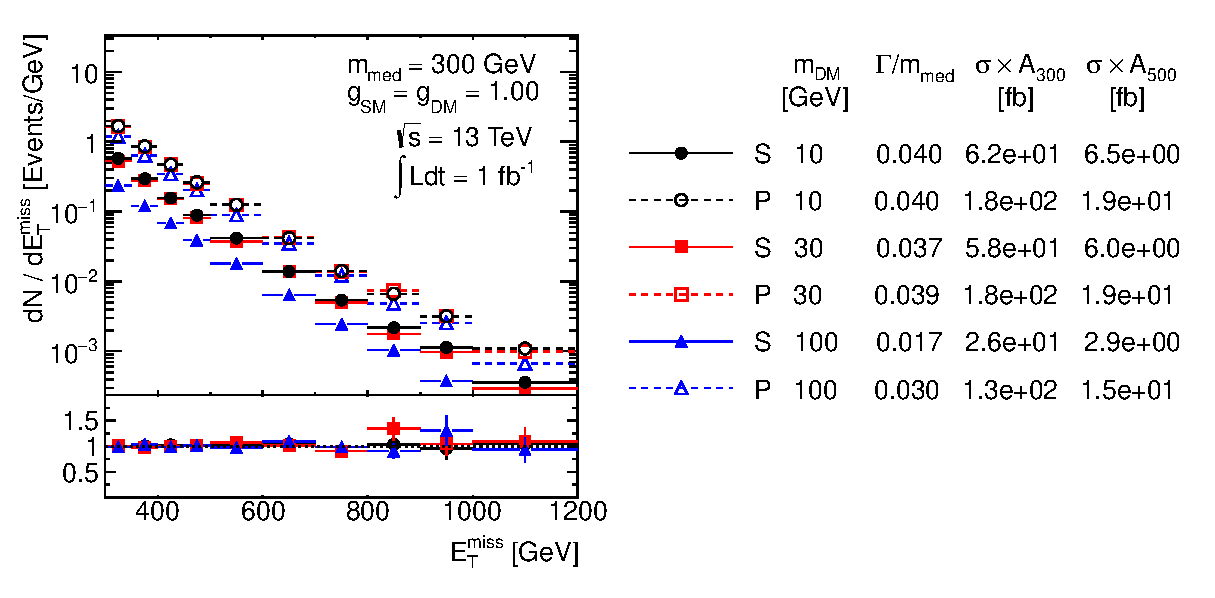
\includegraphics[width=0.95\textwidth]{figures/monojet/compareModels_SP_300.eps}
	\caption{Comparison of the $\MET$ distributions for the scalar and pseudoscalar models for different $\mMed=300\,\gev$ and different Dark Matter masses. 
	Ratios of the normalized distributions with respect to the first one are shown. $A_{300}$ and $A_{500}$ in the table denote the acceptance of the $\MET>300$~\gev and $\MET>500$~\gev cut, respectively.}
	\label{fig:monojet_SPmodels}
\end{figure*}



\subsection{Parameter scan}

Similarly as in the case of the vector and axial-vector couplings
of \spinone mediators, scans in the parameter space are performed also for the scalar and pseudo-scalar couplings of the \spinzero mediators
in order to decide on the optimized parameter grid for the presentation of Run-2 results. Figures\,\ref{fig:monojet_scan_S_g}-
%, fig:monojet_scan_S_mDM1000,fig:monojet_scan_S_mDM100, fig:monojet_scan_S_mMed10, 
\ref{fig:monojet_scan_S_mMed1000} show the scans over the couplings, Dark Matter mass and mediator mass and the same conclusions apply as in Section\,\ref{sec:monojet_V}.

%TODO does the discussion below make sense?
A scan over the mediator mass is shown in Fig.\,\ref{fig:monojet_scan_S_mMed1000} where \mMed = 300~\gev and 500~\gev are chosen to be below and above $2m_t$. The off-shell Dark Matter production regime is assumed by taking an extreme limit ($\mDM=1$~\tev) in order to study solely the effects of the couplings to quarks. 
No differences in the kinematic distributions are observed and also the cross sections remain similar in this case. No significant changes appear for mediator masses around the $2m_t$ threshold.

\begin{figure*}[!htpb]
\centering
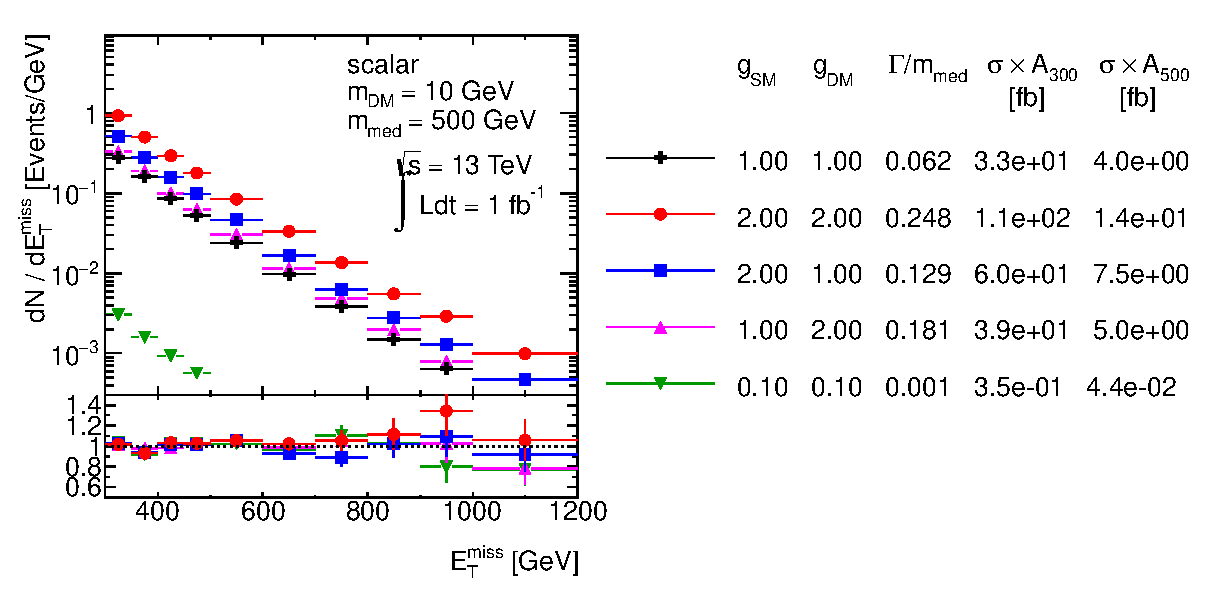
\includegraphics[width=0.95\textwidth]{figures/monojet/scan_g_S_10_500.eps}
\caption{Scan over couplings. The $\MET$ distribution is compared for the scalar mediator models using the parameters as indicated. Ratios of the normalized distributions with respect to the first one are shown. $A_{300}$ and $A_{500}$ in the table denote the acceptance of the $\MET>300$~\gev and $\MET>500$~\gev cut, respectively.}
\label{fig:monojet_scan_S_g}
\end{figure*}

\begin{figure*}[!htpb]
\centering
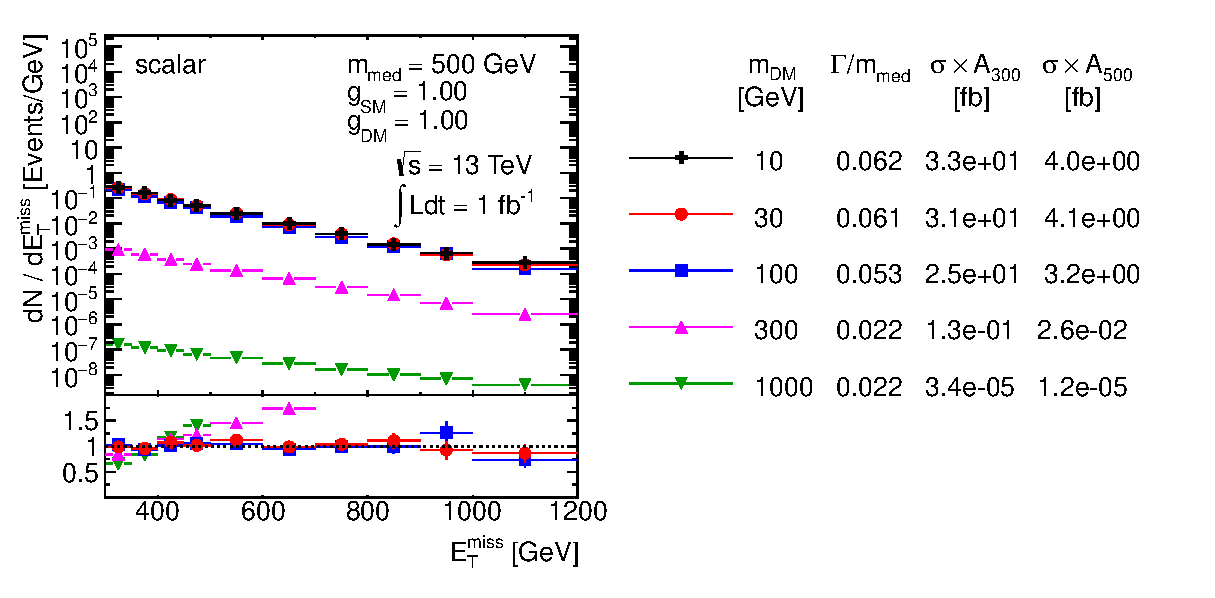
\includegraphics[width=0.95\textwidth]{figures/monojet/scan_mDM_S_500.eps}
\caption{Scan over Dark Matter mass. The $\MET$ distribution is compared for the scalar mediator models using the parameters as indicated. Ratios of the normalized distributions with respect to the first one are shown. $A_{300}$ and $A_{500}$ in the table denote the acceptance of the $\MET>300$~\gev and $\MET>500$~\gev cut, respectively.}
\label{fig:monojet_scan_S_mDM1000}
\end{figure*}

\clearpage

\begin{figure*}[!htpb]
\centering
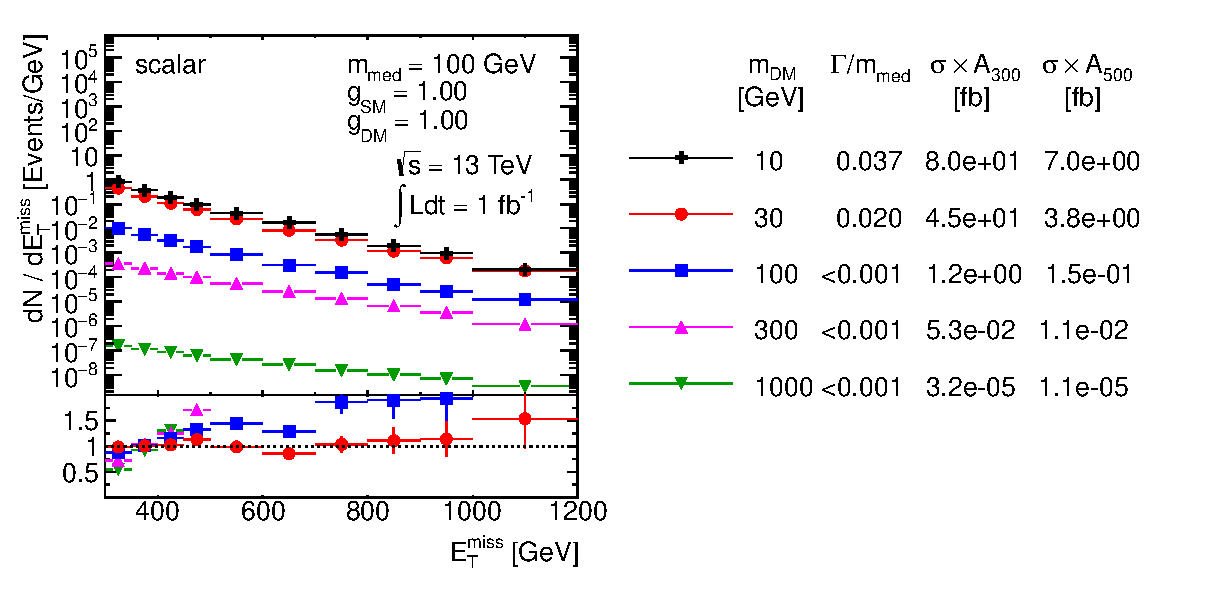
\includegraphics[width=0.95\textwidth]{figures/monojet/scan_mDM_S_100.eps}
\caption{Scan over Dark Matter mass. The $\MET$ distribution is compared for the scalar mediator models using the parameters as indicated. Ratios of the normalized distributions with respect to the first one are shown. $A_{300}$ and $A_{500}$ in the table denote the acceptance of the $\MET>300$~\gev and $\MET>500$~\gev cut, respectively.}
\label{fig:monojet_scan_S_mDM100}
\end{figure*}

\begin{figure*}[!htpb]
\centering
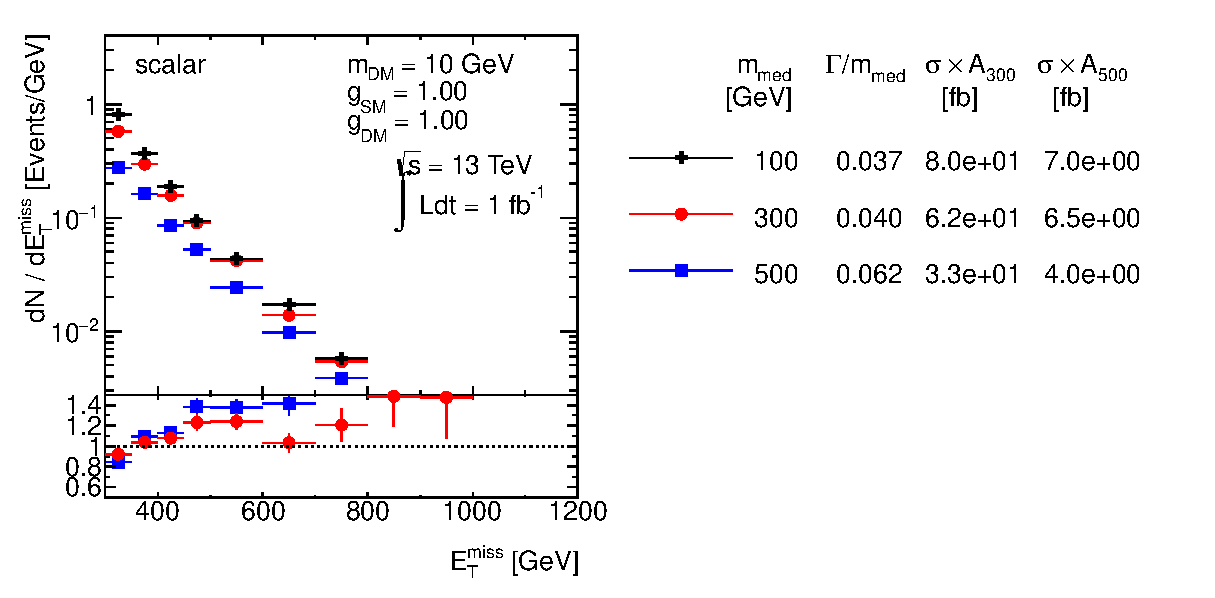
\includegraphics[width=0.95\textwidth]{figures/monojet/scan_mMed_S_10.eps}
\caption{Scan over mediator mass. The $\MET$ distribution is compared for the scalar mediator models using the parameters as indicated. Ratios of the normalized distributions with respect to the first one are shown. $A_{300}$ and $A_{500}$ in the table denote the acceptance of the $\MET>300$~\gev and $\MET>500$~\gev cut, respectively.}
\label{fig:monojet_scan_S_mMed10}
\end{figure*}

\clearpage 

\begin{figure*}[!htpb]
\centering
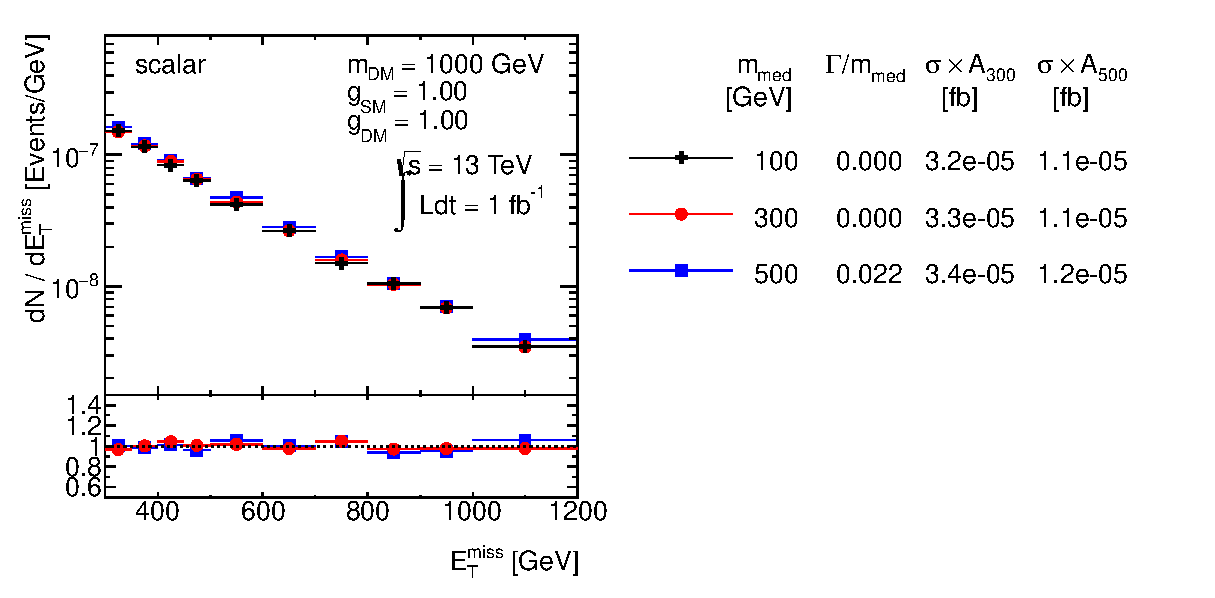
\includegraphics[width=0.95\textwidth]{figures/monojet/scan_mMed_S_1000.eps}
\caption{Scan over mediator mass. The $\MET$ distribution is compared for the scalar mediator models using the parameters as indicated. Ratios of the normalized distributions with respect to the first one are shown. $A_{300}$ and $A_{500}$ in the table denote the acceptance of the $\MET>300$~\gev and $\MET>500$~\gev cut, respectively.}
\label{fig:monojet_scan_S_mMed1000}
\end{figure*}


The optimized parameter grid in the $\mMed$--$\mDM$ plane for scalar and pseudo-scalar mediators is motivated by similar arguments as in the previous section. Therefore, a similar pattern is followed here, taking again $\gq=0.25$ and $\gDM=1$. Only the sensitivity to the highest mediator masses has to be re-evaluated.
The generator level cross section times the acceptance at $\MET>500$~\gev for the model with couplings $\gq=\gDM=1$, light Dark Matter of \mDM=10~\gev and
a \mMed=500~\gev scalar mediator is at the order of 10\,fb, i.e. just at the edge of the early Run-2 sensitivity. Increasing the mediator mass to 1~\tev pushes the product $\sigma\times A$ down to approximately 0.1\,fb, below the LHC sensitivity. Therefore, we choose to remove the 2~\tev mediator mass from the grid and present the final grid with 33
%26 
mass points only, as shown in Tab.\,\ref{tab:mDMmMedScan_SP}.
One point at very high mediator mass (10~\tev) is added for each of the DM masses scanned, to aid the reinterpretation of results in terms of contact interaction operators (EFTs). 

\begin{table}[!h]
\centering
\begin{tabular}{| l |r r r r r r r r r|}
\hline
\multicolumn{1}{|c|}{\mDM (\gev)} & \multicolumn{9}{c|}{\mmed (\gev)} \\
\hline
 1             &         10  & 20 & 50 & 100 & 200 & 300 & 500 &         1000  &         10000  \\
 10   	       &         10  & 15 & 50 & 100 &     &     &     &               &         10000  \\
 50            &         10  &    & 50 &  95 & 200 & 300 &     &               &         10000  \\
 150           &         10  &    &    &     & 200 & 295 & 500 &         1000  &         10000  \\
 500           &         10  &    &    &     &     &     & 500 &          995  &         10000  \\
 1000          &         10  &    &    &     &     &     &     &         1000  &         10000  \\
\hline
\end{tabular}

\caption{Simplified model benchmarks for \schannel simplified models (\spinzero mediators 
decaying to Dirac DM fermions in the scalar and pseudoscalar case, taking the minimum width for \gq = 0.25 and \gDM = 1)}.
% Points in \textbf{bold} are only generated for the vector/axial vector cases, while points in 
% \textit{italics} are generated for the monojet analysis 
% but not for the search including heavy quarks. This table corresponds to 29 points for monojet vector/axial vector models,
% 26 points for monojet scalar/pseudoscalar models and 24 points for $t \bar{t}$+\MET scalar/pseudoscalar models.}

\label{tab:mDMmMedScan_SP}
% \end{sidewaystable}
\end{table}

% \begin{figure}
% \centering
% 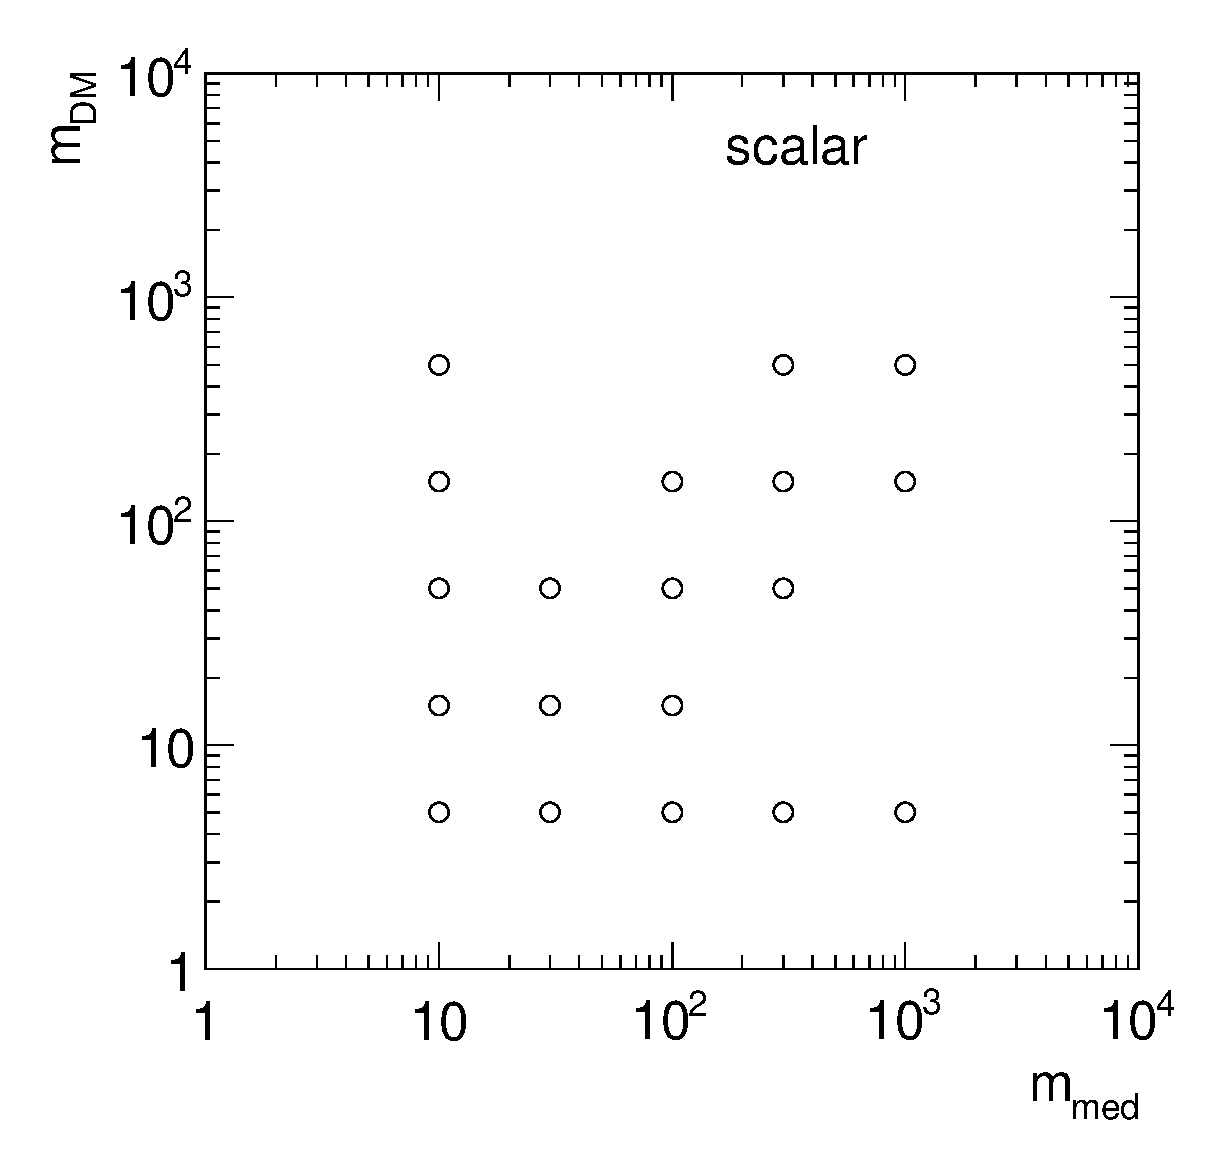
\includegraphics[width=0.95\textwidth]{figures/monojet/grid_S.eps}
% 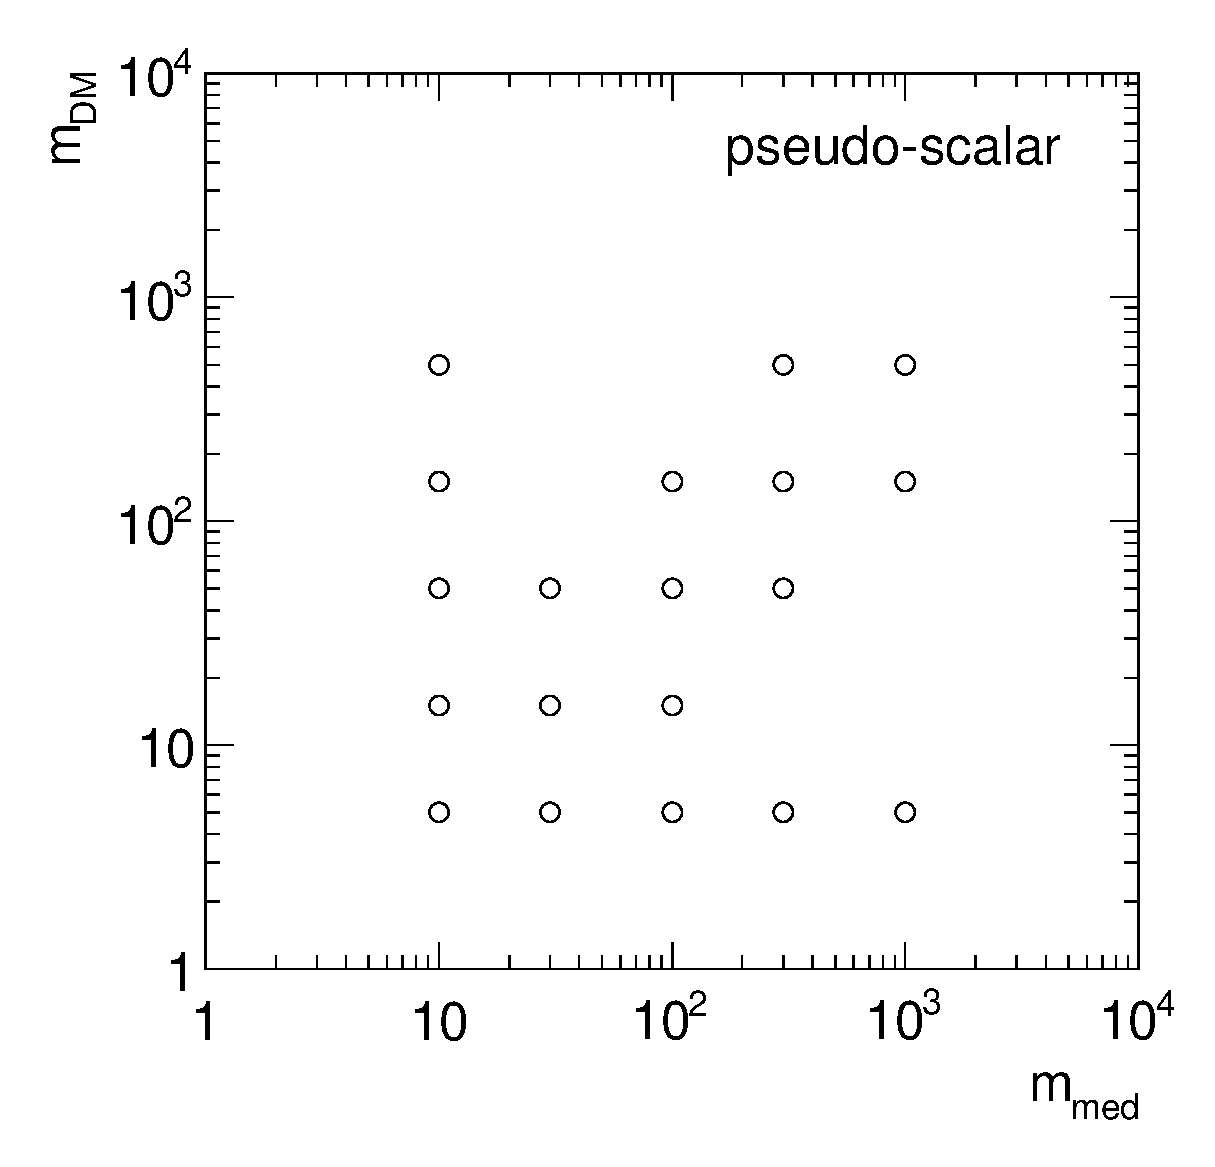
\includegraphics[width=0.95\textwidth]{figures/monojet/grid_P.eps}
% \caption{Proposed parameter grid for scalar and pseudo-scalar mediator in the $\mMed$--$\mDM$ plane.}
% \label{fig:monojet_grid_S}
% \end{figure}

\subsection{Additional considerations for $V+\MET$ signatures}
\label{sub:EW_Scalar}

The discussion of parameters for the model with a color-singlet, \spinzero mediator
parallels that in Section~\ref{subsec:MonojetLikeModels}. 

Even though the sensitivity of mono-boson searches to this model is low and it may not
be in reach of early LHC searches, we recommend to generate this model for W, Z and photon searches 
in order to reproduce the kinematics of contact interaction operators that are further 
described in Section~\ref{sub:EW_EFT_Dim5}, for later reinterpretation.  

%\subsection{Model implementation}
%
%These models are generated at leading
%order with \madgraph 2.2.2, using Pythia8 for the parton shower.
%Parameter cards can be found on the Forum SVN repository~\cite{ForumSVN_EW_DMV}.
%\Todo{Add models and instructions for other final states}.

\subsection{\texorpdfstring{Additional considerations for $t \bar{t}$ and $b \bar{b}$+\MET signatures}{Additional considerations for ttbar/bbbar+\MET signatures}}
\label{subsec:DMHFModels}
\svnidlong
{$HeadURL$}
{$LastChangedDate$}
{$LastChangedRevision$}
{$LastChangedBy$}
\svnid{$Id$}

%As described in Section~\ref{sec:monojet_scalar}, a model with a scalar/pseudoscalar particle 
%mediating the DM-SM interactions is one of the simplest UV completions of our EFT models.  
With the MFV assumption, the top and bottom
quark can play an important  role in the phenomenology.
The scalar and pseudoscalar mediator models predict not only
the monojet process described in Section~\ref{sec:monojet_scalar}, but also production of Dark Matter
in association with top (or bottom) pairs, as illustrated in Fig.~\ref{fig:TTbarPhi}. 
Dedicated searches including jets from heavy flavor quarks in the final state
can be designed for this signature. Another class of simplified models,  
which includes a Dark Matter interpretation among many others, and yields a single
top quark in the final state, is detailed in Appendix~\ref{sec:singletop}. 

\begin{figure}[h!]
\centering
  \unitlength=0.005\textwidth
  \begin{feynmandiagram}[modelTTbarMET]
    \fmfleft{i1,i2}
    \fmfright{o1,o4,o5,o3}
    \fmf{gluon}{i1,v1}
    \fmf{gluon}{i2,v2}
    \fmf{fermion}{o1,v1,v3,v2,o3}
    \fmf{scalar}{v3,v4}
    \fmf{fermion}{o5,v4,o4}
    \fmf{phantom,tension=0,label={$\phi/a$}}{v3,v4}    
    \fmflabel{\Large $g$}{i1}
    \fmflabel{\Large $g$}{i2}
    \fmflabel{\Large $t (b)$}{o1}
    \fmflabel{\Large $\bar t (\bar b)$}{o3}
    \fmflabel{\Large $\chi$}{o4}
    \fmflabel{\Large $\bar \chi$}{o5}    
  \end{feynmandiagram}
%\caption[][\baselineskip]{Representative Feynman
\caption{Representative Feynman
diagram showing the pair production of Dark Matter particles in
association with $t\bar t$ (or $b\bar b$).}
\label{fig:TTbarPhi}
\setfloatalignment{t}
\end{figure}

%\section{Specific models involving $b-$ quarks in the final state}

In addition to the $t\bar t$+DM models illustrated in Fig.~\ref{fig:TTbarPhi}, 
some theoretically motivated scenario (e.g. for high $tan\beta$ in 2HDM in the pMSSM) 
privilege the coupling of \spinzero mediators to down generation quarks.
This assumption motivates the study of final states involving $b$-quarks 
as a complementary search to the $t\bar
t$+DM models, to directly probe the $b$-quark coupling. 
An example of such a model can be found in Ref.~\cite{Buckley:2014fba}
and can be obtained by replacing top quarks with $b$ quarks in Fig.~\ref{fig:TTbarPhi}.
Note that, because of the kinematics features of $b$ quark production relative
to heavy $t$ quark production, a $b\bar b$+DM final state may only yield one
experimentally visible $b$ quark, leading to a mono-$b$ signature in a model that conserves $b$ flavor.

Dedicated implementations of these models for the work of this Forum are available at LO+PS accuracy,
even though the state of the art is set to improve on a timescale beyond that for early Run-2 DM searches
as detailed in Section~\ref{sec:TTBar_implementation}.
The studies in this Section have been produced using a leading order UFO model within \madgraph 2.2.2
~\cite{Alwall:2014hca,Alloul:2013bka,Degrande:2011ua} 
using \pythiaEight for the parton shower. 

\subsubsection{Parameter scan}

%As discussed in Sec.~\ref{subsec:MonojetLikeModels}, the MFV and universal coupling assumptions for \spinzero
%mediators lead to quark mass dependent Yukawa couplings and therefore dominant couplings to top quarks.

The parameter scan for the dedicated $t\bar{t}$+\MET{} searches has been studied in detail to target the production 
mechanism of DM associated with heavy flavor quarks, and shares many details of the scan for the scalar model with a gluon radiation.
The benchmark points scanning the model parameters have been selected to ensure that the kinematic features of the 
parameter space are sufficiently represented. Detailed studies were performed to identify points in the \mdm, 
$m_{\phi,a}$, $\gDM$, $\gq$ (and $\Gamma_{\phi,a}$) parameter space that differ significantly from each other 
in terms of expected detector acceptance. Because missing transverse momentum is the key observable for searches, the 
mediator $p_{T}$ spectra is taken to represent the main kinematics of a model. Another consideration in determining the set 
of benchmarks is to focus on the parameter space where we expect the searches to be sensitive during the 2015 LHC run. 
Based on a projected integrated luminosity of $30\,{\rm fb}^{-1}$ expected for 2015, we disregard model points with a 
cross section times branching ratio smaller than $0.1\,{\rm fb}$, corresponding to a minimum of one expected event 
assuming a 0.1\% efficiency times acceptance. 

The kinematics is most dependent on the masses \mdm and $m_{\phi,a}$. Figure~\ref{fig:scanPhi} 
and~\ref{fig:scanPhiPseudo} show typical dependencies for scalar and pseudoscalar couplings respectively.
Typically, the mediator $p_T$ spectrum broadens with larger $m_{\phi,a}$. 
The kinematics are also different between on-shell ($\mMed>2\mdm$) and off-shell ($\mMed<2\mdm$) mediators as discussed in Section~\ref{sec:monojet_scalar}. 
Furthermore, the kinematic differences in the \MET{} spectrum between scalar and pseudoscalar are larger for light mediator 
masses with respect to heavier mediators. It is therefore important to  
choose benchmark points covering on-shell and off-shell mediators with sufficient granularity, including the
transition region between on-shell and off-shell mediators. %, as inFig.~\ref{fig:scanPhidiag}. 

\begin{figure}[!ht]
  \begin{center}
    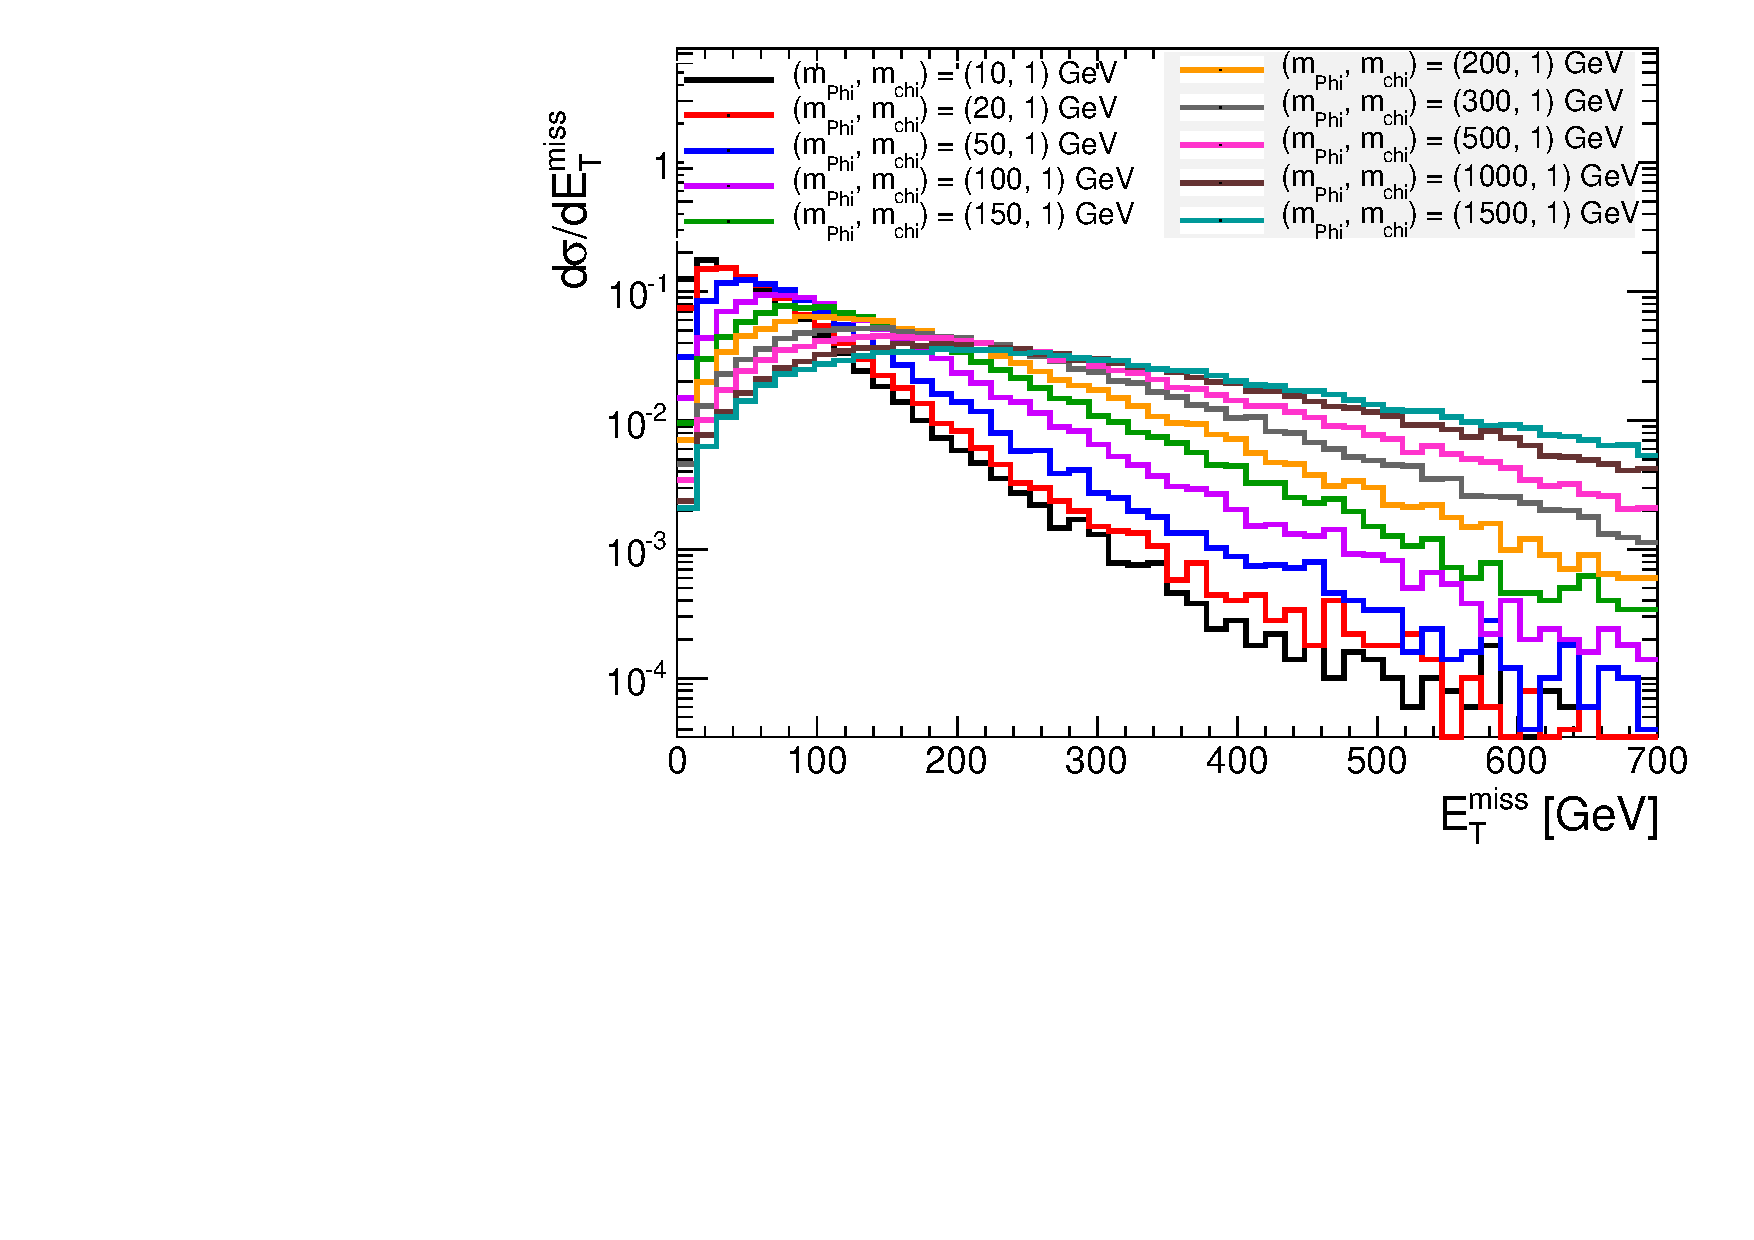
\includegraphics[width=0.95\textwidth]{figures/ttbar/MEt_chi1.pdf}
    \caption{\label{fig:scanPhi} Example of the dependence of the kinematics on the scalar mediator mass in the $t\bar{t}$+\MET{} signature. The Dark Matter mass is fixed to be \mdm=$1 {\rm GeV}$.}
\end{center}
\end{figure}


\begin{figure}[!ht]
  \begin{center}
    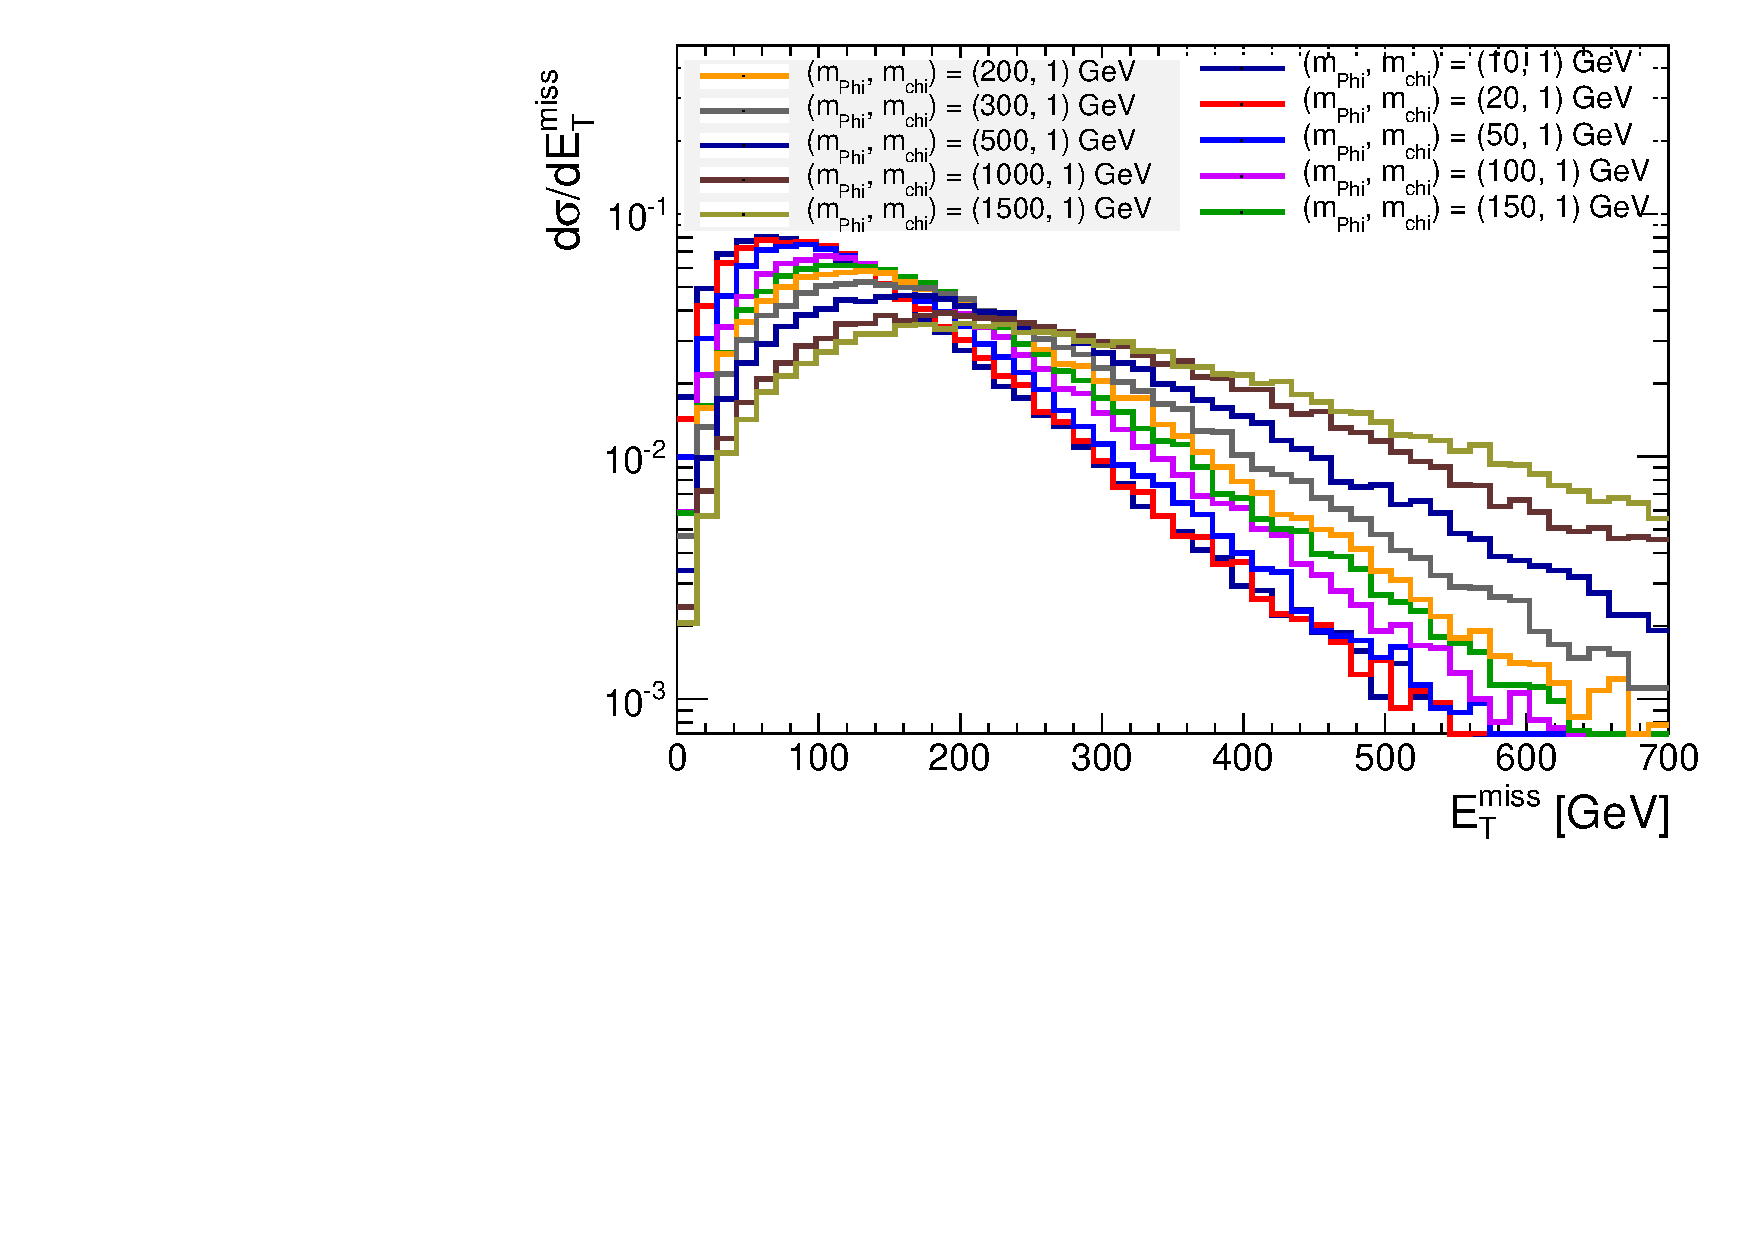
\includegraphics[width=0.95\textwidth]{figures/ttbar/MEt_chi1_pseudo.pdf}
    \caption{\label{fig:scanPhiPseudo} Example of the dependence of the kinematics on the pseudoscalar mediator mass in the $t\bar{t}$+\MET{}. The Dark Matter mass is fixed to be \mdm=$1 {\rm GeV}$. All figures concerning the $t\bar{t}$+\MET{}  signature have been produced using a leading order model within \madgraph 2.2.2, using \pythiaEight for the parton shower.}
\end{center}
\end{figure}

%\begin{figure}[!ht]
%  \begin{center}
%    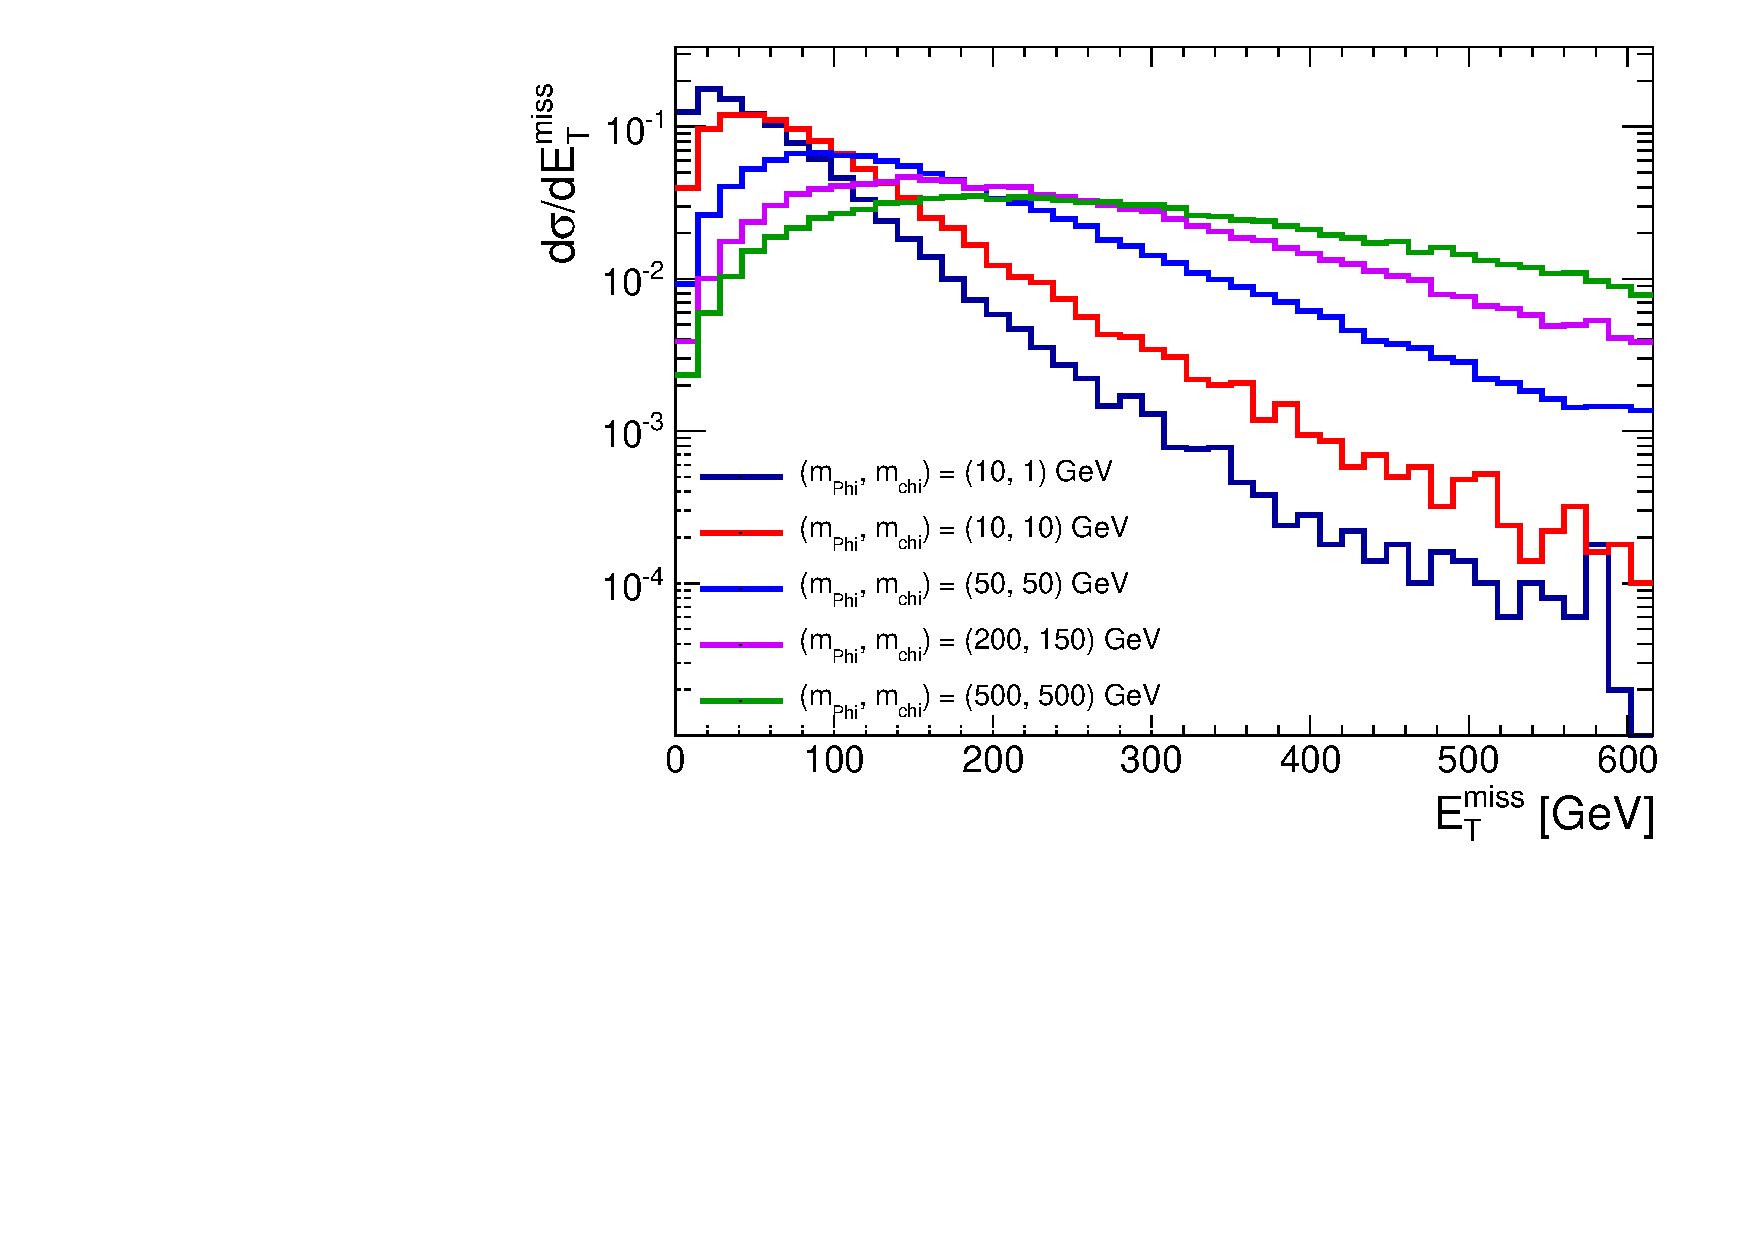
\includegraphics[width=0.95\textwidth]{figures/ttbar/MEt_diagonal_scan.pdf}
%    \caption{\label{fig:scanPhidiag} Example of the dependence of the kinematic for points of the grid proposed in Tab.~\ref{sec:monojet_scalar} close to the $m_{\phi,a} \sim 2m_\chi$ limit.
%    }
%\end{center}
%\end{figure}

Typically only weak dependencies on couplings are observed (see Fig~\ref{fig:widthsmallscan}) where the variation with width of the integral over parton distributions is unimportant. As shown in Section~\ref{sub:parameter_scan_monojet}, for couplings $\sim O(1)$ the width is large enough that the $p_T$ of the mediator is determined mainly by the PDF. 

At large mediator masses ($\sim 1.5\,{\rm TeV}$) or very small couplings ($\sim 10^{-2}$), width effects are significant, but these regimes have production cross sections that are too small to be relevant for $30\,{\rm fb}^{-1}$ and are not studied here. However, with the full Run~2 dataset, such models may be within reach. 

\begin{figure}[!ht]
  \begin{center}
    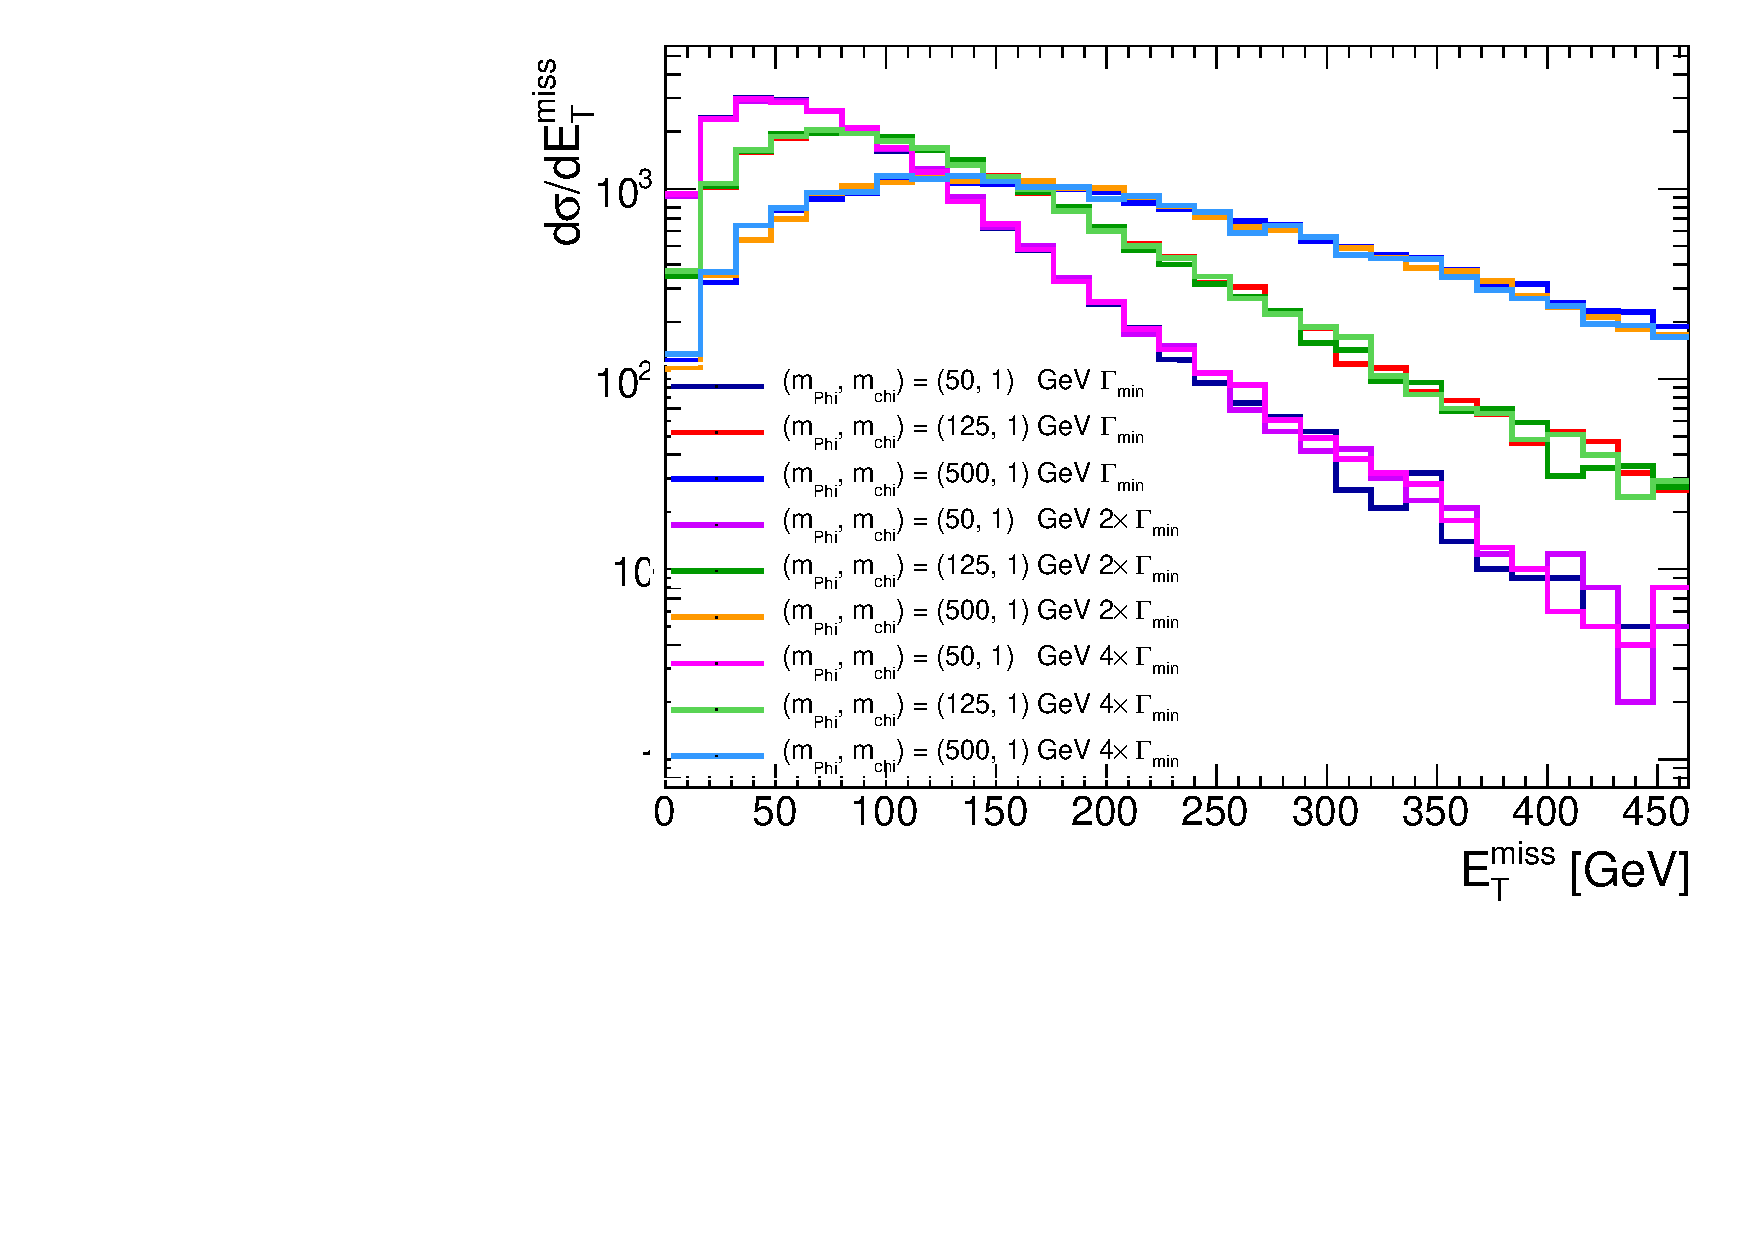
\includegraphics[width=0.95\textwidth]{figures/ttbar/MEt_smallwidth.pdf}
    \caption{\label{fig:widthsmallscan} Study of the dependence of kinematics on the width of a scalar mediator $t\bar{t}$+\MET{}. The width is increased up to four times the minimal width for each mediator and Dark Matter mass combination. 
    }
\end{center}
\end{figure}

Another case where the width can impact the kinematics is when $m_{\phi,a}$ is slightly larger than $2m_\chi$. Here, the width determines the relative contribution between on-shell and off-shell mediators. An example is given in Fig.~\ref{fig:widthlargescan}. As the minimal width choice pursued in this document is the most conservative one, this effect can be neglected in order to reduce the number of benchmark points to be generated. 

%In our recommendations we propose to use for simplicity the minimal width, as this is represents the most conservative choice to interpret the LHC results. 

\begin{figure}[!ht]
  \begin{center}
    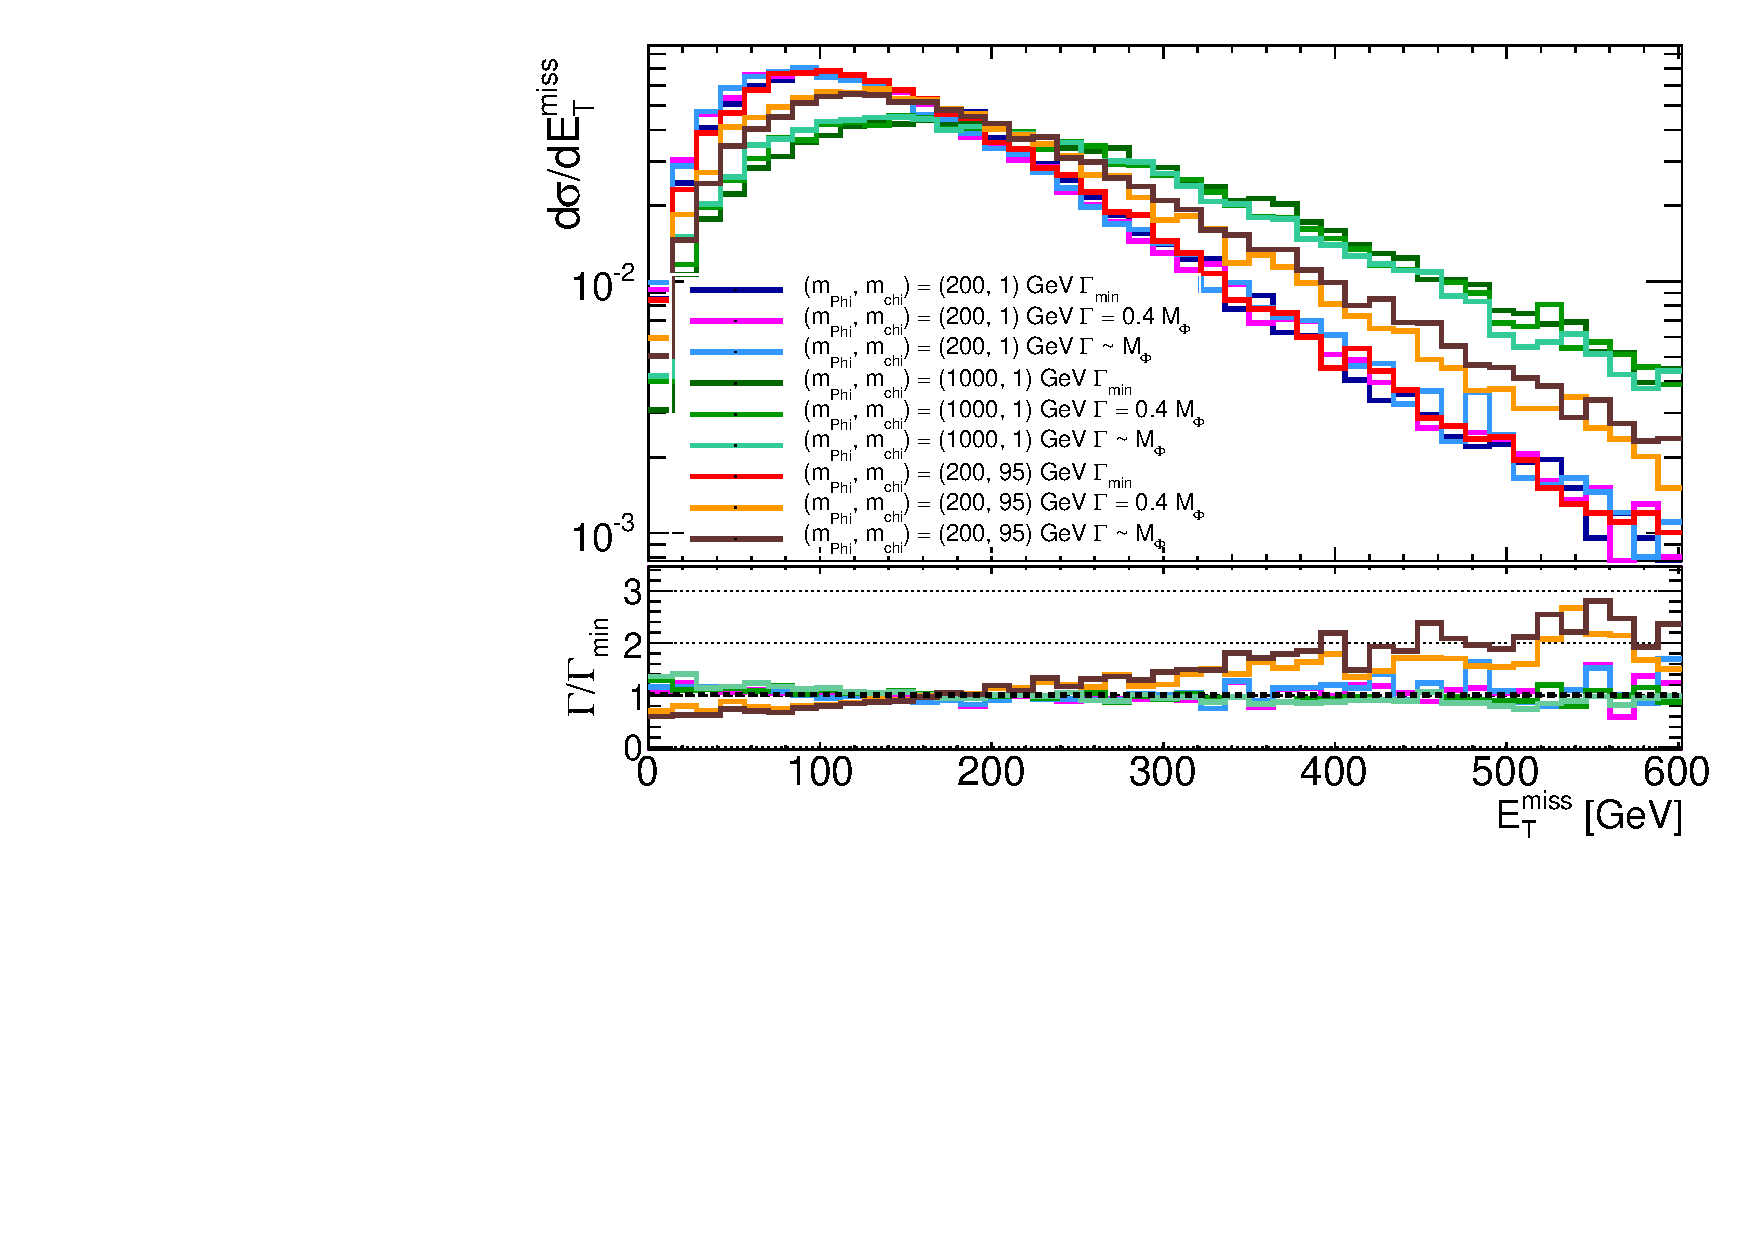
\includegraphics[width=0.95\textwidth]{figures/ttbar/ScalarWidth.pdf}
    \vspace{2mm}
    \caption{\label{fig:widthlargescan} Dependence of the kinematics on the width of a scalar mediator $t\bar{t}$+\MET{}. The width is increased up to the mediator mass. Choices of mediator and Dark Matter masses such that $m_{\phi,a}$ is slightly larger than $2m_\chi$ is the only case that shows a sizeable variation of the kinematics as a function of the width.  
    }
\end{center}
\end{figure}

The points for the parameter scan chosen for this model are listed in Table~\ref{tab:mDMmMedScan_SP}, chosen
to be harmonized with those for other analyses employing the same scalar model as benchmark. 
Based on the sensitivity considerations above, DM masses are only simulated up to 500 GeV (but the 5 TeV mediator point is retained)
leading to a total of 24 benchmark points. However for these searches we recommend to generate and simulate scalar and pseudoscalar
models separately, as the kinematics differs due to the different coupling of the mediator to the final state top quarks in the two cases,
as shown in Figs.~\ref{fig:scanPhi} and ~\ref{fig:scanPhiPseudo}.

Similar studies were performed in the $b \bar b$ case. It was found that they 
show the same weak dependence of the kinematics of the event on the mediator width.
The same benchmark parameters of the $t\bar t$ case could then be chosen.

%%
%[24/05/15 23:48:07] Caterina Doglioni: the plots are made with 5F, while we recommend 4F scheme
%[24/05/15 23:49:04] Caterina Doglioni: even though the relevant parameters do not change 
%(there are some plots due in the appendix for that, albeit with limited statistics), she doesn’t want to put them in 
%and wouldn’t be able to remake them with the right flavor scheme.

% Plots for bbar, if they make it
% Removing these plots as they won't make it last-minute. 
%\Todo{[TODO: The following figures are placeholders for now and will be added later].  If these are supporting material for the MC generation, put in the appendix}.
%
%\begin{figure}
%    \vbox{\hfill}
%    \caption{\label{fig:bbscanPhi} Example of the dependence of the kinematics on the scalar mediator mass. 
%    	The Dark Matter mass is fixed to be $1 {\rm GeV}$.}
%\end{figure}
%
%\begin{figure}[!ht]
%    \vbox{\hfill}
%    \caption{\label{fig:bbscanPhiPseudo} Example of the dependence of the kinematics on the pseudoscalar mediator mass. 
%    	The Dark Matter mass is fixed to be $1 {\rm GeV}$.}
%\end{figure}


%\newthought{Implementation}
%There are some subtleties to the Monte Carlo simulation relevant for
%this case that are discussed in Section~\ref{app:MonojetLikeModels_Appendix}.

%In addition to the considerations discussed in the preceding subsections, very light DM fermions are included ($\mdm=10\,{\rm GeV}$) 
%as this is a region where colliders have a complementary sensitivity to current direct detection experiments. 
% 
% \begin{table}[!ht]
% \centering
% \begin{tabular}{| l | r |}
% \hline
% \multicolumn{1}{|c|}{\mdm (${\rm GeV}$)} & \multicolumn{1}{c|}{$m_{\phi,a}$ (${\rm GeV}$)} \\
% \hline
%  $1$    & $10$, $20$, $50$, $100$, $150$, $200$, $300$, $500$, $1000$, $1500$  \\
%  $10$   & $10$, $20$, $50$, $100$, $150$, $200$, $300$, $500$, $1000$, $1500$  \\
%  $50$   &             $50$, $100$, $150$, $200$, $300$, $500$, $1000$, $1500$  \\
%  $150$  &                          $150$, $200$, $300$, $500$, $1000$, $1500$  \\
%  $500$  &                                               $500$, $1000$, $1500$  \\
% \hline
% \end{tabular}
% \caption{Simplified model benchmarks for $t\bar{t}$+DM production via \spinzero mediators decaying to Dirac DM fermions taking the minimum width presciption for $g_v = \gDM = 1$.}
% \label{tab:ttdm_benchmarks}
% \end{table}
% 


%%%%%%%%%%%%%%%%%
%%%%%%%%%%%%%%%%%
%%%%%%%%%%%%%%%%%
%%%%%%%%%%%%%%%%%
%%%%%%%%%%%%%%%%%
%%%%%%%%%%%%%%%%%
%%%%%%%%%%%%%%%%%

\section{Colored scalar mediator, \tchannel exchange}
\label{sec:monojet_t_channel}
\input tex/TChannelModels.tex

\section{ \Spintwo mediator}
\label{sec:spintwo}

In models with extra dimensions, the Kaluza-Klein excitations of the graviton could also serve as a mediator between the Standard Model and dark sector physics. This kind of model was not studied in the forum and is not included in the recommendations, but it and models such as Ref.~\cite{Lee:2013bua} may warrant further study on a longer timescale. 

% \begin{figure}
%   \centering
%   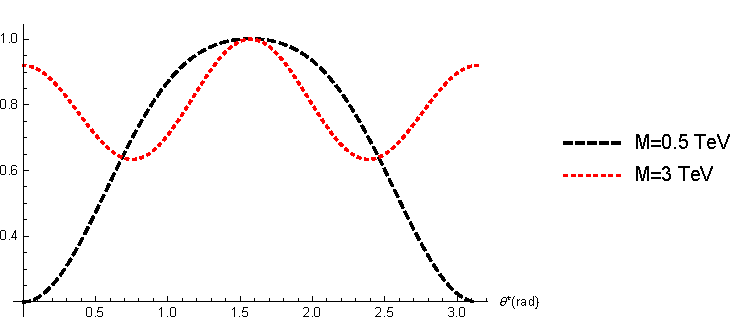
\includegraphics[width=\linewidth]{figures/monojet/comparison_G_mDM10.pdf}
%   \caption{Angular distributions of the total production for 0.5~\tev and 3~\tev graviton mediators for $\mDM=10$~\gev.}
% \end{figure}

% Below a few~\tev in mediator mass, production of a graviton with universal couplings is dominantly gluon-initiated. For heavy mediators, however, up to half of the production occurs through a qq-initiated diagram, leading to a large forward-peaked component of the production \cite{Allanach:2002gn}. For example, Fig.~\ref{fig:gravitoncomparison} shows a calculation of the angular distributions of the total production for 0.5~\tev and 3~\tev graviton mediators in the light WIMP limit ($\mDM=10$~\gev). 

%The proposal for the scan in the $\gq$--$\gDM$ plane is described in the following section.

\section{Presentation of results for reinterpretation of \schannel mediator models}
\label{sec:monojet_scaling}

The aim of the parameter grid optimization done for the \schannel models in the previous sections is to reduce the parameter space that must be simulated.  We then need a procedure for populating the full parameter space by using the simulated grid points.  We recommend doing this as follows:

\begin{itemize}
\item When the dependences on parameters are known, the cross
  sections and efficiencies are general points can be calculated from
  the grid data.
\item In other cases, this information can be obtained by interpolation
  between the grid points.  We have chosen the grid points so that the
  dependence is sufficiently smooth that this will be possible.
\end{itemize}

The results of the scan over the couplings presented in the previous sections indicate that there are no changes in kinematic distributions for different choices of the coupling strengths. This means that the acceptance remains the same in the whole $\gq$--$\gDM$ plane and it is sufficient to perform the detector simulation only for one single choice of $\gq, \gDM$. The resulting truth-level selection acceptance and the detector reconstruction efficiency can then be applied to all remaining grid points in the $\gq$--$\gDM$ plane where only the generator-level cross section needs to be known. This significantly reduces the computing time as the detector response is by far the most CPU-intensive part of the Monte Carlo sample production.
However, the number of generated samples can be reduced even further
if a parameterization of the cross section dependence from one grid point to another exists.
In this section, we describe the details of a cross section scaling procedure that
can be used to reinterpret results for a fixed coupling for \schannel mediator models.

The propagator for the \schannel exchange is written in a Breit-Wigner
form as $\displaystyle \frac{1}{q^2-\mMed^2 + i\mMed\Gamma}$, where $q$ is the momentum transfer calculated from the two partons entering the hard process after the initial state radiation, which is equivalent to the momentum of the Dark Matter pair. %The relative size of the center-of-mass energy defined by the two partons entering the hard process and the mediator mass allows us to classify the production in the following way:
The size of the momentum transfer with respect to the mediator mass allows us to classify the production in the following way:
\begin{itemize}
	\item off-shell production when $q^2 \gg \mMed$ leading to suppressed cross sections,
	\item on-shell production when $q^2 \sim \mMed$ leading to enhanced cross sections,
	\item effective field theory (EFT) limit when $q^2 \ll \mMed$.
\end{itemize}
All three categories can be distinguished in Fig.\,\ref{fig:monojet_MstarMmed} showing the upper limit on the interaction scale $M^{*} \equiv \mMed/\sqrt{\gq\gDM}$ for vector mediator. 
In the case of the off-shell production and the EFT limit, the first and second term in the propagator dominate, respectively, which reduces the dependence on the mediator width. Therefore, in these cases one can approximate the cross section as

\begin{equation}
\sigma \propto \gq^2\gDM^2.
\end{equation}
The on-shell production regime is the most interesting one as it gives the best chances for a discovery at the LHC given the cross section enhancement. The propagator term with the width cannot be neglected in this case and, in the narrow width approximation which requires $\Gamma \ll \mMed$ (this is not necessarily the case in the benchmarks considered in the scans), one can integrate

\begin{equation}
\int \frac{ds}{(s-\mMed^2)^2 + \mMed^2\Gamma^2} = \frac{\pi}{\mMed\Gamma}
\label{eq:monojet_int}
\end{equation}
which further implies the cross section scaling

\begin{equation}
\sigma \propto \frac{\gq^2\gDM^2}{\Gamma}.
\label{eq:monojet_scaling}
\end{equation}
The narrow with approximation is important here as it ensures an integration over parton distribution functions (PDFs) can be neglected. In other words, it is assumed the integrand in Eq.\,\ref{eq:monojet_int} is non-zero only for a small region of $s$, such that the PDFs can be taken to be constant in this range.
By simplifying the dependence of the minimal width on the couplings as $\Gamma \sim \gq^2+\gDM^2$, one can approximate this scaling rule in the extreme cases as follows

\begin{eqnarray}
\sigma &\propto& \frac{\gq^2\gDM^2}{\gq^2+\gDM^2} \xrightarrow{\gq \ll \gDM} \gq^2 \label{eq:monojet_gSM} \\
\sigma &\propto& \frac{\gq^2\gDM^2}{\gq^2+\gDM^2} \xrightarrow{\gq \gg \gDM} \gDM^2 \label{eq:monojet_gDM} \;.
\end{eqnarray}
%However, it is important to keep in mind that there is no simple scaling rule for how the cross section changes with the Dark Matter mass, mediator mass and the mediator width because PDFs matter in such cases as well.
%The only case where there is a simple scaling with mass is if one mass is much smaller than the other mass, in which case the cross section becomes independent of the smaller mass.
However, it is important to keep in mind that this formula omits color and multiplicity factors as well as possible Yukawa suppression, and there is no simple scaling rule for how the cross section changes with the Dark Matter mass and the mediator mass, or for mediators with a large width, because PDFs matter in such cases as well.
Therefore, the scaling procedure outlined above is expected to work only for fixed masses and fixed mediator width, assuming the narrow width approximation applies.


%Figures\,\ref{fig:monojet_width100} and \ref{fig:monojet_width1000} show the minimal width in the $\gq$--$\gDM$ plane for all vector, axial-vector, scalar and pseudo-scalar mediators for $\mMed=100$~\gev and 1000~\gev, respectively, taking $\mDM=10$~\gev.
Figure\,\ref{fig:monojet_width} shows the minimal width over the mediator mass in the $\gq$--$\gDM$ plane for vector and scalar mediators for $\mMed=100$~\gev and 1000~\gev, taking $\mDM=10$~\gev.
The individual colors indicate the lines of constant width, along which the cross section scaling may work for narrow mediators.
The limiting case $\Gamma_{\rm{min}}=\mMed$ defines the upper values of the couplings below which the narrow width approximation can be considered and provides more stringent constraint than the perturbative limit $\gq=\gDM=4\pi$.
For vector and axial-vector mediators, the minimal width is predominantly defined by $\gq$ due to the number of quark flavors and the color factor. %In this case, the scaling follows from Eq.\,\ref{eq:monojet_gDM}.
On the contrary, both the Standard Model and Dark Matter partial width have comparable contributions in case of scalar and pseudo-scalar mediators if the top quark channel is open ($\mMed>2m_t$). However, mostly $\gDM$ defines the minimal width for $\mMed<2m_t$ due to the Yukawa-suppressed light quark couplings.

\begin{figure*}
	\centering
	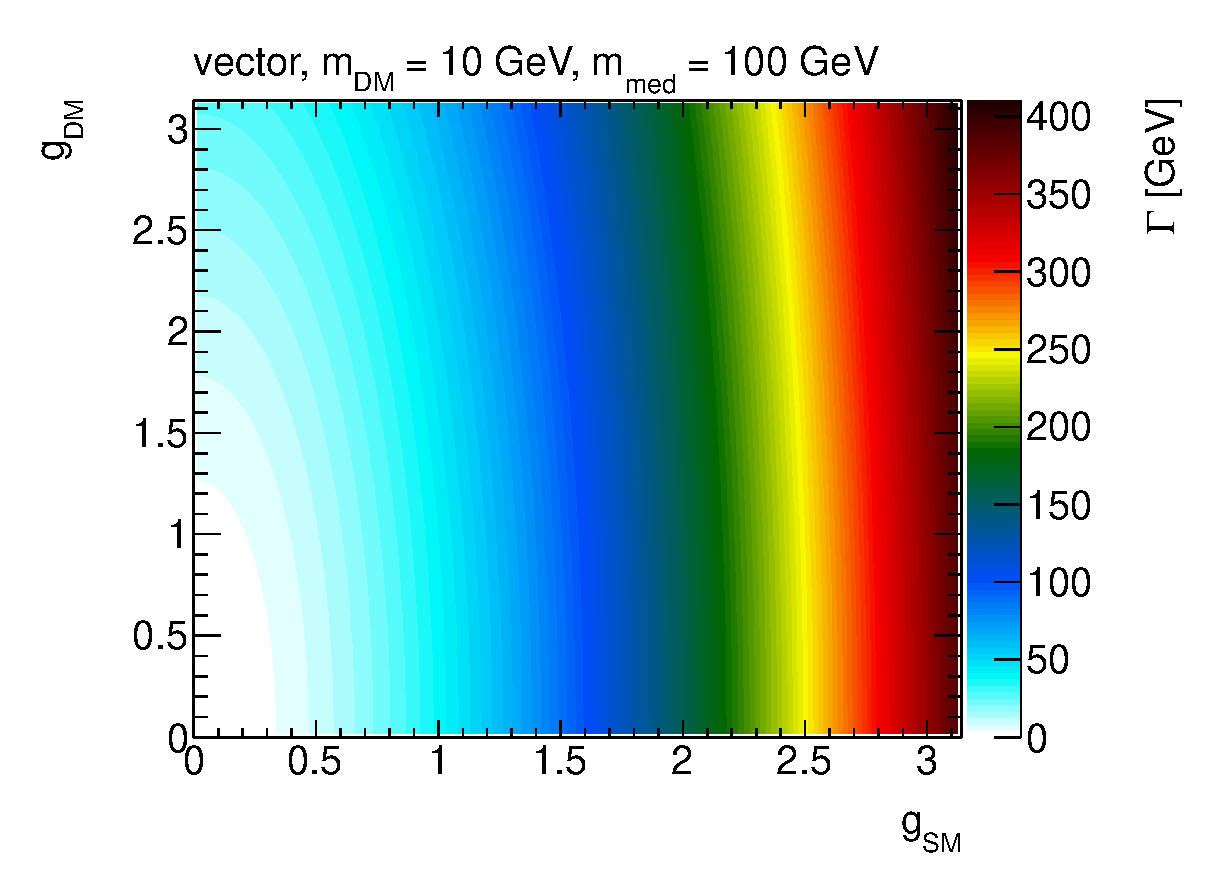
\includegraphics[width=0.49\textwidth]{figures/monojet/constantwidth_V_gg100.eps}
	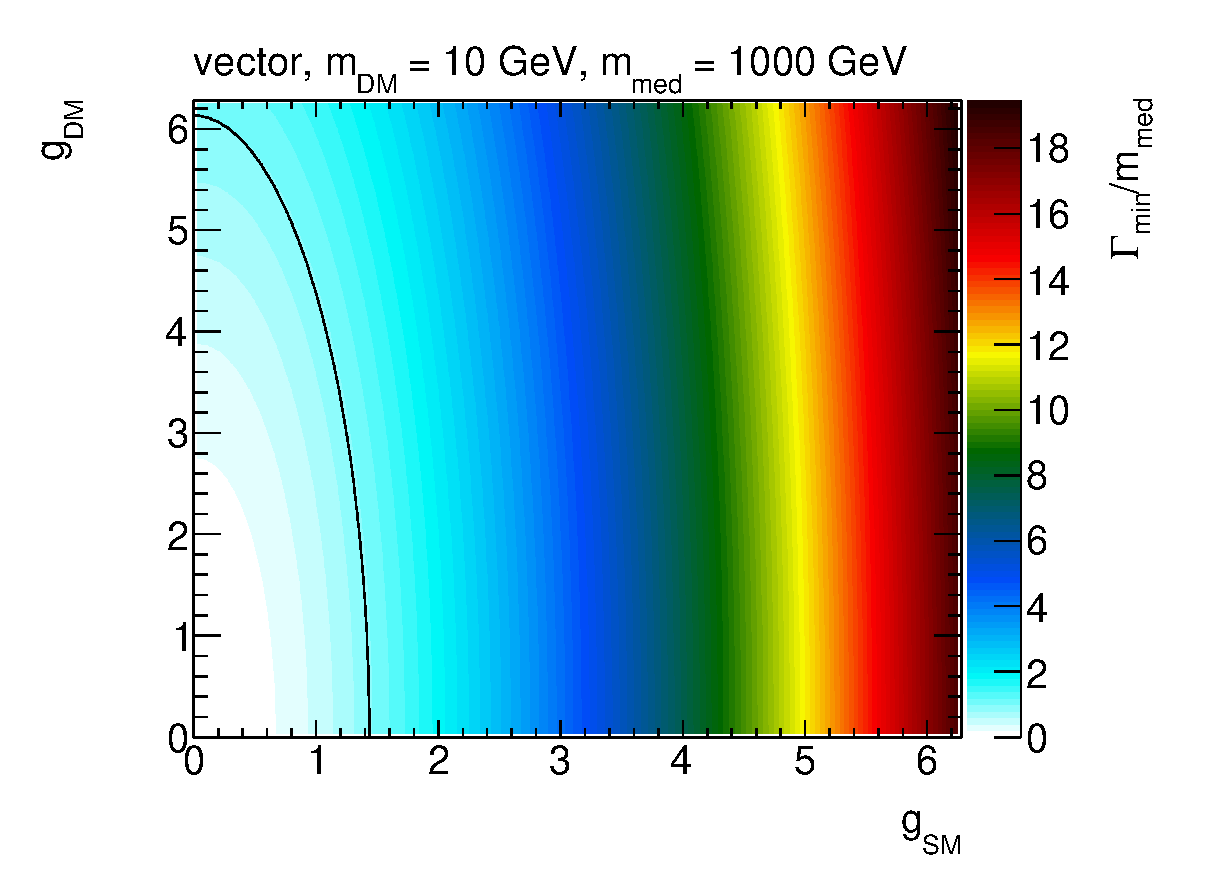
\includegraphics[width=0.49\textwidth]{figures/monojet/constantwidth_V_gg1000.eps}\\
	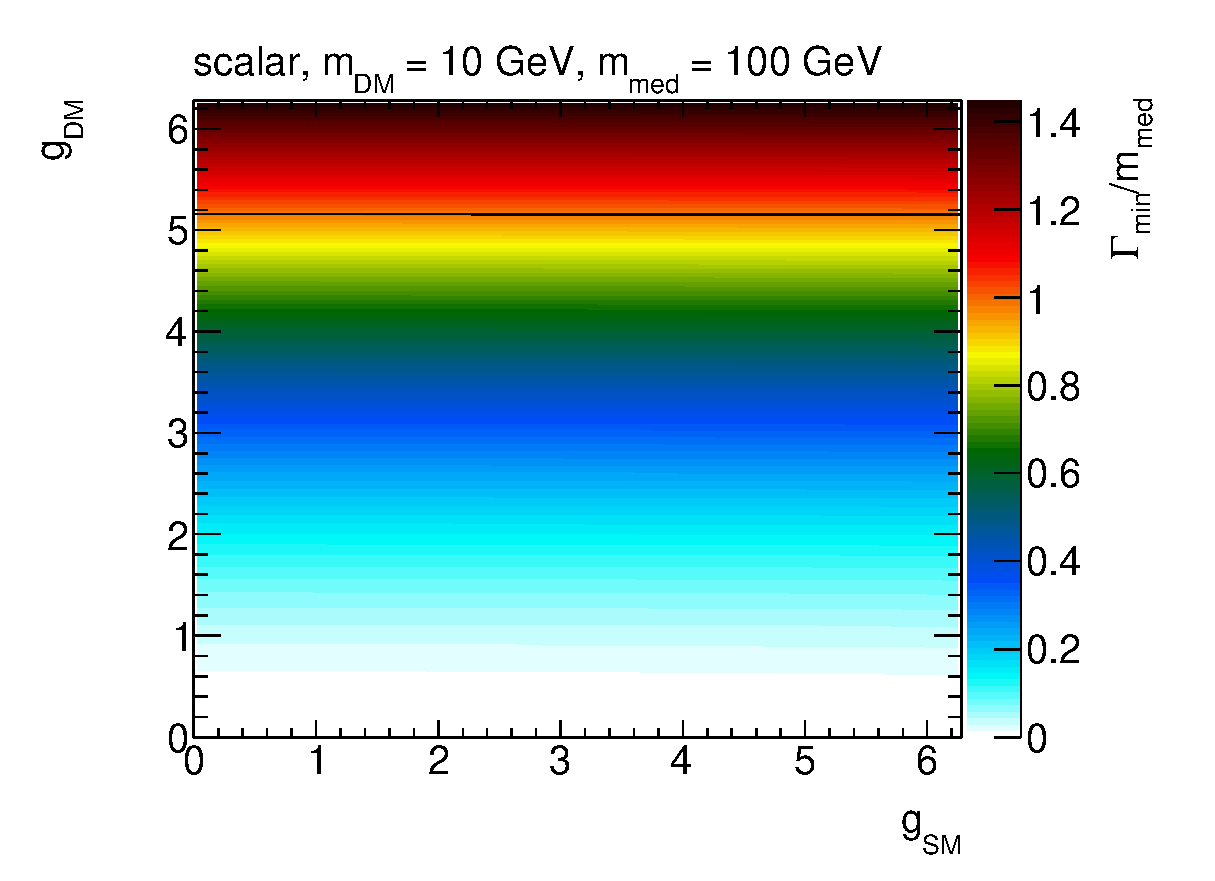
\includegraphics[width=0.49\textwidth]{figures/monojet/constantwidth_S_gg100.eps}
	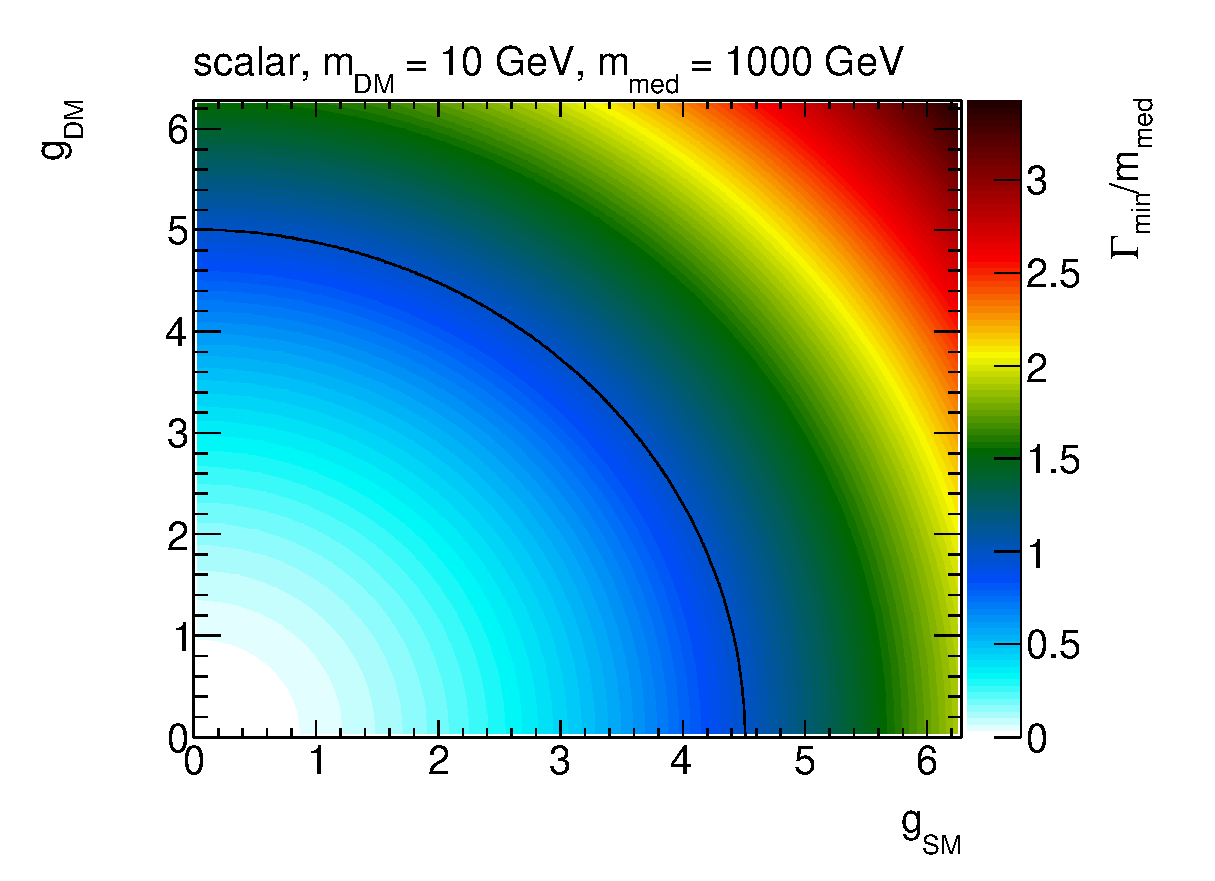
\includegraphics[width=0.49\textwidth]{figures/monojet/constantwidth_S_gg1000.eps}
	\caption{Minimal width over the mediator mass for vector (top) and scalar (bottom) mediators as a function of the individual couplings $\gq$ and $\gDM$, assuming $\mMed=100$~\gev (left) and $\mMed=1$~\tev (right). $\mDM=10$~\gev is considered in all cases.
%		The limiting case $\Gamma_{\rm{min}}=\mMed$ is indicated by the black line.
		Only the cases with $\Gamma_{\rm{min}}<\mMed$ are shown.}
	\label{fig:monojet_width}
\end{figure*}

%\begin{figure}
%	\centering
%	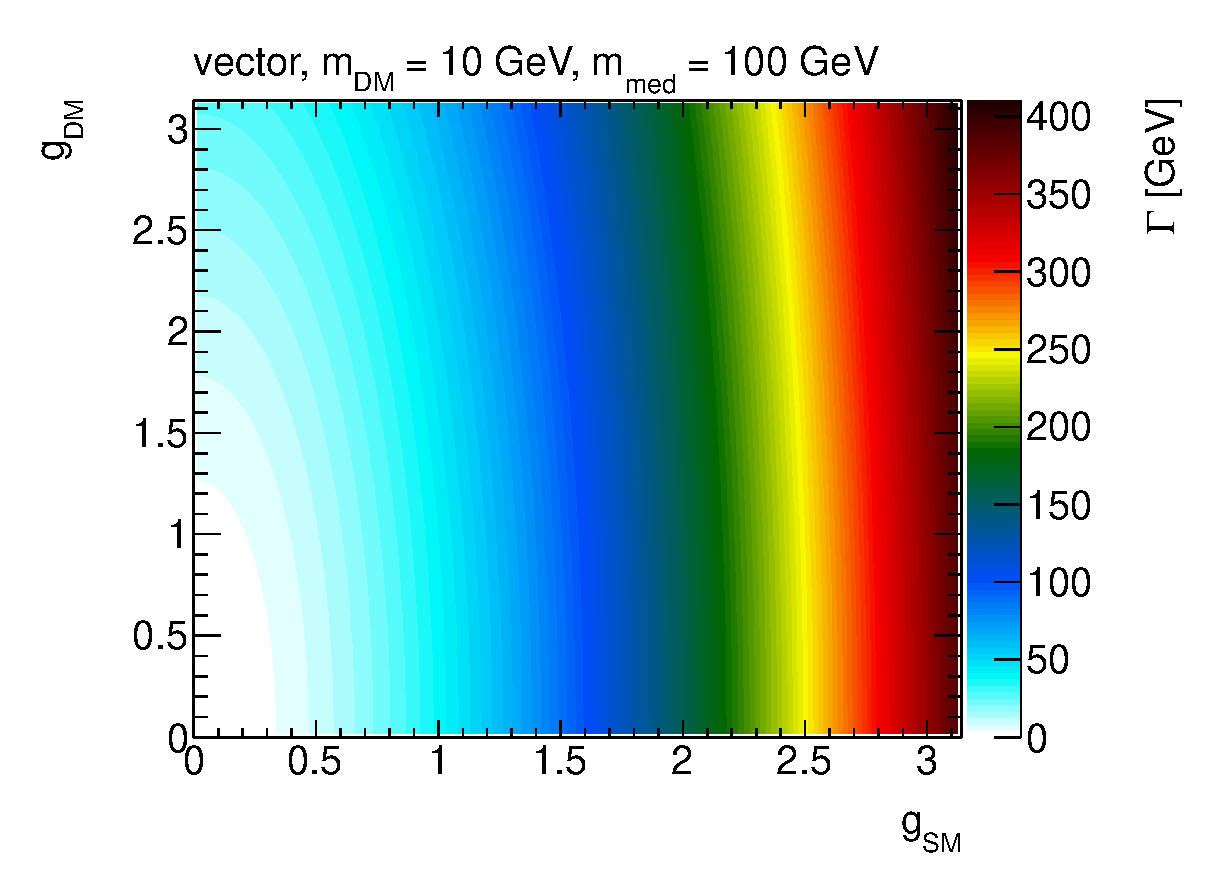
\includegraphics[width=0.95\textwidth]{figures/monojet/constantwidth_V_gg100.eps}
%	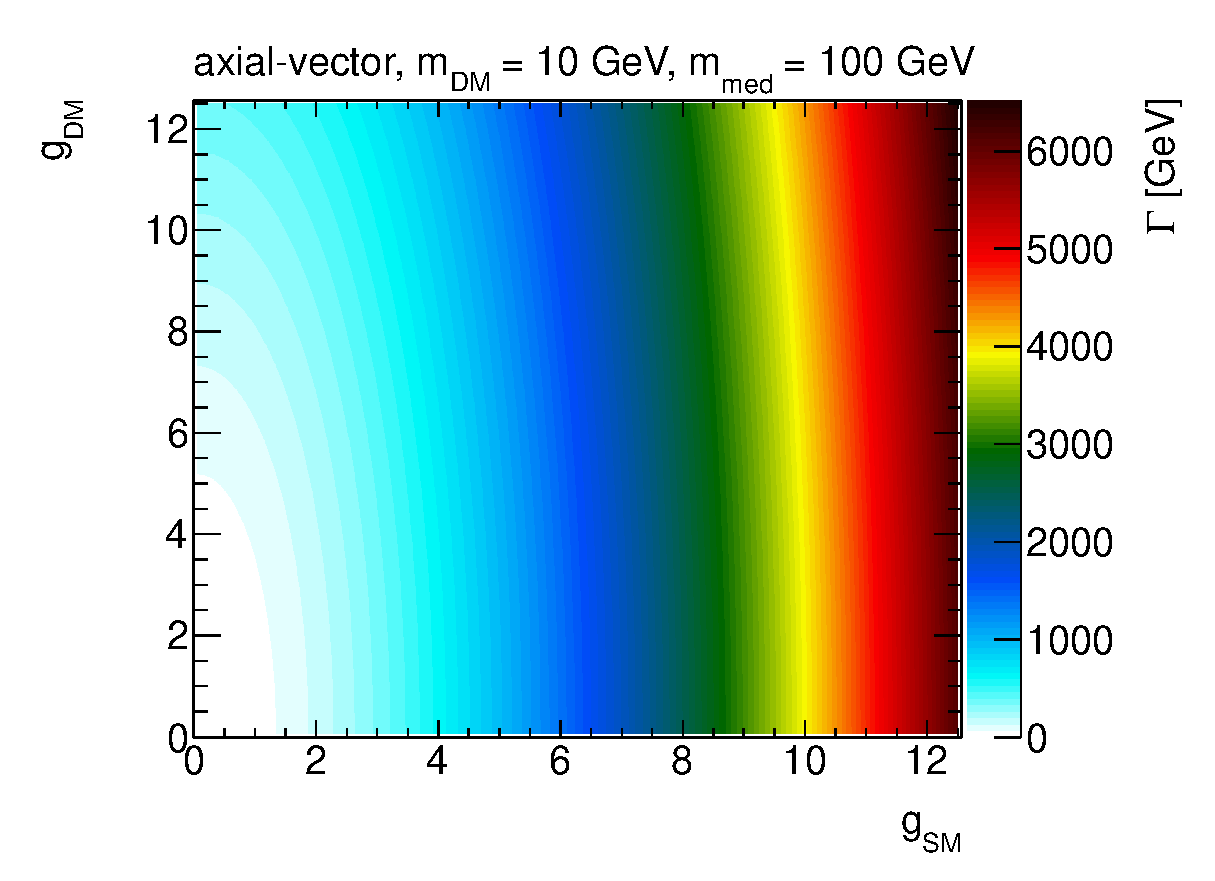
\includegraphics[width=0.95\textwidth]{figures/monojet/constantwidth_A_gg100.eps}\\
%	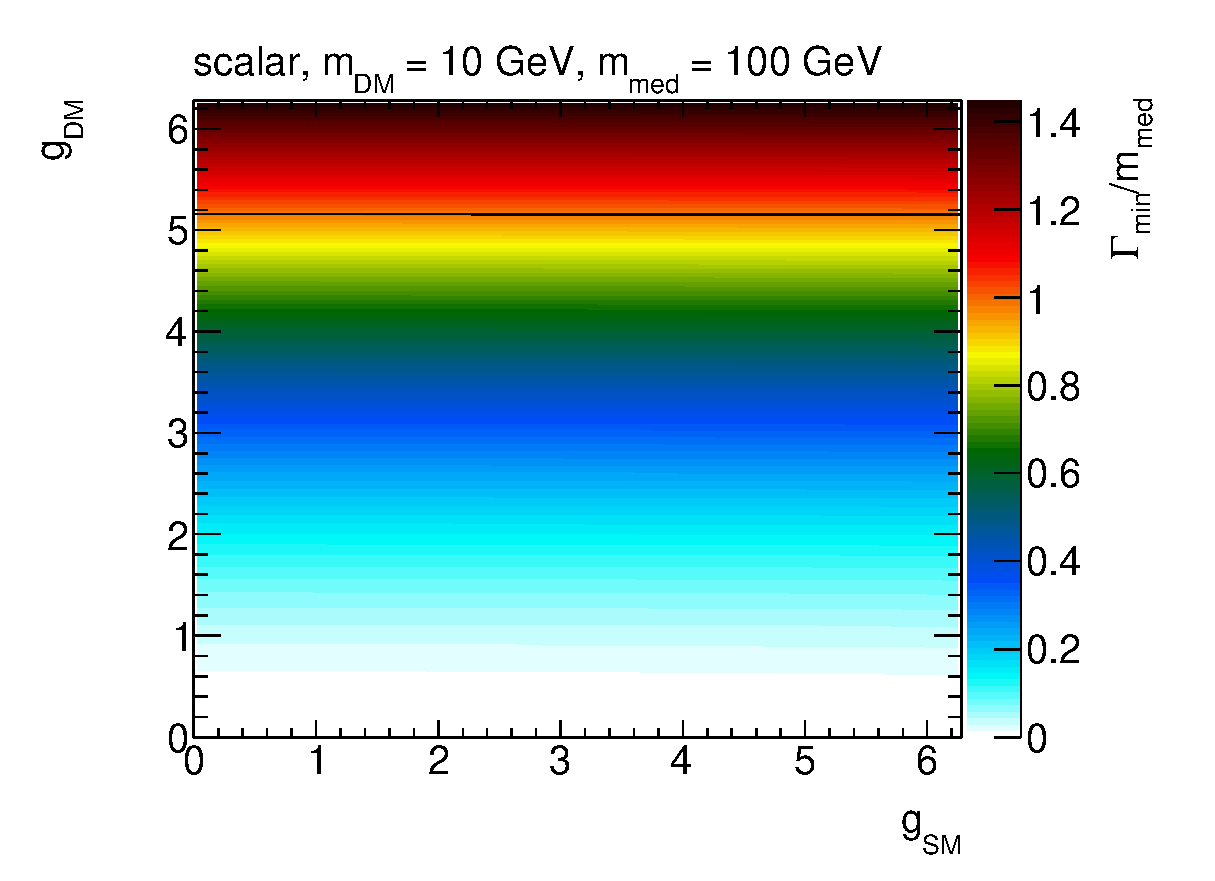
\includegraphics[width=0.95\textwidth]{figures/monojet/constantwidth_S_gg100.eps}
%	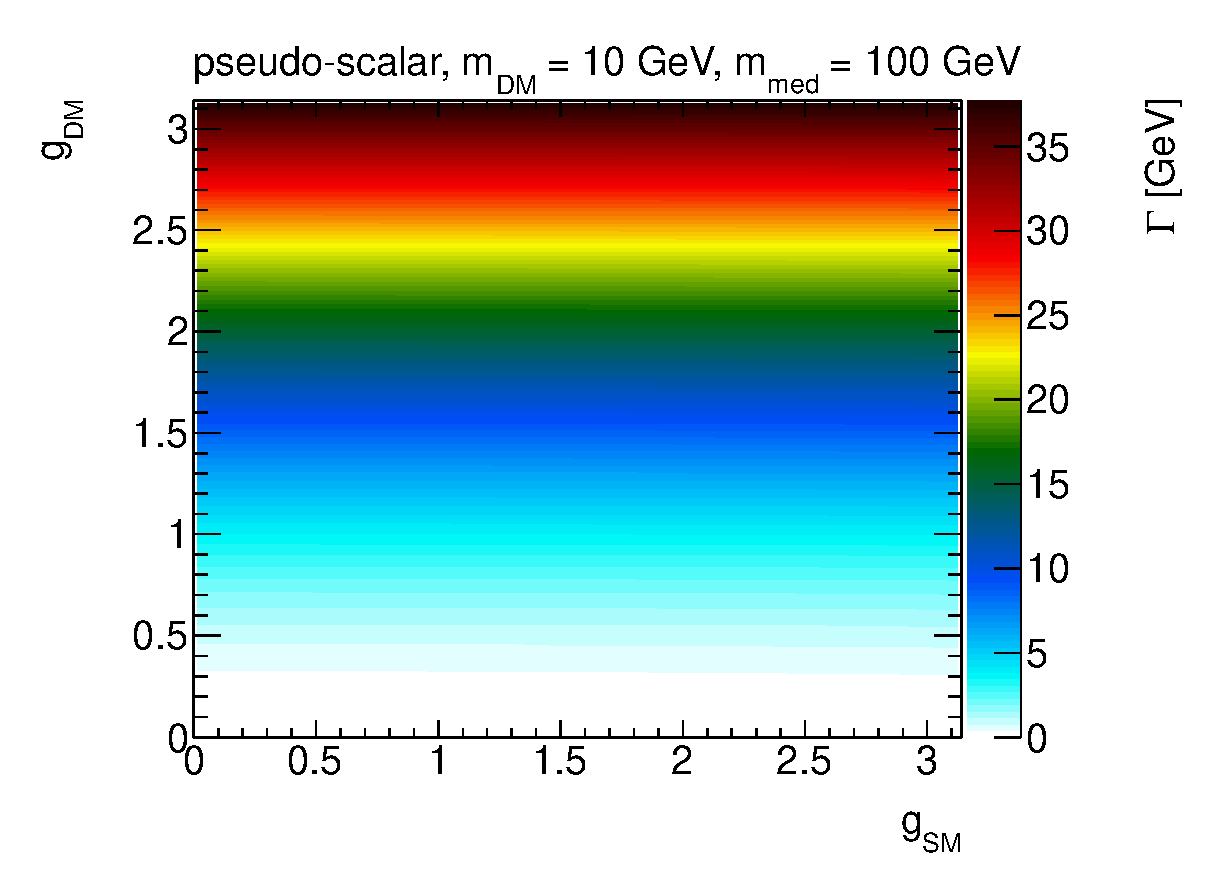
\includegraphics[width=0.95\textwidth]{figures/monojet/constantwidth_P_gg100.eps}
%	\caption{Minimal width over the mediator mass for vector, axial-vector, scalar and pseudo-scalar mediators as a function of the individual couplings $\gq$ and $\gDM$, assuming $\mMed=100$~\gev and $\mDM=10$~\gev.
%		The limiting case $\Gamma_{\rm{min}}=\mMed$ is indicated by the black line.} 
%	\label{fig:monojet_width100}
%\end{figure}
%
%\begin{figure}
%	\centering
%	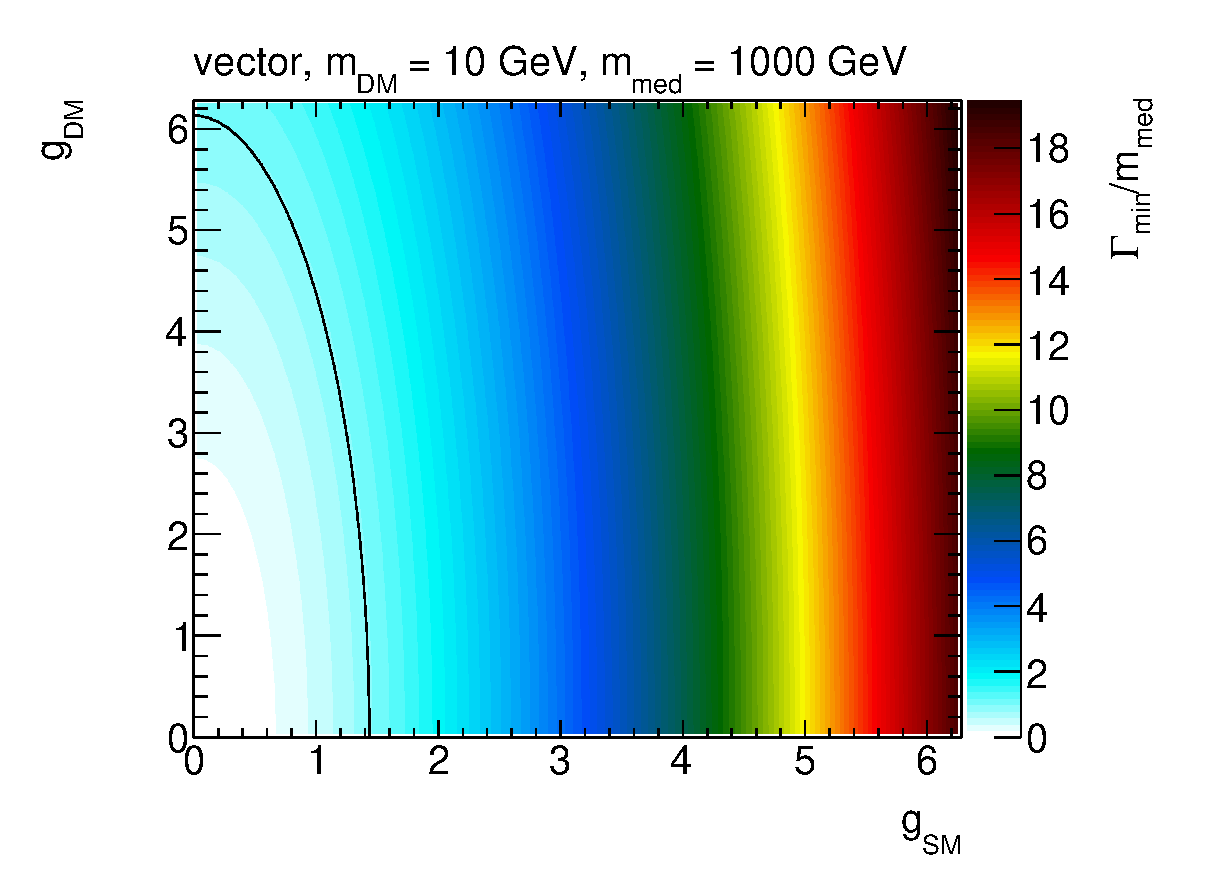
\includegraphics[width=0.95\textwidth]{figures/monojet/constantwidth_V_gg1000.eps}
%	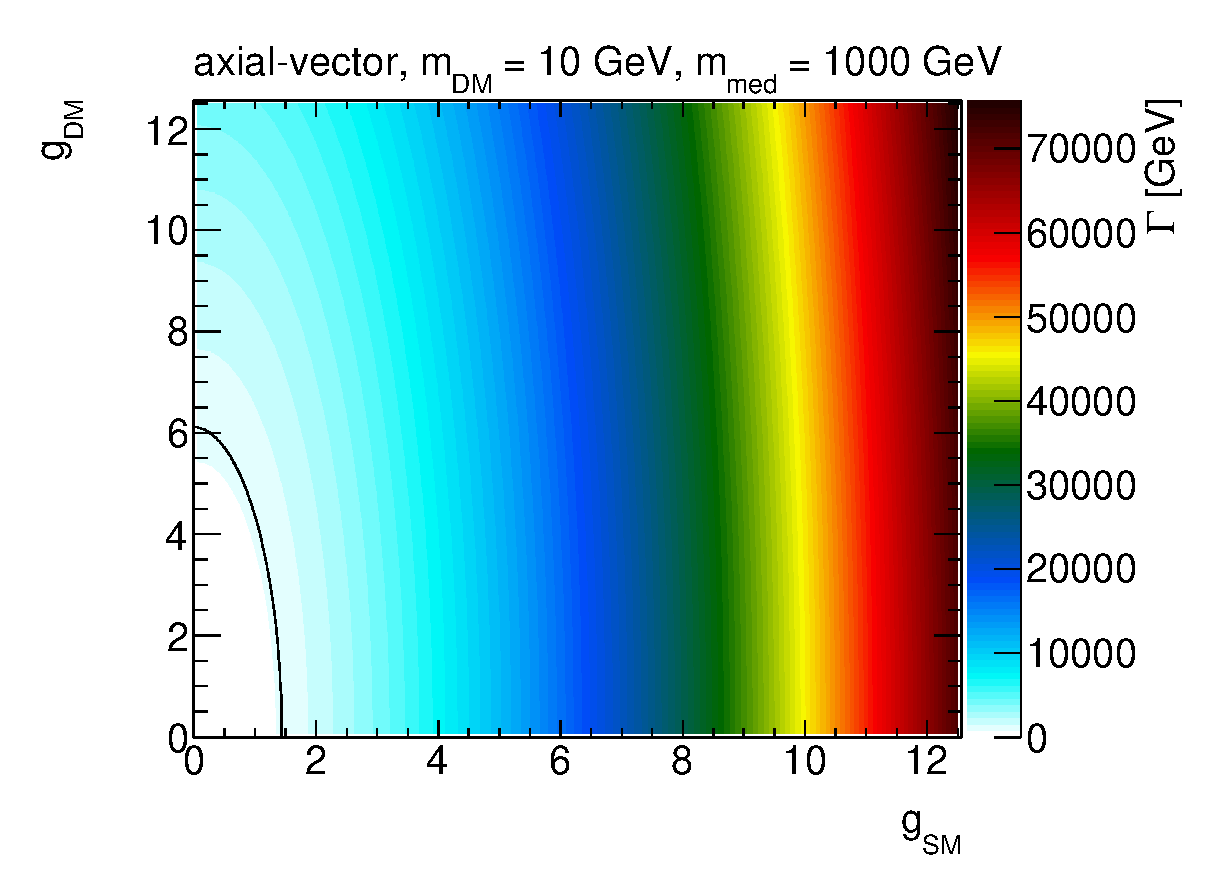
\includegraphics[width=0.95\textwidth]{figures/monojet/constantwidth_A_gg1000.eps}\\
%	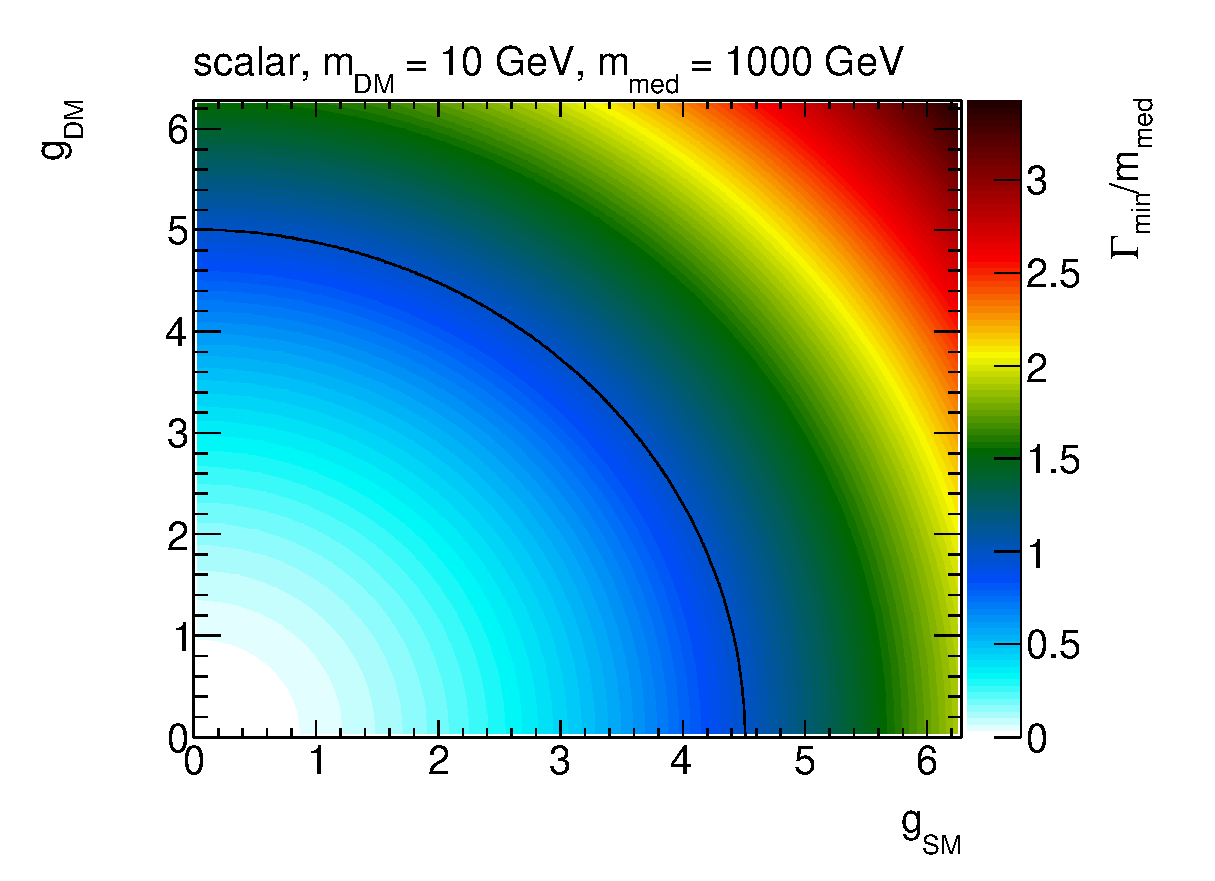
\includegraphics[width=0.95\textwidth]{figures/monojet/constantwidth_S_gg1000.eps}
%	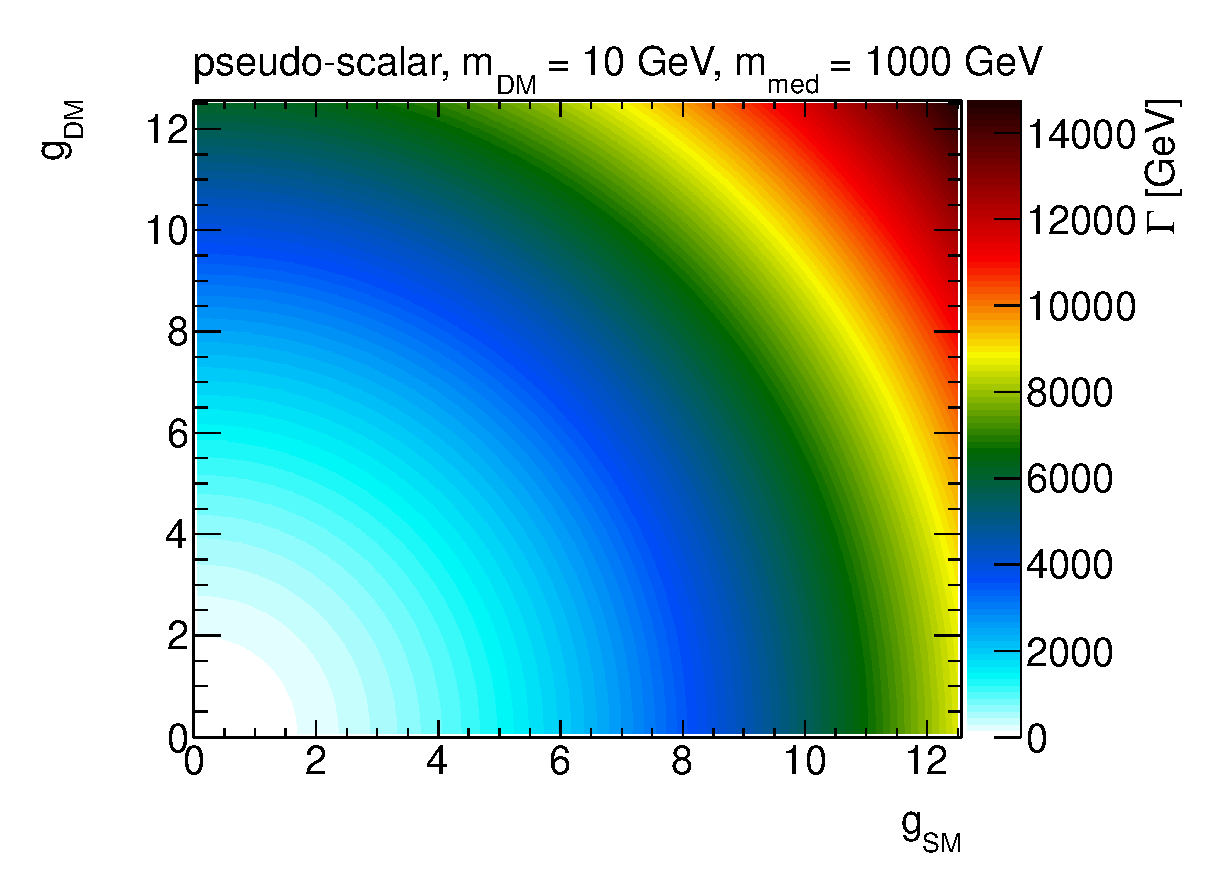
\includegraphics[width=0.95\textwidth]{figures/monojet/constantwidth_P_gg1000.eps}
%	\caption{Minimal width over the mediator mass for vector, axial-vector, scalar and pseudo-scalar mediators as a function of the individual couplings $\gq$ and $\gDM$, assuming $\mMed=1$~\tev and $\mDM=10$~\gev.
%		The limiting case $\Gamma_{\rm{min}}=\mMed$ is indicated by the black line.} 
%	\label{fig:monojet_width1000}
%\end{figure}

%in the plots (gDM = 6, gSM = 1.5 for $V$ and gSM = gDM = 5 for $S$)}


The performance of the cross section scaling is demonstrated in Fig.\,\ref{fig:monojet_scaling} %where two mass points $\mMed=100$~\gev and 1~\tev are chosen with $\mDM=10$~\gev
where two mass points $\mMed=100$~\gev and 1~\tev with $\mDM=10$~\gev are chosen
and rescaled from the starting point $\gq=\gDM=1$ according to Eq.\,\ref{eq:monojet_scaling} to populate the whole $\gq$--$\gDM$ plane. This means the width is not kept constant in this test and this is done in purpose in order to point out deviations from the scaling when the width is altered. For each mass point, the rescaled cross section is compared to the generator cross section and the ratio of the two is plotted.
For the given choice of the mass points, the scaling seems to work approximately within the precision of $\sim20\%$ in the region where $\Gamma_{\rm{min}}<\mMed$.
%For the given choice of the mass points, the scaling seems to work approximately with the precision of $\sim5\%$ for $\Gamma_{\rm{min}}/\mMed<0.1$ and $\sim20\%$ in the region beyond until $\Gamma_{\rm{min}}=\mMed$.
Constant colors indicate the lines along which the cross section scaling works precisely and there is a remarkable resemblance of the patterns shown in the plots of the mediator width. To prove the scaling along the lines of constant width works, one such line is chosen in Fig.\,\ref{fig:monojet_scaling_constwidth} for a scalar mediator, defined by $\mMed=300$~\gev, $\mDM=100$~\gev, $\gq=\gDM=1$, and the rescaled and generated cross sections are found to agree within 3\%.


\begin{figure}
	\centering
	%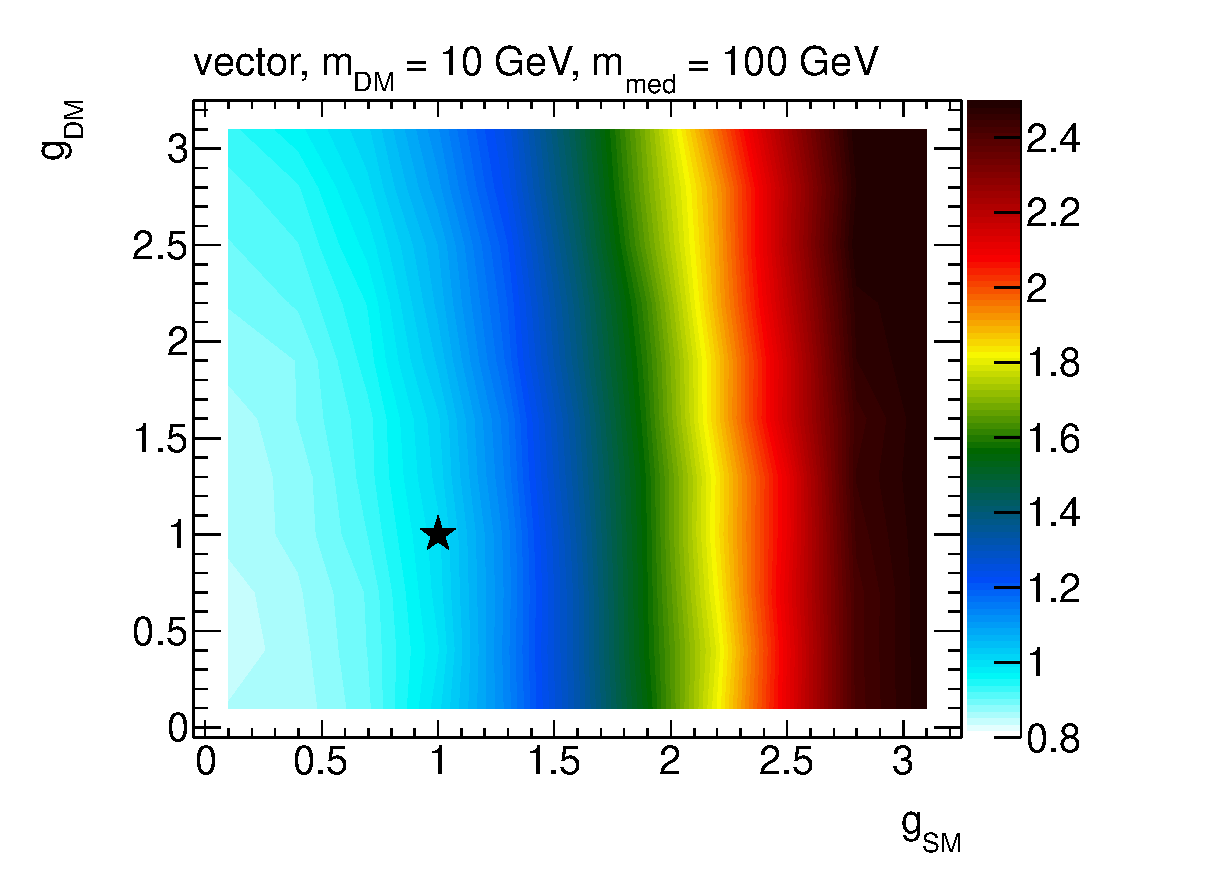
\includegraphics[width=0.95\textwidth]{figures/monojet/scaling_V_10_100.eps}
	%\includegraphics[width=0.95\textwidth]{figures/monojet/scaling_V_10_1000.eps}\\
	\includegraphics[width=0.95\textwidth]{figures/monojet/scaling_S_10_100.eps}
	\includegraphics[width=0.95\textwidth]{figures/monojet/scaling_S_10_1000.eps}\\
	\caption{Ratio of the rescaled and generated cross sections in the $\gq$--$\gDM$ plane. The point at $\gq=\gDM=1$, taken as a reference for the rescaling, is denoted by a star symbol.
		Scalar model with $\mMed=100$~\gev (left) and 1~\tev (right) is plotted for $\mDM=10$~\gev.
		The limiting case $\Gamma_{\rm{min}}=\mMed$ is indicated by a black line and no results are shown beyond.}
	%Vector (scalar) mediator is shown at the top (bottom), the left (right) column corresponds to $\mMed=100$~\gev ($\mMed=1$~\tev). Dark Matter mass of 10~\gev is considered.}
	\label{fig:monojet_scaling}
\end{figure}

%The plots are produced with M_S = 300~\gev, m_chi = 100~\gev, \gSM = \gDM =4
\begin{figure*}
	\centering
	\includegraphics[page=1, trim=310 200 310 200, clip, width=0.49\textwidth]{figures/monojet/rescalingexercise.pdf}
	\includegraphics[page=2, trim=305 195 305 195, clip, width=0.49\textwidth]{figures/monojet/rescalingexercise.pdf}\\
	\includegraphics[page=3, trim=300 190 300 190, clip, width=0.49\textwidth]{figures/monojet/rescalingexercise.pdf}
	\caption{Scaling along the lines of constant width. The line of constant width for $\mMed=300$~\gev and $\mDM=100$~\gev, intercepting $\gq=\gDM=4$ is shown on left. The generated and rescaled cross sections are compared in the middle, the corresponding ratio is shown on right.}
	%TODO ask Uli for the color code
	\label{fig:monojet_scaling_constwidth}
\end{figure*}


\subsection{Proposed parameter grid for cross-section scaling}

We propose to deliver collider results in the $\gq$--$\gDM$ plane using the following prescription, to ease reinterpretation through cross-section scaling:
\begin{itemize}
	\item Since the shapes of kinematic quantities do not change for different couplings, use the acceptance and efficiency for the available $\mDM=50$~\gev, $\mMed=300$~\gev, $\gq=0.25$, $\gDM=1$ grid point from the $\mMed$--$\mDM$ plane for the scalar and pseudo-scalar mediator. In case of the vector and axial-vector mediator, use the grid point $\mDM=150$~\gev, $\mMed=1$~\tev, $\gq=0.25$, $\gDM=1$.
	\item Generate additional samples in order to get generator cross sections only. For scalar and pseudo-scalar mediator, choose $\mDM=50$~\gev, $\mMed=300$~\gev with the following values for $\gq=\gDM$: 0.1, 1, 2, 3. For vector and axial vector mediator, choose $\mDM=150$~\gev, $\mMed=1$~\tev with the following values for $\gq=\gDM$: 0.1, 0.25, 0.5, 0.75, 1, 1.25, 1.5. The upper values are defined by the minimal width reaching the mediator mass. \Todo{Waiting for scalar mediator calculation of perturbativity limit from J. Alcaraz.).}
	\item Rescale the generator cross sections for on-shell resonance production along the lines of constant width in order to populate the whole $\gq$--$\gDM$ plane in the region $\Gamma_{\rm{min}}<\mMed$.
The scaling follows from Eq.\,\ref{eq:monojet_scaling} which for the constant width implies:
\begin{equation}
\sigma' = \sigma \times \frac{\gq'^2\gDM'^2}{\gq^2\gDM^2} \;.
\end{equation}
\end{itemize}

%choose mDM=50, mMed=300, gSM=0.1, gDM={0.1, 1, 2, 3, 4, 5, 6} for S (mMed=GammaMin is reached around 5)
%choose mDM=50, mMed=300, gDM=0.1, gSM={0.1, 0.4, 0.7, 1, 1.3, 1.6, 1.9} for V (mMed=GammaMin is reached around 1.6)
%choose mDM=50, mMed=1000, gDM=0.1, gSM={0.1, 0.4, 0.7, 1, 1.3, 1.6, 1.9} for V (mMed=GammaMin is reached around 1.5)

%choose mDM=50, mMed=300, gSM=gDM={0.1, 1, 2, 3, 4, 5, 6} for S (mMed=GammaMin is reached around 5)
%choose mDM=50, mMed=300, gDM=gSM={0.1, 0.25, 0.5, 0.75, 1, 1.25, 1.5} for V (mMed=GammaMin is reached around 1.5)
%choose mDM=50, mMed=1000, gDM=gSM={0.1, 0.25, 0.5, 0.75, 1, 1.25, 1.5} for V (mMed=GammaMin is reached around 1.4)

\subsection{Rescaling to different mediator width}
\label{paragraph:nonminimalwidth}

In general it is also important to consider a larger mediator width than $\Gamma_{\rm{min}}$ in order to accommodate additional interactions of the mediator with the visible and hidden sector particles~\cite{Buckley:2014fba,Harris:2014hga}. If the narrow width approximation applies, the cross section scaling method described above can be used to reinterpret the results presented for the minimal width, since multiplying the width by factor $n$ is equivalent to changing the coupling strength by factor $\sqrt{n}$, i.e.

\begin{equation}
\sigma(\gq,\gDM, n\Gamma_{\rm{min}}(\gq,\gDM)) \propto \frac{\gq^2 \gDM^2}{\Gamma_{\rm{min}}(\sqrt{n}\gq,\sqrt{n}\gDM)} \;.
\end{equation}
The cross section for the sample with couplings $\gq$ and $\gDM$ and modified mediator width $\Gamma = n\Gamma_{\rm{min}}$ can therefore be rescaled from a sample generated with the minimal width corresponding to the couplings scaled by $\sqrt{n}$ as described in the following formula.

\begin{equation}
\sigma(\gq,\gDM, n\Gamma_{\rm{min}}(\gq,\gDM)) = \frac{1}{n^2} \sigma(\sqrt{n}\gq,\sqrt{n}\gDM,\Gamma_{\rm{min}}(\sqrt{n}\gq,\sqrt{n}\gDM))
\end{equation}
The advantage of doing this is in the fact that no event selection and detector response needs to be simulated since the changes in couplings do not have an effect on the shapes of kinematic distributions.

It should be noted again that this procedure is only useful when the narrow width approximation applies. Care must be taken to ensure that is the case. For example, in the vector and axial-vector cases, one quickly breaks this approximation even for small $n$.

\subsection{\texorpdfstring{Additional considerations for $t \bar{t}$ and $b \bar{b}$+\MET signatures}{Additional considerations for ttbar/bbbar+\MET signatures}}

The cross-section scaling considerations shown in Sec.~\ref{sec:monojet_scaling} still apply for the reactions in the scalar and psuedoscalar models with explicit $b$ and $t$ quarks. Here 
we detail the specific studies done for the  $t\bar t$ model. 

Given that the kinematics are similar for all couplings $g \simeq 1$, we recommend to generate only samples with $\gDM = \gq = 1$. It follows from this that these benchmark points should be a good
approximation for non-unity couplings and for $\gDM \neq \gq$, provided
that the sample is rescaled to the appropriate cross section times
branching ratio.

While the simple scaling function
\begin{equation}
\sigma'\times BR' = [\sigma \times BR]
\times \left( {\gq' \over \gq} \right)^2
\times \left( {\gDM'\over \gDM} \right)^2
\times {\Gamma\over\Gamma'}
\end{equation}
is sufficient for a limited range of coupling values (see Fig.~\ref{fig:xsec_scaling} for example), 
this scaling is only approximate (up to 20\%)  and relies on the narrow width approximation, ignoring PDFs effects. 
%We also choose to provide instead a table of cross section times branching ratio values over a large range of couplings to support interpretation of search results (see the Appendix~\ref{app:TTBar_Xsecs}). The table lists couplings from $g=0.1$ to $g=3.5$, where the upper limit is chosen to be close to but lower than the perturbative limit. 

\begin{figure}[!ht]
	\begin{center}
		\includegraphics[width=0.95\textwidth]{figures/ttbar/xVSwom_mphi_400_mchi_1_proc_S.png}
		\vspace{2mm}
		\caption{\label{fig:xsec_scaling} An example comparing a simple cross section scaling versus the computation from the \madgraph generator, for a scalar $t \bar{t}$+\MET model with $m_{\phi}=400\,{\rm GeV}$, $\mdm=1\,{\rm GeV}$ and all couplings set to unity. In this example, the scaling relationship holds for $\Gamma_{\phi}/m_{\phi}$ below $0.2$, beyond which finite width effects become important and the simple scaling breaks down.}
	\end{center}
\end{figure}


% \section{Scalar models}
% \label{subsec:ScalarModels}
% \section{Spin-0 Mediators}

One of the most straightforward Simplified Models to contemplate is connecting dark matter to the visible sector through a spin-0 mediator, either a scalar or a pseudoscalar. Such models have intriguing connections with Higgs physics, and can be viewed as generalizations of the Higgs Portal to dark matter. The most general scalar mediator models will of course have renormalizable interactions between the Standard Model Higgs and the new scalar $\phi$ or pseudoscalar $A$, as well as $\phi/A$ interactions with electroweak gauge bosons. Such interactions are model-dependent, often subject to constraints from electroweak-precision tests, and would suggest specialized searches which cannot be generalized to a broad class of models (unlike the $\slashed{E}_T$ plus jets searches, for example). As a result, for this class of simplified models with spin-0 mediators, we suggest focusing exclusively on the couplings to fermions, and induced couplings to gluons, leaving the possibilities opened up by couplings to the electroweak sector to the discussion of Higgs Portal dark matter.

In our benchmark models, we will consider two possibilities for the CP assignment of the mediator (scalar and pseudoscalar), and two spin-assignments for the dark matter itself (scalar and fermionic). We provide here the Simplified Model for the interactions of the mediator, the relevant equations for scattering with nucleons and self-annihilation, and a discussion of some important issues in simulating events at the LHC. Throughout, we will assume Minimal Flavor Violation (MFV) for the couplings of the mediators to Standard Model fermions.

\subsection{Fermionic Dark Matter}

Assuming dark matter is a fermion $\chi$ who's interactions with the Standard Model proceed only through a scalar $\phi$ or pseudoscalar $a$, the most general Lagrangian at tree-level are
\begin{eqnarray}
{\cal L}_{{\rm fermion},\phi} & = & {\cal L}_{\rm SM}+i\bar{\chi} \slashed{\partial} \chi + m_\chi \bar{\chi}\chi + \left| \partial_\mu \phi \right|^2+\frac{1}{2}m_\phi^2 \phi^2 + g_\chi \phi \bar{\chi}\chi+ \sum_f \frac{g_v y_f}{\sqrt{2}} \phi \bar{f} f, \label{eq:scalarlag} \\
{\cal L}_{{\rm fermion},a} & = & {\cal L}_{\rm SM}+i\bar{\chi} \slashed{\partial} \chi + m_\chi \bar{\chi}\chi + \left| \partial_\mu a \right|^2+\frac{1}{2}m_a^2 a^2 + i g_\chi a \bar{\chi}\gamma^5 \chi+ \sum_f i \frac{g_v y_f}{\sqrt{2}} a \bar{f}\gamma^5 f. \label{eq:pseudoscalarlag}
\end{eqnarray}
Here, we have made several simplifying assumptions. First, we assume that the coupling to visible-sector fermions is MFV, and proportional to a single universal coupling $g_v$. Thus, the coupling of $\phi$ or $a$ to any flavor of fermion $f$ is set by $g_v \times y_f$, where $y_f$ is the Standard Model yukawa $y_f = \sqrt{2}m_f/v$.\footnote{This normalization for the yukawas assumes $v = 246$~GeV and $y_t \sim 1$.} It is not hard to imagine scenarios that still possess the positive qualities of the MFV assumption but have non-universal $g_v$; for example, couplings only to up-type quarks, or only to leptons. We do not single out any of these options here in our benchmark models, but remind the reader that it is desirable to have experimental constraints sensitive to couplings to different flavors of fermions. Similarly, since there is no ``MFV'' motivation for the structure of dark matter-mediator couplings in the dark sector, and it is of course not known whether the dark matter mass $m_\chi$ is set by only by the Higgs vev $v$ (indeed this would seem to be somewhat unlikely, given the direct detection constraints on dark matter as containing a pure $SU(2)_L$ doublet) we parametrize the dark matter-mediator coupling by $g_\chi$, rather than by some number times a yukawa coupling proportional to $m_\chi$. 

Finally, the most general Lagrangians including new scalars or pseudoscalars should have a potential $V$ containing possible interactions with the Higgs $h$. As stated in the introduction, we choose to take a more minimal set of possible interactions, and leave discussions of the Higgs interactions to the sections on the Higgs Portal.

Given the Lagrangians in Eqs.~\eqref{eq:scalarlag} and \ref{eq:pseudoscalarlag}, the low-energy Lagrangian will develop loop-level couplings between the mediator $\phi/a$ and gluons and photons. This proceeds through loops exactly analogous to the loop-level couplings between the Higgs and gluons and photons. Due to our MFV assumption, as with Higgs physics, the top quark loop will dominate, with the bottom quark playing a minor role. Ignoring all couplings except those to the top, the induced couplings to {\it on-shell} external gluons and photons are
\begin{eqnarray}
{\cal L}_{{\rm loop},\phi} & = & \frac{\alpha_S}{8\pi} \frac{g_v y_t}{v}f_\phi\left(\tfrac{4m_t^2}{m_\phi^2} \right)\phi G^{a,\mu\nu} G^{a}_{\mu\nu} + \frac{\alpha}{8\pi}\left(N_c Q_t^2 \right) \frac{g_v y_t}{v}f_\phi\left(\tfrac{4m_t^2}{m_\phi^2} \right) \phi F^{\mu\nu}F_{\mu\nu} \label{eq:scalarloop} \\ 
{\cal L}_{{\rm loop},a} & = &  \frac{\alpha_S}{4\pi} \frac{g_v y_t}{v}f_a\left(\tfrac{4m_t^2}{m_\phi^2} \right) a G^{a,\mu\nu} \tilde{G}^{a}_{\mu\nu} + \frac{\alpha}{4\pi}\left(N_c Q_t^2 \right) \frac{g_v y_t}{v}f_a\left(\tfrac{4m_t^2}{m_\phi^2} \right) a F^{\mu\nu}\tilde{F}_{\mu\nu} \label{eq:pseudoscalarloop}
\end{eqnarray}
where $\alpha_S$ and $\alpha$ are the QCD and QED fine-structure constants, $N_c = 3$ is the number of quark colors, $Q_t = 2/3$ is the top-quark charge, and the loop integrals are
\begin{eqnarray}
f_\phi(\tau) & = & \left\{\begin{array}{cc} \tau\left(1+(1-\tau)\left[\arcsin\tfrac{1}{\sqrt{\tau}}\right]^{2} \right),  & \tau < 1, \\  \tau\left(1+(1-\tau)\left(-\tfrac{1}{4}\right)\left[ \ln\left(\tfrac{1+\sqrt{1-\tau}}{1-\sqrt{1-\tau}} \right) - i \pi \right]^2 \right), & \tau > 1,\end{array} \right. \\
f_a(\tau) & = & \left\{\begin{array}{cc} \tau\left[\arcsin\tfrac{1}{\sqrt{\tau}}\right]^{2},  & \tau < 1, \\  \tau\left(-\tfrac{1}{4}\right)\left[ \ln\left(\tfrac{1+\sqrt{1-\tau}}{1-\sqrt{1-\tau}} \right) - i \pi \right]^2, & \tau > 1.\end{array} \right.
\end{eqnarray}

{\it It is important to remember the values of the loop-induced couplings shown here are correct only in the limit of on-shell external gauge bosons, and where the internal momenta in the loops are small compared to the top mass. They should not be used in Monte Carlo even-generation with gluon jets that have large $p_T$ when compared to $m_t$, or when the mediators themselves have high $p_T$.} The tree-level couplings of scalar and pseudoscalar mediators to quarks can be used in event-generation through programs like {\tt MadGraph5} as with any other new physics model, and model files are available for these purposes. Correct event generation of scalars/pseudoscalar mediators being produced primarily through the gluon couplings must use more specialized event generation routines, capable of resolving the loop. Such codes include {\tt MCFM} and {\tt Sherpa}, but are not as yet ready for out-of-the-box use in the same manner as {\tt MadGraph}.

These Simplified Models have four free parameters: the universal coupling $g_v$, the dark coupling $g_\chi$, the dark matter mass $m_\chi$, and the mediator mass $m_{\phi}$ or $m_a$. From this, all phenomenology can be calculated. However, one of the critical derived quantities, the mediator width, deserves special discussion. Under the minimal model, the widths for the mediators are given by:
\begin{eqnarray}
\Gamma_\phi & = & \sum_f N_C \frac{y_f^2 g_v^2 m_\phi}{16 \pi} \left(1-\frac{4 m_f^2}{m_\phi^2}\right)^{3/2} + \frac{g_\chi^2 m_\phi}{8 \pi} \left(1-\frac{4 m_\chi^2}{m_\phi^2}\right)^{3/2}  \label{eq:scalarwidth} \\
& & \nonumber + \frac{\alpha_S^2 y_t^2 g_v^2 m_\phi^3}{32 \pi^3 v^2} \left| f_\phi\left(\tfrac{4m_t^2}{m_\phi^2} \right)\right|^2+ \frac{\alpha^2 y_t^2 g_v^2 m_\phi^3}{16\times 9 \pi^3 v^2} \left| f_\phi\left(\tfrac{4m_t^2}{m_\phi^2} \right)\right|^2 \label{eq:pseudoscalarwidth} \\
\Gamma_a & = & \sum_f N_C \frac{y_f^2 g_v^2 m_a}{16 \pi} \left(1-\frac{4 m_f^2}{m_a^2}\right)^{1/2} + \frac{g_\chi^2 m_a}{8 \pi} \left(1-\frac{4 m_\chi^2}{m_a^2}\right)^{1/2}  \\
& & \nonumber + \frac{\alpha_S^2 y_t^2 g_v^2 m_a^3}{8 \pi^3 v^2} \left| f_a\left(\tfrac{4m_t^2}{m_\phi^2} \right)\right|^2+ \frac{\alpha^2 y_t^2 g_v^2 m_a^3}{4\times 9 \pi^3 v^2} \left| f_a\left(\tfrac{4m_t^2}{m_a^2} \right)\right|^2 
\end{eqnarray}
Here, the first term in each width corresponds to the decay into Standard Model fermions (the sum runs over all kinematically available fermions, $N_C = 3$ for quarks and $N_C = 1$ for leptons). The second term is the decay into dark matter (assuming that this decay is kinematically allowed), and the last two terms correspond to decay into gluons and photon pairs. The factor of 2 between the decay into Standard Model fermions and into dark matter is a result of our choice of normalization of the yukawa couplings.

In colliders, if the mediator is produced on-shell, as is the primary mode of dark matter production when $m_\chi < m_{\phi/a} /2$ and $m_{\phi/a} \ll \sqrt{\hat{s}}$ (where $\sqrt{\hat{s}}$ is some characteristic c.o.m. at the collider in question), the cross section of dark matter production will be proportional to the branching ratio into dark matter. The total production of the mediator will go as $g_v^2$, and the decay into invisible dark matter will be $\propto g_\chi^2/\Gamma_{\phi/a}$, with the appropriate kinematic factors. This confounds the easy factorization of limits on the four-dimensional parameter space, since while the total cross section will have an overall dependence on the product $g_\chi^2 \times g_v^2$, it will also depend on $\Gamma_{\phi/a}$, which even in the minimal model depends on the sum of $g_\chi^2$ and $g_v^2$ (with kinematic factors inserted). 

In addition, as this is a Simplified Model, it is possible that the mediator can decay into additional states present in a full theory that we have neglected. For example, the mediator could decay into additional new charged particles which themselves eventually decay into dark matter, but with additional visible particles that would move the event out of the selection criteria of monojets or similar missing energy searches. Thus, the widths calculated in Eqs.~\eqref{eq:scalarwidth} and \eqref{eq:pseudoscalarwidth} are lower bounds on the total width. 

As a result of these issues, the width of the mediator is often treated as an independent variable in Simplified Models with $s$-channel production of dark matter. Fortunately, for on-shell production, the effect of changing the width is only a rescaling of the total event rate assuming that $\Gamma_{\phi/a} < m_{\phi/a}$ \cite{Buckley:2014fba}, which is a necessary condition for a valid weakly coupled theory. As a result, changing the width just rescales the total event rate at colliders. In the case when the dark matter is produced through an off-shell mediator, the width is not relevant. We therefore recommend that experimental and theoretical bounds on $s$-channel models make the assumption that the width is minimal, set by Eqs.~\eqref{eq:scalarwidth} or \eqref{eq:pseudoscalarwidth}, and treat it as a dependent quantity, rather than an additional free parameter.

Furthermore, as we are dealing with a 4D parameter space, it is necessary to consider how to reduce the parameter space to display results which can be compared between experiments and with theory. Clearly, the dependence of the constraints from experiments on the masses $m_\chi$ and $m_{\phi/a}$ cannot be suppressed, as the bounds will have non-trivial kinematic dependences on the masses. This leaves the couplings $g_\chi$ and $g_v$. The most straightforward assumption to make is to set $g_\chi = g_v$. This has the somewhat unfortunate result of making certain types of experimental results appear more effective than others. For example, with $g_\chi = g_v$, we expect the mediator branching ratio to dark matter to completely dominate over the visible channels, unless the top channel is kinematically allowed. This would make resonance searches in visible channels for the mediator appear to be uncompetitive. However, some choice must be made, and setting the two couplings equal to each other is perhaps the simplest.

We now turn to the constraints on these models from non-collider experiments: thermal relic abundances, indirect detection, and direct detection. The first two results can be considered together, as they depend on the same set of annihilation cross sections.

\paragraph{Thermal Cross Sections}

The thermally-average annihilation of dark matter through the spin-0 mediators can be calculated from the Simplified Model Eqs.~\eqref{eq:scalarlag} and \eqref{eq:pseudoscalarlag}. The resulting cross sections for annihilation into Standard Model fermions, as a function of the dark matter temperature $T$ are
\begin{eqnarray*}
\langle \sigma v \rangle(\chi\bar{\chi} \to \phi^* \to f\bar{f}) & = & N_c \frac{3 g_\chi^2 g_v^2 y_f^2 (m_\chi^2 - m_f^2)^{3/2}}{8\pi m_\chi^2\left[ (m_\phi^2 - 4m_\chi^2)^2 + m_\phi^2\Gamma^2_\phi \right]} T, \label{eq:scalarthermal} \\
\langle \sigma v \rangle(\chi\bar{\chi} \to a^* \to f\bar{f}) & = & N_c \frac{g_\chi^2 g_v^2 y_f^2 }{4\pi \left[ (m_a^2 - 4m_\chi^2)^2 + m_a^2\Gamma^2_a \right]} \left[ m_\chi^2 \sqrt{1-\frac{m_f^2}{m_\chi^2}} + \frac{3m_f^2}{4m_\chi \sqrt{1-\frac{m_f^2}{m_\chi^2}}} T \right].  \label{eq:pseudoscalarthermal} \\
\end{eqnarray*}
Notably, the scalar mediators do not have a temperature-independent contribution their annihilation cross section, while pseudoscalars do. As $T \propto v^2$, where $v$ is the dark matter velocity, there is no velocity-independent annihilation through scalars. As, in the Universe today, $v \lesssim 10^{-3}$, this means there are no non-trivial constraints on dark matter annihilation from indirect detection in the scalar mediator model. 

The pseudoscalar model, on the other hand, does have relevant constraints from indirect detection. These can be obtained from Eq.~\ref{eq:pseudoscalarthermal} by setting $T \to 0$, and considering annihilation into the relevant Standard Model channel(s). Most constraints from indirect detection are written in terms of a single annihilation channel, and so the constraints for the full Simplified Model (with multiple annihilation channels open) require some modification of the available results. Good estimates can be obtained by considering the most massive fermion into which the dark matter can annihilate (typically the $b$ or $t$ quark), as this will tend to dominate the annihilation cross section. Note that, outside of resonance, the width is relatively unimportant to the indirect detection constraints.

The thermal relic calculation requires the same input cross sections as the indirect detection. Here, the cross sections are summed over all kinematically available final states, and can be written parametrically as
\[
\langle \sigma v\rangle = a + bT. 
\]
The thermal relic abundance of dark matter is then
\begin{equation}
\Omega_\chi h^2 = \frac{1.04\times 10^9~\mbox{GeV}}{m_{\rm Planck}}\frac{x_f}{\sqrt{g_\star}}\frac{1}{a+b m_\chi x_f^{-1}},
\end{equation}
where $x_f \sim 25$ is $m_\chi$ over the freeze-out temperature, and $g_{\rm star}$ is the number of degrees of freedom active at the time of freeze-out. For reasonable early Universe parameters, the correct relic abundance occurs when
\begin{equation}
3 \times 10^{-26}~\mbox{cm$^3$/s} = 2.57 \times 10^{-9}~\mbox{GeV}^{-2} = a + \frac{b m_\chi}{x_f}.
\end{equation}
Keep in mind that these equations require some modification when the dark matter-mediator system is on resonance. Further, recall that we do not know dark matter is a thermal relic, or that the only annihilation process in play in the early Universe is through the mediator. Therefore, while it is appropriate to compare the sensitivity of experimental results to the thermal cross section, this is not the only range of parameters of theoretical interest.

\paragraph{Direct Detection}

As noted previously, the scalar mediator model has no indirect detection constraints, while the pseudoscalar does. The situation is reversed in direct detection: the pseudoscalar mediator has no velocity- or momentum-unsuppressed interactions with nucleons, while the scalar mediator induces a spin-independent scattering cross section. These constraints are very powerful compared to the present collider bounds, especially when $m_\chi > 10$~GeV. As with indirect detection, for weakly coupled theories, the direct detection bounds are relatively independent of the width. 

For the scalar mediator model, the interaction with direct detection nuclear targets is (to good approximation) isospin-conserving. Therefore, the bound on scattering with nucleons can be applied to either the dark matter-proton or dark matter-neutron cross section, given by
\begin{eqnarray}
\sigma_{\chi-p,n} & = & \frac{\mu^2}{\pi} f_{p,n}^2 \\
f_{p,n} & = & \sum_{q=u,d,s} f^{p,n}_q \frac{m_{p,n}}{m_q} \left(\frac{g_\chi g_v y_q}{\sqrt{2}m_\phi^2} \right) + \frac{2}{27} f_{\rm TG}^{p,n} \sum_{q=c,b,t} \frac{m_{p,n}}{m_q} \left(\frac{g_\chi g_v y_q}{\sqrt{2}m_\phi^2} \right),
\end{eqnarray}
where $\mu$ is the dark matter-nucleon reduced mass $\mu = (m_\chi m_{p,n})/(m_\chi + m_{p,n})$, and the nuclear matrix elements $f_{q}^{p,n}$ and $f_{\rm TG}^{p,n}$ must be extracted from lattice QCD. For our purposes, the neutron and proton matrix elements are essentially identical. Using the values from Ref.~\cite{Fitzpatrick:2010em} gives (for both protons and neutrons)
\begin{eqnarray}
f_u & = & 0.02 \\
f_d & = & 0.026 \\
f_s & = & 0.118 \\
f_{\rm TG} & = & 0.84
\end{eqnarray}.



%\ifNotMonojetTTBarOnly
\chapter{Specific models for signatures with EW bosons}
\label{subsec:EWSpecificModels}
%%Introduction

In this Section, we consider models with a photon, a W boson, a Z boson or a Higgs boson in the final state,
accompanied by Dark Matter particles that either couple directly to the boson or are mediated by
a new particle. The experimental signature is identified as \textit{V+MET}.

These models are interesting both as some are demanded by gauge coupling relations in models where the gluon provides
the experimentally detectable signature,
and also as stand-alone models with final states that cannot be generated by the models in
Section~\ref{subsec:MonojetLikeModels}.

%%%Classification of models

\begin{figure}[h!]
  \centering
  \vspace{\baselineskip}
  \unitlength=0.0045\textwidth
  \begin{feynmandiagram}[modelVisr]
    \fmfleft{i1,i2}
    \fmfright{o1,o2}
    \fmftop{isr}
    \fmfbottom{pisr}
    \fmfv{decor.shape=circle,decor.filled=shaded, decor.size=30}{v1}
    \fmf{fermion}{o2,v1,o1}
    \fmf{fermion}{i2,visr,v1}
    \fmf{plain}{v1,pvisr,i1}
    \fmf{fermion,tension=0}{v1,i1}
    \fmflabel{\Large ${\bar{q}}$}{i1}
    \fmflabel{\Large ${q}$}{i2}
    \fmflabel{\Large ${\bar{\chi}}$}{o1}
    \fmflabel{\Large ${\chi}$}{o2}
    \fmf{photon,tension=0}{visr,isr}
    \fmf{phantom,tension=0}{pvisr,pisr}
    \fmflabel{\Large ${V}$}{isr}
  \end{feynmandiagram}
  \begin{feynmandiagram}[modelVeft5pt]
    \fmfleft{i1,i2}
    \fmfright{o1,o2,o3}
    \fmf{photon,label={\Large $V$}}{v1,v2}
    \fmfv{decor.shape=circle,decor.filled=shaded, decor.size=30}{v2}
    \fmf{fermion}{i2,v1,i1}
    \fmf{fermion}{o2,v2,o1}
    \fmflabel{\Large ${\bar{q}}$}{i1}
    \fmflabel{\Large ${q}$}{i2}
    \fmflabel{\Large ${\bar{\chi}}$}{o1}
    \fmflabel{\Large ${\chi}$}{o2}
    \fmf{photon}{o3,v2}
    \fmflabel{\Large ${V}$}{o3}
  \end{feynmandiagram}
  \vspace{\baselineskip}
  \caption{Sketch of benchmark models including a contact interaction
  for V+MET searches, adapted from~\cite{Nelson:2013pqa}. \label{fig:VPlusMET_EFT}}
\end{figure}
%
The models considered can be divided in four categories:
\begin{description}
 \item[Models including a contact operator, where the boson is radiated from the initial state] As depicted in
 the top diagram of Figure~\ref{fig:VPlusMET_EFT}, these models follow the nomenclature and theory
 for the EFT benchmarks commonly used by MET+X searches~\cite{Goodman:2010ku}. These models
 have been used in past experimental searches~~\cite{Khachatryan:2014rwa, Aad:2014vka,Khachatryan:2014tva, Aad:2014vka,
 ATLAS:2014wra, Aad:2013oja}, and they will not be described here.
 \item[Models including a contact operator, where the boson is directly coupled to DM]
 Shown in the bottom of Figure~\ref{fig:VPlusMET_EFT},
 these models allow for a contact interaction vertex that directly couples the boson to Dark Matter.
 \item[Simplified models with a boson radiated either from the initial state or from the mediator] These models follow those
 already described in Section~\ref{subsec:MonojetLikeModels}, replacing the gluon with a boson.
 \item[V-specific simplified models] These models postulate direct couplings of new mediators
 to bosons, e.g. they couple the Higgs boson to a new vector or to a new scalar~\cite{Carpenter:2013xra,Berlin:2014cfa}. 
\end{description}

The following Sections describe the models within these categories,
the parameters for each of the benchmark models chosen,
the studies towards the choices of the parameters to be scanned,
and finally point to the location of their Matrix Element
implementation.

\newthought{Simplified models with ISR boson radiation}

Searches in the jet+MET final state are generally more sensitive
with respect to final states including bosons, due to the much
larger rates of signal events featuring quark or gluon radiation with
respect to radiation of bosons~\cite{Zhou:2013fla},
in combination with the low branching ratios if leptons from
boson decays are required in the final state.
The rates for the Higgs boson radiation is too low for these models
to be considered a viable benchmark~\cite{Carpenter:2013xra}.
However, the presence of photons
leptons from W and Z decays
and W or Z bosons decaying hadronically
allows to reject the background more effectively, making Z/gamma/W+MET searches
still worth comparing with searches in the jet+MET final state.

% The three commonly chosen EFT benchmarks for Dirac dark matter that are
% kinematically distinct for what concerns the observables used in
% MET+X searches~\footnote{[CD: we would need a plot here, or a reference to
% monojet section where this is shown]} and span a wide range of MET spectrum in
% the boson+MET searches are, in the notation of ~\cite{Goodman:2010ku},
% the D1 (scalar SM/WIMP interaction), D5 (vector-vector interaction) and D9
% (tensor interaction) operator.

\paragraph{Vector mediator exchanged in the s-channel}

The case for searches with W bosons in the final state has so far been strenghtened by the
presence of particular choices of couplings between the WIMP and the up and
down quarks which enhance W radiation~\cite{Bai:2012xg}, in the case of the exchange
of a vector mediator in the s-channel.
Run-1 searches have considered three sample cases for the product of
up and down quark couplings to the mediator $\xi$:
\begin{itemize}
 \item No couplings between mediator and either up or down quarks~($\xi=0$);
 \item Same coupling between mediator and each of the quark types~ ($\xi=1$);
 \item Coupling of opposite sign between mediator and each of the quark types~($\xi=-1$).
\end{itemize}
The $\xi=-1$ case leads to a large increase in the cross-section of the process,
and modifies the spectrum of missing transverse energy or
transverse mass used for the searches. The sensitivity of the W+MET search for
this benchmark in this case surpasses that of the jet+MET search.
However, as shown in Ref.~\cite{Bell:2015sza}, the cross-section increase is due
to the production of longitudinally polarized W bosons,
as a consequence of a violation of electroweak gauge symmetries. Unless further
particles are introduced (in a fashion similar
to the Higgs boson in the Standard Model), choosing a value of $\xi=-1$
for this simplified model will lead to a manifest violation of unitarity at LHC energies.
The simplified model with a vector mediator exchanged in the s-channel model
can still be considered as a benchmark for searches with a W boson if $\xi=1$.
We leave the study of further models with cross-section enhancements due
to different couplings to up and down quarks for studies beyond the early LHC searches
covered in this document.
An example of such model is the case of both DM and SM Higgs charged under a new U(1)',
with a a small mass mixing between SM Z-boson and the new Zprime. This leads
to different effective DM couplings to $u_L$ and $d_L$, proportional to
their coupling to the Z boson, detailed in Appendix~\ref{app:EWSpecificModels_Appendix}.

The scan in the parameters that characterize this simplified model for EW boson + MET
searches follow what already detailed in Section~\ref{subsec:MonojetLikeModels}.
%FIXME: refer to appropriate subsection

% CD: I tend to like this list so I'll leave it here in hope of recycling it
% \begin{itemize}
%  \item the mass of the DM particle ($m_{DM}$);
%  \item the mediator mass ($m_{Med}$);
%  \item the mediator width ($\Gamma_{Med}$);
%  \item the couplings between the DM and the mediator (\gdm),
%  and between the mediator and the initial state quarks ($g_{SM}$);
%  \item the chirality of the couplings between DM and mediator,
%  and between mediator and initial state quarks (vector-vector, axial-vector, axial-axial, vector-axial).
% \end{itemize}

As in the case of the jet+MET models, the width does not have a significant
impact on the kinematic distributions relevant for those searches. An example
of the particle-level analysis acceptance using the
generator-level cuts from Ref.~\cite{Aad:2014tda}
for the photon+MET analysis, but raising the photon $p_T$ cut
to 150 GeV is shown in Figure~\ref{fig:DMV_EW_gamma_acceptance},
comparing a width that is set to $\Gamma=M_{med}/3$ to the
minimal width (the ratio between the two widths
ranges from 1.05 to 1.5 with increasing mediator masses).

% mmed : minW
% 10  : 3.5
% 50 : 21.3
% 100 : 42.4
% 300 : 127.3
% 600 : 300.1
% 1000 : 503
% 3000 : 1512
% 6000 : 3024

\begin{figure}
    \includegraphics[width=0.7\textwidth]{figures/EW/acceptance_minwidth_vs_mo3_gamma}
    \caption{Analysis acceptance for the photon+MET analysis when varying the mediator width, in the
    case of a vector mediator exchanged in the $s-$channel}%This plot will come from Marie-Helene
    \label{fig:DMV_EW_gamma_acceptance}
\end{figure}

Examples of relevant kinematic distributions for selected benchmark points are
shown in Fig.~\ref{fig:DMV_EW_kinematics};
leading-order cross-sections for the chosen
benchmark points are shown in Table~\ref{table:x-sec}
\textbf{[TODO: Insert table of cross-sections]}.

\begin{figure}[h!]
  \centering
  \subfloat[Missing transverse momentum distribution for the photon+MET final state, for
  different mediator mass choices, for a DM mass of 10 GeV.\label{fig:DMV_EW_gamma_MET}]{%
      \includegraphics[width=0.45\textwidth]{figures/EW/ptGamma_filter120GeV_dmV_dm10GeV}
    }%TODO: add equivalent plot of MET to appendix
    \hfill
  \subfloat[Leading photon transverse momentum distribution for the photon+MET final state,
  for different DM mass choices, with a mediator mass of 1 TeV.\label{fig:DMV_EW_gamma_pT}]{%
      \includegraphics[width=0.45\textwidth]{figures/EW/ptGamma_filter120GeV_dmV_mV1000GeV}
    }%TODO: add equivalent plot of MET to appendix
    \hfill
  \subfloat[Missing transverse momentum distribution for the leptonic Z+MET final state.\label{fig:DMV_EW_Z_MET}]{%
      \includegraphics[width=0.45\textwidth]{figures/llug}
    }
  \subfloat[Transverse mass ($m_T$) for the leptonic W+MET final state.\label{fig:DMV_EW_Wlep_mT}]{%
      \includegraphics[width=0.45\textwidth]{figures/gull}
    }
    \hfill
  \subfloat[Missing transverse momentum distribution for the hadronic W+MET final state.\label{fig:DMV_EW_Whad_MET}]{%
      \includegraphics[width=0.45\textwidth]{figures/EW/monoWhad_Destructive/metPt}
    }
    \caption{Kinematic distributions relevant for searches with W, Z and photons in the final state,
    for the simplified model with a vector mediator exchanged in the $s-$channel.}
    \label{fig:DMV_EW_kinematics}
\end{figure}

\paragraph{Colored scalar mediator exchanged in the s-channel}

t-channel colored scalar, to be completed...

\paragraph{Model implementation}

These models are generated at leading order with MadGraph 2.2.2, and parameter
cards can be found on SVN \textbf{[TODO: Add SVN location]}.
The parton shower is done using Pythia 8, with a matching scale of...
\textbf{[TODO: To be completed.]}

% +++++++++++++++++++++++++++++++++++++++++++++++++++++++++++++++++++++++++++++++++++++
% Linda 11/5/2015
% +++++++++++++++++++++++++++++++++++++++++++++++++++++++++++++++++++++++++++++++++++++

\newthought{EFT models with direct DM-boson couplings}

A complete list of effective operators with direct DM/boson couplings for
Dirac DM, up to dimension 7, can be found in~\cite{Cotta:2012nj}.

The lowest dimension benchmark operators we may consider are effective dimension 5.  Following the notation of~\cite{Carpenter:2012rg},  models
from this category have a Lagrangian that includes terms such as:

\begin{eqnarray}
\frac{m_W^2}{\Lambda_5^3} ~\bar{\chi} \chi ~W^{+ \mu} W^{-}_\mu
+ \frac{m_Z^2}{2 \Lambda_5^3} ~ \bar{\chi} \chi ~ Z^\mu Z_\mu ~.
\end{eqnarray}

where $m_Z$ and $m_W$ are the masses of the $Z$ and $W$ boson, $W^{\mu}$ and $Z^{\mu}$
are the fields of the gauge bosons, $\chi$ denote the Dark Matter fields
and $\Lambda_5$ is the effective field theory scale.  Note that these operators are of true dimension 7, 
but reduce to effective dimension 5 once Higgs vevs, contained in the W and Z mass terms, are inserted.  
As such , one expects  these that operators would naturally  arise in UV complete models where Dark Matter 
interacts via a Higgs portal where heavy mediators would couple to the Higgs or other fields in an extended Higgs sector. 
In such models the full theory may be expected to contain additional operators with Higgs-Dark Matter couplings. 
Concentrating  for the moment on mono-gauge boson signals, the above operator induces signatures with 
MET in conjunction with Z and W bosons at tree level,
while at loop level it induces couplings to photon pairs and $Z \gamma$ through W loops.
In these models, a clear relation exists between final states with photons, EW bosons
and Higgs boson. \textbf{[TODO: see if mono-Higgs studies exist for these operators, include them here]}.

% +++++++++++++++++++++++++++++++++++++++++++++++++++++++++++++++++++++++++++++++++++++
% Uli 3/5/2015
% +++++++++++++++++++++++++++++++++++++++++++++++++++++++++++++++++++++++++++++++++++++

The dimension-7 benchmark models  contain the $SU(2)_L \times U(1)_Y$ gauge-invariant couplings between DM fields and the kinetic terms of the EW bosons. The CP-conserving scalar couplings of this type can be written as
\begin{equation} \label{eq:Lc1c2}
\frac{c_1}{\Lambda_S^3} \, \bar \chi \chi \, B_{\mu \nu} B^{\mu \nu }  + \frac{c_2}{\Lambda_S^3} \, \bar \chi \chi \, W_{\mu \nu}^i W^{i, \mu \nu }  \,.
\end{equation}
Here $B_{\mu \nu} = \partial_\mu B_\nu - \partial_\nu B_\mu$ and $W_{\mu \nu}^i =  \partial_\mu W_\nu^i - \partial_\nu W_\mu^i + g_2 \hspace{0.25mm} \epsilon^{ijk}  \hspace{0.25mm}  W_\mu^j \hspace{0.25mm} W_\mu^k$ are the $U(1)_Y$ and $SU(2)_L$ field strength tensor, respectively, and  $g_2$ denotes the weak coupling constant. In the case of the pseudoscalar couplings, one has instead
\begin{equation} \label{eq:Lc3c4}
\frac{c_1}{\Lambda_P^3} \, \bar \chi \gamma_5 \chi \, B_{\mu \nu} \tilde B^{\mu \nu }  + \frac{c_2}{\Lambda_P^3} \, \bar \chi \gamma_5 \chi \, W_{\mu \nu}^i \tilde W^{i, \mu \nu }  \,,
\end{equation}
where $\tilde B_{\mu \nu} = 1/2 \hspace{0.5mm} \epsilon_{\mu \nu  \lambda \rho}  \hspace{0.25mm}  B^{\lambda \rho}$ and $\tilde W_{\mu \nu}^i = 1/2 \hspace{0.5mm} \epsilon_{\mu \nu  \lambda \rho}  \hspace{0.25mm}  W^{i, \lambda \rho}$ are the dual  field strength tensors. In addition to the CP-conserving interactions (\ref{eq:Lc1c2}) and (\ref{eq:Lc3c4}), there are also four CP-violating couplings that are obtained from the above operators by the replacement $\bar \chi \chi \leftrightarrow \bar \chi \gamma_5 \chi$.

The effective interactions introduced in (\ref{eq:Lc1c2}) and  (\ref{eq:Lc3c4}) appear  in models of Rayleigh DM~\cite{Weiner:2012cb}. Ultraviolet completions where the operators are generated through loops of states charged under $U(1)_Y$ and/or $SU(2)_L$  have been proposed in \cite{Weiner:2012gm} and their LHC signatures have been studied in \cite{Liu:2013gba}. If these new charged particles  are  light, the high-$p_T$ gauge bosons that participate in  the MET processes considered here are able to resolve the substructure of the loops. This generically suppresses the cross sections compared to the EFT predictions~\cite{Haisch:2012kf}, and thus will weaken the bounds on the interaction strengths of  DM and the EW gauge bosons  to some extent.  Furthermore, the light charged mediators may be produced  on-shell in $pp$ collisions, rendering direct LHC searches potentially more restrictive than MET searches. Making the above statements precise would require further studies beyond the timescale of this forum.

Since for $\Lambda_S = \Lambda_P$ the effective interactions (\ref{eq:Lc1c2}) and (\ref{eq:Lc3c4}) predict essentially the same value of the mono-photon, mono-$Z$ and mono-$W$ cross section \cite{Carpenter:2012rg,Crivellin:2015wva}, we consider below only the former couplings. We emphasise however that measurements of the jet-jet azimuthal angle difference in  MET$+ 2 j$ events may be used to disentangle whether DM couples more strongly to the combination $B_{\mu \nu} B^{\mu \nu}$ ($W_{\mu \nu}^i W^{i, \mu \nu }$) or the product $B_{\mu \nu} \tilde B^{\mu \nu}$ ($W_{\mu \nu}^i \tilde W^{i, \mu \nu }$) of field strength tensors \cite{Cotta:2012nj,Crivellin:2015wva}.


After EW symmetry breaking the interactions (\ref{eq:Lc1c2}) induce direct couplings between pairs of DM particles and  gauge bosons.  The corresponding Feynman rule reads
\begin{equation}  \label{eq:feynman}
\frac{4 \hspace{0.25mm} i}{\Lambda_S^3} \; g_{V_1 V_2} \, \big (  p_1^{\mu_2} \hspace{0.25mm} p_2^{\mu_1} - g^{\mu_1 \mu_2}  \, p_1 \cdot p_2 \big ) \,,
\end{equation}
where $p_i$ ($\mu_i$) denotes the momentum (Lorentz index) of the vector field $V_i$ and for simplicity the spinors associated with the DM fields have been dropped. The couplings $g_{V_i V_j}$ take the form
\begin{equation} \label{eq:gViVj}
\begin{split}
g_{\gamma \gamma} & = c_w^2 \hspace{0.25mm} c_1+ s_w^2  \hspace{0.25mm} c_2 \,, \\[1mm]
g_{\gamma Z}   & = - s_w c_w \, \big (  c_1  - c_2  \big ) \,, \\[1mm]
g_{ZZ}  & = s_w^2 \hspace{0.25mm} c_1 + c_w^2  \hspace{0.25mm} c_2  \,, \\[1mm]
g_{WW} & = c_2 \,,
\end{split}
\end{equation}
with $s_w$ ($c_w$) the sine (cosine) of the weak mixing angle. Note that our coefficients $c_1$ and $c_2$ are identical to the coefficients $C_B$ and $C_W$ used in \cite{Crivellin:2015wva}, while they are related via $k_1 = \frac{1}{{c_w}^2} c_1$ and $k_2 = \frac{1}{{s_w}^2} c_2$ to the coefficients $k_1$ and $k_2$ introduced in \cite{Carpenter:2012rg}.

The coefficients $c_1$ and $c_2$ appearing in (\ref{eq:gViVj}) determine the relative importance of each of the MET channels and their correlations. For example, one observes that:
\begin{itemize}
 \item Only $c_2$ enters the coupling between DM and $W$ bosons, meaning that only models with $c_2 \neq 0$ predict a mono-$W$ signal;
 \item If $c_1 = c_2$ the mono-photon (mono-$Z$) signal does not receive contributions from diagrams involving $Z$ (photon) exchange;
  \item Since numerically $c_w^2/s_w^2 \simeq 3.3$ the mono-photon channel is particularly sensitive to $c_1$.
\end{itemize}




% +++++++++++++++++++++++++++++++++++++++++++++++++++++++++++++++++++++++++++++++++++++
% +++++++++++++++++++++++++++++++++++++++++++++++++++++++++++++++++++++++++++++++++++++

As shown in Fig.~\ref{fig:EW_EFT5_Zlep_MET}
kinematics of this model can be approximated by that of a simplified model including
a high-mass scalar mediator exchanged in the s-channel. For this reason,
the list of benchmark models with direct boson-DM couplings only includes dimension 7 operators.
\textbf{[TODO: then we need to recommend the scalar mediator,
but then the sensitivity is very poor wrt monojets - however, I still prefer
to generate a few (high-mass) simplified model points wrt an EFT if given the choice.]}

\begin{figure}
    \includegraphics[width=0.6\textwidth]{figures/gull}
    \caption{Comparison of the missing transverse momentum for the simplified model
    where a scalar mediator is exchanged in the s-channel and the model including
    a dimension-5 scalar contact operator, in the leptonic Z+MET final state}
    \label{fig:EW_EFT5_Zlep_MET}
\end{figure}

The kinematic distributions for dimension-7 scalar and pseudoscalar operators
only shows small differences, as shown in Fig.~\ref{fig:EW_EFT5_gamma_MET}.

\begin{figure}
    \includegraphics[width=0.6\textwidth]{figures/llug}
    \caption{Comparison of the missing transverse momentum for the scalar and pseudoscalar
    operators with direct interaction between DM and photon, in the photon+MET final state}
    \label{fig:EW_EFT5_gamma_MET}
\end{figure}

Similarly, the differences in kinematics for the various signatures
are negligible when changing the coefficients $k_1$ and $k_2$, as shown
in Figure~\ref{EFTD7_EW_kinematics}. Only the case $k_1=k_2=1$ is generated as benchmark;
other cases are left for reinterpretation as they will only need a rescaling of the cross-sections
shown in Table~\ref{} \textbf{[TODO: add tables with cross sections]} for the various Dark Matter
mass points considered.

\begin{figure}[h!]
  \centering
  \subfloat[Missing transverse momentum distribution for the photon+MET final state.\label{fig:EFTD7_EW_gamma_MET}]{%
      \includegraphics[width=0.45\textwidth]{figures/gull}
    }
    \hfill
  \subfloat[Missing transverse momentum distribution for the leptonic Z+MET final state.\label{fig:EFTD7_EW_Z_MET}]{%
      \includegraphics[width=0.45\textwidth]{figures/llug}
    }
  \subfloat[Transverse mass ($m_T$) for the leptonic W+MET final state.\label{fig:EFTD7_EW_Wlep_mT}]{%
      \includegraphics[width=0.45\textwidth]{figures/gull}
    }
    \caption{Kinematic distributions relevant for searches with W, Z and photons in the final state,
    for for the scalar and pseudoscalar operators representing direct interactions between DM and bosons.}
    \label{fig:EFTD7_EW_kinematics}

\end{figure}

Examples of relevant kinematic distributions for selected benchmark points are
shown in Fig.~\ref{fig:DMV_EW_kinematics}.

\begin{figure}[h!]
  \centering
  \subfloat[Missing transverse momentum distribution for the photon+MET final state.\label{fig:DMV_EW_gamma_MET}]{%
      \includegraphics[width=0.45\textwidth]{figures/gull}
    }
    \hfill
  \subfloat[Missing transverse momentum distribution for the leptonic Z+MET final state.\label{fig:DMV_EW_Z_MET}]{%
      \includegraphics[width=0.45\textwidth]{figures/llug}
    }
  \subfloat[Transverse mass ($m_T$) for the leptonic W+MET final state.\label{fig:DMV_EW_Wlep_mT}]{%
      \includegraphics[width=0.45\textwidth]{figures/gull}
    }
    \hfill
  \subfloat[Fat \textbf{[Insert algorithm]} jet mass ($m_T$) for the the hadronic W+MET final state.\label{fig:DMV_EW_Whad_jetMass}]{%
      \includegraphics[width=0.45\textwidth]{figures/llug}
    }
    \caption{Kinematic distributions relevant for searches with W, Z and photons in the final state,
    for the simplified model with a vector mediator exchanged in the $s-$channel.}
    \label{fig:DMV_EW_kinematics}
\end{figure}

\paragraph{Completion and validity of EW contact operators}

\textbf{[TODO: mention here discussion with Liantao yesterday]}

% +++++++++++++++++++++++++++++++++++++++++++++++++++++++++++++++++++++++++++++++++++++
%   Linda 11/5/15
% +++++++++++++++++++++++++++++++++++++++++++++++++++++++++++++++++++++++++++++++++++++

As an example of a simplified model corresponding to the dimension-5 EFT operator 
described above, we consider a Higgs portal with a scalar mediator. Models of this kind
are among the most concise versions of simplified models that produce 
couplings of Dark Matter to pairs of gauge-bosons.  Scalar fields may couple directly to pairs of electroweak gauge bosons, 
but must carry part of the electroweak vev.  One may thus consider a simple model where Dark Matter couples to a a scalar 
singlet mediator, which mixes with the fields in the Higgs sector.
\begin{equation}
L\subset m_s S^2 + \lambda S^2H^2 +\lambda^{'} S H^2 + y S \chi \overline{\chi}
\end{equation}
Where H is a field in the Higgs sector that contains part of the electroweak vev, 
S is a heavy scalar singlet and $\chi$ is a Dark Matter field. 
There is then an S channel diagram where DM pairs couple to the singlet field S, 
which then mixes with a Higgs-sector field, and couples to W and Z bosons. 
This diagram contains 2 insertions of EW symmetry breaking fields, 
corresponding in form to the effective dimension-5 operator in the previous section.   

\paragraph{Model implementation}

The model can be found on the Forum SVN repository~\cite{ForumSVN_monoHEFTD5}.

\newthought{Specific simplified models including EW bosons}

Three benchmark simplified models \cite{Carpenter:2013xra,Berlin:2014cfa} 
are recommended for MET+Higgs searches:
\begin{itemize}
	\item A model where a vector mediator ($Z_B'$) is exchanged in the $s-$channel, 
	radiates a Higgs or a $Z$ boson and decays into two DM particles;
	\item A model where a scalar mediator $S$ couples to the SM only 
	through the SM Higgs and decays to two DM particles;
	\item A model where a vector $Z'$ is produced resonantly and decays into a Higgs boson
	plus an intermediate heavy pseudoscalar particle $A^0$, in turn decaying into two DM particles. 
\end{itemize}

These models have a distinct kinematics, as shown in the comparison of the 
MET spectra in Fig.~\ref{fig:METSimpMonoHiggs}, for high and low mediator masses. 
Figure ~\ref{fig:met_cmp_high} shows the MET distribution 
for models with high mediator masses ($m_{S} = 1$ TeV, $m_{Z'} = 1$ TeV, $m_{A0} = 1$ TeV)
and DM mass of either 50 ($Z_B'$ and $A^0$ models) or 65 GeV (scalar mediator model).
Figure ~\ref{fig:met_cmp_low} shows the MET distribution 
for models with low mediator masses ($m_{Z_B'} = 100$ GeV, $m_{Z'} = 1$ TeV, $m_{A0} = 100$ GeV)
and DM mass of 1 TeV for all models. 
\textbf{[TODO: Is this sufficient to justify testing them all? Not clear which one should be prioritized.]}

\begin{figure}[hbpt!]
	\centering
	\subfloat[High mediator mass]{
		\includegraphics[width=0.47\linewidth]{figures/EW/monoH/models_cmp_MET_et_Log} \label{fig:met_cmp_high}
	}
	\subfloat[Low mediator mass]{
		\includegraphics[width=0.47\linewidth]{figures/EW/monoH/models_cmp_low_MET_et_Log} \label{fig:met_cmp_low}
	}
	\caption{Comparison of the missing transverse momentum distributions at generator level in different 
		simplified models leading to a Higgs+MET signature. The model parameter settings are detailed in the text.
		\label{fig:METSimpMonoHiggs}}
\end{figure}


\paragraph{MET+Higgs from a baryonic Z'}

\textbf{[TODO for AB: add baryonic Higgs diagram]}

The first model, shown in Fig.~\ref{fig:monoH_baryonicZ} 
postulates a new gauge boson $Z'$ corresponding to a new $U(1)_B$ baryon 
number symmetry. The stable baryonic states included in this model are the DM candidate particles.
The mass of the $Z'$ boson is acquired through a baryonic Higgs $h_B$, which mixes with the 
SM Higgs boson. The interactions between the $Z'$, the quarks and the DM are described by 
the following Lagrangian:   

\be \label{ZprimeDM}
%%\mathscr{
	L =  g_q  \bar q \gamma^\mu q  Z_\mu' +
%
%\left\{ \begin{array}{cc}
%	%i  g_\chi  \chi^\dagger \smash{ \overset{\leftrightarrow}{\partial^\mu}}  \chi  Z^\prime_\mu + g_\chi^2 |\chi|^2 Z^\prime_\mu Z^{\prime\mu} & {\rm scalar}  
	 g_\chi  \bar\chi \gamma^\mu \chi Z_\mu' .
\ee

The quark couplings \gq are fixed to be equal to one third of the gauge coupling $g_B$, 
while the DM coupling to the $Z'$ are proportional to the baryon number and to the gauge coupling 
($g_{chi} = B g_B$). No leptonic couples of the $Z'$ are allowed, thus evading dilepton constraints. 
After incorporating the mixing of the baryonic and SM Higgs bosons, this model is 
is described by the following Lagrangian term at energies below $m_{Z^\prime}$: 
 \be \label{U1Beft}
 L_{\rm eff} = - \frac{g_q g_\chi }{m_{Z^\prime}^2} \bar{q} \gamma^\mu q \bar\chi \gamma_\mu \chi \Big( 1 + \frac{g_{h Z^\prime Z^\prime} }{m_{Z^\prime}^2} h \Big) \, ,
 \ee

The first term of this equation gives rise to a term that is equivalent to the 
radiation of a jet (or another EW gauge boson) in the initial state. 
The second term describes the interaction between the $Z'$ and the SM Higgs boson,
via the coupling $g_{h Z^\prime Z^\prime} = \frac{m_Z'^2 sin\theta}{v_B}$, where
$sin\theta$ is the mixing angle between the Higgs and the $Z'$ and $v_B$ is the
Baryonic Higgs vev. 

\textbf{[TODO: 
	1- Mention sensitivity difference wrt monojet? 
	2- Mention why we don't consider the dark Z model?]}

\textit{Parameter scan} 

Overall, this model is described by six parameters:
\begin{enumerate}
	\item the mediator mass \mmed, (also referred to as $m_{Z'}$)
	\item mass of dark matter, $m_{DM}$
	\item coupling of $Z'$ mediator to dark matter, \gdm
	\item coupling of the mediator to quarks, $g_q$
	\item mixing angle between baryonic Higgs and SM-like Higgs boson, $\sin\theta$
	\item coupling of the mediator to SM-like Higgs boson, $g_{hZ'Z'}$
\end{enumerate}
The width of the mediator is calculated using all possible decays, 
namely to quarks, to pairs of DM particles if kinematically allowed, 

The dependence of the missing transverse momentum (MET) on the model parameters 
is studied by varying the parameters one at a time. The variation of parameters 
other than $m_{med}$ and $m_{DM}$ does not result in significant 
variations of the MET spectrum, as shown in Figures~\ref{fig:metVectorCoupling}. 
Figure~\ref{fig:metVectorMass} shows that for an on-shell mediator, 
varying $m_{DM}$ with the other parameters fixed does not affect the MET distribution, while 
the distribution broadens significantly in the case of an off-shell mediator. 
For this reason, the same grid in \mmed, \mdm as for the vector mediator
of the jet+MET search (Table~\ref{tab:mDMmmedScan_VA}) is chosen as a starting point. 
The coupling between mediator and SM Higgs boson $g_{hZ'Z'}/ \mmed$ and the mediator-DM coupling \gdm are fixed to 1, the 
mediator-quark $g_{q}$ coupling is fixed to 1/3. Other parameter values can be recasted starting from the results
for those model parameters.
More detailed studies are required to estimate the reach of the analysis with respect to all points in the grid
and therefore decide on a smaller set of grid points to be generated; 
those are left to the individual analyses. \textbf{[TODO: can we get sensitivity to all the points for all signatures?]}

\begin{figure}[hbpt!]
	\includegraphics[width=0.49\linewidth]{figures/EW/monoH/z_gdm_MET_et_Log}
	\includegraphics[width=0.49\linewidth]{figures/EW/monoH/z_ratio_MET_et_Log}
	\caption{Missing transverse momentum distributions at generator level in the vector 
		mediator scenario for different values of: the mediator-dark matter coupling \gdm (left),
		and the coupling between the mediator and the SM-like Higgs boson, scaled by the mediator mass, 
		$g_{hZ'Z'}/m_{Z'}$ (right).
		\label{fig:metVectorCoupling}}
\end{figure}

\begin{figure}[hbpt!]
	\includegraphics[width=0.49\linewidth]{figures/EW/monoH/zprime_100_MET_et_Log}
	\includegraphics[width=0.49\linewidth]{figures/EW/monoH/zprime_1000_MET_et_Log}
	\caption{Missing transverse momentum distributions at generator level in the vector 
		mediator scenario: for different values of the dark matter mass $m_{DM}$ 
		and a mediator mass of \mmed = 100 GeV (left) and \mmed = 1 TeV (right).
		\label{fig:metVectorMass} }
\end{figure}

\textit{Cross-section scaling (to be added)}

\textit{Model implementation}

\textbf{[SVN repo and MG details to be added here]} 

\paragraph{MET+Higgs from a scalar mediator}

A real scalar singlet $S$ coupling to DM can be introduced as a portal between SM and the dark sector 
through the Higgs field. The new scalar mixes with the SM Higgs boson, and couples to DM through a Yukawa term $y_\chi$. 
The relevant Lagrangian terms for this model are: 

\be \label{LintScalar2}
L \supset - y_\chi \bar\chi \chi (  cos\theta S - sin\theta h ) - \frac{m_q}{v} \bar q q (cos\theta h + sin\theta S )  \,
\ee

where $\theta$ is the mixing angle between the Higgs boson and the new scalar. Mono-Higgs signals arise
\textbf{[TODO: add the Lagrangian explaining why $g_b$ is there]}

\textit{Parameter scan}

This model is described by five parameters: 

\begin{enumerate}
	\item the Yukawa coupling of heavy scalar to dark matter (DM), $g_{DM}$ (also referred to as $y_\chi$) 
	\item the mixing angle between heavy scalar and SM-like Higgs boson, $\sin\theta$
	\item the new physics coupling, $g_b$
	\item mass of heavy scalar, $m_{med}$ 
	\item mass of dark matter, $m_{DM}$ 
	%(also referred to as $m_{\chi}$)
\end{enumerate}

The mixing angle  is constrained from current Higgs data
to satisfy $\cos\theta = 1$ within 10\% and therefore $\sin\theta \lesssim 0.4$. This provides a starting point 
for the parameter scan in this model: we recommend to set $\sin\theta = 0.3$. 
Figure~\ref{fig:metScalarCoupling2} shows that
there is no dependence of the kinematics from the value of this angle, and different values can be obtained via rescaling
the results for this mixing angle according to the cross-section. It can also be observed from Figures~\ref{fig:metScalarMass} and~\ref{fig:metScalarCoupling} 
that the kinematics of this model follows that of the equivalent jet+MET model: only small changes are observed
in the on-shell region, while the relevant distributions diverge when the mediator is off-shell. 
For this reason, the same grid in \mmed, \mdm as for the scalar mediator
of the jet+MET search (Table~\ref{tab:mDMmmedScan_SP}) is chosen as a starting point. 
The Yukawa coupling to DM $y_{DM}$ is set to 1, the 
new physics coupling between scalar and SM Higgs $b$ = 3. Results for other values can be obtained via a 
rescaling of the results for these parameters. 
More detailed studies are required to estimate the reach of the analysis with respect to all points in the grid
and therefore decide on a smaller set of grid points to be generated; 
those are left to the individual analyses. \textbf{[TODO: can we get sensitivity to all the points for all signatures?]}

\begin{figure}[hbpt!]
	\begin{center}
		\includegraphics[width=0.49\linewidth]{figures/EW/monoH/s_gb_65_100_04_MET_et_Log}
		\includegraphics[width=0.49\linewidth]{figures/EW/monoH/s_gdm_MET_et_Log}
		\caption{Missing transverse momentum distributions at generator level in the scalar 
			mediator scenario, for different values of: the new physics coupling $g_b$ (left),
			and the mediator-dark matter coupling $g_{DM}$ (right).
			\label{fig:metScalarCoupling}}
	\end{center}
\end{figure}

\begin{figure}[hbpt!]
	\begin{center}
		\includegraphics[width=0.49\linewidth]{figures/EW/monoH/s_theta_65_100_2_MET_et_Log}
		\caption{Missing transverse momentum distributions at generator level in the scalar 
			mediator scenario: for different values of the mixing angle $\sin\theta$.
			\label{fig:metScalarCoupling2} }
	\end{center}
\end{figure}

\begin{figure}[hbpt!]
	\begin{center}
		\includegraphics[width=0.49\linewidth]{figures/EW/monoH/scalar_100_MET_et_Log}
		\includegraphics[width=0.49\linewidth]{figures/EW/monoH/scalar_1000_MET_et_Log}
		\caption{Missing transverse momentum distributions at generator level in the scalar 
			mediator scenario: for different values of the dark matter mass $m_{DM}$ 
			and a mediator mass of $m_{med}$ = 100 GeV (left) and $m_{med}$ = 1 TeV (right).
			\label{fig:metScalarMass}}
	\end{center}
\end{figure}

\textit{Cross-section scaling (to be added)}


\textit{Model implementation}

The Madgraph parameter cards can be found on the Forum repository. In this model, the contribution
from the $gghS$ box is included through an effective Lagrangian evaluated in the large $m_t$ limit. 
This may overestimate the rates of $h + \missET$ signal~\cite{Haisch:2012kf}, but a full evaluation
is left to future studies. The parton shower for these models is implemented in Pythia. 
It is recommended to let Pythia decay the Higgs boson, in order to make the BR consistent with HDECAY. 

%%%
\paragraph{Higgs+MET signal from 2HDM model with a Z' and a new pseudoscalar}

In this simplified model, a new $Z'$ resonance decays to a Higgs plus an intermediate state 
which in turn decays to a DM pair. Since a SM state decaying to DM would be highly constrained, 
we consider a two-Higgs doublet extension to the standard model (2HDM), 
where $Z'$ decays to $hA^0$, where $h$ is the SM Higgs boson with $m_h \sim 125$ GeV, 
and $A^0$ is a heavy pseudoscalar with a large branching ratio to dark matter. 
 
 This model comprises two doublets, where $\Phi_u$ couples to up-type quarks and $\Phi_d$ couples to down-type
 quarks and leptons:
 \begin{equation}
 -{\cal L} \supset  y_u Q \tilde \Phi_u \bar u + y_d Q \Phi_d \bar d + y_e L \Phi_d \bar e  + {\rm h.c.}
 \end{equation}
 
 After electroweak symmetry breaking, the Higgs doublets attain vevs $v_u$ and $v_d$, and in unitary gauge the doublets are parametrized as
 \begin{align}
 \Phi_d &= \frac{1}{\sqrt{2}}
 \begin{pmatrix}
 -\sin{\beta} \ H^+ \\ v_d - \sin{\alpha} \ h + \cos{\alpha} \ H - i \sin{\beta} \ A^0
 \end{pmatrix} 
 \quad , \nonumber \\
 \Phi_u &= \frac{1}{\sqrt{2}}
 \begin{pmatrix}
 \cos{\beta} \ H^+ \\ v_u + \cos{\alpha} \ h + \sin{\alpha} \ H + i \cos{\beta} \ A^0
 \end{pmatrix}
 \end{align}
 where $h,H$ are neutral CP-even scalars and $A^0$ is a neutral CP-odd scalar. 
 Furthermore, $\tan{\beta} \equiv v_u/v_d$, and $\alpha$ is the mixing angle that diagonalizes the $h - H$ mass squared matrix.
  The remaining scalars $H, A^0, H^\pm$ are assumed to have masses around or above $300$ GeV, 
  respecting $b \to s \gamma$ constraints \cite{Branco:2011iw}. 
  We further take $\alpha = \beta - \pi/2$, the alignment limit where $h$ has SM-like couplings to fermions and 
  gauge bosons as per Ref\cite{Craig:2013hca}, and $\tan{\beta} \ge 0.3$ as implied from the perturbativity of the top Yukawa coupling. 
  %For the $ b \bar{b}$ decay channel, the signature of the signal we are searching for is a pair of boosted WIMPs recoiling against two $b$ jets. 
 
 The Higgs vevs lead to $Z-Z'$ mass mixing. Diagonalizing the gauge
 boson mass matrix, the tree-level masses of the $Z$ and $Z'$ bosons are given by
 \begin{align}
 M_Z^2 &\approx ( M_{Z}^0)^2  - \epsilon^2 \left[( M_{Z'}^0)^2 - ( M_{Z}^0)^2 \right] \nonumber \\
 M_{Z'}^2 &\approx ( M_{Z'}^0)^2 + \epsilon^2 \left[( M_{Z'}^0)^2 - ( M_{Z}^0)^2 \right]
 \quad ,
 \label{eq:Zpmasses}
 \end{align}
 where $(M_Z^0)^2 = g^2(v_d^2+ v_u^2)/(4\cos^2{\theta_w}) $ and
 $(M_{Z'}^0)^2 = g_z^2 ( z_d^2 v_d^2 + z_u^2 v_u^2 + z_\phi^2
 v_\phi^2)$ are the mass-squared values in the absence of mixing. The
 result above is accurate to order $\epsilon^2$, where $\epsilon$ is
 a small mixing parameter given by
 \begin{align}
 \epsilon & \equiv \frac{1}{M_{Z'}^2 - M_Z^2} \frac{g g_z}{2 \cos{\theta_w}} ( z_d v_d^2 + z_u v_u^2) \nonumber \\
 & =  \frac{(M_Z^0)^2}{M_{Z'}^2 - M_Z^2} \frac{2 g_z \cos \theta_w}{g}  z_u \sin^2 \beta.
 \label{eq:epsilon}
 \quad
 \end{align}
 
 \textit{Parameter scan}
 
 The model is described by five parameters:
 \begin{itemize}
 	\item the pseudoscalar mass $M_{A^0}$,
 	\item the DM mass \mdm, 	 
 	\item the $Z'$ mass, $M_{Z'}$,
    \item $\tan{\beta} (\equiv v_u/v_d)$,
 	\item the $Z'$ coupling strength $g_z$. 
 \end{itemize}

 To study the signal production and kinematic dependencies on these parameters, 
 we produced signal samples varying each of the five parameters through 
 MadGraph for the matrix element, PYTHIA for the parton shower, and DELPHES\cite{deFavereau:2013fsa} 
for a parameterized detector-level simulation.
 
 As seen in Fig.~\ref{fig:DMH_tanbeta}, variations of $\tan{\beta}$ does not lead to any kinematic 
 difference and the production cross section simply scales as a function of $\tan{\beta}$. Hence 
we recommend to fix $\tan{\beta}$ to unity in signal generation. 

%\begin{figure}[hbpt!]
%	\centering
%	\subfloat[High mediator mass]{
%		\includegraphics[width=0.47\linewidth]{figures/EW/monoH/models_cmp_MET_et_Log} \label{fig:met_cmp_high}
%	}
%	\subfloat[Low mediator mass]{
%		\includegraphics[width=0.47\linewidth]{figures/EW/monoH/models_cmp_low_MET_et_Log} \label{fig:met_cmp_low}
%	}
%	\caption{Comparison of the missing transverse momentum distributions at generator level in different 
%		simplified models leading to a Higgs+MET signature. The model parameter settings are detailed in the text.
%		\label{fig:METSimpMonoHiggs}}
%\end{figure}

\begin{figure}[h!]
\centering
\begin{minipage}{0.49\textwidth}
	\centering 
	\includegraphics[scale=0.45]{figures/EW/monoH/2hdm/hxx_zp1000dm10gz01_met}
\end{minipage}
\hfill
\begin{minipage}{0.49\textwidth}
	\centering 
	\includegraphics[scale=0.45]{figures/EW/monoH/2hdm/hxx_zp1000dm10gz01_dphi12}
\end{minipage}
\caption{Kinematic distributions of the signal process varying $\tan{\beta}$: no kinematic dependency on $\tan{\beta}$ is observed}
\label{fig:DMH_tanbeta}
\end{figure}

Similarly, variations of $g_z$ do not lead to any kinematic changes,
 and the production cross section scales as $(g_z)^2$, as the decay width for this process
to leading order in $\epsilon$ (Eq.~\ref{eq:epsilon}) is
\begin{equation}
\Gamma_{Z' \to hA^0} =  (g_z \cos \alpha \cos \beta)^2 \frac{|p|}{24 \pi} \frac{|p|^2}{M_{Z'}^2}.
\end{equation}
where the center of mass momentum for the decay products $|p| =
\frac{1}{2 M_{Z'}} \lambda^{1/2}(M_{Z'}^2,m_h^2, m_{A^0}^2)$, and
$\lambda$ is the K\"{a}llen triangle function.  
 
 %%CD UP TO HERE
 
 \textit{Model implementation}
 
 \textbf{[Ask Yangyang for model / check she hasn't sent it already.]}
%%%

%%This is left here in case we want to recommend EFT benchmarks?
% \begin{description}
%  \item[Vector interaction with vector-vector couplings (D5)]. For both jet+MET and boson+MET searches, the kinematic of this operator corresponds to that of couplings that are vector-axial (D7), axial-axial (D8) and axial-vector (D6). In the case of W boson radiation, the three coupling scenarios $\xi=1,0,-1$ should be investigated. This operator populates the high MET
%  \item[Tensor interaction (D9)]. As shown in Figure \textbf{[CD: add picture from Andy]}, this operator populates a higher MET range with respect to the other operators chosen.
%  \item[Scalar interaction (D1)]. This operator has the lowest cross-section and sensitivity at colliders in this final state, as DM production from light quarks via a scalar interaction is suppressed with respect to heavy quarks. However, it has the hardest MET spectrum of the EFT operators chosen, and results obtained using this operator as benchmark may be used for recasting signals with a similarly hard MET distribution.~\footnote{Q for Andy/M-E: ZZchichi max gamma: is it the same kinematics regardless of DM? See fig. 2 of ATLAS monoZ.}
% \end{description}

%\fi

\chapter{Specific models for signatures with heavy flavor quarks}
\label{subsec:DMHFModels}
% \section{$b \bar{b}$+MET models}
% 
% \svnidlong
{$HeadURL$}
{$LastChangedDate$}
{$LastChangedRevision$}
{$LastChangedBy$}
\svnid{$Id: $}

\label{sec:ttdm}

In some theoretically motivated scenario (e.g. for high $tan\beta$ in the pMSSM ), 
spin-0 mediators might couple more strongly to down generation quarks.
 This assumption strongly motivates the study of final states involving $b$-quarks, 
 as a complementary search to the $t\bar
t$+DM models presented in the previous section.

As in the $t\bar t$ case, detailed studies were performed, analyzing 
these models and their key features. It was found that they show the
same weak dependence of the kinematics of the event on width
variation, except in few corner cases. In addition, it was found that
the same benchmark parameters of the $t\bar t$ case could be chosen.

In this particular model we recommend an additional care when choosing
the flavor scheme generation. 
It is found that the best modeling of two $b$-quarks final states is
achieved using a 4-flavor scheme and a massive treatment of the
$b$-quarks \textbf{[TODO: Add reference]}.
% We recommend to use in the generation NNPDF3.0 set (lhaid
%263400).
In addition, we recommend to calculate the cross sections of these
models in the 5-flavour scheme, and as in the $t bar t$ case we provide 
values for the suggested coupling scan in the appendix. 
The PDF used to calculate these cross section is NNPDF3.0 (lhaid 263000). 

\textbf{[TODO: The following figures are placeholders for now and will be added later]}.

\begin{figure}
  \vbox{\hfill}
  \caption{Comparison of the subleading jet $p_T$ and $b$-jet multiplicity
    for $bb$+DM scalar model generated in the 4-flavour (left) and 5-flavour (right)
    schemes, respectively}
\end{figure}

\begin{figure}
    \vbox{\hfill}
    \caption{\label{fig:bbscanPhi} Example of the dependence of the kinematics on the scalar mediator mass. 
    	The Dark Matter mass is fixed to be $1 {\rm GeV}$.}
\end{figure}

\begin{figure}[!ht]
    \vbox{\hfill}
    \caption{\label{fig:bbscanPhiPseudo} Example of the dependence of the kinematics on the pseudoscalar mediator mass. 
    	The Dark Matter mass is fixed to be $1 {\rm GeV}$.}
\end{figure}

% 
% \section{Models with a single $b-$quark + MET}
% 
% Models of bottom-flavored Dark Matter that are closely related to the $t-$channel mediated model from this 
Section have been proposed in Refs.~\cite{Lin:2013sca,Agrawal:2014una}. 
Here, DM couples preferentially to bottom quarks, with a decoupled third generation. 
We describe the $b$-FDM model of Ref.~\cite{Agrawal:2014una}, created to explain the Galactic Center (GC) 
gamma-ray excess observed in data collected by the Fermi-LAT collaboration~\cite{Daylan:2014rsa,Calore:2014xka}. 
This model favors couplings to third-generation quarks via Yukawa couplings, 
therefore respecting the MFV assumption. 

This model produces an annihilation cross section consistent with the gamma-ray excess
that has perturbative values for the couplings and is
consistent with LHC constraints on the colored mediator.
For parameters capable of explaining the anomalous gamma-ray signal in terms of Dark Matter 
coupling preferentially to $b$-quarks, the model predicts a direct detection cross section that is consistent 
with current constraints, but within the near future reach of Direct Detection experiments and of the
upcoming LHC run. 
%The model will be decisively tested with data from the upcoming high-energy run at the LHC. 

The model contains a Dirac fermion transforming as a flavor triplet, exclusively coupling
to right-handed down-type quarks. The third component of the triplet $\chi_b$ comprises the 
cosmological DM. Within the MFV framework, the other fermions in the flavor triplet can be 
made sufficiently heavy and weakly-coupled that they can be neglected in the analysis.
A flavor singlet, color triplet scalar field $\Phi$ mediates the interactions between the DM 
and the Standard Model quarks. The model is similar to the MSSM with a light bottom squark and neutralino, 
and is thus a flavor-specific example of a \tchannel model. 
\Todo{Spell out implications on MFV assumption, and whether top-flavored could exist too.}

The Lagrangian considered is given by
\begin{equation}
  -{\cal L} \supset g \Phi^* \bar\chi_b b_R  + {\rm h.c.}
\end{equation}

%The QCD production of the colored mediator introduces a tree-level $b$+MET diagram with a $g_s*g$ dependence, which could be scaled. 
%However, the bb+MET (which often also falls in the b+MET signal region) has both pure QCD production of the colored mediator 
%($g_s^2$) and also possibly diagrams that scale as $g_s^2*g$. 

\paragraph{Parameter scan}

The nature of the model is not conducive to a simple scaling behavior that would allow us to reduce the number of points to be simulated. This is because of the interference of diagrams with QCD production of the mediator (which scale as $g^2_s$) with diagrams that are proportional to the coupling $g$ in the $b+$\MET{} and $b\bar{b}$+\MET{} final states. Fixing the couplings also fixes the mediator width, when adopting the minimal width assumption. 

A full study of the parameter scan for this model was not available for this report; thus we recommend scanning a range of  possible widths as discussed in a more-limited way for the \schannel mono-jet, spanning from the minimal width to a value approaching the particle limit, e.g. $g=0.5,1,2,3$. A coupling benchmark such as $g=1$ should be considered for each mass point since this would be a distinctive feature of this benchmark from SUSY models with sbottom squarks (see Section~\ref{sec:monojet_t_channel} for further discussion): Cross-sections for unit couplings can be found in Appendix~\ref{app:xsecs_bFDM}. The coupling could also be chosen to fulfill constraints from the relic density (see Appendix~\ref{app:Relic_Density_bFDM}, with corresponding cross sections in Tables~\ref{tab:g_relic_13T} onwards). 

A scan of Dark Matter and mediator masses should be done in the on-shell region $M_\Phi > \mDM + m_b$, since the cross-sections in the off-shell region are too small to be sensitive with early LHC data, spanning from 10 to 500 GeV in \mDM and from 10 to 1300 GeV in \mMed. 

%  \item $\mDM=10-500$ GeV with a binning of 50 GeV for $\mDM<100$ and  100 GeV otherwise; 
%  \item $MPhi=10-1300$ with a binning of 100 GeV;

% Therefore, the coupling scan is chosen as a discrete set of values $g=0.5,1,2,3$ for each mass point.
%~\Todo{Are we sure the models in SVN have minimal width? What is the max coupling so that the width is still lower than the mass?}

\begin{figure}[h!]
    \begin{minipage}{0.49\textwidth}
      \centering 
      \includegraphics[scale=0.32]{figures/bFDM/bfdm_relic/missing_et.eps}
    \end{minipage}
    \hfill
    \begin{minipage}{0.49\textwidth}
      \centering 
      \includegraphics[scale=0.32]{figures/bFDM/bfdm_relic/Njets.eps}
    \end{minipage}
    \caption{MET (left) and jet multiplicity (right) for various DM and mediator masses and couplings normalized to the relic density observed in the early universe. \label{fig:relic}}
\end{figure}

\begin{figure}[h!]
    \begin{minipage}{0.49\textwidth}
      \centering 
      \includegraphics[scale=0.32]{figures/bFDM/bfdm_35_500/missing_et.eps}
    \end{minipage}
    \hfill
    \begin{minipage}{0.49\textwidth}
      \centering 
      \includegraphics[scale=0.32]{figures/bFDM/bfdm_35_500/Njets.eps}
    \end{minipage}
    \caption{MET (left) and jet multiplicity (right) for $\mDM=35$~GeV and $MPhi=500$~GeV for couplings corresponding to relic density weights and also $g=1,2$ \label{fig:g_comp}}
\end{figure}

%The following benchmark points could be produced as a starting point for the parameter space for this model:
%
%\begin{itemize}
%  \item $\mDM=10-500$ GeV with a binning of 50 GeV for $\mDM<100$ and  100 GeV otherwise; 
%  \item $MPhi=10-1300$ with a binning of 100 GeV;
%  \item $MPhi > \mDM + m_b$, since the cross-sections in the off-shell region are too small to be sensitive with early LHC data;
%\end{itemize}

%This scan of the parameter space is summarized in Table~\ref{tab:monobscan}.
%
%\begin{table}[!h]
%\centering
%\resizebox{\textwidth}{!}{
%\begin{tabular}{| l |r r r r r r r r r r r r r r|}
%\hline
%\multicolumn{1}{|c|}{\mDM (\gev)} & \multicolumn{14}{c|}{\mmed (\gev)} \\
%\hline
%  10 &   10 &  100 &  200 &  300 &  400 &  500 &  600 &  700 &  800 &  900 & 1000 & 1100 & 1200 & 1300 \\
%  50 &      &  100 &  200 &  300 &  400 &  500 &  600 &  700 &  800 &  900 & 1000 & 1100 & 1200 & 1300 \\
% 100 &      &  100 &  200 &  300 &  400 &  500 &  600 &  700 &  800 &  900 & 1000 & 1100 & 1200 & 1300 \\
% 200 &      &      &  200 &  300 &  400 &  500 &  600 &  700 &  800 &  900 & 1000 & 1100 & 1200 & 1300 \\
% 300 &      &      &      &  300 &  400 &  500 &  600 &  700 &  800 &  900 & 1000 & 1100 & 1200 & 1300 \\
% 400 &      &      &      &      &  400 &  500 &  600 &  700 &  800 &  900 & 1000 & 1100 & 1200 & 1300 \\
% 500 &      &      &      &      &      &  500 &  600 &  700 &  800 &  900 & 1000 & 1100 & 1200 & 1300 \\
%\hline
%\end{tabular}
%}
%\caption{Simplified model benchmarks for the considered mono-$b$ model, as described in the text.}
%\label{tab:monobscan}
%\end{table}

%The increase in the center of mass energy from 8 to 13 TeV leads to a cross-section increase that is a function of $MPhi$, 
%with a smaller dependency for \mDM. Therefore, the sensitivity to this model will increase in early 13~TeV data compared to 8 TeV searches~\cite{Aad:2014vea}.



\section{$t \bar{t}$+MET models}

\svnidlong
{$HeadURL$}
{$LastChangedDate$}
{$LastChangedRevision$}
{$LastChangedBy$}
\svnid{$Id$}

%As described in Section~\ref{sec:monojet_scalar}, a model with a scalar/pseudoscalar particle 
%mediating the DM-SM interactions is one of the simplest UV completions of our EFT models.  
With the MFV assumption, the top and bottom
quark can play an important  role in the phenomenology.
The scalar and pseudoscalar mediator models predict not only
the monojet process described in Section~\ref{sec:monojet_scalar}, but also production of Dark Matter
in association with top (or bottom) pairs, as illustrated in Fig.~\ref{fig:TTbarPhi}. 
Dedicated searches including jets from heavy flavor quarks in the final state
can be designed for this signature. Another class of simplified models,  
which includes a Dark Matter interpretation among many others, and yields a single
top quark in the final state, is detailed in Appendix~\ref{sec:singletop}. 

\begin{figure}[h!]
\centering
  \unitlength=0.005\textwidth
  \begin{feynmandiagram}[modelTTbarMET]
    \fmfleft{i1,i2}
    \fmfright{o1,o4,o5,o3}
    \fmf{gluon}{i1,v1}
    \fmf{gluon}{i2,v2}
    \fmf{fermion}{o1,v1,v3,v2,o3}
    \fmf{scalar}{v3,v4}
    \fmf{fermion}{o5,v4,o4}
    \fmf{phantom,tension=0,label={$\phi/a$}}{v3,v4}    
    \fmflabel{\Large $g$}{i1}
    \fmflabel{\Large $g$}{i2}
    \fmflabel{\Large $t (b)$}{o1}
    \fmflabel{\Large $\bar t (\bar b)$}{o3}
    \fmflabel{\Large $\chi$}{o4}
    \fmflabel{\Large $\bar \chi$}{o5}    
  \end{feynmandiagram}
%\caption[][\baselineskip]{Representative Feynman
\caption{Representative Feynman
diagram showing the pair production of Dark Matter particles in
association with $t\bar t$ (or $b\bar b$).}
\label{fig:TTbarPhi}
\setfloatalignment{t}
\end{figure}

%\section{Specific models involving $b-$ quarks in the final state}

In addition to the $t\bar t$+DM models illustrated in Fig.~\ref{fig:TTbarPhi}, 
some theoretically motivated scenario (e.g. for high $tan\beta$ in 2HDM in the pMSSM) 
privilege the coupling of \spinzero mediators to down generation quarks.
This assumption motivates the study of final states involving $b$-quarks 
as a complementary search to the $t\bar
t$+DM models, to directly probe the $b$-quark coupling. 
An example of such a model can be found in Ref.~\cite{Buckley:2014fba}
and can be obtained by replacing top quarks with $b$ quarks in Fig.~\ref{fig:TTbarPhi}.
Note that, because of the kinematics features of $b$ quark production relative
to heavy $t$ quark production, a $b\bar b$+DM final state may only yield one
experimentally visible $b$ quark, leading to a mono-$b$ signature in a model that conserves $b$ flavor.

Dedicated implementations of these models for the work of this Forum are available at LO+PS accuracy,
even though the state of the art is set to improve on a timescale beyond that for early Run-2 DM searches
as detailed in Section~\ref{sec:TTBar_implementation}.
The studies in this Section have been produced using a leading order UFO model within \madgraph 2.2.2
~\cite{Alwall:2014hca,Alloul:2013bka,Degrande:2011ua} 
using \pythiaEight for the parton shower. 

\subsubsection{Parameter scan}

%As discussed in Sec.~\ref{subsec:MonojetLikeModels}, the MFV and universal coupling assumptions for \spinzero
%mediators lead to quark mass dependent Yukawa couplings and therefore dominant couplings to top quarks.

The parameter scan for the dedicated $t\bar{t}$+\MET{} searches has been studied in detail to target the production 
mechanism of DM associated with heavy flavor quarks, and shares many details of the scan for the scalar model with a gluon radiation.
The benchmark points scanning the model parameters have been selected to ensure that the kinematic features of the 
parameter space are sufficiently represented. Detailed studies were performed to identify points in the \mdm, 
$m_{\phi,a}$, $\gDM$, $\gq$ (and $\Gamma_{\phi,a}$) parameter space that differ significantly from each other 
in terms of expected detector acceptance. Because missing transverse momentum is the key observable for searches, the 
mediator $p_{T}$ spectra is taken to represent the main kinematics of a model. Another consideration in determining the set 
of benchmarks is to focus on the parameter space where we expect the searches to be sensitive during the 2015 LHC run. 
Based on a projected integrated luminosity of $30\,{\rm fb}^{-1}$ expected for 2015, we disregard model points with a 
cross section times branching ratio smaller than $0.1\,{\rm fb}$, corresponding to a minimum of one expected event 
assuming a 0.1\% efficiency times acceptance. 

The kinematics is most dependent on the masses \mdm and $m_{\phi,a}$. Figure~\ref{fig:scanPhi} 
and~\ref{fig:scanPhiPseudo} show typical dependencies for scalar and pseudoscalar couplings respectively.
Typically, the mediator $p_T$ spectrum broadens with larger $m_{\phi,a}$. 
The kinematics are also different between on-shell ($\mMed>2\mdm$) and off-shell ($\mMed<2\mdm$) mediators as discussed in Section~\ref{sec:monojet_scalar}. 
Furthermore, the kinematic differences in the \MET{} spectrum between scalar and pseudoscalar are larger for light mediator 
masses with respect to heavier mediators. It is therefore important to  
choose benchmark points covering on-shell and off-shell mediators with sufficient granularity, including the
transition region between on-shell and off-shell mediators. %, as inFig.~\ref{fig:scanPhidiag}. 

\begin{figure}[!ht]
  \begin{center}
    \includegraphics[width=0.95\textwidth]{figures/ttbar/MEt_chi1.pdf}
    \caption{\label{fig:scanPhi} Example of the dependence of the kinematics on the scalar mediator mass in the $t\bar{t}$+\MET{} signature. The Dark Matter mass is fixed to be \mdm=$1 {\rm GeV}$.}
\end{center}
\end{figure}


\begin{figure}[!ht]
  \begin{center}
    \includegraphics[width=0.95\textwidth]{figures/ttbar/MEt_chi1_pseudo.pdf}
    \caption{\label{fig:scanPhiPseudo} Example of the dependence of the kinematics on the pseudoscalar mediator mass in the $t\bar{t}$+\MET{}. The Dark Matter mass is fixed to be \mdm=$1 {\rm GeV}$. All figures concerning the $t\bar{t}$+\MET{}  signature have been produced using a leading order model within \madgraph 2.2.2, using \pythiaEight for the parton shower.}
\end{center}
\end{figure}

%\begin{figure}[!ht]
%  \begin{center}
%    \includegraphics[width=0.95\textwidth]{figures/ttbar/MEt_diagonal_scan.pdf}
%    \caption{\label{fig:scanPhidiag} Example of the dependence of the kinematic for points of the grid proposed in Tab.~\ref{sec:monojet_scalar} close to the $m_{\phi,a} \sim 2m_\chi$ limit.
%    }
%\end{center}
%\end{figure}

Typically only weak dependencies on couplings are observed (see Fig~\ref{fig:widthsmallscan}) where the variation with width of the integral over parton distributions is unimportant. As shown in Section~\ref{sub:parameter_scan_monojet}, for couplings $\sim O(1)$ the width is large enough that the $p_T$ of the mediator is determined mainly by the PDF. 

At large mediator masses ($\sim 1.5\,{\rm TeV}$) or very small couplings ($\sim 10^{-2}$), width effects are significant, but these regimes have production cross sections that are too small to be relevant for $30\,{\rm fb}^{-1}$ and are not studied here. However, with the full Run~2 dataset, such models may be within reach. 

\begin{figure}[!ht]
  \begin{center}
    \includegraphics[width=0.95\textwidth]{figures/ttbar/MEt_smallwidth.pdf}
    \caption{\label{fig:widthsmallscan} Study of the dependence of kinematics on the width of a scalar mediator $t\bar{t}$+\MET{}. The width is increased up to four times the minimal width for each mediator and Dark Matter mass combination. 
    }
\end{center}
\end{figure}

Another case where the width can impact the kinematics is when $m_{\phi,a}$ is slightly larger than $2m_\chi$. Here, the width determines the relative contribution between on-shell and off-shell mediators. An example is given in Fig.~\ref{fig:widthlargescan}. As the minimal width choice pursued in this document is the most conservative one, this effect can be neglected in order to reduce the number of benchmark points to be generated. 

%In our recommendations we propose to use for simplicity the minimal width, as this is represents the most conservative choice to interpret the LHC results. 

\begin{figure}[!ht]
  \begin{center}
    \includegraphics[width=0.95\textwidth]{figures/ttbar/ScalarWidth.pdf}
    \vspace{2mm}
    \caption{\label{fig:widthlargescan} Dependence of the kinematics on the width of a scalar mediator $t\bar{t}$+\MET{}. The width is increased up to the mediator mass. Choices of mediator and Dark Matter masses such that $m_{\phi,a}$ is slightly larger than $2m_\chi$ is the only case that shows a sizeable variation of the kinematics as a function of the width.  
    }
\end{center}
\end{figure}

The points for the parameter scan chosen for this model are listed in Table~\ref{tab:mDMmMedScan_SP}, chosen
to be harmonized with those for other analyses employing the same scalar model as benchmark. 
Based on the sensitivity considerations above, DM masses are only simulated up to 500 GeV (but the 5 TeV mediator point is retained)
leading to a total of 24 benchmark points. However for these searches we recommend to generate and simulate scalar and pseudoscalar
models separately, as the kinematics differs due to the different coupling of the mediator to the final state top quarks in the two cases,
as shown in Figs.~\ref{fig:scanPhi} and ~\ref{fig:scanPhiPseudo}.

Similar studies were performed in the $b \bar b$ case. It was found that they 
show the same weak dependence of the kinematics of the event on the mediator width.
The same benchmark parameters of the $t\bar t$ case could then be chosen.

%%
%[24/05/15 23:48:07] Caterina Doglioni: the plots are made with 5F, while we recommend 4F scheme
%[24/05/15 23:49:04] Caterina Doglioni: even though the relevant parameters do not change 
%(there are some plots due in the appendix for that, albeit with limited statistics), she doesn’t want to put them in 
%and wouldn’t be able to remake them with the right flavor scheme.

% Plots for bbar, if they make it
% Removing these plots as they won't make it last-minute. 
%\Todo{[TODO: The following figures are placeholders for now and will be added later].  If these are supporting material for the MC generation, put in the appendix}.
%
%\begin{figure}
%    \vbox{\hfill}
%    \caption{\label{fig:bbscanPhi} Example of the dependence of the kinematics on the scalar mediator mass. 
%    	The Dark Matter mass is fixed to be $1 {\rm GeV}$.}
%\end{figure}
%
%\begin{figure}[!ht]
%    \vbox{\hfill}
%    \caption{\label{fig:bbscanPhiPseudo} Example of the dependence of the kinematics on the pseudoscalar mediator mass. 
%    	The Dark Matter mass is fixed to be $1 {\rm GeV}$.}
%\end{figure}


%\newthought{Implementation}
%There are some subtleties to the Monte Carlo simulation relevant for
%this case that are discussed in Section~\ref{app:MonojetLikeModels_Appendix}.

%In addition to the considerations discussed in the preceding subsections, very light DM fermions are included ($\mdm=10\,{\rm GeV}$) 
%as this is a region where colliders have a complementary sensitivity to current direct detection experiments. 
% 
% \begin{table}[!ht]
% \centering
% \begin{tabular}{| l | r |}
% \hline
% \multicolumn{1}{|c|}{\mdm (${\rm GeV}$)} & \multicolumn{1}{c|}{$m_{\phi,a}$ (${\rm GeV}$)} \\
% \hline
%  $1$    & $10$, $20$, $50$, $100$, $150$, $200$, $300$, $500$, $1000$, $1500$  \\
%  $10$   & $10$, $20$, $50$, $100$, $150$, $200$, $300$, $500$, $1000$, $1500$  \\
%  $50$   &             $50$, $100$, $150$, $200$, $300$, $500$, $1000$, $1500$  \\
%  $150$  &                          $150$, $200$, $300$, $500$, $1000$, $1500$  \\
%  $500$  &                                               $500$, $1000$, $1500$  \\
% \hline
% \end{tabular}
% \caption{Simplified model benchmarks for $t\bar{t}$+DM production via \spinzero mediators decaying to Dirac DM fermions taking the minimum width presciption for $g_v = \gDM = 1$.}
% \label{tab:ttdm_benchmarks}
% \end{table}
% 


% \section{Models with a single $top-$quark + MET}
% 
% \svnidlong
{$HeadURL$}
{$LastChangedDate$}
{$LastChangedRevision$}
{$LastChangedBy$}
\svnid{$Id$}

Many different theories predict final states with a single top and associated missing 
transverse momentum (monotop), some of them including dark matter candidates. 
A simplified model encompassing the processes leading to this phenomenology is described in Refs.~\cite{AndreaFuksMaltoni,Agram:2013wda,Boucheneb:2014wza},
and is adopted as one of the benchmarks for Run 2 LHC searches. 

A dark matter candidate \DMParticle{} and a new particle $M$ (vector or scalar) 
are added to the SM, in a theory that respects the $\SUtwoUone$ symmetry 
and produces a single top quark in association with either the DM particle or a new particle
decaying invisibly. 

Within this model, two distinct processes can lead to monotop production:
\begin{itemize}
	\item resonant production, as shown in the diagram of Fig.~\ref{fig:feyn_prod} (a), where a scalar (S in the figure, $\varphi$ in the following) or vector ($X$) field are exchanged in the s-channel, and decay into the a spin 1/2 invisible DM candidate (called $f_{met}$ in the figure) and a top quark;
	\item non-resonant production, as shown in the diagrams of Fig.~~\ref{fig:feyn_prod} (b) and (c), where a flavor-changing interaction produces a top quark in association with a new colored scalar ($\Phi$) or vector ($V$). The new colored particles, called $v_{met}$ in the figure, decay invisibly, e.g. to a pair of DM particles. $v_{met}$ can also decay into a top quark and an up quark, leading to a same-sign top quark final state; a detailed study of the complementarity of this signature is beyond the scope of this Forum report.  
\end{itemize}

\begin{figure}[!h!tpd]
\centering
\unitlength=0.0046\textwidth
\subfloat[\label{subfig:S1}]{
  \begin{feynmandiagram}[modelS1]
    \fmfleft{i1,i2}
    \fmfright{o1,o2}
    \fmf{dashes,label={\Large $S$}}{v1,v2}
    \fmf{fermion}{i2,v1,i1}
    \fmf{fermion}{v2,o1}
    \fmf{plain,tension=0}{v2,o2}
    \fmf{wiggly}{v2,o2}
    \fmfdot{v1,v2}
    \fmflabel{\Large ${\bar{s}}$}{i1}
    \fmflabel{\Large ${d}$}{i2}
    \fmflabel{\Large ${t}$}{o1}
    \fmflabel{\Large ${f_{met}}$}{o2}
  \end{feynmandiagram}
}\\\vspace{\baselineskip}
\subfloat[\label{subfig:S4s}]{
  \begin{feynmandiagram}[modelS4s]
    \fmfleft{i1,i2}
    \fmfright{o1,o2}
    \fmf{fermion,label={\Large $u$}}{v1,v2}
    \fmf{gluon}{i2,v1}
    \fmf{fermion}{i1,v1}
    \fmf{wiggly}{v2,o2}
    \fmf{fermion}{v2,o1}
    \fmflabel{\Large $v_{met}$}{o2}
    \fmflabel{\Large $t$}{o1}
  \end{feynmandiagram}
}
\subfloat[\label{subfig:S4t}]{
  \begin{feynmandiagram}[modelS4t]
    \fmfleft{i1,i2}
    \fmfright{o1,o2}
    \fmf{fermion}{i2,vup}
    \fmflabel{\Large $u$}{i2}
    \fmf{gluon,label={\Large $g$}}{i1,vdown}
    \fmflabel{\Large $g$}{i1}
    \fmf{fermion}{vup,vdown}
    \fmf{fermion}{vdown,o1}
    \fmflabel{\Large $t$}{o1}
    \fmf{wiggly}{vup,o2}
    \fmflabel{\Large $v_{met}$}{o2}
  \end{feynmandiagram}
}
\caption
{
Feynman diagram of leading order processes leading to monotop events: production of
a coloured scalar resonance $S$ decaying into a top quark and a spin-$1/2$ fermion $f_{met}$ (a),
$s-$ (b) and $t$-channel (c) non resonant production of a top quark in association with
a spin-1 boson $v_{met}$.
%Feynman diagram of leading order processes leading to monotop events: resonant production of
%$t$ via resonant new particle $M$ decaying into a top quark and $\Xnew$, which is the dark matter fermion $\chi$ (left),
%and $s$ and $t$ channel non-resonant production of a top quark in association with $\Xnew$, which is the new particle $M$ (middle and right).
}
\label{fig:feyn_prod}
\end{figure}

In the following, resonant and non-resonant production are treated independently as separate benchmarks. 
Only the case of a scalar resonance is considered for the resonant model, while the case of vector resonances is left for future studies. 
%CD: why? the vector is better in "revisiting monotop"

\newthought{Resonant production}
\label{sec:ResonantProd}

In this case, a colored $2/3$-charged scalar ($\varphi^{\pm}$) is produced resonantly and decays into a top quark and a spin-$1/2$ invisible particle, $\chi$.  The dynamics of the new sector is described by the following Lagrangian:

\be\label{eq:lagrangianResonant}\bsp
\lag &=
%\lag_{\rm SM} + \lag_{\rm kin} 
%%
%+ 
\bigg[
%\phi \bar u \Big[a^0_{FC}\!+\!b^0_{FC} \gamma_5 \Big] u \!+\!
%V_\mu \bar u \gmu \Big[a^1_{FC} \!+\! b^1_{FC} \gamma_5 \Big] u  \\
%%
%&+ 
\varphi \bar d^c
\Big[a^q_{SR} + b^q_{SR} \gamma_5 \Big] d +
\varphi \bar u \Big[a^{1/2}_{SR} + b^{1/2}_{SR} \gamma_5 \Big] \chi
%
\\ &
+ X_\mu \bar d^c\gmu
\Big[a^q_{VR} + b^q_{VR} \gamma_5 \Big] d
%
+ X_\mu \bar u \gmu
\Big[a^{1/2}_{VR} + b^{1/2}_{VR} \gamma_5 \Big] \chi + 
{\rm h.c.} \bigg] 
\esp\ee

%\begin{eqnarray}
%\label{eq:lagrangianResonant}
%\mathcal{L} =  d^{C}_{i} \:  [ (g^{v}_{\phi d})^{ij} +  (g^{a}_{\phi d})^{ij} \gamma^{5} ] \: d_{j} \: \phi^{\pm}  +  u^{C}_{k}  [ (g^{v}_{u\chi})^{k} + (g^{a}_{u\chi})^{k} \gamma^{5} ] \: \chi \: \phi^{\pm}
%%%CD: problems with the original typesetting
%\end{eqnarray}

where $u$ ($d$) stands for any $up$-quark ($down$-quark), 
the index $S$ ($V$) stands for scalar (vector) field, and the index $q$ 
runs over the three quark generations. 

%The first term leads to the production of the new particle and the last term allows its decay into a $up$-quark 
%and a non interacting fermion (in particular to the top quark when $(g^{v/a}_{u\chi})^{k}$ 
%is sizable mainly for $k=3$).
%This model is then described by the masses of the new particle $m_{\phi}$ and the invisible 
%fermion $m_{\chi}$, and the coupling 
%$(g^{v/a}_{\phi d})^{ij}$ and $(g^{v/a}_{u\chi})^{k}$.

In the notation of~\cite{Agram:2013wda}, 
the couplings of the new colored fields to down-type quarks are
embedded into the $3\times 3$ matrices
$a^q_{\{S,V\}R}$ (scalar/vector couplings) and $b^q_{\{S,V\}R}$ (pseudoscalar/axial vector couplings)
while those to the DM candidate $\chi$ and one
single up-type quarks are given by the three-component vectors
$a^{1/2}_{\{S,V\}R}$ and $b^{1/2}_{\{S,V\}R}$
in flavor space. 

% 
% \com{Question/comment: in this resonant model, this is not so obvious to interpret $\phi_{\pm}$ as the new particle since there is a vertex $\phi-u-\chi$.
% It is somehow breaking the concept of having a dark sector weakly coupled to ordinary matter via a new particle.}
In the following, we only consider the model with a new colored scalar, as the requirement of invariance
under $SU(2)_L \times U(1)_Y$ would require the introduction of further particles in the case of a new colored vector~\cite{Boucheneb:2014wza}.
Note that the resulting model can be likened to the MSSM with
an RPV coupling between a top squark and fermions and an RPC coupling
between a top squark--top--neutralino.


\newthought{Non-Resonant production}
\label{sec:NonResonantProd}

For the non-resonant production, the top quark is produced in association with the new particle:
either a new scalar ($\phi$) or a new vector ($V$). For simplicity, we only consider the case of a vector new particle, as the scalar case would involve a mixing with the SM Higgs boson and therefore a larger parameter space. The Lagrangian describing the dynamics of the non-resonant case is: 
%%CD: Full explanation is below
% First, the new particle can be a scalar field interacting with the SM field and the dark matter
% candidate as described in this lagrangian:
% \begin{equation}
%  \label{eq:lagrangianNonResonantScalar}
% \mathcal{L} =  u^{C}_{i} \:  [ (g^{v}_{\phi u})^{ij} +  (g^{a}_{\phi u})^{ij}  \gamma^{5} ] \: u_{j} \: \phi  
%  +  \chi^{C}  [ g^{v}_{\phi\chi} + g^{a}_{\phi\chi}  \gamma^{5} ] \chi \: \phi
% \end{equation}
% where $u$ stands for any $up$-quark, the index $v$ ($a$) stands for vectorial (axial), 
% $C$ means charge conjugate and $i,j,k$ run over the generations.
% The first term describes the interaction between the new particle and the $up$-quarks while the 
% second term leads to the decay of the new particle into invisible fermions. 
% In this model, there is necessarily a mixing between $\phi$ and  the Higgs boson field. 
% Additional parameters are then required to describe this new sector: in addition to 
% the new particle mass and couplings, the mixing matrix of the two scalar fields
% is needed in order to make predictions. For the sake of simplicity, 
% we do not consider this case were the parameters space would be too large.
\be\label{eq:lagrangianNonResonantVector}\bsp
\lag &=
%\lag_{\rm SM} + \lag_{\rm kin} 
%%
%+ 
\bigg[
\phi \bar u \Big[a^0_{FC}\!+\!b^0_{FC} \gamma_5 \Big] u \!+\!
V_\mu \bar u \gmu \Big[a^1_{FC} \!+\! b^1_{FC} \gamma_5 \Big] u  
%
%%&+ 
%\varphi \bar d^c
%\Big[a^q_{SR} + b^q_{SR} \gamma_5 \Big] d +
%\varphi \bar u \Big[a^{1/2}_{SR} + b^{1/2}_{SR} \gamma_5 \Big] \chi
%%
%\\ &
%+ X_\mu \bar d^c\gmu
%\Big[a^q_{VR} + b^q_{VR} \gamma_5 \Big] d
%%
%+ X_\mu \bar u \gmu
%\Big[a^{1/2}_{VR} + b^{1/2}_{VR} \gamma_5 \Big] \chi + 
+ \rm h.c. 
\bigg] 
\esp\ee

The strength of the interactions among these two states and a pair
of up-type quarks is modeled via two $3\times 3$
matrices in flavor space $a^{\{0,1\}}_{FC}$ for the scalar/vector couplings
and $b^{\{0,1\}}_{FC}$ for the pseudoscalar/axial vector couplings.

%The dynamics of this case is described by the following Lagrangian:
%\begin{equation}
% \label{eq:lagrangianNonResonantVector}
%  \mathcal{L}  =  \bar{u}_{i} [ (g^{v}_{Vu})^{ij} \gamma^{\mu} + (g^{a}_{Vu})^{ij} \gamma^{5} ] u_{j} \: V_{\mu}  
%  +  \bar{\chi} [ g^{v}_{Vu} \gamma^{\mu} + g^{a}_{V\chi} \gamma^{5} ]   \chi \: V_{\mu}
%\end{equation}
%where $u$ stands for any $up$-quark, the index $v$ ($a$) stands for vectorial (axial) and $i,j,k$ run over the generations.
%The first term describes the interaction between the new particle and the $up$-quarks while the second term leads to the decay the new particle 
%into invisible fermions. The new sector can be defined with the couplings $(g^{v/a}_{Vu})^{ij}$, 
%$g^{a/v}_{V\chi}$ and the masses $m_V$ and $m_{\chi}$. 
%This model can be probed by two different experimental signatures: monotop and same-sign top quark production. 
%% 
%% \com{Question for theorists: why it cannot mix with $\Zboson$ in case of vectorial new particle ?}

\newthought{Model parameters and assumptions}
 
The models considered as benchmarks for the first LHC searches
contain further assumptions in terms of the flavour and chiral structure of the model
with respect to the full Lagrangians of equations~\eqref{eq:lagrangianResonant} and~\eqref{eq:lagrangianNonResonantVector}.
These assumptions are qualitatively discussed below. 

\paragraph{Assumptions in the flavour and chiral structure of the models}

We only consider right-handed quark components, in order to simplify the model phenomenology. 
The representation of the left-handed components under the $\SUtwo$ symmetry would lead to a 
coupling to $down$-type quarks, since the effective theory is invariant under $\SUtwoUone$ 
gauge symmetry. Having a coupling between the new particle and $down$-type quarks 
would complicate the collider phenomenology, adding the
$V \to b\bar{d} + \bar{b}d$ decay mode in addition to the invisible decay mode. 
This in turn sets the scalar (vector) and pseudoscalar (axial vector) matrices to have 
elements of equal values. 

Furthermore, in order to be visible at the LHC in the monotop final state, 
these models must include a strong coupling between the new particle $\phi$ and $t\chi$.
%In the resonant case, the new particle must also couple to light quarks in order
%to be produced at the LHC, leading to possible constraints from
%dijet searches. 
The same kind of assumption exists for the non-resonant production. 
This means that only the couplings between the new scalar resonance and  
light quarks ($a_{VR}, a_{SR}$), and the couplings between the new vector, the top quark 
and light quarks ($a_{FC}$), are set to non-zero values 

\be\label{eq:a}\bsp
%& (a^0_{FC})_{13} = (a^0_{FC})_{31} = a
%}%% (a^1_{FC})_{13} = (a^1_{FC})_{31} = a \ , \\
%% &  (a^q_{SR})_{12} = \ -(a^q_{SR})_{21} = (a^{1/2}_{SR})_3 =
& (a^q_{VR})_{11} = (a^{1/2}_{VR})_3 = a
\esp 
\ee

%  (on top of $V \to t\bar{u} + \bar{t}u$ and $V \to \chi\chi$). 
 
%
%Typically, including 
%the left-handed components of quarks in the lagrangian~\eqref{eq:lagrangianNonResonantVector} 
%describing the $Vtu$ vertex would lead to 
%\begin{equation}
%\mathcal{L}_{Vtu} \; = \;  g^{R}_{Vtu} \: \bar{t}_{R}\gamma^{\mu}u_R \: V_{\mu} \; + \; g^{L}_{Vtu} 
%(\bar{t}_{L}\gamma^{\mu}u_L \: + \:  \bar{b}_{L}\gamma^{\mu}d_L ) \: V_{\mu}
%\end{equation}
%where $g^{R/L} \equiv 1/2 \, (g^{v} \pm g^{a})$ couples only to right-handed/left-handed components. 
%The second term stems from invariance under $\SUtwo$ rotations, and leads to an additional 
%decay mode $V \to b\bar{d} + \bar{b}d$ (on top of $V \to t\bar{u} + \bar{t}u$ and $V \to \chi\chi$). 

%Given that the new particle must be produced from a light quark in the initial state, 
%in association with a top quark, the monotop signature can mainly probe a high 
%coupling $\left(g^{v/a}_{Vu}\right)^{13}_{Vu} \equiv g^{v/a}_{Vtu}$. 

%Therefore,
%the sensitivity to other flavour couplings is significantly lower, since $V$ would be 
%produced at a lower rate. 

%CD: not sure I understand?
% In addition, the new particle must decay into invisible particles
% to lead to the searched monotop final state. As a consequence, the sensitivity for 
% scenario where $\BR{V}{\chi\chi}\ll 100\%$ can be quite low. 
% To cope with this second limitation, a same-sign top quark final state 
% $gu \to tV(\to t\bar{u})$ is proposed to cover the cases where $V$ would decay
% into visible particles. This case is more likely as the $tV$ production rate increases, 
% and becomes then a key point to constraint this model in a consistent way.

% % \com{Questions for theorists:
% % \begin{itemize}
% %  \item How well these flavour assumptions are allowed by the other HEP data (proton decay life time, flavour physics, etc ...) ?
% %  \item MFV criteria ?
% % \end{itemize}
% % }
% 
% \subsubsection{Chiral structure}
% \label{sec:chiralstructure}


\newthought{Implementation}

This Section describes the notations used in the MadGraph model convention, 
in term of the ones introduced in the previous Section.

The Madgraph model~\cite{MGmodel} used for these benchmarks corresponds to the Lagrangian from~\cite{AndreaFuksMaltoni}. 
Each coupling constant of this model can be set via the parameter card and 
the blocks which are relevant for the two models used for the experimental searches are described below.
The relevant parameters in the MadGraph parameter cards, also expressed in the notation introduced in the 
previous Section, are as follows for the two models considered.

\begin{enumerate}

\item Resonant scalar model described by the Lagrangian~\eqref{eq:lagrangianResonant}
  \begin{itemize}
  \item \texttt{AQS} and \texttt{BQS}: $3\times 3$ matrices (flavour space) fixing the coupling of the scalar $\phi$ ($S$ stands for scalar) and $down$-type quarks ($Q$ stands for quarks), previously called $a/b_{SR}$.
  \item \texttt{A12S} and \texttt{B12S}: $3\times 1$ matrices (flavour space) fixing the coupling of the DM candidate $\chi$ (where $12$ stands for spin-$1/2$ fermion) and $up$-type quarks, previously called $a^{1/2}_{VR}$.
  \item particle names: the scalar $\phi^{\pm}$ is labeled $S$ and the fermion $\chi$ is $f_{met}$
  \end{itemize}  
  
\item Non-resonant vectorial model described by the Lagrangian~\eqref{eq:lagrangianNonResonantVector}
\begin{itemize}
\item \texttt{A1FC} and \texttt{B1FC}: $3\times 3$ matrices (flavour space) fixing the coupling of the vector $V$ ($1$ stands for vector) and $up$-type quarks, previously called $a^0_{FC}$. 
\item particle name: the vector $V$ is labelled $v_{met}$, while the dark matter candidate $\chi$ is not implemented (as this model assumes $\BR{V}{\chi\chi}=100\%$)
\end{itemize}

\end{enumerate}

The width of the scalar resonance and of the new vector are set to only the allowed decays in the models,
namely a DM candidate and a top quark for the resonant model. 

%In the case of the non-resonant model and . 
%Further studies will show whether to a top and an up quark 

%The two matrices $A$ and $B$ are taken to be equal according to the chiral assumptions made above. 
%The convention adopted follows \cite{ATLASmonotop} in defining 
%a single number $a_{\mathrm{res}}$ ($a_{\mathrm{non-res}}$) 
%for the resonant (non resonant) model, such as $(\ares^q)_{\mathrm{12}}=(\ares^q)_{\mathrm{21}}=(\ares^{1/2})_{\mathrm{3}}\equiv \ares$ 
%(in order to have $d-s-S$ couplings, and $t-S-f_{met}$ couplings) 
%and $(\anonres)_{\mathrm{13}}=(\anonres)_{\mathrm{31}}\equiv \anonres$ (in order to have $v_{met}-t-u$ couplings). 

\newthought{Parameter scan}

The relevant parameters for the resonant model are:
\begin{itemize}
	\item The mass of the new scalar $\phi$;
	\item The mass of the DM candidate $\chi$;
	\item The coupling of the new scalar to the DM candidate and top quark $a$, 
	related to the width of the scalar in the minimal width assumption;
\end{itemize}	

The relevant parameters for the non-resonant model are:
\begin{itemize}
	\item The mass of the new vector $V$;
	\item The mass of the DM candidate $\chi$;
	\item The coupling of the new vector to the up and top quark $a$, 
	related to the width of the scalar in the minimal width assumption;
	\item The coupling of the new vector to the DM candidate $\chi$, 
	related to the branching fraction of the vector into invisible and visible particle,
	and as a consequence to the width of the vector. 
\end{itemize}	

It has been checked for the non-resonant model that the relevant kinematics does not change when changing the width of the resonance. Figures~\ref{fig:appB:Vmass}, \ref{fig:appB:pTV} and~\ref{fig:appB:pTtop} show the $V$ mass distribution, the transverse momentum for $V$ and for the top quark from the $V\to t\bar{u}$ decay, for different $V$ masses and widths.
These figures are relevant independently of the $V$ decay mode (be it visible or invisible). 

\begin{figure}[!h!tpd]
	\centering
	\includegraphics[width=1.0\textwidth]{figures/singletop/m_Vmets}
	\caption{
		Distribution of $V$ invariant mass for the $gu\to tV(\to t\bar{u})$ (on-shell V) 
		for $m_V$ = {200, 600, 1000}~GeV (from left to right) and for three different
		visible decay width (computed from Madgraph directly according to the allowed decays and their couplings, $1\%$ and $10\%$).
	}   
	\label{fig:appB:Vmass}
\end{figure}


\begin{figure}[!h!tpd]
	\centering
	\includegraphics[width=1.0\textwidth]{figures/singletop/Vmets_pt}
	\caption{
		Distribution of the $V$ $p_T$ for the $gu\to tV(\to t\bar{u})$ (on-shell V) for $m_V$ = {200, 600, 1000}~GeV (from left to right) and for three different
		visible decay width (computed from Madgraph directly, $1\%$ and $10\%$).
	}
	\label{fig:appB:pTV}
\end{figure}


\begin{figure}[!h!tpd]
	\centering
	\includegraphics[width=1.0\textwidth]{figures/singletop/other_top_pt}
	\caption{
		Distribution of the top quark $p_T$ produced in association with $V$ in $gu\to tV$ for $m_V$ = {200, 600, 1000}~GeV (from left to right) and for three different
		visible decay width (computed from Madgraph directly, $1\%$ and $10\%$).
	}
	\label{fig:appB:pTtop}
\end{figure}

The limited timescale allowed to reach a consensus for
the recommendations contained in this document has not allowed further studies on the 
parameter scan of these models. The two Collaborations have however agreed to continue studying
these models and agree on a common parameter scan,
following the same path as for other models described in this document.  

%\newthought{Parameter choices and cross sections}
%
%\textbf{[Open point: update with new numbers]}
%
%ATLAS has considered two models, a resonant and a non-resonant production, using only right-handed top quarks in the lepton+jets final state. The signal samples were produced with {\sc Madgraph5} v1.5.11 interfaced with {\sc Pythia} 8.175, using the MSTW2008LO Parton Distribution Function (PDF) set (lhapdf ID: 21000).
%The mass of the top quark was set at 172.5 GeV. Dynamic renormalisation and factorisation scales were used.
%The $\met$ particle mass was varied, and in the case of the resonant model the resonance mass was fixed at 500~GeV:
%\begin{itemize}
%\item Resonant model,  $\met$ particle mass: [0,100]~GeV in 20~GeV steps
%\item Non-resonant model, $\met$ particle mass: [0,150]~GeV in 25~GeV steps, [200,300]~GeV in 50~GeV and [400,1000]~GeV in 100~GeV steps 
%\end{itemize}
%
%%\com{How to translate the monotop paper couplings to the notation of this note? }
%The couplings $\ares$ and $\anonres$ are set at a fixed value of $0.2$.
%In addition, two samples are produced for the resonant model for $\mfmet=100$~GeV,
%with coupling strengths fixed at $\ares=0.5$ and $\ares=1.0$,
%in order to check the effect of the resonance width on the signal event kinematics. 
%The total width of the resonance varies quadratically with the coupling strength,
%corresponding to a width of 3.5~GeV, 21.6~GeV, and 86.5~GeV at $\ares=0.2$, $\ares=0.5$, and $\ares=1.0$, respectively.
%
%The number of free parameters is reduced by assuming $(\ares^q)_{\mathrm{12}}=(\ares^q)_{\mathrm{21}}=(\ares^{1/2})_{\mathrm{3}}\equiv \ares$
%for the resonant model and $(\anonres)_{\mathrm{13}}=(\anonres)_{\mathrm{31}}\equiv \anonres$ for the non-resonant model,
%all other elements of these coupling matrices being equal to 0.
%For each model, the coupling parameter $\ares$ or $\anonres$ and the masses of the exotic particles are independent.
%
%The cross-sections as well as the width of the resonance for the resonance model are shown in Table~\ref{tab:S1R_Xsec}.  
%The cross-section is slowly decreasing when $m(f_{met})$ increases,
%and the values do not differ by larger than 10\%, due to the similarity of the kinematics, in the chosen mass range.
%\begin{table}[!htb]\centering
%\begin{tabular}{l|r|r|r}
%\hline \hline
%% $\mathrm{m}(f_{\mathrm{met}})$ [GeV] & $\sigma\times\mathrm{BR(S\rightarrow t f_{met})}\times\mathrm{BR(t\rightarrow l^+\nu b)[pb]}$ & $\sigma\times\mathrm{BR(S\rightarrow t f_{met})}\times\mathrm{BR(t\rightarrow jjj)[pb]}$ & $\Gamma(S)$ [GeV]   \\
%$m(f_{met})$ [GeV] & $\sigma_{lep}$~[pb] & $\sigma_{had}$~[pb] & $\Gamma(\Phi)$ [GeV]   \\
%\hline \hline
%0                        &  1.107              & 2.214               &  3.492  \\
%20                       &  1.102              & 2.205               &  3.491  \\
%40                       &  1.089              & 2.180               &  3.487  \\
%60                       &  1.068              & 2.137               &  3.481 \\	
%80                       &  1.039              & 2.078               &  3.472  \\
%100                      &  1.001              & 2.003               &  3.461  \\
%100 ($\ares=0.5$) &  6.091              &  12.13              & 21.63    \\
%100 ($\ares=1.0$  &  21.77              &  43.72              &  86.52   \\
%\hline \hline
%\end{tabular}
%\caption
%{
%Theoretical predictions for the product of the production cross-section of the
%scalar resonance, the branching ratio of its decay into a top quark and the invisible particle,
%and of the branching ratio of the top quark decay into a semi-leptonic ($\sigma_{lep}$) or fully-hadronic ($\sigma_{had}$) final state,
%in the resonance model.
%Values are given for a resonance of mass 500~GeV and for an effective coupling $\ares=0.2$ (except for two masses),
%as a function of the mass $m(f_{met})$ of the neutral fermion.
%The total widths $\Gamma(\Phi)$ of the resonance are also shown.
%}
%\label{tab:S1R_Xsec}
%\end{table}
%
%
%For the non-resonant case, the cross-sections are given in Table~\ref{tab:S4R_Xsec} and are calculated with $\anonres=0.2$.
%The cross-section diverges when $m(v_{met})$ tends to 0~GeV.  However, when the mass is exactly 0~GeV the cross-section has a finite value,
%due to the specificity of the propagator for this massless spin-1 boson.
%\begin{table}[!htb]\centering
%\begin{tabular}{l|r|r}
%\hline \hline
%% $m(v_{met})$ [GeV] & $\sigma\times\mathrm{BR(t\rightarrow l^+\nu b)[pb]}$ & $\sigma\times\mathrm{BR(t\rightarrow jjj)[pb]}$ \\
%$m(v_{met})$ [GeV] & $\sigma_{lep}$~[pb] & $\sigma_{had}$~[pb] \\
%\hline \hline
%0                  &  96.03              & 192.4    \\
%25                 &  359.0              & 717.9    \\
%50                 &  113.4              & 226.9    \\
%75                 &  59.86              & 119.5    \\
%100                &  37.45              & 74.82    \\
%125                &  25.35              & 50.68    \\
%150                &  18.00              & 35.96    \\
%200                &  9.662              & 19.28    \\
%250                &  5.506              & 11.02    \\
%300                &  3.328              & 6.656    \\
%400                &  1.372              & 2.738    \\
%500                &  0.6345             & 1.270    \\
%600                &  0.3192             & 0.6354   \\
%700                &  0.1698             & 0.3383   \\
%800                &  0.09417            & 0.1883   \\
%900                &  0.05472            & 0.1091   \\
%1000               &  0.03259            & 0.06479  \\
%\hline \hline
%\end{tabular}
%\caption
%{
%Theoretical predictions for the product of the production cross-section of the invisible vector $v_{met}$ and of a top quark,
%and of the branching ratio of the top quark decay into a semi-leptonic ($\sigma_{lep}$) or fully-hadronic ($\sigma_{had}$) final state, 
%in the non-resonance model.
%Values are given for an effective coupling $\anonres=0.2$, as a function of the mass $m(v_{met})$ of the invisible state.
%}
%\label{tab:S4R_Xsec}
%\end{table}

% \com{I think it might make more sense to have the joboption information in a public web site instead of
% adding all the details into the note. Reference only visible for ATLAS members: \\
% {\small https://svnweb.cern.ch/trac/atlasoff/browser/Generators/MC12JobOptions/trunk/gencontrol/MadGraphControl$\_$Monotop.py}}

%\textbf{[Open point: systematic uncertainties]}
% \com{Question for DM forum:
% \begin{itemize}
%  \item Do we want to give more details about the Madgraph implementation, the couplings value in the param\_card, etc ... ?
%  \item I am not aware of any work on systematic variation due to scale, PDF choice, showering (Maybe some was done in the monotop analysis?). Then I am not completely what to put here.
% \end{itemize}
% }





%% \section{SUSY-inspired simplified models}
%% \label{subsec:SUSYModels}
%% \svnidlong
{$HeadURL$}
{$LastChangedDate$}
{$LastChangedRevision$}
{$LastChangedBy$}
\svnid{$Id$}

%
%\ifNotMonojetTTBarOnly
\chapter{Validity of EFT approach}
\label{sec:EFTValidity} 
%%%%%%%%%%%%%%%%%%%%%%%%%%%%%%%%%%%%%%%%%%%%
%\subsection*{EFT Validity and Truncation Summary}
%%%%%%%%%%%%%%%%%%%%%%%%%%%%%%%%%%%%%%%%%%%%

Most of this report has focused on simplified models of dark matter.
In this Chapter, we wish to emphasize the applicability of
Effective Field Theories (EFTs) 
in the interpretation of DM searches at the LHC.
Given our current lack of knowledge about the nature of a DM particle and
its interactions, it appears mandatory to provide the necessary information
for a model independent interpretation of the collider bounds.
This approach should be complemented with
an interpretation within a choice of simplified models.
We note that, even though EFT benchmarks are only valid in given conditions,
the results provided by the current list of simplified models cannot always
characterize the breadth of SM-DM interactions.
In at least one case, composite WIMPs~\cite{Nussinov:1985xr,Kaplan:1991ah,Banks:2010eh}, 
the contact interaction framework is the correct one to
constrain new confinement scales. 

Ideally, experimental constraints should be shown as bounds of allowed signal events in the kinematic regions considered for 
the search, as detailed in~\ref{app:Presentation_Of_Experimental_Results}. 
A problematic situation is the attempt to derive a limit on
nucleon-dark matter scattering cross sections from EFT results
based on collider data~\footnote{Comparisons between constraints from different experiments 
	meant to highlight their complementarity should be expressed as 
	a function of the model parameters rather than on derived observables;
	however this is a point that should be developed further after the conclusion of the work of this Forum.}. 
Experiments that directly probe the nucleon-dark matter scattering cross section 
are testing the regime of small momentum transfers, where the EFT approximation typically holds.  
Collider experiments, though, are sensitive to large momentum transfers: 
We first illustrate the complications
that can arise with EFTs at colliders by considering an effective interaction
$$ {\cal L}_\textrm{int} = {(\bar q\gamma_\mu q)(\bar\chiDM\gamma^\mu\chiDM) \over \Mstar^2}
= (\bar q\gamma_\mu q)(\bar\chiDM\gamma^\mu\chiDM) {g\over \Lambda^2}$$
that couples quarks and DM $\chi$ fields.\footnote{The \textit{exact} operator chosen is not important:
	as detailed in the following, statements concerning the applicability of an EFT can also be made without a specific relation to simplified models.}  
The strength of this interaction is
parametrized by $\displaystyle {1\over \Mstar^2} = {g\over \Lambda^2}$.
A monojet signature can be generated from this operator
by applying perturbation theory in the QCD coupling.
An experimental search will place a limit on \Mstar.   
For a fixed \Mstar, a small value of $g$ will correspond
to a small value of $\Lambda$.   The EFT approximation breaks down
if $Q>\Lambda$, where $Q$ is a typical hard scale of the process.
The limit on small $g$ can only be reliable if the
kinematic region $Q>\Lambda$ is removed from the event generation.
However, if a fraction of events is removed from the prediction,
the corresponding value of $g$ must increase to match the experimental
limit on \Mstar.
On the other hand, if, for the same value of \Mstar, a large $\Lambda$
is assumed so that the full set of events fulfill the EFT validity condition,
a larger value of $g$ is required.  For large enough $g$, computations based on perturbation theory become unreliable.

In the first part of this Chapter, we summarize two methods that
have been advocated to truncate events that 
do not fulfill the condition necessary for the use of an EFT.
These methods are described in detail in Refs.~\cite{Busoni:2013lha,Busoni:2014sya,Busoni:2014haa,Aad:2015zva,Racco:2015dxa,Berlin:2014cfa}. 
We then propose a recommendation for the presentation of EFT results for early Run-2 LHC searches.

\subsection{Procedures for the truncation of EFT benchmark models}

%%%%%%%%%%%%%%%%%%%%%%%%%%%%%%%%%%%%%%%%%%%%
\subsubsection{EFT truncation using the momentum transfer and information on UV completion}
\label{sec:TruncationWithQTr}
%%%%%%%%%%%%%%%%%%%%%%%%%%%%%%%%%%%%%%%%%%%%

In the approach described in Ref.~\cite{Busoni:2014sya},
the EFT prediction is modified to incorporate the effect of a
propagator for a relatively light mediator.
For a tree-level interaction between DM and
the SM via some mediator with mass \mMed, 
the EFT approximation corresponds to expanding the propagator
for the mediator
in powers of $\Qtr^2/\mMed^2$, truncating at lowest order, and combining the remaining parameters into a single parameter \Mstar 
(connected to the scale of the interaction $\Lambda$ in the literature).
For an example scenario with a \Zprime-type mediator (leading to some combination of operators D5 to D8 in the notation of~\cite{Goodman:2010ku} for the EFT limit),
this corresponds to setting
\be
\frac{\gDM \gq}{Q_{\rm tr}^2-\mMed^2}=-\frac{\gDM \gq}{\mMed^2}\left(1+\frac{Q^2_{\rm tr}}{\mMed^2}+ \mathcal{O} \left(\frac{Q^4_{\rm tr}}{\mMed^4}\right)\right) \simeq -\frac{1}{{\Mstar^2}},
\ee
%
where $\Qtr$ is the momentum carried by the mediator, and $\gDM$,
$\gq$ are the DM-mediator and quark-mediator couplings
respectively.\footnote{Here, we ignore potential complications from
the mediator width when the couplings are large.}
A minimal condition that must be satisfied for this approximation to be valid is that $\Qtr^2 < \mMed^2 = \gDM \gq {\Mstar^2}$.
This requirement avoids the regions:
$\Qtr^2 \sim \mMed^2$, in which case the EFT misses a resonant enhancement, and it is conservative to ignore this enhancement;
and $\Qtr^2 \gg \mMed^2$, in which case the signal cross section
should fall according to a power of $\Qtr^{-1}$ instead of $\mMed^{-1}$.   The latter is the problematic kinematic region.

The condition $\Qtr^2 < \mMed^2 = \gDM \gq \Mstar^2$ was applied
to restrict the
kinematics of the signal and remove events for which the high-mediator-mass approximation made in the EFT would not be reliable.
This leads to a smaller effective cross-section, after imposing the event selection of the analysis.  This truncated signal was then used
to derive a new, more conservative limit on
$\Mstar$ as a function of $(\mDM, \gDM \gq)$.

For the example D5-like operator,
where the cross section $\sigma$ scales as $\Mstar^{-4}$,
there is a simple rule for converting a rescaled cross section into a rescaled constraint on ${\Mstar}$.
if the original limit is based on a simple cut-and-count procedure.
%CD: I would keep it
Defining $\sigma_{\rm EFT}^{\rm cut}$ as the cross section truncated such that all events pass the condition $\sqrt{\gDM \gq} \Mstar^{\rm rescaled} > \Qtr$, we have
\be
\Mstar^{\rm rescaled} = \left(\frac{\sigma_{\rm EFT}}{\sigma_{\rm EFT}^{\rm cut}(\Mstar^{\rm rescaled})}\right)^{1/4} \Mstar^{\rm original},
\ee
%
which can be solved for $\Mstar^{\rm rescaled}$ via either iteration or a scan.
Similar relations exist for a given UV completion of each operator. 

This procedure has been proposed in Ref.~\cite{Busoni:2014sya} 
and its application to ATLAS results can
be found in Ref.~\cite{Aad:2015zva} for a range of operators.
We reiterate: knowledge of the UV completion for a given
EFT operator was necessary for this procedure;
this introduces a model-dependence that was not present
in the non-truncated EFT results. 

Currently, simplified models (including the full effect
of the mediator propagator) are available for comparison with
the data, and since knowledge of the simplified models is needed
for the truncation procedure,
there is no reason to apply this prescription.   Instead, the
simplified model limit for large \Mstar can be presented for
interpretation in terms of EFT operators.


%%%%%%%%%%%%%%%%%%%%%%%%%%%%%%%%%%%%%%%%%%%%
\subsubsection{EFT truncation using the center of mass energy}
\label{sec:TruncationWithSHat}
%%%%%%%%%%%%%%%%%%%%%%%%%%%%%%%%%%%%%%%%%%%%

The procedure presented in the previous section was predicated on
some knowledge of the simplified model.  This led to the identification
of the mass of the DM pair as the relevant kinematic quantity to use
in a truncation procedure.
In general, if no assumption is made about the underlying dynamics,
it is more conservative to place a limit on the total center
of mass energy $E_\text{cm}$ of the DM production process.
Furthermore, the direct connection between the mass scale of
the EFT validity, \Mcut, and the
mass scale that normalizes the EFT operator, \Mstar, is unknown.
For such cases,~Refs.\cite{Racco:2015dxa,Berlin:2014cfa} proposed
a procedure to extract model independent and consistent bounds within the EFT
that can be applied to any effective Lagrangian describing the interactions between the DM and the SM.
This procedure provides conservative limits that can be directly reinterpreted in any completion of the EFT.
The condition ensuring that the EFT approximation is appropriate is:
\begin{equation}
\label{Ecm<Mcut}
E_\text{cm}<M_\text{cut}\,.
\end{equation}

The relationship between \Mcut and \Mstar can be parameterized
by an \textit{effective coupling strength} \gstar, such that
$\Mcut=\gstar \, \Mstar\,.$
A scan over values of \gstar provides an indication of the
sensitivity of the prediction to the truncation procedure.
In the \Zprime-type model considered above, \gstar is equal to $\sqrt{\gDM\gq}$.
%
The resulting plots are shown in \cite{Racco:2015dxa} for a particular effective operator. 

The advantage of this procedure is that the obtained bounds can be directly and easily recast in any  completion of the EFT, by computing the parameters \Mstar, \Mcut in the full model as functions of the parameters of the complete theory. On the other hand, the resulting limits will be weaker than those obtained using \Qtr and a specific UV completion.

\subsubsection{Truncation at the generator level}

The conditions on the momentum transfer can also be applied directly at the generator level, by discarding 
events that are invalid and calculating the limits from this truncated shape. 
This provides the necessary rescaling of the cross section while keeping the information on the change in the kinematic distributions due to the removal of the invalid events. This procedure is more general with 
respect to rescaling the limit in the two sections above, and it should be followed if
a search is not simply a counting experiment and exploits the shapes of kinematic distributions.

\subsubsection{Sample results of EFT truncation procedures}

An example of the application of the two procedures to the limit on \Mstar from Ref.~\cite{ATL-PHYS-PUB-2014-007} as a function of the product of the couplings is shown in Figure~\ref{fig:monojet_MstarMmed}. Only the region between the dashed and the solid line is excluded. It can be seen that the procedure from~\cite{Racco:2015dxa} outlined in Section~\ref{sec:TruncationWithSHat}, shown in blue, is more conservative than the procedure from Refs.~\cite{Busoni:2014sya,Aad:2015zva}, described in Section~\ref{sec:TruncationWithQTr}.

\begin{figure}
	\centering
	\includegraphics[width=0.95\textwidth]{figures/EFT/MstarLimitvscouplingSec600_Stop13_R0_DM_EFT_D5_DM50_tree.pdf}
	\caption{95\% CL lower limits on the scale of the interaction of the D5 operator at 14~\tev, after the two truncation procedures. 
		The procedure from~\cite{Racco:2015dxa} outlined in Section~\ref{sec:TruncationWithSHat} is shown in blue, while the procedure from Refs.~\cite{Busoni:2014sya,Aad:2015zva}, described in Section~\ref{sec:TruncationWithQTr} is shown in red. Only the region between the dashed and the solid lines is excluded. Even though the intersection between the two lines is not shown in this plot, it should be noted that no limit can be set anymore for sufficiently low couplings, whatever truncation method is used.}
	\label{fig:monojet_MstarMmed}
\end{figure}


\subsubsection{Comments on unitarity considerations}

A further consideration applicable to EFT operators at hadron colliders
is the potential violation of unitarity.  An analysis of the operator
$\displaystyle {\bar{q}\gamma_\mu q\bar\chi\gamma^\mu\chi \over \Mstar^2}$
provides the limit:
\be
\Mstar > \beta(s) \sqrt{s}  \sqrt{ {\sqrt{3} \over 4 \pi}  },
\ee
where $\sqrt{s}$ is (maximally) the collider energy and $\beta(s)$ is
the DM velocity \cite{Shoemaker:2011vi}.
Constraints for other operators have also been derived \cite{Endo:2014mja}.
This constraint on \Mstar still is open to interpretation, since the
relation to \Mcut is not resolved, except for a specific simplified model.
Derived limits on \Mstar should be compared to this unitarity bound to
check for consistency.


\subsection{Recommendation for presentation of EFT results} %change this title
\label{sec:RecommendationEFTResults}

In this report,
we make two recommendations for the presentation of collider results
in terms of Effective Field Theories for the upcoming Run-2 searches. 
A full discussion of the presentation of
collider results in relation to other experiments
is left to work beyond this Forum, where ATLAS, CMS, the theory community
and the Direct and Indirect Detection communities are to be involved. 

We divide the EFT operators in two categories: 
those that can be mapped to one or more UV-complete simplified models, such as those
commonly used in LHC searches so far and detailed in~\cite{Goodman:2010ku}, and those
for which no UV completion is available to LHC experiments, such as those outlined in Section~\ref{sec:EFT_models_with_direct_DM_boson_couplings}.

\subsubsection{EFT benchmarks with corresponding simplified models}
\label{sub:EFT_withSimp}

If a simplified model can be mapped to a given EFT, then the model's high-mediator-mass limit  will converge to the EFT.
A study of 14 TeV benchmarks for narrow resonances with \gq = 0.25 and \gDM = 1 (see Section~\ref{sub:parameter_scan_monojet})
shows that a mediator with a mass of at least 10 TeV fully reproduces the kinematics of a contact
interaction and has no remaining dependence on the presence of a resonance. 
A comparison of the main kinematic variables for the \schannel vector 
mediator model with a width of 0.1 \mMed
is shown in Fig.~\ref{fig:EFT_kinematics}.\footnote{The use of a fixed width rather than the minimal width is exclusive of these plots.} 

\begin{figure*}[p!]
	\centering
	\subfloat[\MET{}]{
		\includegraphics[width=0.5\linewidth]{figures/EFT/TruthETmiss_compEFTvsZprime_DM150_narrow}
	}
		\hfill
	\subfloat[Center of mass energy $E_{cm}$]{
	   \includegraphics[width=0.47\linewidth]{figures/EFT/TruthEcm_compEFTvsZprime_DM150_narrow} 
	}		
	\subfloat[Mediator transverse momentum]{
		\includegraphics[width=0.47\linewidth]{figures/EFT/TruthPt_compEFTvsZprime_DM150_narrow}
	}
		\hfill
	\subfloat[Leading DM transverse momentum]{
		\includegraphics[width=0.47\linewidth]{figures/EFT/TruthDM1ptcompEFTvsZprime_DM150_narrow} 
		}
	\subfloat[DM transverse momentum (sub-leading)]{
		\includegraphics[width=0.47\linewidth]{figures/EFT/TruthDM2ptcompEFTvsZprime_DM150_narrow} 
	}
	\vskip20pt
		\caption{Comparison of the kinematic distributions at 14~\tev between a narrow \schannel mediator and the
			corresponding D5 contact operator, at generator level for a jet+\MET{} signature. 
			\label{fig:EFT_kinematics}}
		
\end{figure*}


As already observed in Section~\ref{sub:parameter_scan_monojet}, varying the DM mass changes the kinematics,
both in the simplified model and in the EFT case. This can be seen in Fig.~\ref{fig:EFT_kinematics_mDM}. 

\begin{figure*}[p!]
	\centering
	\subfloat[\MET{}, D5 operator]{
		\includegraphics[width=0.47\linewidth]{figures/EFT/EFT_met}
	}
	\subfloat[Invariant mass of the two WIMPs $m_{\chi \chi}$, D5 operator]{
		\includegraphics[width=0.47\linewidth]{figures/EFT/EFT_shat} 
	}		
	\hfill
	\subfloat[\MET{}, simplified model]{
		\includegraphics[width=0.47\linewidth]{figures/EFT/Zprime_met}
	}
	\subfloat[Invariant mass of the two WIMPs $m_{\chi \chi}$, simplified model]{
		\includegraphics[width=0.47\linewidth]{figures/EFT/Zprime_shat} 
	}		
	\caption[]{Comparison of the kinematic distributions for a narrow \schannel mediator, 
		at generator level for a jet+\MET{} signature, for varying DM masses. 
		\label{fig:EFT_kinematics_mDM}}
\end{figure*}

\vskip20pt
	
Based on these studies, the Forum recommends experimental collaborations to 
add one grid scan point at very high mediator mass (10 \tev) to the scan, 
for each of the DM masses for the \schannel simplified models described in Section~\ref{subsec:MonojetLikeModels}. 
This will allow to reproduce the results of an equivalent contact interaction
as a simple extension of the existing parameter scan. 

It should be checked that the high-mass mediator case for the simplified model is correctly implemented 

\subsubsection{EFT benchmarks with no corresponding simplified models}

Whenever a UV completion is not available, an EFT still
captures a range of possible theories beyond the simplified models that we already consider. 
However, in the case of the dimension-7 operators detailed in Section~\ref{sec:EFT_models_with_direct_DM_boson_couplings}
we can only roughly control how well the EFT approximation holds, as described in Section~\ref{sub:validityEWContact}.
Despite the fact that a propagator was introduced to motivate
the truncation procedure for \schannel models, the prescription from Sec.~\ref{sub:EFT_withSimp}
depends upon the simplified model to derive the
energy scaling that is used for the comparison with the momentum transfer. 
The simple fact remains that the effective
coupling of the operator -- $g/\Lambda^n$ -- should not allow
momentum flow $Q>\Lambda$ or $g>4\pi$.  Given our ignorance of
the actual kinematics, 
the truncation procedure recommended for this purpose
is the one described in Section~\ref{sec:TruncationWithSHat},
as it is independent from any UV completion details. 

Because there is no UV completion,
the parameter \Mcut can be treated more freely than
an explicit function of $g$ and $\Lambda$.
It makes sense to choose \Mcut such that we 
identify the transition region where the EFT stops being
a good description of UV complete 
theories. This can be done using the ratio \Reft, which is defined
as the fraction of events for which $\hat{s} > \Mcut^2$. 
For large values of \Mcut, no events are thrown away in the truncation 
procedure, and \Reft = 1. As \Mcut becomes smaller, eventually all events are thrown 
away in the truncation procedure, i.e. \Reft = 0, and the EFT gives no 
exclusion limits for the chosen acceptance.  

We propose a rough scan over \Mcut, such that we find the values of \Mcut 
for which \Reft ranges from 0.1 to 1. The analysis can then perform a scan over 
several values of \Mcut, and show the truncated limit 
for each one of them. 

%\fi
%
%%% \chapter{Recommendations for expressing collider constraints}
%%% \label{sec:ColliderConstraints} 
%%% \input{tex/ColliderConstraints.tex}
%
\appendix

%\ifNotMonojetTTBarOnly
\chapter{Appendix: Detailed studies on mono-jet signatures}
\label{app:MonojetLikeModels_Appendix}
\section{\texorpdfstring{Implementation of \schannel and \tchannel models for \MET+X analyses}{Implementation of \schannel and \tchannel models for MET+X analyses}}

There are several matrix element implementations of the
DM production through spin-0 and spin-1 mediators. This Appendix collects the 
generator recommendations and available implementations
of these models for different final states, together with studies 
of the matching between the matrix element and the parton shower. 

\subsection{Implementation of models for mono-jet signature}
\label{sec:monojet_implementation}

For a spin-1 mediator, the implementation in \powheg generates
DM pair production with 1 parton at next-to-leading order (NLO), 
whilst \madgraph and \mcfm are at leading order (LO)~\footnote{Spin-0 and spin-1 
mediator models will also be provided 
in the near future to the same precision in \madgraph~\cite{Alwall:1405.0301}.}. As shown in \powheg Ref.\,\cite{Haisch:2013ata}, including NLO corrections result in an enhancement in the cross section as compared to LO and though this is not significant, it does lead to a substantial reduction in the dependence on the choice of the renormalization and factorization scale and hence the theoretical uncertainty on the signal prediction. 
Since NLO calculations are available for the process in \powheg, we recommend to proceed with \powheg as the generator of choice. 

For a spin-0 mediator in the mono-jet final state, the top-quark loop is the most important consideration.
The matrix element implementation of the \schannel spin-0 mediated DM production is available in \mcfm~\cite{Fox:2012ru,Harris:2014hga} and \powheg~\cite{Haisch:2015ioa} with the full top-loop calculation at LO.
The \powheg and \mcfm implementations include the finite
top quark mass dependence for DM pair production with 1 parton at LO.
For consistency with the spin-1 generation, we recommend using \powheg
for this case as well.

Here, we document some specific settings needed to run the \powheg 
generation for the Dark Matter models. POWHEG parameter cards for all models
can be found on the Forum SVN repository
~\cite{ForumSVN_DMA, ForumSVN_DMV, ForumSVN_DMS, ForumSVN_DMGG}.


\begin{itemize}
\item \powheg can handle the generation of events (be it at LO or NLO) 
in two different modes explained in the following. The second one 
is the recommended one. The relevant keywords in the input card are 
\bornsuppfact and \bornktmin. 

\begin{enumerate}
\item unweighted events: %keywords

\bornsuppfact: negative or absent\\
\bornktmin <PT>

This runs the program in the most straightforward way,
but most likely it is not the more convenient choice, as will be
explained below. \powheg will generate unweighted events using a sharp
lower cut (with value \texttt{PT}) on the leading-jet \pT. Since this is a
generation cut, the user should make sure that the value used for
\bornktmin is lower than the actual analysis cut to be eventually
used. It is good practice to use as a value in the input card a
transverse momentum 10-20\% smaller than the final analysis cut, and
check that the final result is independent, by exploring an even
smaller value of \bornktmin. The drawback of this running mode is that
it's difficult to populate well and in a single run both the low-\pT
region as well as the high-pT tail.

\item weighted events: %keywords

\bornsuppfact <PTS>\\
\bornktmin <PT>

\powheg will now produce weighted events, thereby allowing to generate
a single sample that provides sufficient statistics in all signal
regions. Events are still generated with a sharp lower cut set by
\bornktmin, but the \bornsuppfact parameter is used to set the event
suppression factor according to


\begin{equation}
F(\kT)=\frac{\kT^2}{\kT^2+\bornsuppfact^2} \;.
\end{equation}

In this way, the events at, for instance, low \MET, are suppressed
but receive an higher weight, which ensures at the same time higher
statistics at high \MET. We recommend to set \bornsuppfact to 1000.

The \bornktmin parameter allows to suppress the low \MET region
even further by starting the generation at a certain value of \kT also
in this running mode. It is recommended to set this parameter to half
the lower analysis \MET cut. For instance for the event selection used in the
CMS/ATLAS monojet analyses, assuming the lowest \MET region being defined above 300\,GeV, the proposed value for
\bornktmin is 150.  However, this parameter should be set keeping in
mind the event selection of all the analyses that will use these
signal samples and hence a threshold lower than 150 may be required.

\end{enumerate}

\Todo{Emanuele:``On the usage of fixed or running width. It is my opinion that one
should use fixed widths. Although clearly there are limitations, I
think this goes into the direction of making all as simple and
transparent as possible. Moreover, all the discussions in the last
months as well as the large majority of runs were done with fixed
widths. Since there was some interest over the last couple of weeks,
here is my suggestion for the POWHEG section.''}

\Todo{Steve:  The reason I originally asked the question was because we saw about 20 years ago that there were cases when using this prescription was important.  Now, this is mainly for SM particles, but we apply it throughout for non-SM ones.   If we find no significant difference, then we can say it.  But, if we are starting from scratch, why shouldn't we include as much correct physics as we can?}

%\begin{itemize}
\item Remove the \runningwidth keyword, or set it to 0, which is the
  default value. Running with fixed widths is the recommended
  option. Although there are limitations, this is the more
  straightforward, simple and transparent option, and it was used for
  Forum studies. 

  While not recommended, the alternative, a running width for the
  propagator of the s-channel mediator, can be selected by setting
  runningwidth to 1. In this case the denominator of the mediator's
  propagator
\begin{equation*}
  Q^2 - M^2 + \complexi\,M\,\Gamma
\end{equation*}

is replaced by

\begin{equation*}
  Q^2 - M^2 + \complexi\,Q^2\,\frac{\Gamma}{M}
\end{equation*}

where $Q$ is the virtuality of the mediator, and $M$ and $\Gamma$ are
its mass and width respectively.  See Ref.~\cite{Bardin:1989qr} for
a discussion.

\item Set the parameters defining the bounds on the invariant mass of the Dark Matter pair, \masslow and \masshigh, to -1. In this way, \powheg will assign values internally. 
\item The minimal values for \ncallOne, \itmxOne, \ncallTwo, \itmxTwo are 250000, 5, 1000000, 5 for the \modelDMV model, respectively.
\item The minimal values for \ncallOne, \itmxOne, \ncallTwo, \itmxTwo are 100000, 5, 100000, 5 for the \modelDMStloop model, respectively.
\item When NLO corrections are included (as for instance in the
  \modelDMV model), negative-weighted events could happen and should
  be kept in the event sample, hence \withnegweights should be set to
  1. If needed, their fraction can be decreased by setting \foldsci
  and \foldy to bigger value (2 for instance). \foldphi can be kept to
  1.
\item Since the \modelDMStloop model is a leading order process, set \LOevents and \bornonly are set to 1 internally.
\item One can benefit from the automatic calculation of systematic uncertainties associated with the choice of hard scale and PDFs as described in Section\,\ref{sec:TheoryUncertainties}.

\end{itemize}

%%% end of emanuele's edits

% \begin{itemize} 

% % \begin{itemize}
% \item The \powheg implementation allows to generate a single sample that provides sufficient statistics in all signal regions. %by optimizing the following two parameters:
% %\begin{itemize}
% \powheg generates weighted events and the \bornsuppfact parameter is used to set the event suppression factor according to
% \begin{equation}
% F(\kT)=\frac{\kT^2}{\kT^2+\bornsuppfact^2} \;.
% \end{equation}
% In this way, the events at, for instance low \MET, are suppressed and receive higher event weights which ensures higher statistics at high \MET. We recommend to set \bornsuppfact to 1000 (\gev).
% \item The \bornktmin parameter allows to suppress the low \MET region even further by starting the generation at a certain value of \kT. It is recommended to set this parameter  to half the lower analysis \MET cut, for the event selection used in the CMS/ATLAS monojet analyses for instance the proposed value for \bornktmin is 150. However, this parameter should be set keeping in mind the event selection of all the analyses that will use these signal samples and hence a threshold lower than 150 may be required. 
% %\end{itemize}

% \item Set \runningwidth to 0.
% \item Set \masslow and \masshigh to -1.
% \item The minimal values for \ncallOne, \itmxOne, \ncallTwo, \itmxTwo are 250000, 5, 1000000, 5 for the \modelDMV model, respectively. In order to increase speed, set \foldsci and \foldy to 2 and keep \foldphi at 1. 
% \item The minimal values for \ncallOne, \itmxOne, \ncallTwo, \itmxTwo are 100000, 5, 100000, 5 for the \modelDMStloop model, respectively.
% \item Allow negative weights for the \modelDMV model by setting \withnegweights to 1.
% \item Since the \modelDMStloop model is a leading order process, set \LOevents and \bornonly are set to 1 internally.
% \item Automatic calculation of systematic uncertainties associated with the choice of hard scale and PDFs.
% \end{itemize}

Figure\,\ref{fig:monojet_narrow} suggests a change in the shape of the
$\MET$ distribution for a $\mMed=5$~\tev mediator
once $\Gamma_{\rm{min}}/\mMed$ is of the order of a percent or lower.
Such heavy mediators, although inacessible by the LHC data, are interesting since they provide a good approximation for benchmark EFT models.
The observed difference among the simplified models in the plot arises from the fact that the region of low invariant masses of the Dark Matter pair, $m_{\bar{\chiDM}\chiDM}$, is suppressed due to narrow Breit-Wigner peak that only probes a narrow window of parton distribution functions. For wider mediators, the low mass region is significantly enhanced by parton distribution functions at low Bjorken $x$, as illustrated in Fig.\,\ref{fig:monojet_mchichi}.
This explains why the sample with the narrowest mediator in Fig.\,\ref{fig:monojet_narrow} is heavily suppressed in terms of production cross section and also gives different $\MET$ shape.
%In general, for such extreme parameter choices the EFT model should give the correct answer.
Furthermore, Fig.\,\ref{fig:monojet_narrow} compares the vector model with 5~\tev mediator to the D5 EFT sample and reveals that the simplified models with larger mediator widths (e.g. for couplings of 1) are the ones resembling the kinematics of contact interactions. This is because the production in the EFT model is always off-shell, i.e. no peak in the $m_{\bar{\chiDM}\chiDM}$ distribution is present.

However, the complete story of generating heavy narrow mediators is a cautionary tale
about understanding the details of the generator tools.
Observations of kinematic changes or cross section suppression in the generated samples do not always come from physics, but may be a consequence of under-sampling phase space in the generator implementation,
where a cutoff for the regions far away from the mediator mass is generally used. One must take care to correctly set the width of the Breit-Wigner used for the sampling.
This is illustrated in Fig.\,\ref{fig:monojet_mchichi2} showing the invariant mass of the Dark Matter pair in the samples generated in \madgraph for a $\mMed=7$~\tev scalar mediator
with different coupling strengths, using the default settings \texttt{bwcutoff} equal to 15.
In all cases, it is expected to observe a peak around the mediator mass with a tail extending to $m_{\bar{\chiDM}\chiDM}\rightarrow0$, significantly enhanced by parton distribution functions at low Bjorken $x$. For coupling strength 1 and 3, the massive enhancement at $m_{\bar{\chiDM}\chiDM}\rightarrow0$ implies that
resonant production at $m_{\bar{\chiDM}\chiDM}=7$~\tev is statistically suppressed such that barely any events are generated there. However, for narrower mediators with couplings below 1, the peak around 7~\tev is clearly visible in the generated sample and the dominant tail at $m_{\bar{\chiDM}\chiDM}\rightarrow0$ is artificially cut off, leading to unphysical cross section predictions and kinematic shapes.
\begin{figure}[!h]
\centering
\includegraphics[width=0.9\textwidth]{figures/monojet/mphi_vs_g_xsecwgt_7tev.eps}
\caption{Invariant mass of the Dark Matter pair in the scalar mediator samples with $\mDM=1$~\gev, $\mMed=7$~\tev and different coupling strengths.}
\label{fig:monojet_mchichi2}
\end{figure}




\subsection{Parton matching studies}
\label{sec:monojet_parton_match}

Whenever models for mono-jet final states are generated in  \madgraph,
it is necessary to avoid double counting the partons from matrix elements and parton showering in \pythiaEight
using a parton matching technique. Based on the comparative study 
in Ref.\,\cite{Alwall:0706.2569}, there is
some advantage to using the CKKW-L matching scheme.
%\cite{Alwall:1405.0301}
However, the current CKKW-L matching scheme is not amenable to the
event generation model of the experimental collaborations.
Most large scale event generation is performed using LHE files that
have a mix (or ``soup'') of different parton level processes in each file.
This is easy to handle using the MLM matching scheme provided as
a \pythiaEight plugin.

\subsubsection{Implementation of MLM matching}
\label{sec:match_implementation}

Here, add the process generation steps, and the matching parameters for
LHE file production.  Also, provide the \pythiaEight configuration to
produce hadronic events.

The validation of matching has been performed extensively by the collaborations for a large number of SM and BSM models, and need not be reproduced here.


%% \subsubsection{Implementation of the CKKW-L matching}


%% To illustrate the settings related to parton matching, the EFT D5 samples are generated with \madgraph version 2.2.2 and showered in \pythiaEight.201. The technical implementation of the CKKW-L $k_t$-merging scheme is shown below.
%% \begin{itemize}
%% \item On the generator side:\\
%% \texttt{ickkw = 0} \\
%% \texttt{ktdurham = }matching scale \\
%% \texttt{dparameter = 0.4} \\
%% \texttt{dokt = T} \\
%% \texttt{ptj=20} \\
%% \texttt{drjj=0} \\
%% \texttt{mmjj=0} \\
%% \texttt{ptj1min=0} \\

%% \item On the parton showering side in \pythiaEight.201:\\
%% \texttt{Merging:ktType           = 1}\\
%% \texttt{Merging:TMS              = }matching scale\\
%% \texttt{1000022:all = chi chi\~{ } 2 0 0 30.0 0.0 0.0 0.0 0.0}\\%, where 2 stands for the DM particle spin and 30 stands for its mass in GeV\\
%% \texttt{1000022:isVisible = false}\\
%% \texttt{Merging:doKTMerging      = on}\\
%% \texttt{Merging:Process          = pp>\{chi,1000022\}\{chi\~{ },-1000022\}}\\
%% \texttt{Merging:nJetMax          = 2}\\
%% \end{itemize}
%% The matching scales should be the same for the generation and parton showering. In \madgraph, the particle data group ID \texttt{1000022} is used for weakly interacting dark matter candidates. The dark matter particle is defined in \pythiaEight accordingly using the commands above that specify an invisible spin \textonehalf{} particle of 30\,\gev mass. The \texttt{Mergin:Process} command specifies the lowest parton emission process generated in \madgraph and \texttt{Merging:nJetMax = 2} gives the maximum number of additional parton emissions with respect to the lowest parton emission process. Therefore, the following three processes need to be generated in this case:\\

%% \texttt{p p > chi chi\~{ }}\\

%% \texttt{p p > chi chi\~{ } j}\\

%% \texttt{p p > chi chi\~{ } j j}\\
%% Note that the \madgraph cards and \pythiaEight commands are identical for all three samples.

%% \subsubsection{Matching scale}

%% In general, it is desired to take the hard parton emissions from the matrix element generation in \madgraph and allow \pythiaEight to take care of soft emissions only. The transition between these two regimes is defined by the matching scale and its optimal value can be determined by studying the cross-section as a function of the number of jets (differential jet rates). The differential rates $\frac{dN_{i\to j}}{d \log_{10}(k_\textrm{cut})}$ give the number of events which pass from $i$ jets to $j$ jets as the $k_t$ value increases beyond $k_\textrm{cut}$. An optimal matching scale should lead to smooth differential jet rates.

%% Two examples of differential jet rates, using matching scale 30\,\gev and 80\,\gev, from the EFT D5 sample generated as described in the previous section are given in Fig.\,\ref{fig:CKKW_D5_30} and \ref{fig:CKKW_D5_80}, respectively.
%% Although a kink is visible around the matching scale value in both cases, the 80\,\gev scale leads to smoother distributions. 
%% In order to find the optimal matching scale, additional samples with matching scale 50, 70, and 90\,\gev are generated as well and a detailed comparison of the differential jet rates close to the transition region is shown in Fig.\,\ref{fig:CKKW_D5_zoom}.
%% The largest differences among the samples are visible for the $1\rightarrow2$ jets transition where the 30\,\gev and 50\,\gev scale lead to a drop of the rates around the matching scale values. On the contrary, there is a hint of an increased rate around the matching scale value in the sample generated with the 90\,\gev scale. Therefore, we recommend to use 80\,\gev as the baseline matching scale.


%% \begin{figure}[h!]
%% 	\centering  
%% 	\subfloat[$1\rightarrow2$ jets]{%
%% 		\includegraphics[width=0.48\linewidth]{figures/monojet_appendix/HistoJet1to2_30.pdf}
%% 	}
%% 	\hfill
%% 	\subfloat[$2\rightarrow3$ jets]{%
%% 		\includegraphics[width=0.48\linewidth]{figures/monojet_appendix/HistoJet2to3_30.pdf}
%% 	}
%% 	\hfill
%% 	\subfloat[$3\rightarrow4$ jets]{%
%% 		\includegraphics[width=0.48\linewidth]{figures/monojet_appendix/HistoJet3to4_30.pdf}
%% 	}
%% 	\hfill
%% 	\subfloat[$4\rightarrow5$ jets]{%
%% 		\includegraphics[width=0.48\linewidth]{figures/monojet_appendix/HistoJet4to5_30.pdf}
%% 	}
%% 	\caption{Distributions of differential jet rates $\frac{dN_{i\to j}}{d \log_{10}(k_\textrm{cut})}$ for EFT D5 sample with CKKW-L matching scale at 30\,\gev. The 0-, 1- and 2-parton emission samples are generated separately and indicated in the plots as Prod 1, Prod 2 and Prod 3, respectively. A vertical line is drawn at the matching scale.}
%% 	\label{fig:CKKW_D5_30}
%% \end{figure}


%% \begin{figure}[h!]
%% 	\centering  
%% 	\subfloat[$1\rightarrow2$ jets]{%
%% 		\includegraphics[width=0.48\linewidth]{figures/monojet_appendix/HistoJet1to2_80.pdf}
%% 	}
%% 	\hfill
%% 	\subfloat[$2\rightarrow3$ jets]{%
%% 		\includegraphics[width=0.48\linewidth]{figures/monojet_appendix/HistoJet2to3_80.pdf}
%% 	}
%% 	\hfill
%% 	\subfloat[$3\rightarrow4$ jets]{%
%%     \includegraphics[width=0.48\linewidth]{figures/monojet_appendix/HistoJet3to4_80.pdf}
%% 	}
%% 	\hfill
%% 	\subfloat[$4\rightarrow5$ jets]{%
%%     \includegraphics[width=0.48\linewidth]{figures/monojet_appendix/HistoJet4to5_80.pdf}
%% 	}
%%   \caption{Distributions of differential jet rates $\frac{dN_{i\to j}}{d \log_{10}(k_\textrm{cut})}$ for EFT D5 sample with CKKW-L matching scale at 80\,\gev. The 0-, 1- and 2-parton emission samples are generated separately and indicated in the plots as Prod 1, Prod 2 and Prod 3, respectively. A vertical line is drawn at the matching scale.}
%%   \label{fig:CKKW_D5_80}
%% \end{figure}


%% \begin{figure}[h!]
%% 	\centering  
%% 	\subfloat[$1\rightarrow2$ jets]{%
%% 		\includegraphics[width=0.48\linewidth]{figures/monojet_appendix/compare_plot_1.pdf}
%% 		\includegraphics[width=0.48\linewidth]{figures/monojet_appendix/window_plot_1.pdf}
%% 	}
%% 	\hfill
%% 	\subfloat[$2\rightarrow3$ jets]{%
%% 		\includegraphics[width=0.48\linewidth]{figures/monojet_appendix/compare_plot_2.pdf}
%% 		\includegraphics[width=0.48\linewidth]{figures/monojet_appendix/window_plot_2.pdf}
%% 	}
%% 	\hfill
%% 	\subfloat[$3\rightarrow4$ jets]{%
%% 		\includegraphics[width=0.48\linewidth]{figures/monojet_appendix/compare_plot_3.pdf}
%% 		\includegraphics[width=0.48\linewidth]{figures/monojet_appendix/window_plot_3.pdf}
%% 	}
%% 	\hfill
%% 	\subfloat[$4\rightarrow5$ jets]{%
%% 		\includegraphics[width=0.48\linewidth]{figures/monojet_appendix/compare_plot_4.pdf}
%% 		\includegraphics[width=0.48\linewidth]{figures/monojet_appendix/window_plot_4.pdf}
%% 	}
%%   \caption{Distributions of differential jet rates $\frac{dN_{i\to j}}{d \log_{10}(k_\textrm{cut})}$ for EFT D5 sample with CKKW-L matching scale at 30, 50, 70, 80 and 90\,\gev. A zoom of the region around the matching scale values is shown on right.}
%%   \label{fig:CKKW_D5_zoom}
%% \end{figure}


%% \subsubsection{Parton emission multiplicity}
%% \label{sec:monojet_parton_emission}

%% The prescription for the event generation given in Section\,\ref{sec:match_implementation} starts with the emission of 0 partons and ends with maxim 2 partons in addition. Producing the samples separately allows to investigate the relative composition of the individual samples in various parts of the phase space. Figure\,\ref{fig:Kine_D5_80} shows the \MET distribution of the EFT D5 sample with the matching scale at 80\,\gev. The plot reveals that the 0-parton sample gives the dominant contribution in the region below the matching scale value that rapidly decreases at higher \MET. Assuming the lowest analysis \MET cut in Run-2 mono-jet analyses at 300\,\gev, the generation of the 0-parton emission sample can be safely omitted as it only gives $<1\%$ contribution at $\MET>300\,\gev$. For the 1- and 2-parton emission samples, one can use a generator cut on the leading parton $\pT$, \texttt{ptj1min}, in order to avoid generating low \MET events that are irrelevant for the analysis.

%% \begin{figure}[h!]
%% 	\centering  
%% %	\subfloat[Missing transverse momentum]{%
%%     \includegraphics[width=0.8\linewidth]{figures/monojet_appendix/MET_matching80.pdf}
%% %	}
%% %	\hfill
%% %	\subfloat[Transverse momentum of leading jet]{%
%% %    \includegraphics[width=0.48\linewidth]{figures/monojet_appendix/jet1pt_matching80.pdf}
%% %	}
%% %	\hfill
%% %	\subfloat[Transverse momentum of subleading jet]{%
%% %    \includegraphics[width=0.48\linewidth]{figures/monojet_appendix/jet2pt_matching80.pdf}
%% %	}
%% %	\caption{Kinematics distributions for EFT D5 sample with CKKW matching scale at 80 \gev. 0-, 1- and 2-parton emission cases are generated separately and added together by cross sections. The 0-parton emission case has very limited contribution for missing transverse energy larger than 300 \gev region.}
%% 	\caption{Missing transverse momentum distributions for EFT D5 sample with CKKW-L matching scale at 80\,\gev. Individual contributions from the 0-, 1- and 2-parton emission samples are shown.}
%% 	\label{fig:Kine_D5_80}
%% \end{figure}



In order to describe the signal kinematics correctly and save time during MC production, the parton emissions will only be generated up to a certain multiplicity. The higher multiplicity samples usually have small enough cross sections and the corresponding parts of the phase space can be sufficiently approximated by parton showering in \pythiaEight.
A dedicated study comparing samples generated with up to 1-, 2-, or 3-parton multiplicities was performed, using again the settings for the CKKW-L $k_t$-merging with the 80\,\gev matching scale and the \texttt{Merging:nJetMax} parameter adjusted accordingly.
Figure\,\ref{fig:RatioKine_D5} shows the \MET distribution of the samples at $\MET>250\,\gev$.

%While there is a $\sim10\%$ difference observed between the samples with up to 1 parton and up to 3 partons at low $\MET$, only marginal difference is seen between the samples generated with up to 2 and 3 partons.

With an event selection requiring \MET and the leading jet \pT being larger than $250\,\gev$ and allowing for up to 3 jets with $\pT>30\,\gev$, the sample generated with up to 1 parton has 17.4\% smaller yield compared to the sample with up to 3 partons, while the yield of the sample with up to 2 partons is only 2.2\% smaller.
Note the jet multiplicity cut is importnat here as the agreement between the two samples improves at higher \MET when the cut is not applied.
%At \MET>400\,\gev$, 0+1 parton emission has 16.8\% yield less and 0+1+2 parton emission has 2.4\% less compared to 0+1+2+3 parton emission. With $\MET>600\,\gev$, 0+1 parton emission has 16.5\% yield less and 0+1+2 parton emission has 2.9\% less compared to 0+1+2+3 parton emission. The same numbers hold if a symmetric cut is added on leading jet transverse momentum.
A similar comparison is shown in Fig.\,\ref{fig:RatioKine_D5_2} for the jet multiplicity in the events with the leadning jet $\pT>250\,\gev$, where an agreement at the level of $\sim3\%$ between the samples with up to 2 and 3 parton emissions is observed for number of jets up to 7.
This justifies it is sufficient to produce samples with up to 2 parton emissions only at the generator level and ignore generating higher parton emissions.


\begin{figure}[h!]
	\centering  
	\subfloat[No jet multiplicity cut]{%
		\includegraphics[width=0.48\linewidth]{figures/monojet_appendix/h_MET.pdf}
	}
	\hfill
	\subfloat[$N_{\text{jet}}\leqslant$3]{%
		\includegraphics[width=0.48\linewidth]{figures/monojet_appendix/h_MET_3jet.pdf}
	}
	\hfill
%	\subfloat[Transverse momentum of subleading jet]{%
%		\includegraphics[width=0.48\linewidth]{figures/monojet_appendix/h_pt2_MET250.pdf}
%	}
%	\caption{Kinematics distributions for EFT D5 sample with CKKW matching scale at 80 \gev. 0-, 1-, 2- and 3-parton emission cases are generated separatedly and added together by cross sections.}
	\caption{Missing transverse momentum distributions for EFT D5 sample with CKKW-L matching scale at 80\,\gev produced with maximum 1 (black), 2 (red) and 3 (blue) partons emitted at the generator level. The ratios are shown with respect to the latter sample.}
	\label{fig:RatioKine_D5}
\end{figure}


\begin{figure}[h!]
	\centering  
%	\subfloat[Jet multiplicity, leading jet $p_{T}>30$ \gev]{%
%    \includegraphics[width=0.48\linewidth]{figures/monojet_appendix/h_njet30.pdf}
%	}
%	\hfill
%	\subfloat[Jet multiplicity, leading jet $p_{T}>80$ \gev]{%
%    \includegraphics[width=0.48\linewidth]{figures/monojet_appendix/h_njet80.pdf}
%	}
%	\hfill
%	\subfloat[Jet multiplicity, leading jet $p_{T}>250$ \gev]{%
	\includegraphics[width=0.8\linewidth]{figures/monojet_appendix/h_njet250.pdf}
%	}
%	\caption{Jet multiplicity distributions for EFT D5 sample with CKKW matching scale at 80 \gev. 0-, 1-, 2- and 3-parton emission cases are generated separatedly and added together by cross sections.}
	\caption{Multiplicity of jets with $\pT>30\,\gev$ and $|\eta|<2.8$ for EFT D5 sample with CKKW-L matching scale at 80\,\gev produced with maximum 1 (black), 2 (red) and 3 (blue) partons emitted at the generator level. The ratios are shown with respect to the latter sample. The leading jet $\pT$ is required to be larger than 250\,\gev.}
	\label{fig:RatioKine_D5_2}
\end{figure}

\subsection{Implementation of models for EW final states}
\label{sec:EW_implementation}

These models are generated at leading
order with \madgraph 2.2.2, using Pythia8 for the parton shower.
Parameter cards can be found on the Forum SVN repository~\cite{ForumSVN_EW_DMV}.
No parton matching is required. 

\subsection{\texorpdfstring{Implementation of models with heavy flavor quark signatures}{Implementation of models for heavy flavor quark signatures}}
\label{sec:TTBar_implementation}

The models for the $t \bar{t}$ and $b \bar{b}$ signatures are generated at leading
order with \madgraph 2.2.2, using Pythia8 for the parton shower. No matching is needed. 
Parameter cards can be found on the Forum SVN repository~\cite{ForumSVN_DMTTBar}.
No parton matching is required. 

We simulate the bFDM model using the {\tt MG5\_aMC} v2.2.3, using Pythia8 for the parton shower. 
No matching is needed. The corresponding card files can be found 
on the Forum SVN repository~\cite{ForumSVN_DMSingleB}.

\subsubsection{Quark flavor scheme and masses}

In this particular model we recommend an additional care when choosing
the flavor scheme generation and whether quarks should be treated as massive or massless. 

The production of DM+$b\bar{b}$, Dark Matter in association with $b$ jets via a decay of a (pseudo) scalar boson, 
is dominated in simplified mediator models by the gluon-gluon initiated production, similar to the production of 
Z+$b\bar{b}$ at the LHC. The Z+$b\bar{b}$ process has been studied in detail in the Z(ll)+$b$-jets final state, 
which can be used to validate both the modeling of DM+bb and, its main background, Z(vv)+$b\bar{b}$. 
In this context, the $p_\textrm{T}$ of the Z boson is related to the observed MET, whereas the $b$-jet kinematics 
determines the ratio of mono-$b$/di-$b$ signatures in the detector.

%suggestion: could add diagrams for Z+bb and Phi+bb production here%

For basic kinematic criteria applied to Z+$b\bar{b}$ production, this process leads in $\sim90\%$ of 
the events to a signature with only 1 $b$-jet in the acceptance ('Z+1$b$-jet production') and only in 
$\sim10\%$ of the events to a signature with 2 $b$-jets in the detector ('Z+2$b$-jets production). 
The production cross section of the Z+$b\bar{b}$ process are calculated in the 'five-flavor scheme', 
where b quarks are assumed massless, and the 'four-flavor scheme', where massive b quarks are 
used~\cite{Campbell:2003dd,Maltoni:2005wd,Campbell:2005zv}, 
and data favor the cross-section predictions in the five-flavor scheme~\cite{Chatrchyan:2014dha}.
We therefore recommend to calculate the cross sections of these
models in the 5-flavor scheme, as in the repository. 
The PDF used to calculate these cross section is NNPDF3.0 (lhaid 263000). 

It is found that the best modeling of two $b$-quarks final states is achieved using a 4-flavor scheme and a massive treatment of the $b$-quarks ~\cite{Chatrchyan:2014dha,Chatrchyan:2013zja,CMS:2015mba}. We recommend to use in the generation NNPDF3.0 set (lhaid 263400).
Since figure~\ref{fig:4Fvs5F} shows that there is no significant difference in the kinematics between 
either flavor scheme used for DM+$b\bar{b}$ production, we recommend the 4-flavor scheme to follow
the observation in the Z+$b\bar{b}$ measurements. 

%Table~\ref{tab:xsec_dmbb_g1} gives the production cross sections for all recommended samples with $g_\textrm{DM}=g_\textrm{SM}=1$.

% We recommend to use in the generation NNPDF3.0 set (lhaid
%263400).
%In the $t bar t$ case we provide 
%values for the suggested coupling scan. 

\begin{figure}[h!]
\begin{minipage}{0.49\textwidth}
	\centering 
	\includegraphics[scale=0.32]{figures/bbar/4Fvs5F_plots/Njets}
\end{minipage}
\hfill
\begin{minipage}{0.49\textwidth}
	\centering 
	\includegraphics[scale=0.32]{figures/bbar/4Fvs5F_plots/dR12}
\end{minipage}
\caption{Comparison of the jet multiplicity (left) and angular correction $\Delta R(j_1, j_2)$ (right) for the DM+$b\bar{b}$ scalar model generated in the 4-flavor and 5-scheme.
	The samples are generated for $m_\chi=1$~GeV and $m_\phi=10$~GeV.
	\label{fig:4Fvs5F}}
\end{figure}

\section{\texorpdfstring{Implementation of specific models for $V+\MET$ analyses}{Implementation of specific models for V+MET analyses}}

\subsection{Model implementation for mono-Higgs models}
\label{sub:monoHiggs}

All three Higgs+\MET models are generated at leading
order with \madgraph 2.2.2, using \pythiaEight for the parton shower. No matching is needed. 
The \madgraph implementations of the scalar and vector models can be found on the Forum SVN 
repository~\cite{ForumSVN_EWMonoHiggs}, while the 2HDM model can be found
at this link~\cite{ForumSVN_EWMonoHiggs_2HDM}.

In all cases, it is recommended not to handle the $h$ decay through \madgraph as
it does not include the proper $h$ branching ratios, or, if using \madgraph, then the 
resulting cross section should be rescaled to match onto the correct branching ratio.

\newthought{\madgraph details for scalar mediator Higgs+MET model}

In this model, the contribution from the $gghS$ box is included through an effective 
Lagrangian evaluated in the large $m_t$ limit. 
This may overestimate the rates of the $h + \MET$ signal~\cite{Haisch:2012kf}, but a full evaluation
is left to future studies. 

\newthought{\madgraph details for 2HDM Higgs+MET model}
  
 The two couplings that can be changed in the implemented model follow the nomenclature below:
 \begin{itemize}
 	\item \texttt{Tb} - $\tan \beta$
 	\item \texttt{gz} - $g_z$, gauge coupling of \Zprime to quarks
 \end{itemize}
 The other couplings are not changed, including \texttt{gx} (the $A \bar \chiDM \chiDM$ coupling) which has little impact on the signal. 
 $\sin \alpha$ is fixed internally such that $\cos (\beta-\alpha) = 0$. 
 The width of the \Zprime and $A$ can be computed automatically within \madgraph. 
 The couplings here don't affect the signal kinematics, so they can be fixed to default values 
 and then the signal rates can be scaled appropriately. 
 
The nomenclature for the masses in the implemented model is:
 \begin{itemize}
 	\item \texttt{MZp} - PDG ID 32 - \Zprime
 	\item \texttt{MA0} - PDG ID 28 - $A$
 	\item \texttt{MX} - PDG ID 1000022 - dark matter particle
 \end{itemize}
 
The other masses are unchanged and do not affect the result. 
 Both $\Zprime \to hZ(\bar \nu \nu)$ and  $\Zprime \to hA(\bar \chiDM \chiDM)$ contribute to the final state, scaling
 different with model parameters. We recommend to generate them separately, 
 and then add the two signal processes together weighted by cross sections.
 % These signals should be generated separately since they have different $\tan \beta, M_A$ dependence.  

\subsection{Implementation of EFT models}

\section{Heavy Flavor Models} 
In this particular model we recommend an additional care when choosing
the flavor scheme generation. 
It is found that the best modeling of two $b$-quarks final states is
achieved using a 4-flavor scheme and a massive treatment of the
$b$-quarks \Todo{[TODO: Add reference]}.
% We recommend to use in the generation NNPDF3.0 set (lhaid
%263400).
In addition, we recommend to calculate the cross sections of these
models in the 5-flavor scheme, and as in the $t bar t$ case we provide 
values for the suggested coupling scan in the appendix. 
The PDF used to calculate these cross section is NNPDF3.0 (lhaid 263000). 

\Todo{[TODO: The following figures are placeholders for now and will be added later]}

\begin{figure}
  \vbox{\hfill}
  \caption{Comparison of the subleading jet $p_T$ and $b$-jet multiplicity
    for $bb$+DM scalar model generated in the 4-flavor (left) and 5-flavor (right)
    schemes, respectively}
\end{figure}

\section{Single Top Models}

Card files for \madgraph are provided on the Forum SVN repository~\cite{ForumSVN_EWMonoTop}, 
corresponding to the Lagrangian from~\cite{AndreaFuksMaltoni}. 
Each coupling constant of this model can be set via the parameter card and 
the blocks which are relevant for the two models used for the experimental searches are described below.
The relevant parameters in the \madgraph parameter cards, also expressed in the notation introduced in the 
previous Section, are as follows for the two models considered.

\begin{enumerate}

\item Resonant scalar model described by the Lagrangian~\eqref{eq:lagrangianResonant}
  \begin{itemize}
  \item \texttt{AQS} and \texttt{BQS}: $3\times 3$ matrices (flavor space) fixing the coupling of the scalar $\phi$ ($S$ stands for scalar) and $down$-type quarks ($Q$ stands for quarks), previously called $a^q/b^q_{SR}$.
  \item \texttt{A12S} and \texttt{B12S}: $3\times 1$ matrices (flavor space) fixing the coupling of the new fermion $\chiDM$ (where $12$ stands for spin-$1/2$ fermion) and $up$-type quarks, previously called $a^{1/2}_{VR}$.
  \end{itemize}  
  
\item Non-resonant vectorial model described by the Lagrangian~\eqref{eq:lagrangianNonResonantVector}
\begin{itemize}
\item \texttt{A1FC} and \texttt{B1FC}: $3\times 3$ matrices (flavor space) fixing the coupling of the vector $V$ ($1$ stands for vector) and $up$-type quarks, previously called $a^1_{FC}$. 
\item particle name: the dark matter candidate $\chiDM$ is not implemented %(as this model assumes $\BR{V}{\chiDM\chiDM}=100\%$)
\end{itemize}

\end{enumerate}

The width of the scalar resonance and of the new vector are set to all allowed decays in the ATLAS implementation,
while the only allowed decay in the CMS implementation to the new fermion and a top quark for the resonant model. 
\Todo{Continue discussion between ATLAS and CMS to reach an agreement, or include instructions to compare results.}

\section{EFT Mono-Higgs implementation}

These models are generated at leading
order with \madgraph 2.2.2, using \pythiaEight for the parton shower. No matching is performed. 
Parameter cards can be found on the Forum SVN repository:~\cite{ForumSVN_EWMonoHiggs} for operators with Higgs+MET final states
and ~\cite{ForumSVN_EWEFTD7} for $W/Z/\gamma$ final states.


%\fi

%\ifNotMonojetTTBarOnly
\chapter{Appendix: Detailed studies for EW models}
\label{app:EWSpecificModels_Appendix}
\section{\texorpdfstring{Models with a single $top-$quark + MET}{Models with a single top-quark + MET}}
\label{sec:singletop}
\svnidlong
{$HeadURL$}
{$LastChangedDate$}
{$LastChangedRevision$}
{$LastChangedBy$}
\svnid{$Id$}

Many different theories predict final states with a single top and associated missing 
transverse momentum (monotop), some of them including dark matter candidates. 
A simplified model encompassing the processes leading to this phenomenology is described in Refs.~\cite{AndreaFuksMaltoni,Agram:2013wda,Boucheneb:2014wza},
and is adopted as one of the benchmarks for Run 2 LHC searches. 

A dark matter candidate \DMParticle{} and a new particle $M$ (vector or scalar) 
are added to the SM, in a theory that respects the $\SUtwoUone$ symmetry 
and produces a single top quark in association with either the DM particle or a new particle
decaying invisibly. 

Within this model, two distinct processes can lead to monotop production:
\begin{itemize}
	\item resonant production, as shown in the diagram of Fig.~\ref{fig:feyn_prod} (a), where a scalar (S in the figure, $\varphi$ in the following) or vector ($X$) field are exchanged in the s-channel, and decay into the a spin 1/2 invisible DM candidate (called $f_{met}$ in the figure) and a top quark;
	\item non-resonant production, as shown in the diagrams of Fig.~~\ref{fig:feyn_prod} (b) and (c), where a flavor-changing interaction produces a top quark in association with a new colored scalar ($\Phi$) or vector ($V$). The new colored particles, called $v_{met}$ in the figure, decay invisibly, e.g. to a pair of DM particles. $v_{met}$ can also decay into a top quark and an up quark, leading to a same-sign top quark final state; a detailed study of the complementarity of this signature is beyond the scope of this Forum report.  
\end{itemize}

\begin{figure}[!h!tpd]
\centering
\unitlength=0.0046\textwidth
\subfloat[\label{subfig:S1}]{
  \begin{feynmandiagram}[modelS1]
    \fmfleft{i1,i2}
    \fmfright{o1,o2}
    \fmf{dashes,label={\Large $S$}}{v1,v2}
    \fmf{fermion}{i2,v1,i1}
    \fmf{fermion}{v2,o1}
    \fmf{plain,tension=0}{v2,o2}
    \fmf{wiggly}{v2,o2}
    \fmfdot{v1,v2}
    \fmflabel{\Large ${\bar{s}}$}{i1}
    \fmflabel{\Large ${d}$}{i2}
    \fmflabel{\Large ${t}$}{o1}
    \fmflabel{\Large ${f_{met}}$}{o2}
  \end{feynmandiagram}
}\\\vspace{\baselineskip}
\subfloat[\label{subfig:S4s}]{
  \begin{feynmandiagram}[modelS4s]
    \fmfleft{i1,i2}
    \fmfright{o1,o2}
    \fmf{fermion,label={\Large $u$}}{v1,v2}
    \fmf{gluon}{i2,v1}
    \fmf{fermion}{i1,v1}
    \fmf{wiggly}{v2,o2}
    \fmf{fermion}{v2,o1}
    \fmflabel{\Large $v_{met}$}{o2}
    \fmflabel{\Large $t$}{o1}
  \end{feynmandiagram}
}
\subfloat[\label{subfig:S4t}]{
  \begin{feynmandiagram}[modelS4t]
    \fmfleft{i1,i2}
    \fmfright{o1,o2}
    \fmf{fermion}{i2,vup}
    \fmflabel{\Large $u$}{i2}
    \fmf{gluon,label={\Large $g$}}{i1,vdown}
    \fmflabel{\Large $g$}{i1}
    \fmf{fermion}{vup,vdown}
    \fmf{fermion}{vdown,o1}
    \fmflabel{\Large $t$}{o1}
    \fmf{wiggly}{vup,o2}
    \fmflabel{\Large $v_{met}$}{o2}
  \end{feynmandiagram}
}
\caption
{
Feynman diagram of leading order processes leading to monotop events: production of
a coloured scalar resonance $S$ decaying into a top quark and a spin-$1/2$ fermion $f_{met}$ (a),
$s-$ (b) and $t$-channel (c) non resonant production of a top quark in association with
a spin-1 boson $v_{met}$.
%Feynman diagram of leading order processes leading to monotop events: resonant production of
%$t$ via resonant new particle $M$ decaying into a top quark and $\Xnew$, which is the dark matter fermion $\chi$ (left),
%and $s$ and $t$ channel non-resonant production of a top quark in association with $\Xnew$, which is the new particle $M$ (middle and right).
}
\label{fig:feyn_prod}
\end{figure}

In the following, resonant and non-resonant production are treated independently as separate benchmarks. 
Only the case of a scalar resonance is considered for the resonant model, while the case of vector resonances is left for future studies. 
%CD: why? the vector is better in "revisiting monotop"

\newthought{Resonant production}
\label{sec:ResonantProd}

In this case, a colored $2/3$-charged scalar ($\varphi^{\pm}$) is produced resonantly and decays into a top quark and a spin-$1/2$ invisible particle, $\chi$.  The dynamics of the new sector is described by the following Lagrangian:

\be\label{eq:lagrangianResonant}\bsp
\lag &=
%\lag_{\rm SM} + \lag_{\rm kin} 
%%
%+ 
\bigg[
%\phi \bar u \Big[a^0_{FC}\!+\!b^0_{FC} \gamma_5 \Big] u \!+\!
%V_\mu \bar u \gmu \Big[a^1_{FC} \!+\! b^1_{FC} \gamma_5 \Big] u  \\
%%
%&+ 
\varphi \bar d^c
\Big[a^q_{SR} + b^q_{SR} \gamma_5 \Big] d +
\varphi \bar u \Big[a^{1/2}_{SR} + b^{1/2}_{SR} \gamma_5 \Big] \chi
%
\\ &
+ X_\mu \bar d^c\gmu
\Big[a^q_{VR} + b^q_{VR} \gamma_5 \Big] d
%
+ X_\mu \bar u \gmu
\Big[a^{1/2}_{VR} + b^{1/2}_{VR} \gamma_5 \Big] \chi + 
{\rm h.c.} \bigg] 
\esp\ee

%\begin{eqnarray}
%\label{eq:lagrangianResonant}
%\mathcal{L} =  d^{C}_{i} \:  [ (g^{v}_{\phi d})^{ij} +  (g^{a}_{\phi d})^{ij} \gamma^{5} ] \: d_{j} \: \phi^{\pm}  +  u^{C}_{k}  [ (g^{v}_{u\chi})^{k} + (g^{a}_{u\chi})^{k} \gamma^{5} ] \: \chi \: \phi^{\pm}
%%%CD: problems with the original typesetting
%\end{eqnarray}

where $u$ ($d$) stands for any $up$-quark ($down$-quark), 
the index $S$ ($V$) stands for scalar (vector) field, and the index $q$ 
runs over the three quark generations. 

%The first term leads to the production of the new particle and the last term allows its decay into a $up$-quark 
%and a non interacting fermion (in particular to the top quark when $(g^{v/a}_{u\chi})^{k}$ 
%is sizable mainly for $k=3$).
%This model is then described by the masses of the new particle $m_{\phi}$ and the invisible 
%fermion $m_{\chi}$, and the coupling 
%$(g^{v/a}_{\phi d})^{ij}$ and $(g^{v/a}_{u\chi})^{k}$.

In the notation of~\cite{Agram:2013wda}, 
the couplings of the new colored fields to down-type quarks are
embedded into the $3\times 3$ matrices
$a^q_{\{S,V\}R}$ (scalar/vector couplings) and $b^q_{\{S,V\}R}$ (pseudoscalar/axial vector couplings)
while those to the DM candidate $\chi$ and one
single up-type quarks are given by the three-component vectors
$a^{1/2}_{\{S,V\}R}$ and $b^{1/2}_{\{S,V\}R}$
in flavor space. 

% 
% \com{Question/comment: in this resonant model, this is not so obvious to interpret $\phi_{\pm}$ as the new particle since there is a vertex $\phi-u-\chi$.
% It is somehow breaking the concept of having a dark sector weakly coupled to ordinary matter via a new particle.}
In the following, we only consider the model with a new colored scalar, as the requirement of invariance
under $SU(2)_L \times U(1)_Y$ would require the introduction of further particles in the case of a new colored vector~\cite{Boucheneb:2014wza}.
Note that the resulting model can be likened to the MSSM with
an RPV coupling between a top squark and fermions and an RPC coupling
between a top squark--top--neutralino.


\newthought{Non-Resonant production}
\label{sec:NonResonantProd}

For the non-resonant production, the top quark is produced in association with the new particle:
either a new scalar ($\phi$) or a new vector ($V$). For simplicity, we only consider the case of a vector new particle, as the scalar case would involve a mixing with the SM Higgs boson and therefore a larger parameter space. The Lagrangian describing the dynamics of the non-resonant case is: 
%%CD: Full explanation is below
% First, the new particle can be a scalar field interacting with the SM field and the dark matter
% candidate as described in this lagrangian:
% \begin{equation}
%  \label{eq:lagrangianNonResonantScalar}
% \mathcal{L} =  u^{C}_{i} \:  [ (g^{v}_{\phi u})^{ij} +  (g^{a}_{\phi u})^{ij}  \gamma^{5} ] \: u_{j} \: \phi  
%  +  \chi^{C}  [ g^{v}_{\phi\chi} + g^{a}_{\phi\chi}  \gamma^{5} ] \chi \: \phi
% \end{equation}
% where $u$ stands for any $up$-quark, the index $v$ ($a$) stands for vectorial (axial), 
% $C$ means charge conjugate and $i,j,k$ run over the generations.
% The first term describes the interaction between the new particle and the $up$-quarks while the 
% second term leads to the decay of the new particle into invisible fermions. 
% In this model, there is necessarily a mixing between $\phi$ and  the Higgs boson field. 
% Additional parameters are then required to describe this new sector: in addition to 
% the new particle mass and couplings, the mixing matrix of the two scalar fields
% is needed in order to make predictions. For the sake of simplicity, 
% we do not consider this case were the parameters space would be too large.
\be\label{eq:lagrangianNonResonantVector}\bsp
\lag &=
%\lag_{\rm SM} + \lag_{\rm kin} 
%%
%+ 
\bigg[
\phi \bar u \Big[a^0_{FC}\!+\!b^0_{FC} \gamma_5 \Big] u \!+\!
V_\mu \bar u \gmu \Big[a^1_{FC} \!+\! b^1_{FC} \gamma_5 \Big] u  
%
%%&+ 
%\varphi \bar d^c
%\Big[a^q_{SR} + b^q_{SR} \gamma_5 \Big] d +
%\varphi \bar u \Big[a^{1/2}_{SR} + b^{1/2}_{SR} \gamma_5 \Big] \chi
%%
%\\ &
%+ X_\mu \bar d^c\gmu
%\Big[a^q_{VR} + b^q_{VR} \gamma_5 \Big] d
%%
%+ X_\mu \bar u \gmu
%\Big[a^{1/2}_{VR} + b^{1/2}_{VR} \gamma_5 \Big] \chi + 
+ \rm h.c. 
\bigg] 
\esp\ee

The strength of the interactions among these two states and a pair
of up-type quarks is modeled via two $3\times 3$
matrices in flavor space $a^{\{0,1\}}_{FC}$ for the scalar/vector couplings
and $b^{\{0,1\}}_{FC}$ for the pseudoscalar/axial vector couplings.

%The dynamics of this case is described by the following Lagrangian:
%\begin{equation}
% \label{eq:lagrangianNonResonantVector}
%  \mathcal{L}  =  \bar{u}_{i} [ (g^{v}_{Vu})^{ij} \gamma^{\mu} + (g^{a}_{Vu})^{ij} \gamma^{5} ] u_{j} \: V_{\mu}  
%  +  \bar{\chi} [ g^{v}_{Vu} \gamma^{\mu} + g^{a}_{V\chi} \gamma^{5} ]   \chi \: V_{\mu}
%\end{equation}
%where $u$ stands for any $up$-quark, the index $v$ ($a$) stands for vectorial (axial) and $i,j,k$ run over the generations.
%The first term describes the interaction between the new particle and the $up$-quarks while the second term leads to the decay the new particle 
%into invisible fermions. The new sector can be defined with the couplings $(g^{v/a}_{Vu})^{ij}$, 
%$g^{a/v}_{V\chi}$ and the masses $m_V$ and $m_{\chi}$. 
%This model can be probed by two different experimental signatures: monotop and same-sign top quark production. 
%% 
%% \com{Question for theorists: why it cannot mix with $\Zboson$ in case of vectorial new particle ?}

\newthought{Model parameters and assumptions}
 
The models considered as benchmarks for the first LHC searches
contain further assumptions in terms of the flavour and chiral structure of the model
with respect to the full Lagrangians of equations~\eqref{eq:lagrangianResonant} and~\eqref{eq:lagrangianNonResonantVector}.
These assumptions are qualitatively discussed below. 

\paragraph{Assumptions in the flavour and chiral structure of the models}

We only consider right-handed quark components, in order to simplify the model phenomenology. 
The representation of the left-handed components under the $\SUtwo$ symmetry would lead to a 
coupling to $down$-type quarks, since the effective theory is invariant under $\SUtwoUone$ 
gauge symmetry. Having a coupling between the new particle and $down$-type quarks 
would complicate the collider phenomenology, adding the
$V \to b\bar{d} + \bar{b}d$ decay mode in addition to the invisible decay mode. 
This in turn sets the scalar (vector) and pseudoscalar (axial vector) matrices to have 
elements of equal values. 

Furthermore, in order to be visible at the LHC in the monotop final state, 
these models must include a strong coupling between the new particle $\phi$ and $t\chi$.
%In the resonant case, the new particle must also couple to light quarks in order
%to be produced at the LHC, leading to possible constraints from
%dijet searches. 
The same kind of assumption exists for the non-resonant production. 
This means that only the couplings between the new scalar resonance and  
light quarks ($a_{VR}, a_{SR}$), and the couplings between the new vector, the top quark 
and light quarks ($a_{FC}$), are set to non-zero values 

\be\label{eq:a}\bsp
%& (a^0_{FC})_{13} = (a^0_{FC})_{31} = a
%}%% (a^1_{FC})_{13} = (a^1_{FC})_{31} = a \ , \\
%% &  (a^q_{SR})_{12} = \ -(a^q_{SR})_{21} = (a^{1/2}_{SR})_3 =
& (a^q_{VR})_{11} = (a^{1/2}_{VR})_3 = a
\esp 
\ee

%  (on top of $V \to t\bar{u} + \bar{t}u$ and $V \to \chi\chi$). 
 
%
%Typically, including 
%the left-handed components of quarks in the lagrangian~\eqref{eq:lagrangianNonResonantVector} 
%describing the $Vtu$ vertex would lead to 
%\begin{equation}
%\mathcal{L}_{Vtu} \; = \;  g^{R}_{Vtu} \: \bar{t}_{R}\gamma^{\mu}u_R \: V_{\mu} \; + \; g^{L}_{Vtu} 
%(\bar{t}_{L}\gamma^{\mu}u_L \: + \:  \bar{b}_{L}\gamma^{\mu}d_L ) \: V_{\mu}
%\end{equation}
%where $g^{R/L} \equiv 1/2 \, (g^{v} \pm g^{a})$ couples only to right-handed/left-handed components. 
%The second term stems from invariance under $\SUtwo$ rotations, and leads to an additional 
%decay mode $V \to b\bar{d} + \bar{b}d$ (on top of $V \to t\bar{u} + \bar{t}u$ and $V \to \chi\chi$). 

%Given that the new particle must be produced from a light quark in the initial state, 
%in association with a top quark, the monotop signature can mainly probe a high 
%coupling $\left(g^{v/a}_{Vu}\right)^{13}_{Vu} \equiv g^{v/a}_{Vtu}$. 

%Therefore,
%the sensitivity to other flavour couplings is significantly lower, since $V$ would be 
%produced at a lower rate. 

%CD: not sure I understand?
% In addition, the new particle must decay into invisible particles
% to lead to the searched monotop final state. As a consequence, the sensitivity for 
% scenario where $\BR{V}{\chi\chi}\ll 100\%$ can be quite low. 
% To cope with this second limitation, a same-sign top quark final state 
% $gu \to tV(\to t\bar{u})$ is proposed to cover the cases where $V$ would decay
% into visible particles. This case is more likely as the $tV$ production rate increases, 
% and becomes then a key point to constraint this model in a consistent way.

% % \com{Questions for theorists:
% % \begin{itemize}
% %  \item How well these flavour assumptions are allowed by the other HEP data (proton decay life time, flavour physics, etc ...) ?
% %  \item MFV criteria ?
% % \end{itemize}
% % }
% 
% \subsubsection{Chiral structure}
% \label{sec:chiralstructure}


\newthought{Implementation}

This Section describes the notations used in the MadGraph model convention, 
in term of the ones introduced in the previous Section.

The Madgraph model~\cite{MGmodel} used for these benchmarks corresponds to the Lagrangian from~\cite{AndreaFuksMaltoni}. 
Each coupling constant of this model can be set via the parameter card and 
the blocks which are relevant for the two models used for the experimental searches are described below.
The relevant parameters in the MadGraph parameter cards, also expressed in the notation introduced in the 
previous Section, are as follows for the two models considered.

\begin{enumerate}

\item Resonant scalar model described by the Lagrangian~\eqref{eq:lagrangianResonant}
  \begin{itemize}
  \item \texttt{AQS} and \texttt{BQS}: $3\times 3$ matrices (flavour space) fixing the coupling of the scalar $\phi$ ($S$ stands for scalar) and $down$-type quarks ($Q$ stands for quarks), previously called $a/b_{SR}$.
  \item \texttt{A12S} and \texttt{B12S}: $3\times 1$ matrices (flavour space) fixing the coupling of the DM candidate $\chi$ (where $12$ stands for spin-$1/2$ fermion) and $up$-type quarks, previously called $a^{1/2}_{VR}$.
  \item particle names: the scalar $\phi^{\pm}$ is labeled $S$ and the fermion $\chi$ is $f_{met}$
  \end{itemize}  
  
\item Non-resonant vectorial model described by the Lagrangian~\eqref{eq:lagrangianNonResonantVector}
\begin{itemize}
\item \texttt{A1FC} and \texttt{B1FC}: $3\times 3$ matrices (flavour space) fixing the coupling of the vector $V$ ($1$ stands for vector) and $up$-type quarks, previously called $a^0_{FC}$. 
\item particle name: the vector $V$ is labelled $v_{met}$, while the dark matter candidate $\chi$ is not implemented (as this model assumes $\BR{V}{\chi\chi}=100\%$)
\end{itemize}

\end{enumerate}

The width of the scalar resonance and of the new vector are set to only the allowed decays in the models,
namely a DM candidate and a top quark for the resonant model. 

%In the case of the non-resonant model and . 
%Further studies will show whether to a top and an up quark 

%The two matrices $A$ and $B$ are taken to be equal according to the chiral assumptions made above. 
%The convention adopted follows \cite{ATLASmonotop} in defining 
%a single number $a_{\mathrm{res}}$ ($a_{\mathrm{non-res}}$) 
%for the resonant (non resonant) model, such as $(\ares^q)_{\mathrm{12}}=(\ares^q)_{\mathrm{21}}=(\ares^{1/2})_{\mathrm{3}}\equiv \ares$ 
%(in order to have $d-s-S$ couplings, and $t-S-f_{met}$ couplings) 
%and $(\anonres)_{\mathrm{13}}=(\anonres)_{\mathrm{31}}\equiv \anonres$ (in order to have $v_{met}-t-u$ couplings). 

\newthought{Parameter scan}

The relevant parameters for the resonant model are:
\begin{itemize}
	\item The mass of the new scalar $\phi$;
	\item The mass of the DM candidate $\chi$;
	\item The coupling of the new scalar to the DM candidate and top quark $a$, 
	related to the width of the scalar in the minimal width assumption;
\end{itemize}	

The relevant parameters for the non-resonant model are:
\begin{itemize}
	\item The mass of the new vector $V$;
	\item The mass of the DM candidate $\chi$;
	\item The coupling of the new vector to the up and top quark $a$, 
	related to the width of the scalar in the minimal width assumption;
	\item The coupling of the new vector to the DM candidate $\chi$, 
	related to the branching fraction of the vector into invisible and visible particle,
	and as a consequence to the width of the vector. 
\end{itemize}	

It has been checked for the non-resonant model that the relevant kinematics does not change when changing the width of the resonance. Figures~\ref{fig:appB:Vmass}, \ref{fig:appB:pTV} and~\ref{fig:appB:pTtop} show the $V$ mass distribution, the transverse momentum for $V$ and for the top quark from the $V\to t\bar{u}$ decay, for different $V$ masses and widths.
These figures are relevant independently of the $V$ decay mode (be it visible or invisible). 

\begin{figure}[!h!tpd]
	\centering
	\includegraphics[width=1.0\textwidth]{figures/singletop/m_Vmets}
	\caption{
		Distribution of $V$ invariant mass for the $gu\to tV(\to t\bar{u})$ (on-shell V) 
		for $m_V$ = {200, 600, 1000}~GeV (from left to right) and for three different
		visible decay width (computed from Madgraph directly according to the allowed decays and their couplings, $1\%$ and $10\%$).
	}   
	\label{fig:appB:Vmass}
\end{figure}


\begin{figure}[!h!tpd]
	\centering
	\includegraphics[width=1.0\textwidth]{figures/singletop/Vmets_pt}
	\caption{
		Distribution of the $V$ $p_T$ for the $gu\to tV(\to t\bar{u})$ (on-shell V) for $m_V$ = {200, 600, 1000}~GeV (from left to right) and for three different
		visible decay width (computed from Madgraph directly, $1\%$ and $10\%$).
	}
	\label{fig:appB:pTV}
\end{figure}


\begin{figure}[!h!tpd]
	\centering
	\includegraphics[width=1.0\textwidth]{figures/singletop/other_top_pt}
	\caption{
		Distribution of the top quark $p_T$ produced in association with $V$ in $gu\to tV$ for $m_V$ = {200, 600, 1000}~GeV (from left to right) and for three different
		visible decay width (computed from Madgraph directly, $1\%$ and $10\%$).
	}
	\label{fig:appB:pTtop}
\end{figure}

The limited timescale allowed to reach a consensus for
the recommendations contained in this document has not allowed further studies on the 
parameter scan of these models. The two Collaborations have however agreed to continue studying
these models and agree on a common parameter scan,
following the same path as for other models described in this document.  

%\newthought{Parameter choices and cross sections}
%
%\textbf{[Open point: update with new numbers]}
%
%ATLAS has considered two models, a resonant and a non-resonant production, using only right-handed top quarks in the lepton+jets final state. The signal samples were produced with {\sc Madgraph5} v1.5.11 interfaced with {\sc Pythia} 8.175, using the MSTW2008LO Parton Distribution Function (PDF) set (lhapdf ID: 21000).
%The mass of the top quark was set at 172.5 GeV. Dynamic renormalisation and factorisation scales were used.
%The $\met$ particle mass was varied, and in the case of the resonant model the resonance mass was fixed at 500~GeV:
%\begin{itemize}
%\item Resonant model,  $\met$ particle mass: [0,100]~GeV in 20~GeV steps
%\item Non-resonant model, $\met$ particle mass: [0,150]~GeV in 25~GeV steps, [200,300]~GeV in 50~GeV and [400,1000]~GeV in 100~GeV steps 
%\end{itemize}
%
%%\com{How to translate the monotop paper couplings to the notation of this note? }
%The couplings $\ares$ and $\anonres$ are set at a fixed value of $0.2$.
%In addition, two samples are produced for the resonant model for $\mfmet=100$~GeV,
%with coupling strengths fixed at $\ares=0.5$ and $\ares=1.0$,
%in order to check the effect of the resonance width on the signal event kinematics. 
%The total width of the resonance varies quadratically with the coupling strength,
%corresponding to a width of 3.5~GeV, 21.6~GeV, and 86.5~GeV at $\ares=0.2$, $\ares=0.5$, and $\ares=1.0$, respectively.
%
%The number of free parameters is reduced by assuming $(\ares^q)_{\mathrm{12}}=(\ares^q)_{\mathrm{21}}=(\ares^{1/2})_{\mathrm{3}}\equiv \ares$
%for the resonant model and $(\anonres)_{\mathrm{13}}=(\anonres)_{\mathrm{31}}\equiv \anonres$ for the non-resonant model,
%all other elements of these coupling matrices being equal to 0.
%For each model, the coupling parameter $\ares$ or $\anonres$ and the masses of the exotic particles are independent.
%
%The cross-sections as well as the width of the resonance for the resonance model are shown in Table~\ref{tab:S1R_Xsec}.  
%The cross-section is slowly decreasing when $m(f_{met})$ increases,
%and the values do not differ by larger than 10\%, due to the similarity of the kinematics, in the chosen mass range.
%\begin{table}[!htb]\centering
%\begin{tabular}{l|r|r|r}
%\hline \hline
%% $\mathrm{m}(f_{\mathrm{met}})$ [GeV] & $\sigma\times\mathrm{BR(S\rightarrow t f_{met})}\times\mathrm{BR(t\rightarrow l^+\nu b)[pb]}$ & $\sigma\times\mathrm{BR(S\rightarrow t f_{met})}\times\mathrm{BR(t\rightarrow jjj)[pb]}$ & $\Gamma(S)$ [GeV]   \\
%$m(f_{met})$ [GeV] & $\sigma_{lep}$~[pb] & $\sigma_{had}$~[pb] & $\Gamma(\Phi)$ [GeV]   \\
%\hline \hline
%0                        &  1.107              & 2.214               &  3.492  \\
%20                       &  1.102              & 2.205               &  3.491  \\
%40                       &  1.089              & 2.180               &  3.487  \\
%60                       &  1.068              & 2.137               &  3.481 \\	
%80                       &  1.039              & 2.078               &  3.472  \\
%100                      &  1.001              & 2.003               &  3.461  \\
%100 ($\ares=0.5$) &  6.091              &  12.13              & 21.63    \\
%100 ($\ares=1.0$  &  21.77              &  43.72              &  86.52   \\
%\hline \hline
%\end{tabular}
%\caption
%{
%Theoretical predictions for the product of the production cross-section of the
%scalar resonance, the branching ratio of its decay into a top quark and the invisible particle,
%and of the branching ratio of the top quark decay into a semi-leptonic ($\sigma_{lep}$) or fully-hadronic ($\sigma_{had}$) final state,
%in the resonance model.
%Values are given for a resonance of mass 500~GeV and for an effective coupling $\ares=0.2$ (except for two masses),
%as a function of the mass $m(f_{met})$ of the neutral fermion.
%The total widths $\Gamma(\Phi)$ of the resonance are also shown.
%}
%\label{tab:S1R_Xsec}
%\end{table}
%
%
%For the non-resonant case, the cross-sections are given in Table~\ref{tab:S4R_Xsec} and are calculated with $\anonres=0.2$.
%The cross-section diverges when $m(v_{met})$ tends to 0~GeV.  However, when the mass is exactly 0~GeV the cross-section has a finite value,
%due to the specificity of the propagator for this massless spin-1 boson.
%\begin{table}[!htb]\centering
%\begin{tabular}{l|r|r}
%\hline \hline
%% $m(v_{met})$ [GeV] & $\sigma\times\mathrm{BR(t\rightarrow l^+\nu b)[pb]}$ & $\sigma\times\mathrm{BR(t\rightarrow jjj)[pb]}$ \\
%$m(v_{met})$ [GeV] & $\sigma_{lep}$~[pb] & $\sigma_{had}$~[pb] \\
%\hline \hline
%0                  &  96.03              & 192.4    \\
%25                 &  359.0              & 717.9    \\
%50                 &  113.4              & 226.9    \\
%75                 &  59.86              & 119.5    \\
%100                &  37.45              & 74.82    \\
%125                &  25.35              & 50.68    \\
%150                &  18.00              & 35.96    \\
%200                &  9.662              & 19.28    \\
%250                &  5.506              & 11.02    \\
%300                &  3.328              & 6.656    \\
%400                &  1.372              & 2.738    \\
%500                &  0.6345             & 1.270    \\
%600                &  0.3192             & 0.6354   \\
%700                &  0.1698             & 0.3383   \\
%800                &  0.09417            & 0.1883   \\
%900                &  0.05472            & 0.1091   \\
%1000               &  0.03259            & 0.06479  \\
%\hline \hline
%\end{tabular}
%\caption
%{
%Theoretical predictions for the product of the production cross-section of the invisible vector $v_{met}$ and of a top quark,
%and of the branching ratio of the top quark decay into a semi-leptonic ($\sigma_{lep}$) or fully-hadronic ($\sigma_{had}$) final state, 
%in the non-resonance model.
%Values are given for an effective coupling $\anonres=0.2$, as a function of the mass $m(v_{met})$ of the invisible state.
%}
%\label{tab:S4R_Xsec}
%\end{table}

% \com{I think it might make more sense to have the joboption information in a public web site instead of
% adding all the details into the note. Reference only visible for ATLAS members: \\
% {\small https://svnweb.cern.ch/trac/atlasoff/browser/Generators/MC12JobOptions/trunk/gencontrol/MadGraphControl$\_$Monotop.py}}

%\textbf{[Open point: systematic uncertainties]}
% \com{Question for DM forum:
% \begin{itemize}
%  \item Do we want to give more details about the Madgraph implementation, the couplings value in the param\_card, etc ... ?
%  \item I am not aware of any work on systematic variation due to scale, PDF choice, showering (Maybe some was done in the monotop analysis?). Then I am not completely what to put here.
% \end{itemize}
% }




\section{Further W+MET models with possible cross-section enhancements} 

%Contributed by Yang Bai

As pointed out in Ref.~\cite{Bell:2015sza}, the mono-$W$ signature can probe the iso-spin violating interactions of dark matter with quarks. The relevant operators after the electroweak symmetry breaking is 
%
\begin{equation}
\frac{1}{\Lambda^2}\overline{\chiDM} \gamma_\mu \chiDM \left( \overline{u}_L \gamma^\mu u_L + \xi \bar{d}_L \gamma^\mu d_L \right) \,.
\end{equation}
%
Here, we only keep the left-handed quarks because the right-handed quarks do not radiate a $W$-gauge boson from the weak interaction. As the LHC constraints the cutoff to higher values, it is also important to know the corresponding operators before the electroweak symmetry. At the dimension-six level, the following operator
%
\begin{equation}
\frac{c_6}{\Lambda^2}\overline{\chiDM} \gamma_\mu \chiDM \,\overline{Q}_L \gamma^\mu Q_L 
\end{equation}
%
conserves iso-spin and provides us $\xi=1$~\cite{Bell:2015sza}. At the dimension-eight level, new operators appear to induce iso-spin violation and can be
%
\begin{equation}
\frac{c^d_8}{\Lambda^4}\overline{\chiDM} \gamma_\mu \chiDM \,(H\overline{Q}_L) \gamma^\mu (Q_L H^\dagger) 
+ \frac{c^u_8}{\Lambda^4}\overline{\chiDM} \gamma_\mu \chiDM \,(\tilde{H}\overline{Q}_L) \gamma^\mu (Q_L \tilde{H}^\dagger)  \,.
\end{equation}
% 
After inputting the vacuum expectation value of the Higgs field, we have 
\begin{equation}
\xi = \frac{c_6 \,+\, c_8^d\,v_{\rm EW}^2/2\Lambda^2}{c_6 \,+\, c_8^u \,v_{\rm EW}^2/2\Lambda^2} \,.
\end{equation}
% 
For a nonzero $c_6$ and $v_{\rm EW} \ll \Lambda$, the iso-spin violation effects are suppressed. On the other hand, the values of $c_6$, $c^d_8$ and $c^u_8$ depend on the UV-models. 

There is one possible UV-model to obtain a zero value for $c_6$ and non-zero values for $c^d_8$ and $c^u_8$. One can have the dark matter and the SM Higgs field charged under a new $U(1)^\prime$. There is a small mass mixing between SM $Z$-boson and the new \Zprime with a mixing angle of ${\cal O}(v_{\rm EW}^2/M^2_{\Zprime})$. After integrating out \Zprime, one has different effective dark matter couplings to $u_L$ and $d_L$ fields, which are proportional to their couplings to the $Z$ boson. For this model, we have $c_6=0$ and 
 %
\begin{equation}
\xi = \frac{-\frac{1}{2} + \frac{1}{3} \sin^2{\theta_W} }{ \frac{1}{2} - \frac{2}{3} \sin^2{\theta_W}} \approx  -2.7 
\end{equation}
%
and order of unity. 

\section{Simplified model corresponding to dimension-5 EFT operator}

% +++++++++++++++++++++++++++++++++++++++++++++++++++++++++++++++++++++++++++++++++++++
%   Linda 11/5/15
% +++++++++++++++++++++++++++++++++++++++++++++++++++++++++++++++++++++++++++++++++++++

As an example of a simplified model corresponding to the dimension-5 EFT operator 
described in Section~\ref{sec:EFT_models_with_direct_DM_boson_couplings}, 
we consider a Higgs portal with a scalar mediator. Models of this kind
are among the most concise versions of simplified models that produce 
couplings of Dark Matter to pairs of gauge-bosons.  Scalar fields may couple directly to pairs of electroweak gauge bosons, 
but must carry part of the electroweak vacuum expectation value.  One may thus consider a simple model where Dark Matter couples to a a scalar 
singlet mediator, which mixes with the fields in the Higgs sector.
\begin{equation}
L\subset m_s S^2 + \lambda S^2H^2 +\lambda^{'} S H^2 + y S \chiDM \overline{\chiDM}
\end{equation}
Where H is a field in the Higgs sector that contains part of the electroweak vacuum expectation value, 
S is a heavy scalar singlet and $\chiDM$ is a Dark Matter field. 
There is then an S channel diagram where DM pairs couple to the singlet field S, 
which then mixes with a Higgs-sector field, and couples to W and Z bosons. 
This diagram contains 2 insertions of EW symmetry breaking fields, 
corresponding in form to the effective dimension-5 operator in Section~\ref{sub:EW_EFT_Dim5}.   

\section{Inert 2HDM Model}\label{sec:i2HDM}

For most of the simplified models included in this report, the mass of
the mediator and couplings/width are non-trivial parameters of the
model. In these scenarios, we remain agnostic about the theory behind
the dark matter sector and try to parametrize it in simple terms.

We have not addressed how to extend the simplified models to realistic
and viable models which are consistent with the symmetries of the
Standard Model. Simplified models often violate gauge invariance which
is a crucial principle for building a consistent BSM model which
incorporates SM together with new physics. For example, with a new
heavy gauge vector boson mediating DM interactions, one needs not just
the dark matter and its mediator, but also a mechanism which provides
mass to this mediator in a gauge invariant way.

Considering both the simplified model and other elements necessary for a consistent theory is a next logical step. The authors of \cite{Belyaev:2015tap} term these Minimal
Consistent Dark Matter (MCDM) models. MCDM models are at the same time still toy models that can be 
easily incorporated into a bigger BSM model and explored via
complementary constraints from collider and direct/indirect DM search
experiments as well as relic density constraints. We discuss this model here both on its own merits and as an example of the flexibility of the simplified model approach.

The idea of an inert Two-Higgs Doublet Model (i2HDM) was introduced
more than 30 years ago in~\cite{Deshpande:1977rw,LopezHonorez:2006gr,Dolle:2009fn,Goudelis:2013uca,Balyaev:2015tap}. It is an extension of the SM with a second scalar doublet $\phi_2$ with no direct coupling to fermions.  This doublet has a discrete $Z_2$ symmetry, under which $\phi_2$ is odd and all the other fields are even. 
The Lagrangian of the odd sector is,
  \begin{equation}
  \mathcal{L} = \frac{1}{2}(D_{\mu}\phi_2)^2 -V(\phi_1,\phi_2)
  \end{equation}
with the  potential $V$  containing mass terms and $\phi_1 - \phi_2$
interactions:
\begin{eqnarray}
  V &=& -m_1^2 (\phi_1^{\dagger}\phi_1) - m_2^2 (\phi_2^{\dagger}\phi_2) + \lambda_1 (\phi_1^{\dagger}\phi_1)^2 + \lambda_2 (\phi_2^{\dagger}\phi_2)^2    \nonumber  \\
  &+&  \lambda_3(\phi_2^{\dagger}\phi_2)(\phi_1^{\dagger}\phi_1)  + \lambda_4(\phi_2^{\dagger}\phi_1)(\phi_1^{\dagger}\phi_2) + 
  \frac{\lambda_5}{2}\left[(\phi_1^{\dagger}\phi_2)^2 + (\phi_2^{\dagger}\phi_1)^2 \right],
\end{eqnarray}
where $\phi_1$ and  $\phi_2$ are SM and inert Higgs doublets respectively carrying the same hypercharge. These doublets can be parameterised as
\begin{equation}
\phi_1=\frac{1}{\sqrt{2}}
\begin{pmatrix}
0\\
v+H 
\end{pmatrix}
  \qquad
  \phi_2= \frac{1}{\sqrt{2}}
\begin{pmatrix}
 \sqrt{2}{h^+} \\
 h_1 + ih_2
\end{pmatrix}
\end{equation}

In addition to the SM, i2HDM brings four more degrees of
freedom coming from the inert doublet in the form of $Z_2$-odd charged
scalar $\textrm{h}^\pm$ and two neutral $Z_2$-odd scalars
$\textrm{h}_1$ and $\textrm{h}_2$. The lightest neutral scalar, $h_1$
is identified as the dark matter candidate. The i2HDM model has been explored at the
phenomenological level from the perspective of collider DM searches
\cite{Burgess:2000yq, Andreas:2008xy, Arhrib:2013ela, Belyaev:2015tap}. This model could produce \MET+jet, Z, and Higgs as well as \MET+VBF signatures at the LHC (see Figs.~\ref{fig:fd-monojet1,fig:fd-monojet2,fig:fd-mono-Z,fd:mono-H1,fd:mono-H2,fd-vbf}).

\begin{figure}
\includegraphics[width=\textwidth]{figures/EW/i2HDM/fd-mono-j1.pdf} 
\caption{Feynman diagrams for $gg\to h_1 h_1+g$ process
contributing to mono-jet signature.}
\label{fig:fd-monojet1}
\end{figure}
\begin{figure}[htb]
\includegraphics[width=\textwidth]{figures/EW/i2HDM/fd-mono-j2.pdf} 
\caption{Feynman diagrams for $q\bar{q}\to h_1 h_2+g$ ($gq\to h_1 h_2+q$) process 
contributing to mono-jet signature.}
\label{fig:fd-monojet2}
\end{figure}
\begin{figure}[htb]
\includegraphics[width=\textwidth]{figures/EW/i2HDM/fd-mono-z.pdf} 
\caption{Feynman diagrams for $q\bar{q}\to h_1 h_1+Z$  process 
contributing to mono-Z signature.}
\label{fig:fd-mono-Z}
\end{figure}
\begin{figure}[htb]
\includegraphics[width=\textwidth]{figures/EW/i2HDM/fd-mono-h1.pdf} 
\caption{Feynman diagrams for $gg\to h_1 h_1+H$  process 
contributing to mono-Higgs signature.}
\label{fig:fd-mono-H1}
\end{figure}
\begin{figure}[htb]
\includegraphics[width=\textwidth]{figures/EW/i2HDM/fd-mono-h2.pdf} 
\caption{Feynman diagrams for $q\bar{q}\to h_1 h_2+H$  process 
contributing to mono-Higgs signature.}
\label{fig:fd-mono-H2}
\end{figure}
\begin{figure}[htb]
\includegraphics[width=\textwidth]{figures/EW/i2HDM/fd-vbf.pdf} 
\caption{Diagrams for $qq\to qq h_1 h_1$ DM production in vector boson
fusion process}
\label{fig:fd-vbf}
\end{figure}

An experimental analysis of the parameter space has recently been
performed in Ref.~\cite{Belyaev:2015tap}. The authors of that study
have implemented the model in CalcHEP and micrOMEGAs and propose a set
of benchmark points (Table.~\ref{tab:i2HDMbenchMarks}). Though the
overall parameter space of i2HDM is 5-dimensional, the parameter space
relevant to a specific LHC signature is only 1-2 dimensional. In the
mono-jet case, one can use two separate simplified models, a
$gg\to h_1 h_1+g$ process (via Higgs mediator) and a
$q\bar{q}\to h_1 h_2+g$ ($gq\to h_1 h_2+q$) process (using Z-boson
mediator) to capture the physics relevant to the search.

\begin{table*}[htb]
\centering
\begin{tabular}{|c||c|c|c|c|c|c|}
\hline
 {\bf BM}                       &  {\bf 1}  & {\bf 2}  & {\bf 3}  & {\bf 4}  &  {\bf 5}  \\
  \hline\hline 
  $M_{h_{1}}$ (GeV)     & 45 & 53 & 66 & 82 & 120 \\ 
  \hline
  $M_{h_{2}}$ (GeV)     &  55  & 189  &  77  &  89  & 140 \\
  \hline
  $M_{h_{\pm}}$ (GeV)  & 130 & 182  &  122  &  150  &  200 \\
  \hline
  $\lambda_{2}$             &  0.8 & 1.0 & 1.1 & 0.9 & 1.0 \\  
  \hline
  $\lambda_{345}$         & $-0.010$ & $-0.024$  & $+0.022$ & $-0.090$  & $-0.100$      \\
  \hline
  $\Omega^{2}_{h}$       & $1.1 \times 10^{-1}$ &  $8.1 \times 10^{-2}$  & $9.9 \times 10^{-2}$  & $1.5 \times 10^{-2}$  &  $2.1 \times 10^{-3}$ \\
  \hline 
  $\sigma_{SI}$ (fb)        & $1.9 \times 10^{-7}$ &  $7.9 \times 10^{-7}$  & $4.2 \times 10^{-7}$  & $4.5 \times 10^{-7}$  &  $2.6 \times 10^{-6}$ \\
 \hline 
  $\sigma_{LHC}$ (fb)     & $1.7 \times 10^{2}$ &  $7.7 \times 10^{2}$  & $4.3 \times 10^{-2}$  & $1.2 \times 10^{-1}$  &  $2.3 \times 10^{-2}$ \\
  \hline\hline
\end{tabular}
\caption{Five benchmarks (BM) for i2HDM in  ($M_{h_{1}},M_{h_{2}},M_{h_{\pm}},\lambda_{2},\lambda_{345}$) parameter space.
 We also present the corresponding relic density ($\Omega_{h^2}$), the spin-independent cross section for DM scattering on the proton,
 and the LHC cross section at 13 TeV for mono-jet process $pp\to h_1,h_1+jet$ for $p_T^{jet}>100$~GeV cut.}
\label{tab:i2HDMbenchMarks}
\end{table*}
\clearpage

%\section{Tabulated cross-sections}
%
%\subsection{photon+MET signal, \schannel vector mediator model}
%
%\subsection{Higgs+MET signal, vector mediator model}
%
%Figure~\ref{fig:zprimeXS} shows the cross sections in this vector mediator model in the $m_{med}$ 
%vs $m_{DM}$ plane. The tabulated values can be found in Table~\ref{tab:zprimeXS}
%
%\begin{figure}[hbpt!]
%	\begin{center}
%		\includegraphics[width=0.9\linewidth]{figures/EW/monoH/zprime_cross_section_new}
%		\caption{ Cross section of the $pp \rightarrow H\chiDM\bar{\chiDM}$ process 
%			in units of pico-barn for the vector mediator model. 
%			\label{fig:zprimeXS}}
%	\end{center}
%\end{figure}
%
%
%\begin{table}
%	\centering
%	\begin{tabular}{ccc}
%		$m_{DM}$ [GeV] & $m_{med}$ [GeV] & $\sigma_{pp\rightarrow h\chiDM\bar{\chiDM}}$ [pb] \\ \hline
%		1 & 10 & 0.0003835 \\
%		1 & 20 & 0.0003177 \\
%		1 & 50 & 0.0001467 \\
%		1 & 100 & 0.0001065 \\
%		1 & 200 & 6.867e-05 \\
%		1 & 300 & 7.388e-05 \\
%		1 & 500 & 7.858e-05 \\
%		1 & 1000 & 4.327e-05 \\
%		1 & 2000 & 4.018e-05 \\
%		1 & 5000 & 3.336e-05 \\ \hline
%		10 & 10 & 3.603e-06 \\
%		10 & 15 & 1.477e-05 \\
%		10 & 50 & 0.0001547 \\
%		10 & 100 & 0.0001104 \\
%		10 & 5000 & 4.5e-05 \\ \hline
%		50 & 10 & 1.401e-07 \\
%		50 & 50 & 2.099e-07 \\
%		50 & 95 & 2.813e-05 \\
%		50 & 200 & 4.82e-05 \\
%		50 & 300 & 7.485e-05 \\
%		50 & 5000 & 3.384e-05 \\ \hline
%		150 & 10 & 4.833e-09 \\
%		150 & 295 & 3.65e-08 \\
%		150 & 500 & 6.463e-07 \\
%		150 & 5000 & 2.407e-08 \\ \hline
%		500 & 10 & 8.672e-12 \\
%		500 & 500 & 1.157e-11 \\
%		500 & 995 & 5.254e-10 \\
%		500 & 2000 & 7.138e-10 \\
%		500 & 5000 & 5.87e-10 \\ \hline
%		1000 & 10 & 5.946e-14 \\
%		1000 & 1000 & 1.546e-13 \\
%		1000 & 1995 & 8.316e-12 \\
%		1000 & 5000 & 2.112e-11 \\ \hline
%	\end{tabular}
%	\caption{ Cross section of the $pp \rightarrow h\chiDM\bar{\chiDM}$ process 
%		in units of pico-barn for the vector mediator model. 
%		\label{tab:zprimeXS}}
%\end{table}
%
%\subsection{Higgs+MET signal, scalar mediator model}
%
%Figure~\ref{fig:scalarXS} shows the cross sections of the $pp \rightarrow H\chiDM\bar{\chiDM}$ process 
%in this vector mediator model in the $m_{med}$ 
%vs $m_{DM}$ plane. The tabulated values can be found in Table~\ref{tab:scalarXS}
%
%\begin{figure}[hbpt!]
%	\includegraphics[width=0.8\linewidth]{figures/EW/monoH/scalar_cross_section_new}
%	\caption{ \label{fig:scalarXS} Cross section of the $pp \rightarrow H\chiDM\bar{\chiDM}$ process 
%		in units of pico-barn for the scalar mediator model.}
%\end{figure}
%
%\begin{table}
%	\centering
%	\begin{tabular}{ccc}
%		$m_{DM}$ [GeV] & $m_{med}$ [GeV] & $\sigma_{pp\rightarrow h\chiDM\bar{\chiDM}}$ [pb] \\ \hline
%		1 & 10 & 2.389 \\
%		1 & 20 & 2.483 \\
%		1 & 50 & 2.98 \\
%		1 & 100 & 2.881 \\
%		1 & 200 & 2.344 \\
%		1 & 300 & 2.041 \\
%		1 & 500 & 0.9328 \\
%		1 & 1000 & 0.1524 \\
%		1 & 2000 & 0.008919 \\
%		1 & 5000 & 1.39e-05 \\ \hline
%		10 & 10 & 0.01895 \\
%		10 & 15 & 0.7378 \\
%		10 & 50 & 2.929 \\
%		10 & 100 & 2.875 \\
%		10 & 5000 & 1.387e-05 \\ \hline
%		50 & 10 & 0.0003215 \\
%		50 & 50 & 0.01127 \\
%		50 & 95 & 0.2784 \\
%		50 & 200 & 1.868 \\
%		50 & 300 & 1.759 \\
%		50 & 5000 & 1.391e-05 \\ \hline
%		150 & 10 & 4.786e-06 \\
%		150 & 200 & 0.004841 \\
%		150 & 295 & 0.156 \\
%		150 & 500 & 0.575 \\
%		150 & 5000 & 1.391e-05 \\ \hline
%		500 & 10 & 6.296e-09 \\
%		500 & 500 & 2.855e-05 \\
%		500 & 995 & 0.008244 \\
%		500 & 2000 & 0.007899 \\
%		500 & 5000 & 1.355e-05 \\ \hline
%		1000 & 10 & 3.78e-11 \\
%		1000 & 1000 & 7.372e-07 \\
%		1000 & 1995 & 0.0004346 \\
%		1000 & 5000 & 1.245e-05 \\ \hline
%	\end{tabular}
%	\caption{ \label{tab:scalarXS} Cross section of the $pp \rightarrow h\chiDM\bar{\chiDM}$ process 
%		in units of pico-barn for the scalar mediator.}
%\end{table}
%
%
%\subsection{Higgs+MET signal from 2HDM model with a \Zprime and a new pseudoscalar}
%\label{subsec:Simulation}
%
%The leading order cross-sections from the \madgraph generator for the signal samples are listed in Tables~\ref{tab:SigSamplesZpA0}, ~ \ref{tab:SigSamplesZpDM}, ~ \ref{tab:SigSamplesZpZh}, for the various scan points recommended.  
%
%\begin{table}
%	\centering
%	\small
%	\begin{tabular}{|c|c|c|}
%		\hline
%		$M_{\Zprime}$ (GeV) & $M_{A^0}(GeV)$ & $\sigma$ [pb] \\ \hline \hline
%		600 & 300 & 1.55E-01  \\
%		600 & 400 & 2.18E-02  \\
%		800 & 300 & 8.30E-02  \\
%		800 & 400 & 2.72E-02  \\
%		800 & 500 & 1.09E-02  \\
%		800 & 600 & 2.98E-03  \\
%		1000 & 300 & 3.74E-02  \\
%		1000 & 400 & 1.53E-02  \\
%		1000 & 500 & 8.91E-03  \\
%		1000 & 600 & 4.89E-03  \\
%		1000 & 700 & 2.21E-03  \\
%		1000 & 800 & 7.05E-04  \\
%		1200 & 300 & 1.70E-02  \\
%		1200 & 400 & 7.65E-03  \\
%		1200 & 500 & 5.14E-03  \\
%		1200 & 600 & 3.52E-03  \\
%		1200 & 700 & 2.25E-03  \\
%		1200 & 800 & 1.27E-03  \\
%		1400 & 300 & 8.00E-03  \\
%		1400 & 400 & 3.79E-03  \\
%		1400 & 500 & 2.75E-03  \\
%		1400 & 600 & 2.09E-03  \\
%		1400 & 700 & 1.58E-03  \\
%		1400 & 800 & 1.06E-03  \\
%		\hline
%		\hline
%	\end{tabular}
%	\caption{LO cross-sections for $\Zprime \to A^0h$ samples, varying $M_{\Zprime}$ and $M_{A^0}$, keeping the DM mass fixed to 100 GeV. 
%    The columns from left to right describe $M_{\Zprime}$, $M_{A^0}$ and the sample cross section in pb.}
%   \label{tab:SigSamplesZpA0}
%\end{table}
%
%\begin{table}
%	\centering
%	\small
%	\begin{tabular}{|c|c|c|c|}
%		\hline
%		$M_{\Zprime}$ (GeV) & $M_{A^0}(GeV)$ & $M_{DM} (GeV)$ & $\sigma$ [pb] \\ \hline \hline
%		1000 & 300 & 10 & 3.76E-02  \\
%		1000 & 300 & 50 & 3.75E-02  \\
%		1200 & 600 & 10 & 3.64E-03  \\
%		1200 & 600 & 20 & 3.07E-03  \\
%		\hline
%		\hline
%	\end{tabular}
%	\caption{LO cross-sections for $\Zprime \to A^0h$ samples, when varying $M_{DM}$. The columns from left to right describe $M_{\Zprime}$, $M_{A^0}$, $M_{DM}$, and the sample cross section in pb.}
%	\label{tab:SigSamplesZpDM}
%\end{table}
%
%\begin{table}
%	\centering
%	\small
%	\begin{tabular}{|c|c|}
%		\hline
%		$M_{\Zprime}$ (GeV) & $\sigma$ [pb] \\ \hline \hline
%		600 & 1.15E-01  \\
%		800 & 3.21E-02  \\
%		1000 & 1.13E-02  \\
%		1200 & 4.54E-03  \\
%		1400 & 2.00E-03  \\
%		\hline
%		\hline
%	\end{tabular}
%	\caption{LO cross-sections for $\Zprime \to Zh$ exclusive samples, varying $M_{\Zprime}$. The columns from left to right describe $M_{\Zprime}$ and the sample cross section in pb.}
%	\label{tab:SigSamplesZpZh}
%\end{table}

%\fi 

%\ifNotMonojetTTBarOnly
\chapter{Appendix: Table of cross sections for $t\bar{t}$+MET searches}
\label{app:TTBar_Xsecs}
\section{\texorpdfstring{Relic density constraints for $b-$flavored Dark Matter}{Relic density constraints for b-flavored Dark Matter}}
\label{app:Relic_Density_bFDM}

For Dirac fermion DM the relic density is governed primarily by the $s$-wave annihilation cross section, which is given approximately given by:
\begin{equation}
\langle \sigma v \rangle = \frac{3g^4}{32\pi} \frac{m^2_\chi \sqrt{1-(m_b/m_\chi)^2}}{\left( m^2_\Phi+m^2_\chi-m^2_b \right)} \approx \frac{3g^4 m^2_\chi}{32\pi (m^2_\Phi+m^2_\chi)}
\end{equation}

We assume $ \langle \sigma v \rangle=1.5$~pb. 

%For Majorana fermion DM the relic density is governed primarily by the $p$-wave annihilation cross section, which is given approximately by
%\begin{equation}
% \langle \sigma v \rangle \approx a+bv^2,~ b=g^4\frac{m^2_\chi (m^4_B + m^4_\chi)}{16 \pi (m^2_B+m^2_\chi)}
%\end{equation}

Figure~\ref{fig:relic_weights} shows the weights obtained for various dark matter and mediator massed required to obtain the correct relic density observed in the early universe.

\begin{figure}[h!]
	\centering 
	\includegraphics[scale=0.5]{figures/bFDM/relic_weights.eps}
	\caption{Coupling constants required to obtain correct relic density in the early universe . \label{fig:relic_weights}}
	\end{figure}	
	
\section{\texorpdfstring{Cross sections for $b-$flavored Dark Matter}{Cross sections for b-flavored Dark Matter}}
\label{app:xsecs_bFDM}

\begin{table}[h]
	\centering
	\begin{tabular}{lll|lll}
		\hline \hline
		$m_\chi $  & $m_\Phi$ & $\sigma$ [pb] & $m_\chi $  & $m_\Phi$ & $\sigma$ [pb]\\ \hline \hline
		100 & 1000 & 5.48E-03 & 150 & 600  & 1.23E-01 \\\hline
		100 & 100  & 1.91E-02 & 200 & 1000 & 4.94E-03 \\\hline
		100 & 1300 & 8.90E-04 & 200 & 1300 & 7.82E-04 \\\hline
		100 & 150  & 6.66E+00 & 200 & 200  & 2.66E-03 \\\hline
		100 & 200  & 9.86E+00 & 200 & 250  & 6.48E-01 \\\hline
		100 & 250  & 7.67E+00 & 200 & 300  & 1.69E+00 \\\hline
		100 & 300  & 4.12E+00 & 200 & 400  & 9.41E-01 \\\hline
		100 & 400  & 1.11E+00 & 200 & 600  & 1.16E-01 \\\hline
		100 & 600  & 1.30E-01 & 35  & 250  & 9.75E+00 \\\hline
		10  & 1000 & 5.80E-03 & 35  & 300  & 4.56E+00 \\\hline
		10  & 100  & 7.84E+01 & 35  & 350  & 2.22E+00 \\\hline
		10  & 10   & 4.09E-01 & 35  & 400  & 1.19E+00 \\\hline
		10  & 1300 & 9.53E-04 & 35  & 500  & 3.76E-01 \\\hline
		10  & 150  & 3.95E+01 & 35  & 550  & 2.24E-01 \\\hline
		10  & 200  & 2.12E+01 & 35  & 600  & 1.37E-01 \\\hline
		10  & 250  & 9.92E+00 & 35  & 650  & 8.62E-02 \\\hline
		10  & 300  & 4.57E+00 & 35  & 700  & 5.54E-02 \\\hline
		10  & 400  & 1.20E+00 & 50  & 1000 & 5.72E-03 \\\hline
		10  & 50   & 1.59E+02 & 50  & 100  & 3.25E+01 \\\hline
		10  & 600  & 1.38E-01 & 50  & 1300 & 9.34E-04 \\\hline
		150 & 1000 & 5.22E-03 & 50  & 150  & 2.84E+01 \\\hline
		150 & 1300 & 8.37E-04 & 50  & 200  & 1.84E+01 \\\hline
		150 & 150  & 6.64E-03 & 50  & 250  & 9.52E+00 \\\hline
		150 & 200  & 1.87E+00 & 50  & 300  & 4.49E+00 \\\hline
		150 & 250  & 3.86E+00 & 50  & 400  & 1.17E+00 \\\hline
		150 & 300  & 3.35E+00 & 50  & 50   & 7.06E-02 \\\hline
		150 & 400  & 1.03E+00 & 50  & 600  & 1.36E-01 \\\hline
		\hline
	\end{tabular}
	\caption{Dark matter masses $m_{\chi}$ and mediator masses $m_{\Phi}$ generated for $g=1$ for 13 TeV. The resulting
		production cross sections are given in pb.\label{tab:g1_13T}}
\end{table}


\begin{table}[h]
	\centering
	\begin{tabular}{lll|lll}
		\hline \hline
		$m_\chi $  & $m_\Phi$ & $\sigma$ [pb] & $m_\chi $  & $m_\Phi$ & $\sigma$ [pb]\\ \hline \hline
		100 & 1000 & 1.50E-02 & 150 & 600  & 1.22E-01 \\\hline
		100 & 100  & 1.13E-04 & 200 & 1000 & 7.04E-03 \\\hline
		100 & 1300 & 7.05E-03 & 200 & 1300 & 2.11E-03 \\\hline
		100 & 150  & 6.12E+00 & 200 & 200  & 6.29E-05 \\\hline
		100 & 200  & 9.60E+00 & 200 & 250  & 5.83E-01 \\\hline
		100 & 250  & 7.57E+00 & 200 & 300  & 1.64E+00 \\\hline
		100 & 300  & 4.01E+00 & 200 & 400  & 9.08E-01 \\\hline
		100 & 400  & 1.06E+00 & 200 & 600  & 1.11E-01 \\\hline
		100 & 600  & 1.45E-01 & 35  & 250  & 9.62E+00 \\\hline
		10  & 1000 & 3.55E-01 & 35  & 300  & 4.56E+00 \\\hline
		10  & 100  & 7.67E+01 & 35  & 350  & 2.35E+00 \\\hline
		10  & 10   & 2.43E-05 & 35  & 400  & 1.33E+00 \\\hline
		10  & 1300 & 2.35E-01 & 35  & 500  & 5.48E-01 \\\hline
		10  & 150  & 3.92E+01 & 35  & 550  & 3.80E-01 \\\hline
		10  & 200  & 2.13E+01 & 35  & 600  & 2.76E-01 \\\hline
		10  & 250  & 1.05E+01 & 35  & 650  & 2.07E-01 \\\hline
		10  & 300  & 5.57E+00 & 35  & 700  & 1.60E-01 \\\hline
		10  & 400  & 2.35E+00 & 50  & 1000 & 3.69E-02 \\\hline
		10  & 50   & 1.51E+02 & 50  & 100  & 3.07E+01 \\\hline
		10  & 600  & 8.16E-01 & 50  & 1300 & 2.39E-02 \\\hline
		150 & 1000 & 9.44E-03 & 50  & 150  & 2.76E+01 \\\hline
		150 & 1300 & 3.44E-03 & 50  & 200  & 1.82E+01 \\\hline
		150 & 150  & 8.84E-05 & 50  & 250  & 9.31E+00 \\\hline
		150 & 200  & 1.69E+00 & 50  & 300  & 4.40E+00 \\\hline
		150 & 250  & 3.76E+00 & 50  & 400  & 1.22E+00 \\\hline
		150 & 300  & 3.29E+00 & 50  & 50   & 1.04E-04 \\\hline
		150 & 400  & 9.83E-01 & 50  & 600  & 2.14E-01 \\\hline
		\hline
	\end{tabular}
	\caption{Dark matter masses $m_{\chi}$ and mediator masses $m_{\Phi}$ generated such that relic density constraints are fullfilled for 13 TeV. The resulting
		production cross sections are given in pb.\label{tab:g_relic_13T}}
\end{table}

\begin{table}[h]
	\centering
	\begin{tabular}{lll|lll}
		\hline \hline
		$m_\chi $  & $m_\Phi$ & $\sigma$ [pb] & $m_\chi $  & $m_\Phi$ & $\sigma$ [pb]\\ \hline \hline
		100 & 1000 & 1.50E-02 & 150 & 600  & 1.22E-01 \\\hline
		100 & 100  & 1.13E-04 & 200 & 1000 & 7.04E-03 \\\hline
		100 & 1300 & 7.05E-03 & 200 & 1300 & 2.11E-03 \\\hline
		100 & 150  & 6.12E+00 & 200 & 200  & 6.29E-05 \\\hline
		100 & 200  & 9.60E+00 & 200 & 250  & 5.83E-01 \\\hline
		100 & 250  & 7.57E+00 & 200 & 300  & 1.64E+00 \\\hline
		100 & 300  & 4.01E+00 & 200 & 400  & 9.08E-01 \\\hline
		100 & 400  & 1.06E+00 & 200 & 600  & 1.11E-01 \\\hline
		100 & 600  & 1.45E-01 & 35  & 250  & 9.62E+00 \\\hline
		10  & 1000 & 3.55E-01 & 35  & 300  & 4.56E+00 \\\hline
		10  & 100  & 7.67E+01 & 35  & 350  & 2.35E+00 \\\hline
		10  & 10   & 2.43E-05 & 35  & 400  & 1.33E+00 \\\hline
		10  & 1300 & 2.35E-01 & 35  & 500  & 5.48E-01 \\\hline
		10  & 150  & 3.92E+01 & 35  & 550  & 3.80E-01 \\\hline
		10  & 200  & 2.13E+01 & 35  & 600  & 2.76E-01 \\\hline
		10  & 250  & 1.05E+01 & 35  & 650  & 2.07E-01 \\\hline
		10  & 300  & 5.57E+00 & 35  & 700  & 1.60E-01 \\\hline
		10  & 400  & 2.35E+00 & 50  & 1000 & 3.69E-02 \\\hline
		10  & 50   & 1.51E+02 & 50  & 100  & 3.07E+01 \\\hline
		10  & 600  & 8.16E-01 & 50  & 1300 & 2.39E-02 \\\hline
		150 & 1000 & 9.44E-03 & 50  & 150  & 2.76E+01 \\\hline
		150 & 1300 & 3.44E-03 & 50  & 200  & 1.82E+01 \\\hline
		150 & 150  & 8.84E-05 & 50  & 250  & 9.31E+00 \\\hline
		150 & 200  & 1.69E+00 & 50  & 300  & 4.40E+00 \\\hline
		150 & 250  & 3.76E+00 & 50  & 400  & 1.22E+00 \\\hline
		150 & 300  & 3.29E+00 & 50  & 50   & 1.04E-04 \\\hline
		150 & 400  & 9.83E-01 & 50  & 600  & 2.14E-01 \\\hline
		\hline
	\end{tabular}
	\caption{Dark matter masses $m_{\chi}$ and mediator masses $m_{\Phi}$ generated such that relic density constraints are fullfilled for 13 TeV. The resulting
		production cross sections are given in pb.\label{tab:g_relic_13T_b}}
\end{table}


\begin{table}[h]
	\centering
	\begin{tabular}{lll|lll}
		\hline \hline
		$m_\chi $  & $m_\Phi$ & $\sigma$ [pb] & $m_\chi $  & $m_\Phi$ & $\sigma$ [pb]\\ \hline \hline
		100 & 1000 & 1.53E-03 & 150 & 600  & 1.61E-02 \\\hline
		100 & 100  & 2.21E-05 & 200 & 1000 & 5.46E-04 \\\hline
		100 & 1300 & 7.91E-04 & 200 & 1300 & 1.54E-04 \\\hline
		100 & 150  & 1.58E+00 & 200 & 200  & 9.52E-06 \\\hline
		100 & 200  & 2.48E+00 & 200 & 250  & 1.22E-01 \\\hline
		100 & 250  & 1.82E+00 & 200 & 300  & 3.53E-01 \\\hline
		100 & 300  & 8.77E-01 & 200 & 400  & 1.65E-01 \\\hline
		100 & 400  & 1.94E-01 & 200 & 600  & 1.43E-02 \\\hline
		100 & 600  & 2.00E-02 & 35  & 250  & 2.32E+00 \\\hline
		10  & 1000 & 5.61E-02 & 35  & 300  & 1.00E+00 \\\hline
		10  & 100  & 2.36E+01 & 35  & 350  & 4.73E-01 \\\hline
		10  & 10   & 6.53E-06 & 35  & 400  & 2.51E-01 \\\hline
		10  & 1300 & 3.62E-02 & 35  & 500  & 9.23E-02 \\\hline
		10  & 150  & 1.12E+01 & 35  & 550  & 6.07E-02 \\\hline
		10  & 200  & 5.61E+00 & 35  & 600  & 4.20E-02 \\\hline
		10  & 250  & 2.50E+00 & 35  & 650  & 3.02E-02 \\\hline
		10  & 300  & 1.21E+00 & 35  & 700  & 2.25E-02 \\\hline
		10  & 400  & 4.53E-01 & 50  & 1000 & 4.70E-03 \\\hline
		10  & 50   & 4.83E+01 & 50  & 100  & 8.88E+00 \\\hline
		10  & 600  & 1.34E-01 & 50  & 1300 & 3.34E-03 \\\hline
		150 & 1000 & 8.21E-04 & 50  & 150  & 7.83E+00 \\\hline
		150 & 1300 & 3.07E-04 & 50  & 200  & 4.80E+00 \\\hline
		150 & 150  & 1.52E-05 & 50  & 250  & 2.25E+00 \\\hline
		150 & 200  & 3.93E-01 & 50  & 300  & 9.67E-01 \\\hline
		150 & 250  & 8.86E-01 & 50  & 400  & 2.28E-01 \\\hline
		150 & 300  & 7.19E-01 & 50  & 50   & 2.37E-05 \\\hline
		150 & 400  & 1.79E-01 & 50  & 600  & 3.15E-02 \\\hline
		\hline
	\end{tabular}
	\caption{Dark matter masses $m_{\chi}$ and mediator masses $m_{\Phi}$ generated for such that relic density constraints are fullfilled for 8 TeV. The resulting
		production cross sections are given in pb.\label{tab:g_relic_8T}}
\end{table}


\section{\texorpdfstring{Cross sections for the $t\bar t$+DM scalar simplified model}{Cross sections for the ttbar+DM scalar simplified model}}

\begin{longtable}{lllll}
	\caption{Cross section calculation for each coupling choice and minimal width assumption for the $t\bar t$+DM scalar simplified model grid}\\
	\toprule
	Coupling (g) & $m_{Phi}$ [GeV] & $m_{\chi}$ [GeV] & $\Gamma_{min}$ [GeV] & $\sigma$ [pb]\\
	\midrule
	\endfirsthead
	
	\multicolumn{5}{c}{\tablename\ \thetable{} -- continued from previous page} \\
	Coupling (g) & $m_{Phi}$ [GeV] & $m_{\chi}$ [GeV] & $\Gamma_{min}$ [GeV] & $\sigma$ [pb]\\
	\midrule
	\endhead
	
	\midrule
	\multicolumn{5}{r}{{Continued on next page}} \\ 
	\endfoot
	
	\bottomrule
	\endlastfoot
	0.1 & 10 & 1 & 0.00374 & 0.1955 $\pm$ 0.00066 \\
	0.1 & 20 & 1 & 0.00785 & 0.1054 $\pm$ 0.00031 \\
	0.1 & 50 & 1 & 0.0199 & 0.03011 $\pm$ 9.1e-05 \\
	0.1 & 100 & 1 & 0.0398 & 0.006867 $\pm$ 2.5e-05 \\
	0.1 & 200 & 1 & 0.0797 & 0.0009397 $\pm$ 2.6e-06 \\
	0.1 & 300 & 1 & 0.120 & 0.0002942 $\pm$ 1e-06 \\
	0.1 & 500 & 1 & 0.311 & 5.289e-05 $\pm$ 1.9e-07 \\
	0.1 & 1000 & 1 & 0.881 & 3.717e-06 $\pm$ 1.5e-08 \\
	0.1 & 2000 & 1 & 1.91 & 7.81e-08 $\pm$ 3.2e-10 \\
	0.1 & 5000 & 1 & 4.89 & 1.111e-11 $\pm$ 5.5e-14 \\
	0.1 & 10 & 10 & 6.33 & 9.418e-06 $\pm$ 3.6e-08 \\
	0.1 & 50 & 10 & 0.0153 & 0.03016 $\pm$ 8.1e-05 \\
	0.1 & 100 & 10 & 0.0375 & 0.00686 $\pm$ 2.2e-05 \\
	0.1 & 5000 & 10 & 4.89 & 1.095e-11 $\pm$ 5.8e-14 \\
	0.1 & 15 & 10 & 3.84 & 1.2e-05 $\pm$ 4.8e-08 \\
	0.1 & 10 & 50 & 6.33 & 1.914e-07 $\pm$ 7.2e-10 \\
	0.1 & 50 & 50 & 2.34e-05 & 2.323e-07 $\pm$ 8.8e-10 \\
	0.1 & 200 & 50 & 0.0518 & 0.0009421 $\pm$ 2.8e-06 \\
	0.1 & 300 & 50 & 0.100 & 0.0002954 $\pm$ 9.8e-07 \\
	0.1 & 5000 & 50 & 4.88 & 1.059e-11 $\pm$ 5.3e-14 \\
	0.1 & 95 & 50 & 4.66e-05 & 6.548e-07 $\pm$ 2.3e-09 \\
	0.1 & 10 & 150 & 6.33 & 8.684e-09 $\pm$ 4.1e-11 \\
	0.1 & 200 & 150 & 0.000107 & 1.296e-08 $\pm$ 5.3e-11 \\
	0.1 & 500 & 150 & 0.214 & 3.92e-05 $\pm$ 1.6e-07 \\
	0.1 & 5000 & 150 & 4.87 & 9.079e-12 $\pm$ 5.9e-14 \\
	0.1 & 295 & 150 & 0.000185 & 3.969e-08 $\pm$ 2e-10 \\
	0.1 & 10 & 500 & 6.33 & 7.367e-11 $\pm$ 3.2e-13 \\
	0.1 & 500 & 500 & 0.112 & 9.86e-11 $\pm$ 3.9e-13 \\
	0.1 & 2000 & 500 & 1.63 & 5.953e-08 $\pm$ 2.3e-10 \\
	0.1 & 5000 & 500 & 4.77 & 5.768e-12 $\pm$ 2.6e-14 \\
	0.1 & 995 & 500 & 0.480 & 8.67e-10 $\pm$ 3.6e-12 \\
	0.1 & 10 & 1000 & 6.33 & 6.576e-13 $\pm$ 2.8e-15 \\
	0.1 & 1000 & 1000 & 0.483 & 9.426e-13 $\pm$ 4.2e-15 \\
	0.1 & 5000 & 1000 & 4.43 & 4.314e-12 $\pm$ 2e-14 \\
	0.1 & 1995 & 1000 & 1.11 & 1.589e-11 $\pm$ 9.2e-14 \\
	0.3 & 10 & 1 & 0.0337 & 1.766 $\pm$ 0.006 \\
	0.3 & 20 & 1 & 0.0706 & 0.9493 $\pm$ 0.0029 \\
	0.3 & 50 & 1 & 0.179 & 0.2695 $\pm$ 0.00082 \\
	0.3 & 100 & 1 & 0.358 & 0.06159 $\pm$ 0.00021 \\
	0.3 & 200 & 1 & 0.717 & 0.008466 $\pm$ 2.4e-05 \\
	0.3 & 300 & 1 & 1.08 & 0.002649 $\pm$ 8.5e-06 \\
	0.3 & 500 & 1 & 2.80 & 0.0004741 $\pm$ 1.6e-06 \\
	0.3 & 1000 & 1 & 7.93 & 3.349e-05 $\pm$ 1.3e-07 \\
	0.3 & 2000 & 1 & 17.2 & 7.227e-07 $\pm$ 3.2e-09 \\
	0.3 & 5000 & 1 & 44.0 & 5.42e-10 $\pm$ 3.5e-12 \\
	0.3 & 10 & 10 & 5.70 & 0.0007633 $\pm$ 2.5e-06 \\
	0.3 & 50 & 10 & 0.138 & 0.2706 $\pm$ 0.00082 \\
	0.3 & 100 & 10 & 0.337 & 0.06182 $\pm$ 0.00022 \\
	0.3 & 5000 & 10 & 44.0 & 5.386e-10 $\pm$ 2.7e-12 \\
	0.3 & 15 & 10 & 3.45e-05 & 0.0009761 $\pm$ 3.6e-06 \\
	0.3 & 10 & 50 & 5.70 & 1.561e-05 $\pm$ 6.1e-08 \\
	0.3 & 50 & 50 & 0.000210 & 1.892e-05 $\pm$ 7.3e-08 \\
	0.3 & 200 & 50 & 0.466 & 0.008444 $\pm$ 2.2e-05 \\
	0.3 & 300 & 50 & 0.902 & 0.002677 $\pm$ 7.7e-06 \\
	0.3 & 5000 & 50 & 44.0 & 5.012e-10 $\pm$ 3.1e-12 \\
	0.3 & 95 & 50 & 0.000420 & 5.306e-05 $\pm$ 2.3e-07 \\
	0.3 & 10 & 150 & 5.70 & 7.02e-07 $\pm$ 3.3e-09 \\
	0.3 & 200 & 150 & 0.000962 & 1.051e-06 $\pm$ 4.1e-09 \\
	0.3 & 500 & 150 & 1.92 & 0.000351 $\pm$ 1.3e-06 \\
	0.3 & 5000 & 150 & 43.9 & 3.805e-10 $\pm$ 2.4e-12 \\
	0.3 & 295 & 150 & 0.00166 & 3.211e-06 $\pm$ 1.5e-08 \\
	0.3 & 10 & 500 & 5.70 & 5.945e-09 $\pm$ 2.7e-11 \\
	0.3 & 500 & 500 & 1.01 & 7.991e-09 $\pm$ 4.9e-11 \\
	0.3 & 2000 & 500 & 14.7 & 5.347e-07 $\pm$ 2.3e-09 \\
	0.3 & 5000 & 500 & 42.9 & 1.264e-10 $\pm$ 6.9e-13 \\
	0.3 & 995 & 500 & 4.32 & 7.039e-08 $\pm$ 3e-10 \\
	0.3 & 10 & 1000 & 5.70 & 5.302e-11 $\pm$ 2.4e-13 \\
	0.3 & 1000 & 1000 & 4.35 & 7.606e-11 $\pm$ 3.4e-13 \\
	0.3 & 5000 & 1000 & 39.8 & 4.887e-11 $\pm$ 2.1e-13 \\
	0.3 & 1995 & 1000 & 10.0 & 1.279e-09 $\pm$ 6.4e-12 \\
	0.7 & 10 & 1 & 0.183 & 9.624 $\pm$ 0.034 \\
	0.7 & 20 & 1 & 0.384 & 5.129 $\pm$ 0.015 \\
	0.7 & 50 & 1 & 0.974 & 1.461 $\pm$ 0.0048 \\
	0.7 & 100 & 1 & 1.95 & 0.3324 $\pm$ 0.0014 \\
	0.7 & 200 & 1 & 3.90 & 0.04588 $\pm$ 0.00013 \\
	0.7 & 300 & 1 & 5.86 & 0.01442 $\pm$ 5e-05 \\
	0.7 & 500 & 1 & 15.2 & 0.002548 $\pm$ 9.6e-06 \\
	0.7 & 1000 & 1 & 43.2 & 0.0001813 $\pm$ 8.9e-07 \\
	0.7 & 2000 & 1 & 93.7 & 4.478e-06 $\pm$ 1.9e-08 \\
	0.7 & 5000 & 1 & 239 & 1.504e-08 $\pm$ 6.7e-11 \\
	0.7 & 10 & 10 & 3.10e-05 & 0.02264 $\pm$ 8.3e-05 \\
	0.7 & 50 & 10 & 0.752 & 1.462 $\pm$ 0.0041 \\
	0.7 & 100 & 10 & 1.84 & 0.3347 $\pm$ 0.0011 \\
	0.7 & 5000 & 10 & 239 & 1.494e-08 $\pm$ 6.7e-11 \\
	0.7 & 15 & 10 & 0.000188 & 0.02881 $\pm$ 0.00011 \\
	0.7 & 10 & 50 & 3.10e-05 & 0.0004597 $\pm$ 1.8e-06 \\
	0.7 & 50 & 50 & 0.00114 & 0.0005588 $\pm$ 2.3e-06 \\
	0.7 & 200 & 50 & 2.54 & 0.0458 $\pm$ 0.00013 \\
	0.7 & 300 & 50 & 4.91 & 0.01433 $\pm$ 4.9e-05 \\
	0.7 & 5000 & 50 & 239 & 1.363e-08 $\pm$ 6.9e-11 \\
	0.7 & 95 & 50 & 0.00228 & 0.00157 $\pm$ 7.3e-06 \\
	0.7 & 10 & 150 & 3.10e-05 & 2.097e-05 $\pm$ 8.5e-08 \\
	0.7 & 200 & 150 & 0.00524 & 3.123e-05 $\pm$ 1.6e-07 \\
	0.7 & 500 & 150 & 10.5 & 0.001889 $\pm$ 6.8e-06 \\
	0.7 & 5000 & 150 & 239 & 1.018e-08 $\pm$ 5.2e-11 \\
	0.7 & 295 & 150 & 0.00906 & 9.511e-05 $\pm$ 4e-07 \\
	0.7 & 10 & 500 & 3.10e-05 & 1.78e-07 $\pm$ 6.8e-10 \\
	0.7 & 500 & 500 & 5.48 & 2.373e-07 $\pm$ 9.8e-10 \\
	0.7 & 2000 & 500 & 80.0 & 2.877e-06 $\pm$ 1.2e-08 \\
	0.7 & 5000 & 500 & 234 & 2.682e-09 $\pm$ 1.7e-11 \\
	0.7 & 995 & 500 & 23.5 & 1.939e-06 $\pm$ 7.3e-09 \\
	0.7 & 10 & 1000 & 3.10e-05 & 1.584e-09 $\pm$ 7.6e-12 \\
	0.7 & 1000 & 1000 & 23.7 & 2.26e-09 $\pm$ 1.1e-11 \\
	0.7 & 5000 & 1000 & 217 & 5.244e-10 $\pm$ 2.4e-12 \\
	0.7 & 1995 & 1000 & 54.52 & 3.227e-08 $\pm$ 1.4e-10 \\
	1. & 10 & 1 & 0.374 & 19.59 $\pm$ 0.062 \\
	1. & 20 & 1 & 0.785 & 10.48 $\pm$ 0.03 \\
	1. & 50 & 1 & 1.99 & 2.941 $\pm$ 0.0091 \\
	1. & 100 & 1 & 3.98 & 0.6723 $\pm$ 0.0024 \\
	1. & 200 & 1 & 7.97 & 0.09327 $\pm$ 0.00029 \\
	1. & 300 & 1 & 12.0 & 0.0295 $\pm$ 0.00011 \\
	1. & 500 & 1 & 31.1 & 0.00518 $\pm$ 2.2e-05 \\
	1. & 1000 & 1 & 88.1 & 0.0003687 $\pm$ 1.7e-06 \\
	1. & 2000 & 1 & 191 & 1.034e-05 $\pm$ 4.6e-08 \\
	1. & 5000 & 1 & 489 & 6.17e-08 $\pm$ 2.4e-10 \\
	1. & 10 & 10 & 6.33e-05 & 0.09487 $\pm$ 0.00036 \\
	1. & 50 & 10 & 1.53 & 2.942 $\pm$ 0.0083 \\
	1. & 100 & 10 & 3.75 & 0.6732 $\pm$ 0.0023 \\
	1. & 5000 & 10 & 489 & 6.138e-08 $\pm$ 2.3e-10 \\
	1. & 15 & 10 & 0.000384 & 0.1202 $\pm$ 0.0005 \\
	1. & 10 & 50 & 6.33e-05 & 0.001906 $\pm$ 8.4e-06 \\
	1. & 50 & 50 & 0.00234 & 0.002329 $\pm$ 1e-05 \\
	1. & 200 & 50 & 5.18 & 0.09224 $\pm$ 0.00025 \\
	1. & 300 & 50 & 10.0 & 0.02901 $\pm$ 0.0001 \\
	1. & 5000 & 50 & 488 & 5.616e-08 $\pm$ 2.2e-10 \\
	1. & 95 & 50 & 0.00466 & 0.006558 $\pm$ 2.7e-05 \\
	1. & 10 & 150 & 6.33e-05 & 8.634e-05 $\pm$ 4e-07 \\
	1. & 200 & 150 & 0.0107 & 0.00013 $\pm$ 5.7e-07 \\
	1. & 500 & 150 & 21.4 & 0.003754 $\pm$ 1.9e-05 \\
	1. & 5000 & 150 & 487 & 4.162e-08 $\pm$ 1.8e-10 \\
	1. & 295 & 150 & 0.0185 & 0.000394 $\pm$ 1.6e-06 \\
	1. & 10 & 500 & 6.33e-05 & 7.356e-07 $\pm$ 3.3e-09 \\
	1. & 500 & 500 & 11.2 & 9.894e-07 $\pm$ 5e-09 \\
	1. & 2000 & 500 & 163 & 5.808e-06 $\pm$ 2.4e-08 \\
	1. & 5000 & 500 & 477 & 1.048e-08 $\pm$ 5.7e-11 \\
	1. & 995 & 500 & 48.0 & 7.3e-06 $\pm$ 3.2e-08 \\
	1. & 10 & 1000 & 6.33e-05 & 6.607e-09 $\pm$ 2.7e-11 \\
	1. & 1000 & 1000 & 48.3 & 9.433e-09 $\pm$ 4e-11 \\
	1. & 5000 & 1000 & 443 & 1.7e-09 $\pm$ 1e-11 \\
	1. & 1995 & 1000 & 111 & 1.108e-07 $\pm$ 5.7e-10 \\
	1.5 & 10 & 1 & 0.842 & 44.1 $\pm$ 0.16 \\
	1.5 & 20 & 1 & 1.77 & 23.19 $\pm$ 0.078 \\
	1.5 & 50 & 1 & 4.47 & 6.471 $\pm$ 0.02 \\
	1.5 & 100 & 1 & 8.96 & 1.478 $\pm$ 0.0061 \\
	1.5 & 200 & 1 & 17.9 & 0.2074 $\pm$ 0.00068 \\
	1.5 & 300 & 1 & 26.9 & 0.0657 $\pm$ 0.00024 \\
	1.5 & 500 & 1 & 69.9 & 0.01123 $\pm$ 5.6e-05 \\
	1.5 & 1000 & 1 & 198 & 0.0008135 $\pm$ 3.5e-06 \\
	1.5 & 2000 & 1 & 430 & 2.873e-05 $\pm$ 1.2e-07 \\
	1.5 & 5000 & 1 & 1099 & 2.964e-07 $\pm$ 1.2e-09 \\
	1.5 & 10 & 10 & 0.000143 & 0.4772 $\pm$ 0.0019 \\
	1.5 & 50 & 10 & 3.45 & 6.499 $\pm$ 0.022 \\
	1.5 & 100 & 10 & 8.43 & 1.469 $\pm$ 0.0056 \\
	1.5 & 5000 & 10 & 1099 & 2.932e-07 $\pm$ 1.3e-09 \\
	1.5 & 15 & 10 & 0.000863 & 0.613 $\pm$ 0.0022 \\
	1.5 & 10 & 50 & 0.000143 & 0.009661 $\pm$ 3.4e-05 \\
	1.5 & 50 & 50 & 0.00526 & 0.0118 $\pm$ 4.2e-05 \\
	1.5 & 200 & 50 & 11.7 & 0.2032 $\pm$ 0.00064 \\
	1.5 & 300 & 50 & 22.6 & 0.06446 $\pm$ 0.00024 \\
	1.5 & 5000 & 50 & 1099 & 2.687e-07 $\pm$ 1.2e-09 \\
	1.5 & 95 & 50 & 0.0105 & 0.03298 $\pm$ 0.00013 \\
	1.5 & 10 & 150 & 0.000143 & 0.0004384 $\pm$ 1.8e-06 \\
	1.5 & 200 & 150 & 0.0241 & 0.0006557 $\pm$ 2.7e-06 \\
	1.5 & 500 & 150 & 48.1 & 0.008036 $\pm$ 3.9e-05 \\
	1.5 & 5000 & 150 & 1097 & 2.008e-07 $\pm$ 1.4e-09 \\
	1.5 & 295 & 150 & 0.0416 & 0.002022 $\pm$ 8.3e-06 \\
	1.5 & 10 & 500 & 0.000143 & 3.712e-06 $\pm$ 1.5e-08 \\
	1.5 & 500 & 500 & 25.2 & 5.001e-06 $\pm$ 1.9e-08 \\
	1.5 & 2000 & 500 & 367 & 1.223e-05 $\pm$ 6e-08 \\
	1.5 & 5000 & 500 & 1072 & 4.885e-08 $\pm$ 2.7e-10 \\
	1.5 & 995 & 500 & 108 & 2.975e-05 $\pm$ 1.5e-07 \\
	1.5 & 10 & 1000 & 0.000143 & 3.342e-08 $\pm$ 1.5e-10 \\
	1.5 & 1000 & 1000 & 109 & 4.786e-08 $\pm$ 2.1e-10 \\
	1.5 & 5000 & 1000 & 996 & 6.688e-09 $\pm$ 3.1e-11 \\
	1.5 & 1995 & 1000 & 250 & 3.982e-07 $\pm$ 2.2e-09 \\
	2. & 10 & 1 & 1.50 & 78.28 $\pm$ 0.3 \\
	2. & 20 & 1 & 3.14 & 40.52 $\pm$ 0.13 \\
	2. & 50 & 1 & 7.95 & 11.12 $\pm$ 0.038 \\
	2. & 100 & 1 & 15.9 & 2.531 $\pm$ 0.011 \\
	2. & 200 & 1 & 31.9 & 0.3644 $\pm$ 0.0012 \\
	2. & 300 & 1 & 47.8 & 0.1157 $\pm$ 0.00053 \\
	2. & 500 & 1 & 124 & 0.01917 $\pm$ 9e-05 \\
	2. & 1000 & 1 & 353 & 0.001382 $\pm$ 6.1e-06 \\
	2. & 2000 & 1 & 765 & 5.899e-05 $\pm$ 2.7e-07 \\
	2. & 5000 & 1 & 1954 & 8.392e-07 $\pm$ 3.4e-09 \\
	2. & 10 & 10 & 0.0002532 & 1.509 $\pm$ 0.0052 \\
	2. & 50 & 10 & 6.14 & 11.19 $\pm$ 0.037 \\
	2. & 100 & 10 & 15.0 & 2.513 $\pm$ 0.0091 \\
	2. & 5000 & 10 & 1954 & 8.317e-07 $\pm$ 3.6e-09 \\
	2. & 15 & 10 & 0.00153 & 1.923 $\pm$ 0.0066 \\
	2. & 10 & 50 & 0.000253 & 0.03065 $\pm$ 0.00011 \\
	2. & 50 & 50 & 0.00934 & 0.03716 $\pm$ 0.00018 \\
	2. & 200 & 50 & 20.7 & 0.3487 $\pm$ 0.0011 \\
	2. & 300 & 50 & 40.1 & 0.1114 $\pm$ 0.00041 \\
	2. & 5000 & 50 & 1953 & 7.612e-07 $\pm$ 4e-09 \\
	2. & 95 & 50 & 0.0187 & 0.1045 $\pm$ 0.0005 \\
	2. & 10 & 150 & 0.000253 & 0.001376 $\pm$ 6.3e-06 \\
	2. & 200 & 150 & 0.0428 & 0.002081 $\pm$ 9.1e-06 \\
	2. & 500 & 150 & 85.5 & 0.01343 $\pm$ 5.5e-05 \\
	2. & 5000 & 150 & 1950 & 5.605e-07 $\pm$ 3e-09 \\
	2. & 295 & 150 & 0.0740 & 0.006316 $\pm$ 2.8e-05 \\
	2. & 10 & 500 & 0.000253 & 1.177e-05 $\pm$ 4.8e-08 \\
	2. & 500 & 500 & 44.8 & 1.586e-05 $\pm$ 8.6e-08 \\
	2. & 2000 & 500 & 653 & 1.953e-05 $\pm$ 9.5e-08 \\
	2. & 5000 & 500 & 1907 & 1.333e-07 $\pm$ 6.5e-10 \\
	2. & 995 & 500 & 192 & 7.427e-05 $\pm$ 3.9e-07 \\
	2. & 10 & 1000 & 0.000253 & 1.056e-07 $\pm$ 5e-10 \\
	2. & 1000 & 1000 & 193 & 1.507e-07 $\pm$ 6.7e-10 \\
	2. & 5000 & 1000 & 1771 & 1.624e-08 $\pm$ 6.7e-11 \\
	2. & 1995 & 1000 & 445 & 8.764e-07 $\pm$ 5.3e-09 \\
	2.5 & 10 & 1 & 2.34 & 122.2 $\pm$ 0.44 \\
	2.5 & 20 & 1 & 4.90 & 61.98 $\pm$ 0.21 \\
	2.5 & 50 & 1 & 12.4 & 16.62 $\pm$ 0.057 \\
	2.5 & 100 & 1 & 24.9 & 3.788 $\pm$ 0.016 \\
	2.5 & 200 & 1 & 49.8 & 0.551 $\pm$ 0.0021 \\
	2.5 & 300 & 1 & 74.7 & 0.1762 $\pm$ 0.00073 \\
	2.5 & 500 & 1 & 194 & 0.02816 $\pm$ 0.00014 \\
	2.5 & 1000 & 1 & 551 & 0.001971 $\pm$ 8.5e-06 \\
	2.5 & 2000 & 1 & 1195 & 9.628e-05 $\pm$ 4.1e-07 \\
	2.5 & 5000 & 1 & 3053 & 1.685e-06 $\pm$ 6.9e-09 \\
	2.5 & 10 & 10 & 0.000396 & 3.687 $\pm$ 0.016 \\
	2.5 & 50 & 10 & 9.59 & 16.9 $\pm$ 0.064 \\
	2.5 & 100 & 10 & 23.4 & 3.755 $\pm$ 0.014 \\
	2.5 & 5000 & 10 & 3053 & 1.68e-06 $\pm$ 6.7e-09 \\
	2.5 & 15 & 10 & 0.00240 & 4.719 $\pm$ 0.016 \\
	2.5 & 10 & 50 & 0.000396 & 0.07571 $\pm$ 0.00036 \\
	2.5 & 50 & 50 & 0.0146 & 0.09133 $\pm$ 0.00038 \\
	2.5 & 200 & 50 & 32.4 & 0.5224 $\pm$ 0.0016 \\
	2.5 & 300 & 50 & 62.6 & 0.1667 $\pm$ 0.00074 \\
	2.5 & 5000 & 50 & 3052 & 1.519e-06 $\pm$ 8e-09 \\
	2.5 & 95 & 50 & 0.0291 & 0.2547 $\pm$ 0.00089 \\
	2.5 & 10 & 150 & 0.000396 & 0.003396 $\pm$ 1.7e-05 \\
	2.5 & 200 & 150 & 0.0668 & 0.005081 $\pm$ 2.2e-05 \\
	2.5 & 500 & 150 & 133 & 0.01954 $\pm$ 8.7e-05 \\
	2.5 & 5000 & 150 & 3046 & 1.123e-06 $\pm$ 6.5e-09 \\
	2.5 & 295 & 150 & 0.116 & 0.01551 $\pm$ 6.8e-05 \\
	2.5 & 10 & 500 & 0.000396 & 2.874e-05 $\pm$ 1.2e-07 \\
	2.5 & 500 & 500 & 69.95 & 3.883e-05 $\pm$ 1.9e-07 \\
	2.5 & 2000 & 500 & 1020 & 2.555e-05 $\pm$ 1.2e-07 \\
	2.5 & 5000 & 500 & 2979 & 2.592e-07 $\pm$ 1.3e-09 \\
	2.5 & 995 & 500 & 300 & 0.0001417 $\pm$ 8e-07 \\
	2.5 & 10 & 1000 & 0.0003957 & 2.584e-07 $\pm$ 1.2e-09 \\
	2.5 & 1000 & 1000 & 302.2 & 3.668e-07 $\pm$ 1.5e-09 \\
	2.5 & 5000 & 1000 & 2767 & 2.841e-08 $\pm$ 1.3e-10 \\
	2.5 & 1995 & 1000 & 695.4 & 1.487e-06 $\pm$ 7.2e-09 \\
	3. & 10 & 1 & 3.369 & 176.2 $\pm$ 0.67 \\
	3. & 20 & 1 & 7.061 & 87.59 $\pm$ 0.35 \\
	3. & 50 & 1 & 17.88 & 22.91 $\pm$ 0.078 \\
	3. & 100 & 1 & 35.83 & 5.118 $\pm$ 0.024 \\
	3. & 200 & 1 & 71.71 & 0.7647 $\pm$ 0.0027 \\
	3. & 300 & 1 & 107.6 & 0.2474 $\pm$ 0.001 \\
	3. & 500 & 1 & 279.8 & 0.0379 $\pm$ 0.00019 \\
	3. & 1000 & 1 & 793.2 & 0.002521 $\pm$ 1.4e-05 \\
	3. & 2000 & 1 & 1720 & 0.0001342 $\pm$ 4.9e-07 \\
	3. & 5000 & 1 & 4396 & 2.668e-06 $\pm$ 1e-08 \\
	3. & 10 & 10 & 0.0005698 & 7.631 $\pm$ 0.029 \\
	3. & 50 & 10 & 13.81 & 23.27 $\pm$ 0.083 \\
	3. & 100 & 10 & 33.73 & 5.138 $\pm$ 0.019 \\
	3. & 5000 & 10 & 4396 & 2.62e-06 $\pm$ 1e-08 \\
	3. & 15 & 10 & 0.003453 & 9.7 $\pm$ 0.044 \\
	3. & 10 & 50 & 0.0005698 & 0.1553 $\pm$ 0.00062 \\
	3. & 50 & 50 & 0.02102 & 0.1886 $\pm$ 0.0008 \\
	3. & 200 & 50 & 46.61 & 0.7242 $\pm$ 0.0023 \\
	3. & 300 & 50 & 90.2 & 0.2308 $\pm$ 0.0012 \\
	3. & 5000 & 50 & 4395 & 2.394e-06 $\pm$ 1.4e-08 \\
	3. & 95 & 50 & 0.04196 & 0.5301 $\pm$ 0.0019 \\
	3. & 10 & 150 & 0.0005698 & 0.007036 $\pm$ 3.3e-05 \\
	3. & 200 & 150 & 0.09621 & 0.01053 $\pm$ 4.4e-05 \\
	3. & 500 & 150 & 192.4 & 0.02598 $\pm$ 0.00012 \\
	3. & 5000 & 150 & 4387 & 1.767e-06 $\pm$ 1.2e-08 \\
	3. & 295 & 150 & 0.1664 & 0.03185 $\pm$ 0.00013 \\
	3. & 10 & 500 & 0.0005698 & 5.989e-05 $\pm$ 2.7e-07 \\
	3. & 500 & 500 & 100.7 & 7.985e-05 $\pm$ 3.1e-07 \\
	3. & 2000 & 500 & 1469 & 3.073e-05 $\pm$ 1.6e-07 \\
	3. & 5000 & 500 & 4290 & 3.921e-07 $\pm$ 1.8e-09 \\
	3. & 995 & 500 & 432.1 & 0.0002263 $\pm$ 9.7e-07 \\
	3. & 10 & 1000 & 0.0005698 & 5.337e-07 $\pm$ 2.3e-09 \\
	3. & 1000 & 1000 & 435.1 & 7.512e-07 $\pm$ 4.1e-09 \\
	3. & 5000 & 1000 & 3984 & 4.011e-08 $\pm$ 1.7e-10 \\
	3. & 1995 & 1000 & 1001 & 2.15e-06 $\pm$ 1e-08 \\
	3.5 & 10 & 1 & 4.585 & 242 $\pm$ 0.94 \\
	3.5 & 20 & 1 & 9.611 & 116.6 $\pm$ 0.36 \\
	3.5 & 50 & 1 & 24.34 & 29.39 $\pm$ 0.093 \\
	3.5 & 100 & 1 & 48.77 & 6.585 $\pm$ 0.027 \\
	3.5 & 200 & 1 & 97.6 & 0.993 $\pm$ 0.0042 \\
	3.5 & 300 & 1 & 146.4 & 0.3235 $\pm$ 0.0019 \\
	3.5 & 500 & 1 & 380.8 & 0.04713 $\pm$ 0.00021 \\
	3.5 & 1000 & 1 & 1080 & 0.00299 $\pm$ 1.5e-05 \\
	3.5 & 2000 & 1 & 2341 & 0.0001649 $\pm$ 6.2e-07 \\
	3.5 & 5000 & 1 & 5984 & 3.53e-06 $\pm$ 1.8e-08 \\
	3.5 & 10 & 10 & 0.0007756 & 14.23 $\pm$ 0.052 \\
	3.5 & 50 & 10 & 18.79 & 30.44 $\pm$ 0.11 \\
	3.5 & 100 & 10 & 45.91 & 6.51 $\pm$ 0.024 \\
	3.5 & 5000 & 10 & 5984 & 3.514e-06 $\pm$ 1.3e-08 \\
	3.5 & 15 & 10 & 0.004699 & 18.1 $\pm$ 0.067 \\
	3.5 & 10 & 50 & 0.0007756 & 0.2893 $\pm$ 0.0011 \\
	3.5 & 50 & 50 & 0.02861 & 0.3505 $\pm$ 0.0017 \\
	3.5 & 200 & 50 & 63.45 & 0.9325 $\pm$ 0.0035 \\
	3.5 & 300 & 50 & 122.8 & 0.2972 $\pm$ 0.0014 \\
	3.5 & 5000 & 50 & 5982 & 3.185e-06 $\pm$ 1.7e-08 \\
	3.5 & 95 & 50 & 0.05711 & 0.981 $\pm$ 0.0043 \\
	3.5 & 10 & 150 & 0.0007756 & 0.01295 $\pm$ 6.7e-05 \\
	3.5 & 200 & 150 & 0.131 & 0.01947 $\pm$ 8.7e-05 \\
	3.5 & 500 & 150 & 261.9 & 0.03264 $\pm$ 0.00016 \\
	3.5 & 5000 & 150 & 5971 & 2.316e-06 $\pm$ 1.3e-08 \\
	3.5 & 295 & 150 & 0.2265 & 0.05947 $\pm$ 0.00026 \\
	3.5 & 10 & 500 & 0.0007756 & 0.0001104 $\pm$ 4.8e-07 \\
	3.5 & 500 & 500 & 137.1 & 0.0001486 $\pm$ 7.1e-07 \\
	3.5 & 2000 & 500 & 2000 & 3.401e-05 $\pm$ 1.5e-07 \\
	3.5 & 5000 & 500 & 5839 & 5.061e-07 $\pm$ 2.6e-09 \\
	3.5 & 995 & 500 & 588.1 & 0.0003275 $\pm$ 1.4e-06 \\
	3.5 & 10 & 1000 & 0.0007756 & 9.835e-07 $\pm$ 4.7e-09 \\
	3.5 & 1000 & 1000 & 592.2 & 1.401e-06 $\pm$ 7.5e-09 \\
	3.5 & 5000 & 1000 & 5423 & 4.878e-08 $\pm$ 2.5e-10 \\
	3.5 & 1995 & 1000 & 1363 & 2.809e-06 $\pm$ 1.2e-08 \\
\end{longtable}




\begin{longtable}{lllll}
	\caption{Cross section calculation for each coupling choice and minimal width assumption for the $t\bar t$+DM pseudoscalar simplified model grid}\\
	\toprule
	Coupling (g) & $m_{Phi}$ [GeV] & $m_{\chi}$ [GeV] & $\Gamma_{min}$ [GeV] & $\sigma$ [pb]\\
	\midrule
	\endfirsthead
	
	\multicolumn{5}{c}{\tablename\ \thetable{} -- continued from previous page} \\
	Coupling (g) & $m_{Phi}$ [GeV] & $m_{\chi}$ [GeV] & $\Gamma_{min}$ [GeV] & $\sigma$ [pb]\\
	\midrule
	\endhead
	
	\midrule
	\multicolumn{5}{r}{{Continued on next page}} \\ 
	\endfoot
	
	\bottomrule
	\endlastfoot
	0.1 & 10 & 1 & 0.004 & 0.004237 $\pm$ 1.8e-05 \\
	0.1 & 20 & 1 & 0.008 & 0.003931 $\pm$ 1.5e-05 \\
	0.1 & 50 & 1 & 0.02  & 0.003005 $\pm$ 1.4e-05 \\
	0.1 & 100 & 1 & 0.04 & 0.001905 $\pm$ 8.1e-06 \\
	0.1 & 200 & 1 & 0.08 & 0.0008608 $\pm$ 3.3e-06 \\
	0.1 & 300 & 1 & 0.12 & 0.0004105 $\pm$ 1.6e-06 \\
	0.1 & 500 & 1 & 0.413 & 5.591e-05 $\pm$ 2.2e-07 \\
	0.1 & 1000 & 1 & 0.949& 3.961e-06 $\pm$ 1.7e-08 \\
	0.1 & 2000 & 1 & 1.95 & 7.961e-08 $\pm$ 3.2e-10 \\
	0.1 & 5000 & 1 & 4.9 & 1.19e-11 $\pm$ 7.1e-14 \\
	0.1 & 10 & 10 & 2.0 & 1.489e-06 $\pm$ 9.6e-09 \\
	0.1 & 50 & 10 & 0.018 & 0.003 $\pm$ 1.5e-05 \\
	0.1 & 100 & 10 & 0.04 & 0.001926 $\pm$ 1e-05 \\
	0.1 & 5000 & 10 & 4.9 & 1.179e-11 $\pm$ 6.2e-14 \\
	0.1 & 15 & 10 & 5.9 & 1.798e-06 $\pm$ 1e-08 \\
	0.1 & 10 & 50 & 2.0 & 2.42e-07 $\pm$ 1.1e-09 \\
	0.1 & 50 & 50 & 2.5e-05 & 2.97e-07 $\pm$ 1.2e-09 \\
	0.1 & 200 & 50 & 0.069 & 0.0008585 $\pm$ 4.7e-06 \\
	0.1 & 300 & 50 & 0.11 & 0.0004108 $\pm$ 1.7e-06 \\
	0.1 & 5000 & 50 & 4.9 & 1.166e-11 $\pm$ 6.5e-14 \\
	0.1 & 95 & 50 & 5.4e-05 & 1.065e-06 $\pm$ 5.7e-09 \\
	0.1 & 10 & 150 & 2.0 & 2.359e-08 $\pm$ 1.2e-10 \\
	0.1 & 200 & 150 & 0.00019 & 4.119e-08 $\pm$ 2e-10 \\
	0.1 & 500 & 150 & 0.37 & 4.953e-05 $\pm$ 1.9e-07 \\
	0.1 & 5000 & 150 & 4.9 & 1.066e-11 $\pm$ 7.3e-14 \\
	0.1 & 295 & 150 & 0.00063 & 3.366e-07 $\pm$ 1.8e-09 \\
	0.1 & 10 & 500 & 2.0 & 2.276e-10 $\pm$ 9.7e-13 \\
	0.1 & 500 & 500 & 0.21 & 3.261e-10 $\pm$ 1.4e-12 \\
	0.1 & 2000 & 500 & 1.84 & 7.296e-08 $\pm$ 2.9e-10 \\
	0.1 & 5000 & 500 & 4.86 & 6.723e-12 $\pm$ 3.1e-14 \\
	0.1 & 995 & 500 & 0.55 & 1.418e-08 $\pm$ 9.2e-11 \\
	0.1 & 10 & 1000 & 2.0 & 2.593e-12 $\pm$ 1.2e-14 \\
	0.1 & 1000 & 1000 & 0.55 & 3.939e-12 $\pm$ 1.5e-14 \\
	0.1 & 5000 & 1000 & 4.74 & 4.964e-12 $\pm$ 2.1e-14 \\
	0.1 & 1995 & 1000 & 1.15 & 4.176e-10 $\pm$ 2.2e-12 \\
	0.3 & 10 & 1 & 0.035 & 0.03821 $\pm$ 0.0002 \\
	0.3 & 20 & 1 & 0.071 & 0.03519 $\pm$ 0.00017 \\
	0.3 & 50 & 1 & 0.179 & 0.02707 $\pm$ 0.00012 \\
	0.3 & 100 & 1 & 0.359 & 0.01728 $\pm$ 7e-05 \\
	0.3 & 200 & 1 & 0.718 & 0.007718 $\pm$ 3e-05 \\
	0.3 & 300 & 1 & 1.08 & 0.003678 $\pm$ 1.5e-05 \\
	0.3 & 500 & 1 & 3.72 & 0.0004992 $\pm$ 1.9e-06 \\
	0.3 & 1000 & 1 & 8.54 & 3.541e-05 $\pm$ 1.5e-07 \\
	0.3 & 2000 & 1 & 17.5 & 7.434e-07 $\pm$ 2.9e-09 \\
	0.3 & 5000 & 1 & 44.1 & 6.065e-10 $\pm$ 3.3e-12 \\
	0.3 & 10 & 10 & 1.8e-05 & 0.0001216 $\pm$ 7.6e-07 \\
	0.3 & 50 & 10 & 0.164 & 0.0273 $\pm$ 0.00013 \\
	0.3 & 100 & 10 & 0.351 & 0.01718 $\pm$ 6.8e-05 \\
	0.3 & 5000 & 10 & 44.1 & 6.164e-10 $\pm$ 4.3e-12 \\
	0.3 & 15 & 10 & 5.3e-05 & 0.0001503 $\pm$ 8.7e-07 \\
	0.3 & 10 & 50 & 1.8e-05 & 1.985e-05 $\pm$ 1e-07 \\
	0.3 & 50 & 50 & 0.000226 & 2.405e-05 $\pm$ 1.1e-07 \\
	0.3 & 200 & 50 & 0.622 & 0.007692 $\pm$ 2.8e-05 \\
	0.3 & 300 & 50 & 1.02 & 0.003682 $\pm$ 1.5e-05 \\
	0.3 & 5000 & 50 & 44.1 & 6.003e-10 $\pm$ 3.4e-12 \\
	0.3 & 95 & 50 & 0.00049 & 8.676e-05 $\pm$ 5.3e-07 \\
	0.3 & 10 & 150 & 1.8e-05 & 1.91e-06 $\pm$ 8.5e-09 \\
	0.3 & 200 & 150 & 0.00173 & 3.362e-06 $\pm$ 1.4e-08 \\
	0.3 & 500 & 150 & 3.36 & 0.0004437 $\pm$ 1.9e-06 \\
	0.3 & 5000 & 150 & 44.1 & 5.071e-10 $\pm$ 2.9e-12 \\
	0.3 & 295 & 150 & 0.00568 & 2.746e-05 $\pm$ 1.9e-07 \\
	0.3 & 10 & 500 & 1.8e-05 & 1.837e-08 $\pm$ 8.7e-11 \\
	0.3 & 500 & 500 & 1.93 & 2.647e-08 $\pm$ 1.1e-10 \\
	0.3 & 2000 & 500 & 16.6 & 6.605e-07 $\pm$ 2.6e-09 \\
	0.3 & 5000 & 500 & 43.8 & 1.956e-10 $\pm$ 1e-12 \\
	0.3 & 995 & 500 & 4.93 & 1.111e-06 $\pm$ 5.3e-09 \\
	0.3 & 10 & 1000 & 1.8e-05 & 2.107e-10 $\pm$ 8.3e-13 \\
	0.3 & 1000 & 1000 & 4.96 & 3.169e-10 $\pm$ 1.3e-12 \\
	0.3 & 5000 & 1000 & 42.6 & 6.77e-11 $\pm$ 3.4e-13 \\
	0.3 & 1995 & 1000 & 10.4 & 3.021e-08 $\pm$ 1.4e-10 \\
	0.7 & 10 & 1 & 0.191 & 0.213 $\pm$ 0.0011 \\
	0.7 & 20 & 1 & 0.389 & 0.1942 $\pm$ 0.00094 \\
	0.7 & 50 & 1 & 0.975 & 0.1483 $\pm$ 0.00074 \\
	0.7 & 100 & 1 & 1.95 & 0.09367 $\pm$ 0.00043 \\
	0.7 & 200 & 1 & 3.91 & 0.04172 $\pm$ 0.00017 \\
	0.7 & 300 & 1 & 5.89 & 0.01991 $\pm$ 7.9e-05 \\
	0.7 & 500 & 1 & 20.3 & 0.002681 $\pm$ 1.3e-05 \\
	0.7 & 1000 & 1 & 46.5 & 0.0001949 $\pm$ 8.2e-07 \\
	0.7 & 2000 & 1 & 95.5 & 4.648e-06 $\pm$ 2.2e-08 \\
	0.7 & 5000 & 1 & 240 & 1.714e-08 $\pm$ 7.6e-11 \\
	0.7 & 10 & 10 & 9.78e-05 & 0.00357 $\pm$ 1.7e-05 \\
	0.7 & 50 & 10 & 0.895 & 0.1482 $\pm$ 0.0007 \\
	0.7 & 100 & 10 & 1.91 & 0.09343 $\pm$ 0.00038 \\
	0.7 & 5000 & 10 & 240 & 1.71e-08 $\pm$ 8e-11 \\
	0.7 & 15 & 10 & 0.000289 & 0.004422 $\pm$ 2.6e-05 \\
	0.7 & 10 & 50 & 9.78e-05 & 0.0005819 $\pm$ 2.5e-06 \\
	0.7 & 50 & 50 & 0.00123 & 0.0007124 $\pm$ 3.3e-06 \\
	0.7 & 200 & 50 & 3.39 & 0.04143 $\pm$ 0.00018 \\
	0.7 & 300 & 50 & 5.55 & 0.01998 $\pm$ 9.3e-05 \\
	0.7 & 5000 & 50 & 240 & 1.661e-08 $\pm$ 1e-10 \\
	0.7 & 95 & 50 & 0.00266 & 0.002575 $\pm$ 1.7e-05 \\
	0.7 & 10 & 150 & 9.78e-05 & 5.65e-05 $\pm$ 2.9e-07 \\
	0.7 & 200 & 150 & 0.0094 & 9.979e-05 $\pm$ 4.8e-07 \\
	0.7 & 500 & 150 & 18.3 & 0.002329 $\pm$ 1.3e-05 \\
	0.7 & 5000 & 150 & 240 & 1.393e-08 $\pm$ 6.7e-11 \\
	0.7 & 295 & 150 & 0.0309 & 0.0008152 $\pm$ 4e-06 \\
	0.7 & 10 & 500 & 9.78e-05 & 5.458e-07 $\pm$ 2.2e-09 \\
	0.7 & 500 & 500 & 10.5 & 7.888e-07 $\pm$ 3.2e-09 \\
	0.7 & 2000 & 500 & 90.3 & 3.71e-06 $\pm$ 1.6e-08 \\
	0.7 & 5000 & 500 & 238 & 4.666e-09 $\pm$ 3e-11 \\
	0.7 & 995 & 500 & 26.9 & 2.182e-05 $\pm$ 9.7e-08 \\
	0.7 & 10 & 1000 & 9.78e-05 & 6.257e-09 $\pm$ 2.7e-11 \\
	0.7 & 1000 & 1000 & 27 & 9.46e-09 $\pm$ 3.7e-11 \\
	0.7 & 5000 & 1000 & 232 & 9.897e-10 $\pm$ 5.3e-12 \\
	0.7 & 1995 & 1000 & 56.4 & 4.386e-07 $\pm$ 2.2e-09 \\
	1. & 10 & 1 & 0.39 & 0.4409 $\pm$ 0.0014 \\
	1. & 20 & 1 & 0.793 & 0.3992 $\pm$ 0.0016 \\
	1. & 50 & 1 & 1.99 & 0.3032 $\pm$ 0.0015 \\
	1. & 100 & 1 & 3.98 & 0.1909 $\pm$ 0.001 \\
	1. & 200 & 1 & 7.98 & 0.0836 $\pm$ 0.00035 \\
	1. & 300 & 1 & 12 & 0.03999 $\pm$ 0.00016 \\
	1. & 500 & 1 & 41.3 & 0.005408 $\pm$ 2.2e-05 \\
	1. & 1000 & 1 & 94.9 & 0.0003973 $\pm$ 1.7e-06 \\
	1. & 2000 & 1 & 195 & 1.087e-05 $\pm$ 5.2e-08 \\
	1. & 5000 & 1 & 490 & 7.022e-08 $\pm$ 2.8e-10 \\
	1. & 10 & 10 & 0.0002 & 0.01499 $\pm$ 8.4e-05 \\
	1. & 50 & 10 & 1.83 & 0.3034 $\pm$ 0.0016 \\
	1. & 100 & 10 & 3.9 & 0.1901 $\pm$ 0.00085 \\
	1. & 5000 & 10 & 490 & 7.023e-08 $\pm$ 3e-10 \\
	1. & 15 & 10 & 0.000589 & 0.01863 $\pm$ 9.3e-05 \\
	1. & 10 & 50 & 0.0002 & 0.002444 $\pm$ 1.2e-05 \\
	1. & 50 & 50 & 0.00251 & 0.002979 $\pm$ 1.5e-05 \\
	1. & 200 & 50 & 6.91 & 0.08382 $\pm$ 0.00036 \\
	1. & 300 & 50 & 11.3 & 0.03989 $\pm$ 0.00015 \\
	1. & 5000 & 50 & 490 & 6.831e-08 $\pm$ 4.1e-10 \\
	1. & 95 & 50 & 0.00544 & 0.01067 $\pm$ 5.7e-05 \\
	1. & 10 & 150 & 0.0002 & 0.0002364 $\pm$ 1.1e-06 \\
	1. & 200 & 150 & 0.0192 & 0.0004124 $\pm$ 1.8e-06 \\
	1. & 500 & 150 & 37.4 & 0.004611 $\pm$ 1.9e-05 \\
	1. & 5000 & 150 & 489 & 5.698e-08 $\pm$ 2.5e-10 \\
	1. & 295 & 150 & 0.0631 & 0.003365 $\pm$ 1.7e-05 \\
	1. & 10 & 500 & 0.0002 & 2.279e-06 $\pm$ 8.7e-09 \\
	1. & 500 & 500 & 21.4 & 3.275e-06 $\pm$ 1.4e-08 \\
	1. & 2000 & 500 & 184 & 7.611e-06 $\pm$ 3.7e-08 \\
	1. & 5000 & 500 & 486 & 1.867e-08 $\pm$ 1.2e-10 \\
	1. & 995 & 500 & 54.8 & 6.171e-05 $\pm$ 2.5e-07 \\
	1. & 10 & 1000 & 0.0002 & 2.595e-08 $\pm$ 1e-10 \\
	1. & 1000 & 1000 & 55.1 & 3.933e-08 $\pm$ 1.5e-10 \\
	1. & 5000 & 1000 & 474 & 3.536e-09 $\pm$ 1.8e-11 \\
	1. & 1995 & 1000 & 115 & 1.103e-06 $\pm$ 5e-09 \\
	1.5 & 10 & 1 & 0.878 & 1.041 $\pm$ 0.004 \\
	1.5 & 20 & 1 & 1.78 & 0.9304 $\pm$ 0.0037 \\
	1.5 & 50 & 1 & 4.48 & 0.6793 $\pm$ 0.003 \\
	1.5 & 100 & 1 & 8.96 & 0.4189 $\pm$ 0.002 \\
	1.5 & 200 & 1 & 17.9 & 0.1836 $\pm$ 0.00074 \\
	1.5 & 300 & 1 & 27 & 0.08863 $\pm$ 0.00038 \\
	1.5 & 500 & 1 & 93 & 0.01129 $\pm$ 5.5e-05 \\
	1.5 & 1000 & 1 & 214 & 0.000878 $\pm$ 4.1e-06 \\
	1.5 & 2000 & 1 & 439 & 3.1e-05 $\pm$ 1.2e-07 \\
	1.5 & 5000 & 1 & 1103 & 3.408e-07 $\pm$ 1.6e-09 \\
	1.5 & 10 & 10 & 0.000449 & 0.0747 $\pm$ 0.00036 \\
	1.5 & 50 & 10 & 4.11 & 0.6777 $\pm$ 0.0032 \\
	1.5 & 100 & 10 & 8.78 & 0.424 $\pm$ 0.002 \\
	1.5 & 5000 & 10 & 1103 & 3.418e-07 $\pm$ 1.3e-09 \\
	1.5 & 15 & 10 & 0.00133 & 0.09382 $\pm$ 0.00049 \\
	1.5 & 10 & 50 & 0.000449 & 0.01227 $\pm$ 6.9e-05 \\
	1.5 & 50 & 50 & 0.00566 & 0.01488 $\pm$ 7.4e-05 \\
	1.5 & 200 & 50 & 15.5 & 0.1861 $\pm$ 0.00087 \\
	1.5 & 300 & 50 & 25.5 & 0.08815 $\pm$ 0.00041 \\
	1.5 & 5000 & 50 & 1103 & 3.334e-07 $\pm$ 2e-09 \\
	1.5 & 95 & 50 & 0.0122 & 0.05397 $\pm$ 0.00029 \\
	1.5 & 10 & 150 & 0.000449 & 0.0012 $\pm$ 6.1e-06 \\
	1.5 & 200 & 150 & 0.0432 & 0.002092 $\pm$ 9.1e-06 \\
	1.5 & 500 & 150 & 84.1 & 0.009493 $\pm$ 4.2e-05 \\
	1.5 & 5000 & 150 & 1102 & 2.739e-07 $\pm$ 1.5e-09 \\
	1.5 & 295 & 150 & 0.142 & 0.01722 $\pm$ 0.00011 \\
	1.5 & 10 & 500 & 0.000449 & 1.147e-05 $\pm$ 4.7e-08 \\
	1.5 & 500 & 500 & 48.2 & 1.659e-05 $\pm$ 6.5e-08 \\
	1.5 & 2000 & 500 & 415 & 1.716e-05 $\pm$ 9e-08 \\
	1.5 & 5000 & 500 & 1094 & 8.722e-08 $\pm$ 3.9e-10 \\
	1.5 & 995 & 500 & 123 & 0.0001753 $\pm$ 6.8e-07 \\
	1.5 & 10 & 1000 & 0.000449 & 1.32e-07 $\pm$ 5.2e-10 \\
	1.5 & 1000 & 1000 & 124 & 1.975e-07 $\pm$ 7.7e-10 \\
	1.5 & 5000 & 1000 & 1065 & 1.508e-08 $\pm$ 6.2e-11 \\
	1.5 & 1995 & 1000 & 259 & 2.741e-06 $\pm$ 1.3e-08 \\
	2. & 10 & 1 & 1.56 & 1.962 $\pm$ 0.0076 \\
	2. & 20 & 1 & 3.17 & 1.718 $\pm$ 0.0064 \\
	2. & 50 & 1 & 7.96 & 1.217 $\pm$ 0.0061 \\
	2. & 100 & 1 & 15.9 & 0.7382 $\pm$ 0.0029 \\
	2. & 200 & 1 & 31.9 & 0.3179 $\pm$ 0.0015 \\
	2. & 300 & 1 & 48 & 0.1503 $\pm$ 0.00067 \\
	2. & 500 & 1 & 165 & 0.01871 $\pm$ 0.0001 \\
	2. & 1000 & 1 & 380 & 0.001487 $\pm$ 9.1e-06 \\
	2. & 2000 & 1 & 780 & 6.481e-05 $\pm$ 3e-07 \\
	2. & 5000 & 1 & 1961 & 9.619e-07 $\pm$ 3.9e-09 \\
	2. & 10 & 10 & 0.000799 & 0.2395 $\pm$ 0.0012 \\
	2. & 50 & 10 & 7.3 & 1.217 $\pm$ 0.0051 \\
	2. & 100 & 10 & 15.6 & 0.7347 $\pm$ 0.003 \\
	2. & 5000 & 10 & 1961 & 9.544e-07 $\pm$ 4.6e-09 \\
	2. & 15 & 10 & 0.00236 & 0.2973 $\pm$ 0.0015 \\
	2. & 10 & 50 & 0.000799 & 0.03855 $\pm$ 0.00018 \\
	2. & 50 & 50 & 0.0101 & 0.04728 $\pm$ 0.00022 \\
	2. & 200 & 50 & 27.6 & 0.3166 $\pm$ 0.0016 \\
	2. & 300 & 50 & 45.3 & 0.149 $\pm$ 0.00061 \\
	2. & 5000 & 50 & 1960 & 9.34e-07 $\pm$ 4.6e-09 \\
	2. & 95 & 50 & 0.0217 & 0.1717 $\pm$ 0.00096 \\
	2. & 10 & 150 & 0.000799 & 0.003778 $\pm$ 1.8e-05 \\
	2. & 200 & 150 & 0.0768 & 0.006619 $\pm$ 2.7e-05 \\
	2. & 500 & 150 & 149 & 0.01511 $\pm$ 8.1e-05 \\
	2. & 5000 & 150 & 1959 & 7.835e-07 $\pm$ 3.9e-09 \\
	2. & 295 & 150 & 0.253 & 0.05408 $\pm$ 0.00031 \\
	2. & 10 & 500 & 0.000799 & 3.638e-05 $\pm$ 1.5e-07 \\
	2. & 500 & 500 & 85.8 & 5.258e-05 $\pm$ 2.4e-07 \\
	2. & 2000 & 500 & 736.9 & 2.857e-05 $\pm$ 1.7e-07 \\
	2. & 5000 & 500 & 1945 & 2.44e-07 $\pm$ 1.1e-09 \\
	2. & 995 & 500 & 219.2 & 0.0003371 $\pm$ 1.4e-06 \\
	2. & 10 & 1000 & 0.0007987 & 4.139e-07 $\pm$ 1.7e-09 \\
	2. & 1000 & 1000 & 220.5 & 6.26e-07 $\pm$ 2.8e-09 \\
	2. & 5000 & 1000 & 1894 & 3.818e-08 $\pm$ 1.5e-10 \\
	2. & 1995 & 1000 & 460.1 & 4.794e-06 $\pm$ 2.4e-08 \\
	2.5 & 10 & 1 & 2.44 & 3.313 $\pm$ 0.016 \\
	2.5 & 20 & 1 & 4.95 & 2.805 $\pm$ 0.013 \\
	2.5 & 50 & 1 & 12.4 & 1.92 $\pm$ 0.01 \\
	2.5 & 100 & 1 & 24.9 & 1.131 $\pm$ 0.0054 \\
	2.5 & 200 & 1 & 49.9 & 0.4734 $\pm$ 0.0021 \\
	2.5 & 300 & 1 & 75.0 & 0.2216 $\pm$ 0.0012 \\
	2.5 & 500 & 1 & 258 & 0.02611 $\pm$ 0.00012 \\
	2.5 & 1000 & 1 & 593 & 0.002111 $\pm$ 1e-05 \\
	2.5 & 2000 & 1 & 1218 & 0.0001072 $\pm$ 4.2e-07 \\
	2.5 & 5000 & 1 & 3064 & 1.927e-06 $\pm$ 9.9e-09 \\
	2.5 & 10 & 10 & 0.00125 & 0.5815 $\pm$ 0.0026 \\
	2.5 & 50 & 10 & 11.4 & 1.928 $\pm$ 0.011 \\
	2.5 & 100 & 10 & 24.4 & 1.131 $\pm$ 0.006 \\
	2.5 & 5000 & 10 & 3064 & 1.937e-06 $\pm$ 9.9e-09 \\
	2.5 & 15 & 10 & 0.00368 & 0.7216 $\pm$ 0.0041 \\
	2.5 & 10 & 50 & 0.00125 & 0.09521 $\pm$ 0.00048 \\
	2.5 & 50 & 50 & 0.0157 & 0.1158 $\pm$ 0.00055 \\
	2.5 & 200 & 50 & 43.2 & 0.475 $\pm$ 0.0018 \\
	2.5 & 300 & 50 & 70.8 & 0.2214 $\pm$ 0.0012 \\
	2.5 & 5000 & 50 & 3064 & 1.868e-06 $\pm$ 1e-08 \\
	2.5 & 95 & 50 & 0.034 & 0.421 $\pm$ 0.0022 \\
	2.5 & 10 & 150 & 0.00125 & 0.009221 $\pm$ 4.6e-05 \\
	2.5 & 200 & 150 & 0.12 & 0.01604 $\pm$ 6.7e-05 \\
	2.5 & 500 & 150 & 234 & 0.0206 $\pm$ 8.7e-05 \\
	2.5 & 5000 & 150 & 3062 & 1.55e-06 $\pm$ 7.6e-09 \\
	2.5 & 295 & 150 & 0.395 & 0.1314 $\pm$ 0.0007 \\
	2.5 & 10 & 500 & 0.00125 & 8.948e-05 $\pm$ 3.4e-07 \\
	2.5 & 500 & 500 & 134 & 0.0001273 $\pm$ 5e-07 \\
	2.5 & 2000 & 500 & 1151 & 3.922e-05 $\pm$ 1.8e-07 \\
	2.5 & 5000 & 500 & 3039 & 4.732e-07 $\pm$ 2e-09 \\
	2.5 & 995 & 500 & 343 & 0.0005315 $\pm$ 2.5e-06 \\
	2.5 & 10 & 1000 & 0.00125 & 1.014e-06 $\pm$ 4.2e-09 \\
	2.5 & 1000 & 1000 & 345 & 1.522e-06 $\pm$ 7e-09 \\
	2.5 & 5000 & 1000 & 2960 & 6.909e-08 $\pm$ 3.6e-10 \\
	2.5 & 1995 & 1000 & 719 & 6.791e-06 $\pm$ 3.3e-08 \\
	3. & 10 & 1 & 3.51 & 5.17 $\pm$ 0.021 \\
	3. & 20 & 1 & 7.13 & 4.262 $\pm$ 0.017 \\
	3. & 50 & 1 & 17.9 & 2.814 $\pm$ 0.014 \\
	3. & 100 & 1 & 35.9 & 1.595 $\pm$ 0.0073 \\
	3. & 200 & 1 & 71.8 & 0.651 $\pm$ 0.0028 \\
	3. & 300 & 1 & 108 & 0.3028 $\pm$ 0.0014 \\
	3. & 500 & 1 & 372 & 0.03314 $\pm$ 0.00019 \\
	3. & 1000 & 1 & 854 & 0.002641 $\pm$ 1.5e-05 \\
	3. & 2000 & 1 & 1754 & 0.0001496 $\pm$ 5.3e-07 \\
	3. & 5000 & 1 & 4412 & 3.035e-06 $\pm$ 1.4e-08 \\
	3. & 10 & 10 & 0.0018 & 1.214 $\pm$ 0.0059 \\
	3. & 50 & 10 & 16.4 & 2.849 $\pm$ 0.012 \\
	3. & 100 & 10 & 35.1 & 1.611 $\pm$ 0.0071 \\
	3. & 5000 & 10 & 4412 & 3.031e-06 $\pm$ 2.1e-08 \\
	3. & 15 & 10 & 0.00530 & 1.509 $\pm$ 0.0076 \\
	3. & 10 & 50 & 0.00178 & 0.1967 $\pm$ 0.00093 \\
	3. & 50 & 50 & 0.0226 & 0.242 $\pm$ 0.0012 \\
	3. & 200 & 50 & 62.2 & 0.6533 $\pm$ 0.0033 \\
	3. & 300 & 50 & 102 & 0.3011 $\pm$ 0.0013 \\
	3. & 5000 & 50 & 4412 & 2.974e-06 $\pm$ 1.6e-08 \\
	3. & 95 & 50 & 0.0489 & 0.8669 $\pm$ 0.0046 \\
	3. & 10 & 150 & 0.0018 & 0.01918 $\pm$ 8.3e-05 \\
	3. & 200 & 150 & 0.173 & 0.03357 $\pm$ 0.00015 \\
	3. & 500 & 150 & 336 & 0.02601 $\pm$ 0.00013 \\
	3. & 5000 & 150 & 4409 & 2.417e-06 $\pm$ 1.1e-08 \\
	3. & 295 & 150 & 0.568 & 0.2747 $\pm$ 0.0017 \\
	3. & 10 & 500 & 0.0018 & 0.0001847 $\pm$ 7.2e-07 \\
	3. & 500 & 500 & 193 & 0.0002634 $\pm$ 1.2e-06 \\
	3. & 2000 & 500 & 1658 & 4.736e-05 $\pm$ 2.1e-07 \\
	3. & 5000 & 500 & 4376 & 7.254e-07 $\pm$ 3.1e-09 \\
	3. & 995 & 500 & 493 & 0.0007379 $\pm$ 3e-06 \\
	3. & 10 & 1000 & 0.0018 & 2.087e-06 $\pm$ 9.5e-09 \\
	3. & 1000 & 1000 & 496 & 3.142e-06 $\pm$ 1.3e-08 \\
	3. & 5000 & 1000 & 4263 & 9.753e-08 $\pm$ 4e-10 \\
	3. & 1995 & 1000 & 1035 & 8.775e-06 $\pm$ 3.8e-08 \\
	3.5 & 10 & 1 & 4.78 & 7.684 $\pm$ 0.025 \\
	3.5 & 20 & 1 & 9.71 & 6.209 $\pm$ 0.026 \\
	3.5 & 50 & 1 & 24.4 & 3.911 $\pm$ 0.024 \\
	3.5 & 100 & 1 & 48.8 & 2.138 $\pm$ 0.011 \\
	3.5 & 200 & 1 & 97.7 & 0.8426 $\pm$ 0.0034 \\
	3.5 & 300 & 1 & 147 & 0.3824 $\pm$ 0.0018 \\
	3.5 & 500 & 1 & 506 & 0.03921 $\pm$ 0.00026 \\
	3.5 & 1000 & 1 & 1163 & 0.003103 $\pm$ 1.6e-05 \\
	3.5 & 2000 & 1 & 2387 & 0.0001824 $\pm$ 8e-07 \\
	3.5 & 5000 & 1 & 6005 & 4.039e-06 $\pm$ 2.6e-08 \\
	3.5 & 10 & 10 & 0.00245 & 2.231 $\pm$ 0.011 \\
	3.5 & 50 & 10 & 22.4 & 3.911 $\pm$ 0.021 \\
	3.5 & 100 & 10 & 47.8 & 2.133 $\pm$ 0.0093 \\
	3.5 & 5000 & 10 & 6005 & 4.037e-06 $\pm$ 1.9e-08 \\
	3.5 & 15 & 10 & 0.00722 & 2.777 $\pm$ 0.013 \\
	3.5 & 10 & 50 & 0.00245 & 0.3644 $\pm$ 0.0016 \\
	3.5 & 50 & 50 & 0.0308 & 0.4471 $\pm$ 0.002 \\
	3.5 & 200 & 50 & 84.7 & 0.8484 $\pm$ 0.0041 \\
	3.5 & 300 & 50 & 139 & 0.3844 $\pm$ 0.002 \\
	3.5 & 5000 & 50 & 6005 & 3.938e-06 $\pm$ 2.2e-08 \\
	3.5 & 95 & 50 & 0.0666 & 1.603 $\pm$ 0.01 \\
	3.5 & 10 & 150 & 0.00245 & 0.03531 $\pm$ 0.00018 \\
	3.5 & 200 & 150 & 0.235 & 0.0618 $\pm$ 0.00027 \\
	3.5 & 500 & 150 & 458 & 0.03087 $\pm$ 0.00015 \\
	3.5 & 5000 & 150 & 6001 & 3.227e-06 $\pm$ 1.6e-08 \\
	3.5 & 295 & 150 & 0.773 & 0.5139 $\pm$ 0.0026 \\
	3.5 & 10 & 500 & 0.00245 & 0.0003434 $\pm$ 1.5e-06 \\
	3.5 & 500 & 500 & 263 & 0.0004874 $\pm$ 2e-06 \\
	3.5 & 2000 & 500 & 2257 & 5.311e-05 $\pm$ 2.5e-07 \\
	3.5 & 5000 & 500 & 5956 & 9.439e-07 $\pm$ 4.7e-09 \\
	3.5 & 995 & 500 & 672 & 0.0009553 $\pm$ 3.7e-06 \\
	3.5 & 10 & 1000 & 0.00245 & 3.857e-06 $\pm$ 1.9e-08 \\
	3.5 & 1000 & 1000 & 675 & 5.748e-06 $\pm$ 2.4e-08 \\
	3.5 & 5000 & 1000 & 5802 & 1.197e-07 $\pm$ 6.2e-10 \\
	3.5 & 1995 & 1000 & 1409 & 1.037e-05 $\pm$ 4.9e-08 \\
\end{longtable}

\section{\texorpdfstring{Cross sections for the $b\bar b$+DM scalar simplified model}{Cross sections for the bbbar+DM scalar simplified model}}

\textbf{[TODO: add cross-sections, they will be available with plots]}

%TODO: ask Priscilla when jobs are finished

%\fi 

%%FIXME: it does not understand Collaboration. Fix here rather than hacking bib file?
% \bibliographystyle{unsrtnat}
\bibliographystyle{alpha}
\bibliography{doc}

\end{document}
